\emph{{\bfseries Горное и нефтегазовое дело}}

{\bfseries Мусин Р.А., Асанова Ж.М.,Байкенжин М.А.,Альжанов Р.Х.}

\emph{ТЕХНОЛОГИЯ КРЕПЛЕНИЯ ВЕНТИЛЯЦИОННОГО СТВОЛА №3 МЕСТОРОЖДЕНИЯ
«ЖОМАРТ 2»\ldots\ldots..}

{\bfseries Усенбеков М.С., Мейрам Е.М., Жумабеков М.Н., Рабатұлы М., Исабек
Т.К.}

\emph{КӨМІР ҚАБАТЫНДАҒЫ ЖЕРАСТЫ ГАЗСЫЗДАНДЫРУ ҰҢҒЫМАЛАРЫНАН}

\emph{ГАЗ ШЫҒУЫН
АРТТЫРУ\ldots\ldots\ldots\ldots\ldots\ldots\ldots\ldots\ldots\ldots\ldots\ldots\ldots\ldots\ldots\ldots\ldots\ldots\ldots\ldots\ldots\ldots\ldots\ldots\ldots\ldots\ldots\ldots\ldots\ldots\ldots\ldots\ldots\ldots\ldots{}}

{\bfseries Исенгалиева Г.А.,} {\bfseries Балгынова А.М., Саркулова
Ж.С.,Темирханова М.М.}

РЕШЕНИЕ \emph{ПРОБЛЕМ ЭКОЛОГИИ С ПОМОЩЬЮ ОЧИСТКИ НЕФТИ И ГАЗА ОТ
СЕРОСОДЕРЖАЩИХ
СОЕДИНЕНИЙ\ldots\ldots\ldots\ldots\ldots\ldots\ldots\ldots\ldots\ldots\ldots\ldots\ldots\ldots\ldots\ldots\ldots\ldots\ldots\ldots\ldots\ldots\ldots\ldots\ldots\ldots\ldots\ldots\ldots..}

{\bfseries Нургужин М.Р., Даненова Г.Т. ,Нургужина А.М., АхметжановТ.Б.}

\emph{РАСЧЕТНЫЕ ЗАВИСИМОСТИ ДЛЯ ОПРЕДЕЛЕНИЯ ЭНЕРГЕТИЧЕСКОГО
J-ИНТЕГРАЛА\ldots\ldots\ldots{}}

{\bfseries Тайманова Г.К., Заутбек Б.Б.}

\emph{МҰНАЙ-ГАЗ КЕШЕНІ КӘСІПОРЫНДАРЫНДА САПА МЕНЕДЖМЕНТІ ЖҮЙЕСІН
ҚАЛЫПТАСТЫРУ ЖӘНЕ
ДАМЫТУ..........................................................................................................}

{\bfseries Ахметканов Д.К., Тян Л.Е., Абен Е.Х., Елузах М.}

\emph{ОПТИМИЗАЦИЯ ЧИСЛЕННОСТИ И КАЧЕСТВЕННЫХ ХАРАКТЕРИСТИК ПОДЗЕМНОГО
ВЫЕМОЧНОГО ОБОРУДОВАНИЯ С ПРИМЕНЕНИЕМ ПРОГРАММНОГО ОБЕСПЕЧЕНИЯ
MICROMINE\ldots\ldots\ldots\ldots\ldots\ldots\ldots\ldots\ldots\ldots\ldots\ldots\ldots\ldots\ldots\ldots\ldots\ldots\ldots\ldots\ldots\ldots\ldots\ldots\ldots\ldots\ldots\ldots\ldots\ldots\ldots\ldots\ldots\ldots\ldots\ldots\ldots\ldots\ldots\ldots\ldots..}

{\bfseries Мадишева Р.К., Жексенбаева Г.М., Адилханов Р.К., Демеуова А.Б.,
АмангельдиеваГ.Б., Умирзакова М.Б.}

\emph{НЕФТЕМАТЕРИНСКИЙ ПОТЕНЦИАЛ ЮРСКИХ ОТЛОЖЕНИЙ АРЫСКУМСКОГО ПРОГИБА
ЮЖНО-ТОРГАЙСКОГО
БАССЕЙНА\ldots\ldots\ldots\ldots\ldots\ldots\ldots\ldots\ldots\ldots\ldots\ldots\ldots\ldots\ldots\ldots\ldots\ldots\ldots\ldots\ldots\ldots\ldots\ldots\ldots\ldots\ldots\ldots\ldots.}

{\bfseries Бесбаева Н.А.}, {\bfseries Ж.Бимбетова Г., Эфендиев Г.М., Надиров
К.С., Отарбаев Н.Ш}

\emph{ПОЛИМЕРНЫЙ РЕАГЕНТ ДЛЯ СНИЖЕНИЯ ПОГЛОЩЕНИЯ БУРОВОГО РАСТВОРА ПРИ
БУРЕНИИ НЕФТЕГАЗОВЫХ
СКВАЖИН\ldots\ldots\ldots\ldots\ldots\ldots\ldots\ldots\ldots\ldots\ldots\ldots\ldots\ldots\ldots\ldots\ldots\ldots\ldots\ldots\ldots\ldots\ldots\ldots\ldots.......}
{\bfseries Кайназаров А.С., Демин В.Ф., Кайназарова А.С., Абрахман Е.А.}

\emph{ДАЙЫНДЫҚ ТАУ-КЕН ЖҰМЫСТАРЫНЫҢ АЙНАЛАСЫНДАҒЫ СИЫМДЫ ЖЫНЫСТАРДЫҢ
ЖЫЛЖУЫН
МОДЕЛЬДЕУ..............................................................................................................................}

{\bfseries Nuranbayeva B.}

\emph{THE FEASIBILITY STUDY ON EFFICIENCY OF DEVELOPMENT OF THE OIL
FIELD ON THE LAND AND THE SHELF OF THE CASPIAN SEA WITH USE
GRAVITATIONAL MODE OF PRODUCTION........}

{\bfseries Moldabayev S.K., Adamchuk A.A., Sarybayev N.O., Moldabayev A.S.,
Nurmanova A.N.}

\emph{DEVELOPMENT AND SUBSTANTIATION OF ROCK UNLOADING DEVICE WITH
THROUGH-PASSING OF
TRUCKS\ldots\ldots\ldots\ldots\ldots\ldots\ldots\ldots\ldots\ldots\ldots\ldots\ldots\ldots\ldots\ldots\ldots\ldots\ldots\ldots\ldots\ldots\ldots\ldots\ldots\ldots\ldots\ldots\ldots\ldots\ldots\ldots\ldots\ldots\ldots\ldots\ldots\ldots..}

\emph{{\bfseries Горное и нефтегазовое дело}}\newpage
{\bfseries МРНТИ 52.13.23}

{\bfseries ТЕХНОЛОГИЯ КРЕПЛЕНИЯ ВЕНТИЛЯЦИОННОГО СТВОЛА №3 МЕСТОРОЖДЕНИЯ
«ЖОМАРТ 2»}

{\bfseries Р.А. Мусин, Ж.М. Асанова\textsuperscript{🖂}, М.А. Байкенжин,
Р.Х. Альжанов}

Карагандинский технический университет имени Абылкаса Сагинова,

Караганда, Казахстан,

{\bfseries \textsuperscript{🖂}} Корреспондент-автор: e-mail: zhanar-a@bk.ru

Данная статья посвящена решению проблемы, имеющей важное практическое
значение такой, как повышение экономической и техникой эффективности
строительства и эксплуатации горных выработок, на которое направлено
теоретическое обобщение и научное обоснование инновационных проектных,
конструктивных и технологических решений в сфере крепления глубоких
вертикальных стволов.

Обычно технология проходки восстающих включает в себя бурение
направляющей скважины с верхнего горизонта вниз к существующей
выработке, затем снимается долото и устанавливается расширительная
головка. Нынешние уровни технологии позволяют легко провести восстающую,
3 -- 4 метра. Бурения восстающих выработок большего диаметра довольно
медленно осваивается, хотя усовершенствованные технологии буровых работ
и параметры расширительных головок дают возможность бурить выработки
диаметром 5 -- 6 метров с увеличенной производительностью и
положительным экономическим эффектом, чем в прошлом.

Технический результат заключается в повышении эффективности крепления
шахтного ствола за счет конструкции, включающей в себя кольцевую крепь,
размещённую в специальной нише ствола, закрепленную анкерами. Для
предотвращения вывалов породы, устанавливается сетка, в местах
геологических нарушений дополнительно применяется набрызгбетонная крепь.

{\bfseries Ключевые слова:} вентиляционный ствол, восстающие выработки,
расширяющие головки, бетонирование, армировка, набрызгбетон, кольцевая
крепь.

{\bfseries «ЖОМАРТ 2» КЕН ОРНЫНЫҢ №3 ЖЕЛДЕТУ ОҚПАНЫН БЕКІТУ ТЕХНОЛОГИЯСЫ}

{\bfseries Р.А. Мусин, Ж.М.Асанова\textsuperscript{🖂}, М.А. Байкенжин, Р.Х.
Альжанов}

Әбілқас Сағынов атындағы Қарағанды техникалық университеті,

Қарағанды қ., Қазақстан,

e-mail: zhanar-a@bk.ru

Бұл мақала терең тік оқпандарды бекіту саласындағы Инновациялық жобалау
әдістерін, конструктивті және технологиялық шешімдерді теориялық
жалпылау мен ғылыми негіздеуге бағытталған қазбаларды салу мен
пайдаланудың техникалық-экономикалық тиімділігін арттыру сияқты маңызды
практикалық маңызы бар мәселені шешуге арналған.

Әдетте, көтерілісшілерді бұрғылау технологиясы бағыттаушы ұңғыманы
жоғарғы горизонттан қолданыстағы қазбаға дейін бұрғылауды қамтиды, содан
кейін қашау алынып, кеңейту басы орнатылады. Технологияның қазіргі
деңгейлері 3-4 метрге көтерілуді жеңілдетеді. Үлкен диаметрлі өрлемелі
қазбаларды бұрғылау өте баяу игерілуде, дегенмен кеңейту бастарының
конструкциялары мен жетілдірілген бұрғылау технологиялары 5-6 метрлік
бұрғылауға мүмкіндік береді, бұл бұрынғыға қарағанда өнімділігі мен
экономикалық тиімділігі жоғары.

Техникалық нәтиже якорьмен бекітілген арнайы оқпан тауашасына
орналастырылған сақиналы бекіткішті қамтитын конструкция есебінен шахта
оқпанын бекіту тиімділігін арттыру болып табылады. Тау жыныстарының
үйілуін болдырмау үшін тор орнатылады, геологиялық бұзылу орындарында
қосымша бетон бекіткіші қолданылады.

{\bfseries Түйін сөздер:} желдету стволы, жоғары қараған қазбалар, кеңейту
бастары, бетондау, арматура, бүріккішбетон, сақиналы бекіткіш.

{\bfseries THE TECHNOLOGY OF FASTENING THE VENTILATION SHAFT No. 3 OF THE}

{\bfseries «JOMART 2» DEPOSIT}

{\bfseries R.A. Musin, Zh.M.Asanova\textsuperscript{🖂}, M.A. Baykenzhin,
R.H. Alzhanov}

Karaganda Technical University named after Abylkas Saginov,

Karaganda, Kazakhstan,

е-mail: zhanar-a@bk.ru

This article is devoted to solving a problem of great practical
importance, such as improving the technical and economic efficiency of
construction and operation of workings, which is aimed at theoretical
generalization and scientific justification of innovative design
methods, constructive and technological solutions in the field of
fastening deep vertical shafts.

Usually, the technology of sinking the rebels involves drilling a guide
well from the upper horizon down to the existing development, then the
chisel is removed and the expansion head is installed. Current levels of
technology make it easy to hold a rising, 3 -- 4 meters. Drilling of
rising workings of a larger diameter is being mastered rather slowly,
although the design of expansion heads and advanced drilling
technologies allow drilling with a diameter of 5-6 meters with greater
productivity and positive economic effect than in the past.

The technical result is to increase the efficiency of fixing the shaft
shaft due to the design, which includes an annular support placed in a
special niche of the shaft, secured with anchors. To prevent rock falls,
a grid is installed, in places of geological violations, a
spray-concrete support is additionally applied.

{\bfseries Keywords:} ventilation shaft, rising workings, expanding heads,
concreting, reinforcement, spray concrete, ring support.

{\bfseries Введение.} Цель. Кроме объективных горно-геологических посылов,
одной из оснований невысокой технико-экономической производительности
проходки, крепления и эксплуатации основательных стволов считается
внедрение закоренелых раскладов при их проектировании и строительстве.
Данные расклады базируются на неполных исходных данных и устаревших
нормативных основах, характеризуются широким применением схем проходки,
в сочетании с последующим усилением, ограниченным набором заключений по
увеличению несущей возможности укрепления, основанных на экстенсивных
принципах, недостающим учетом влияющих горнотехнических и
технологических моментов {[}1{]}.

Последние фундаментальные исследования в области геомеханики и
геотехнологии дают возможность признать, собственно что
высококачественное совершенствование производительности строительства и
эксплуатации основательных стволов вполне вероятно при переходе к
инновационным способам проектирования и строительства, учитывающего
выполнение системного анализа взаимодействия отдельных составляющих
геотехнических систем и интенсивное внедрение современных конструктивных
и технологических заключений на базе передовых средств укрепления
массива, высокоэффективных материалов укрепления, современных схем
проходки и др {[}2{]}.

Месторождение Жаман-Айбат находится в Улытауской области, Жанааркинском
районе, в 130 км от города Жезказган.

Месторождение пространственно приурочено горам Жаман-Айбат, которые
вытянуты а субширотном направлении и занимают площадь по середине
месторождения.

Стволы блока 19, 37 «Вентиляционный ствол №3, Жомарт 2 были пройдены
буровой установкой «RHINO 2007 DC». Для разработки технологического
регламента были предоставлены материалы по воздухоподающему стволу № 1
панели 37. Рассматриваемый

5-6 метров с положительным экономическим эффектом, чем это было ранее
{[}3{]}.

Ствол пройден в районе панели 37 в восточной части месторождения. Ствол
предназначен для подачи воздуха в шахту. Глубина ствола 490,72 м. Нижняя
отметка ствола 142,72 м. Диаметр ствола 4,5 м. Ствол был пройден в 2017
году. В настоящее время стенки ствола не закреплены.

Вентиляционные стволы являются неотъемлемой частью системы вентиляции
угольных шахт и рудников, работающих на больших глубинах. На текущий
момент подача воздуха в эти стволы осуществляется вентиляторными
установками с электродвигателями мощностью от 500 до 3000 кВт и более.
Однако их коэффициент полезного действия практически не превышает 0,35,
что означает, что около 65\% электроэнергии, потребляемой на вентиляцию,
теряется. Одной из причин этого является высокое аэродинамическое
сопротивление вентиляционных стволов, которые загромождены армировкой,
подъемными сосудами и коммуникациями {[}4{]}.

Для улучшения технико-экономической эффективности строительства и
эксплуатации вентиляционных стволов, прокладываемых в устойчивых
породах, рекомендуется использовать ресурсосберегающую набрызгбетонную
крепь или комбинированную крепь с гибкой армировкой в соответствии с
требованиями. Однако при глубинах стволов более 500 м применение гибкой
армировки становится затруднительным из-за большого веса канатов,
натяжных устройств, а также необходимости увеличения диаметра ствола,
если размеры поперечного сечения принимаются с учетом размеров подъемных
сосудов и соответствующих зазоров. В связи с этим на практике в глубоких
стволах широко используется монолитная бетонная крепь и жесткая
армировка, которые не соответствуют критериям технико-экономической
эффективности.

С увеличением глубины современных вертикальных стволов, усложнением
конструкции их армировки и ростом металлоемкости последней, данная
проблема становится все более актуальной {[}5{]}.

{\bfseries Материалы и методы.} Проходка восстающих выработок разного
предназначения всякий раз была делом дорогим, медленным и довольно
небезопасным. Наиболее часто применяемой технологией проходки восстающих
является метод, при котором изначально пробуривается направляющая
скважина с верхнего горизонта в направлении вниз к ранее пройденной
выработке (рисунок 1).

\begin{figure}[H]
	\centering
	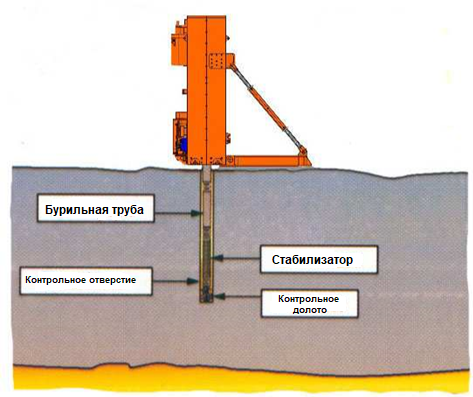
\includegraphics[width=0.8\textwidth]{assets/1121}
	\caption*{}
\end{figure}

{\bfseries Рис. 1- Бурение направляющей скважины станком «RHINO 2007 DC»}

Далее с бурильной колонны снимается пилотное долото, затем монтируется
расширительная головка. После скважину бурят до необходимого по проекту
диаметра (рисунок 2).

\begin{figure}[H]
	\centering
	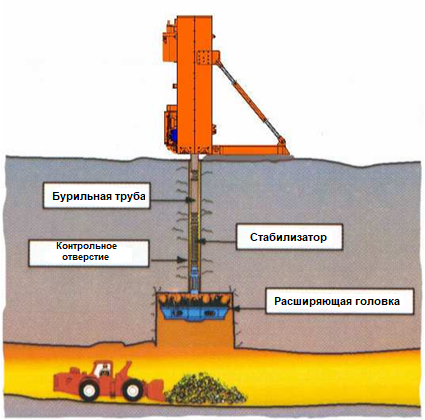
\includegraphics[width=0.8\textwidth]{assets/1122}
	\caption*{}
\end{figure}

{\bfseries Рис. 2 - Разбуривание направляющей скважины до проектного
диаметра «RHINO 2007 DC»}

Нынешний технологии легко позволяют производить бурение восстающих
стволов диаметром 3-4 метра. Однако, что касается бурения более крупных
диаметров, стоит отметить, что внедрение этой технологии идет довольно
медленно. Несмотря на это, использование расширительных головок и
передовых технологий в бурении позволяет достичь более высокой
производительности при бурении стволов диаметром 5-6 метров с
положительным экономическим эффектом, чем это было ранее {[}3{]}.

Результаты многолетних исследований обеспечивают научно-методические
основы для проектирования и расчета жестких и канатных армировок
вертикальных стволов в различных условиях. Были разработаны
безрасстрельные схемы армирования, методы крепления несущих элементов
армировки на анкерах, а также конструкции армировки с ограниченной
податливостью и возможностью радиального регулирования. В тот же период
эти решения были адаптированы для использования в стволах с монолитной
бетонной крепью. Однако теоретические и практические вопросы, связанные
с изучением совместной работы жесткой армировки и набрызгбетонной крепи,
остаются неизученными {[}5{]}.

Набрызгбетонная крепь характеризуется минимальной толщиной,
значительными отклонениями и неровностью контура, что создает сложности
при использовании стандартных жестких армировок ярусного типа и
негативно влияет на её прочностные и деформационные характеристики.
Несущие элементы армировки закрепляются в самой крепи и в окружающем
породном массиве, воздействие которого в существующих методиках расчета
армировки не учитывается. Кроме того, динамические воздействия от
движущихся подъемных сосудов не рассматриваются при определении
параметров набрызгбетонной крепи. Таким образом, возникает необходимость
в комплексном рассмотрении системы "безъярусная армировка -
набрызгбетонная крепь - породный массив" и последующем поиске и
обосновании эффективных решений для армирования глубоких вентиляционных
стволов.

Для крепления вертикальных выработок круглой формы при использовании
обычного метода проходки чаще всего используется монолитный бетон или в
некоторых случаях оставляется без крепления. В устьях и на участках,
проходимых специальными способами в слабых обводненных породах,
устанавливается металлическая тюбинговая крепь. Кроме того, в
зависимости от горно-геологических условий, вертикальные выработки по
всей длине могут быть закреплены железобетонной монолитной, тюбинговой
или набрызгбетонной крепями, а также временной штанговой (анкерной)
крепью с последующим усилением её постоянной бетонной или
набрызгбетонной крепью {[}5{]}.

При выборе конструкции и материала для крепи вертикальных стволов,
инженеры исходят из детального анализа геологических характеристик пород
и условий их расположения, таких как угол падения, трещиноватость и
другие факторы. Результаты исследований основных физико-механических
свойств окружающих пород позволяют определить прочность, угол
внутреннего трения, модуль упругости, пористость и другие характеристики
массива. Эти данные получают на основе изучения геологических
материалов, полученных в результате бурения контрольных разведочных
скважин. Кроме того, ценным и достаточно достоверным источником
информации при выборе конструкции крепи, особенно её толщины, является
обследование и анализ состояния крепи ранее построенных вертикальных
выработок в аналогичных горно-геологических условиях.

Выбор и расчет параметров податливой металлической рамной крепи горных
выработок вне зоны и в зоне влияния очистных работ по пологим,
наклонным, круто-наклонным и крутым платам определяют по Инструкции,
разработанной ВНИМИ в 1991 году.

По методике ВНИМИ, для прогноза устойчивости горизонтальных выработок
угольных шахт в качестве критерия устойчивости принимается величина
ожидаемых смещений на контуре сечения незакрепленной выработки за весь
срок ее службы, определяемых по формуле:

\begin{figure}[H]
	\centering
	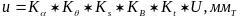
\includegraphics[width=0.8\textwidth]{assets/1123}
	\caption*{}
\end{figure} (1)

где u\textsubscript{т} - смещения (типовые), определяемые по графикам
(рисунок Д.1);

\begin{figure}[H]
	\centering
	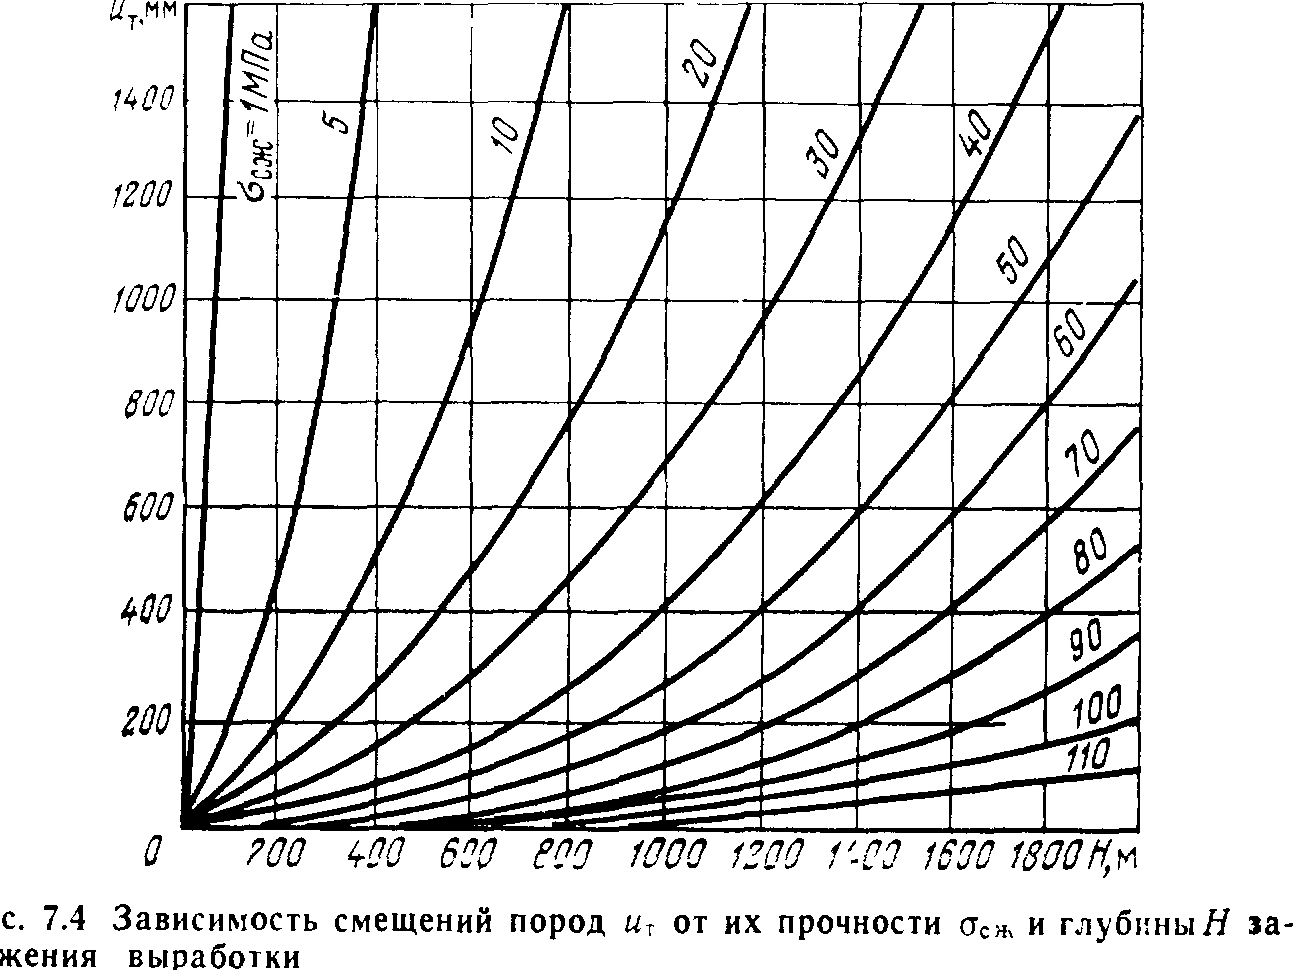
\includegraphics[width=0.8\textwidth]{assets/1124}
	\caption*{}
\end{figure}

{\bfseries Рис. 1 - Графики для определения типовых смещений пород}

К\textsubscript{α} -коэффициент влияния угла залегания пород и
на­правления проведения выработки относительно простирания по­род или
основных плоскостей трещиноватости, определяемый по таблице 1;

К\textsubscript{θ}-коэффициент, учитывающий направление сме­щений пород и
принимающий значение 1 при определении сме­щений со стороны кровли или
почвы (в вертикальном направ­лении). При определении боковых смещений
пород (в горизон­тальном направлении) К\textsubscript{θ} принимается по
таблице 1.

{\bfseries Таблица 1- Определение боковых смещений пород (в горизонтальном
направлении)}

\begin{longtable}[]{@{}
  >{\raggedright\arraybackslash}p{(\columnwidth - 20\tabcolsep) * \real{0.2257}}
  >{\raggedright\arraybackslash}p{(\columnwidth - 20\tabcolsep) * \real{0.0774}}
  >{\raggedright\arraybackslash}p{(\columnwidth - 20\tabcolsep) * \real{0.0720}}
  >{\raggedright\arraybackslash}p{(\columnwidth - 20\tabcolsep) * \real{0.0722}}
  >{\raggedright\arraybackslash}p{(\columnwidth - 20\tabcolsep) * \real{0.0722}}
  >{\raggedright\arraybackslash}p{(\columnwidth - 20\tabcolsep) * \real{0.0840}}
  >{\raggedright\arraybackslash}p{(\columnwidth - 20\tabcolsep) * \real{0.0796}}
  >{\raggedright\arraybackslash}p{(\columnwidth - 20\tabcolsep) * \real{0.0804}}
  >{\raggedright\arraybackslash}p{(\columnwidth - 20\tabcolsep) * \real{0.0764}}
  >{\raggedright\arraybackslash}p{(\columnwidth - 20\tabcolsep) * \real{0.0894}}
  >{\raggedright\arraybackslash}p{(\columnwidth - 20\tabcolsep) * \real{0.0706}}@{}}
\toprule\noalign{}
\endhead
\bottomrule\noalign{}
\endlastfoot
\multirow{3}{=}{Направление

проходки

выработки} &
\multicolumn{10}{>{\raggedright\arraybackslash}p{(\columnwidth - 20\tabcolsep) * \real{0.7743} + 18\tabcolsep}@{}}{%
Коэффициенты К\textsubscript{α} и К\textsubscript{θ} в зависимости от
угла падения пород α, град} \\
&
\multicolumn{2}{>{\raggedright\arraybackslash}p{(\columnwidth - 20\tabcolsep) * \real{0.1494} + 2\tabcolsep}}{%
до 20} &
\multicolumn{2}{>{\raggedright\arraybackslash}p{(\columnwidth - 20\tabcolsep) * \real{0.1445} + 2\tabcolsep}}{%
21-30} &
\multicolumn{2}{>{\raggedright\arraybackslash}p{(\columnwidth - 20\tabcolsep) * \real{0.1636} + 2\tabcolsep}}{%
31-40} &
\multicolumn{2}{>{\raggedright\arraybackslash}p{(\columnwidth - 20\tabcolsep) * \real{0.1568} + 2\tabcolsep}}{%
41-50} &
\multicolumn{2}{>{\raggedright\arraybackslash}p{(\columnwidth - 20\tabcolsep) * \real{0.1600} + 2\tabcolsep}@{}}{%
более 50} \\
& К\textsubscript{α} & К\textsubscript{θ} & К\textsubscript{α} &
К\textsubscript{θ} & К\textsubscript{α} & К\textsubscript{θ} &
К\textsubscript{α} & К\textsubscript{θ} & К\textsubscript{α} &
К\textsubscript{θ} \\
По простиранию & 1 & 0,35 & 0,95 & 0,55 & 0,8 & 0,8 & 0,65 & 1,2 & 0,6 &
1,5 \\
вкрест простирания & 0,7 & 0,55 & 0,6 & 0,8 & 0,45 & 0,95 & 0,25 & 0,95
& 0,2 & 0,8 \\
под углом к простиранию & 0,85 & 0,45 & 0,8 & 0,65 & 0,65 & 0,9 & 0,45 &
1,05 & 0,35 & 1,1 \\
\end{longtable}

К\textsubscript{S} - ко­эффициент влияния пролета выработки для кровли и
почвы принимается равным К\textsubscript{S} \emph{=} 0,2 (b-1), для
боков выработки К\textsubscript{S} \emph{=} 0,2 (h-1) (b - пролет
выработки, h- высота выработки);

К\textsubscript{В} - коэффициент влияния других вы­работок, равный для
одиночных выработок 1; для сопряжений с односторонним примыканием
выработки-1,4; для сложных сопряжений с примыканием выработок в виде
двустороннего заезда или пересекающихся выработок-1,6. Для параллель­ных
выработок этот коэффициент равен:

\begin{figure}[H]
	\centering
	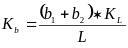
\includegraphics[width=0.8\textwidth]{assets/1125}
	\caption*{}
\end{figure} (2)

где L- расстояние между выработками, м;

b\textsubscript{1} и b\textsubscript{2} пролеты взаимовлияющих
выработок, м

К\textsubscript{L} коэффициент, принимаемый по табл. 2.2;

{\bfseries Таблица 2 - Определение коэффициента направления проходки
выработок К\textsubscript{L}}

\begin{longtable}[]{@{}
  >{\raggedright\arraybackslash}p{(\columnwidth - 20\tabcolsep) * \real{0.2257}}
  >{\raggedright\arraybackslash}p{(\columnwidth - 20\tabcolsep) * \real{0.0774}}
  >{\raggedright\arraybackslash}p{(\columnwidth - 20\tabcolsep) * \real{0.0720}}
  >{\raggedright\arraybackslash}p{(\columnwidth - 20\tabcolsep) * \real{0.0722}}
  >{\raggedright\arraybackslash}p{(\columnwidth - 20\tabcolsep) * \real{0.0722}}
  >{\raggedright\arraybackslash}p{(\columnwidth - 20\tabcolsep) * \real{0.0840}}
  >{\raggedright\arraybackslash}p{(\columnwidth - 20\tabcolsep) * \real{0.0796}}
  >{\raggedright\arraybackslash}p{(\columnwidth - 20\tabcolsep) * \real{0.0804}}
  >{\raggedright\arraybackslash}p{(\columnwidth - 20\tabcolsep) * \real{0.0764}}
  >{\raggedright\arraybackslash}p{(\columnwidth - 20\tabcolsep) * \real{0.0894}}
  >{\raggedright\arraybackslash}p{(\columnwidth - 20\tabcolsep) * \real{0.0706}}@{}}
\toprule\noalign{}
\endhead
\bottomrule\noalign{}
\endlastfoot
\multirow{3}{=}{Направление

проходки

выработки} &
\multicolumn{10}{>{\raggedright\arraybackslash}p{(\columnwidth - 20\tabcolsep) * \real{0.7743} + 18\tabcolsep}@{}}{%
Коэффициенты К\textsubscript{α} и К\textsubscript{θ} в зависимости от
угла падения пород α, град} \\
&
\multicolumn{2}{>{\raggedright\arraybackslash}p{(\columnwidth - 20\tabcolsep) * \real{0.1494} + 2\tabcolsep}}{%
до 20} &
\multicolumn{2}{>{\raggedright\arraybackslash}p{(\columnwidth - 20\tabcolsep) * \real{0.1445} + 2\tabcolsep}}{%
21-30} &
\multicolumn{2}{>{\raggedright\arraybackslash}p{(\columnwidth - 20\tabcolsep) * \real{0.1636} + 2\tabcolsep}}{%
31-40} &
\multicolumn{2}{>{\raggedright\arraybackslash}p{(\columnwidth - 20\tabcolsep) * \real{0.1568} + 2\tabcolsep}}{%
41-50} &
\multicolumn{2}{>{\raggedright\arraybackslash}p{(\columnwidth - 20\tabcolsep) * \real{0.1600} + 2\tabcolsep}@{}}{%
более 50} \\
& К\textsubscript{α} & К\textsubscript{θ} & К\textsubscript{α} &
К\textsubscript{θ} & К\textsubscript{α} & К\textsubscript{θ} &
К\textsubscript{α} & К\textsubscript{θ} & К\textsubscript{α} &
К\textsubscript{θ} \\
По простиранию & 1 & 0,35 & 0,95 & 0,55 & 0,8 & 0,8 & 0,65 & 1,2 & 0,6 &
1,5 \\
вкрест простирания & 0,7 & 0,55 & 0,6 & 0,8 & 0,45 & 0,95 & 0,25 & 0,95
& 0,2 & 0,8 \\
под углом к простиранию & 0,85 & 0,45 & 0,8 & 0,65 & 0,65 & 0,9 & 0,45 &
1,05 & 0,35 & 1,1 \\
\end{longtable}

К\textsubscript{t} - коэффициент влияния времени, принимаемый равным 1
для выработок, срок службы которых более 15 лет, и по графикам 2, 3.

\begin{figure}[H]
	\centering
	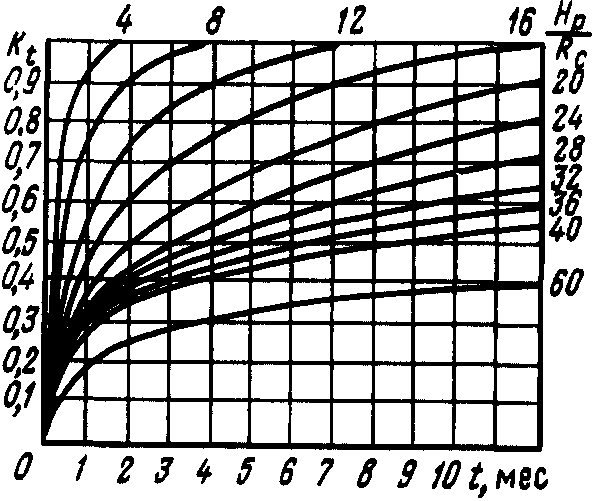
\includegraphics[width=0.8\textwidth]{assets/1126}
	\caption*{}
\end{figure}

{\bfseries Рис. 2 - Графики для определения коэффициента К\textsubscript{t}
при сроке службы выработки более года}

\begin{figure}[H]
	\centering
	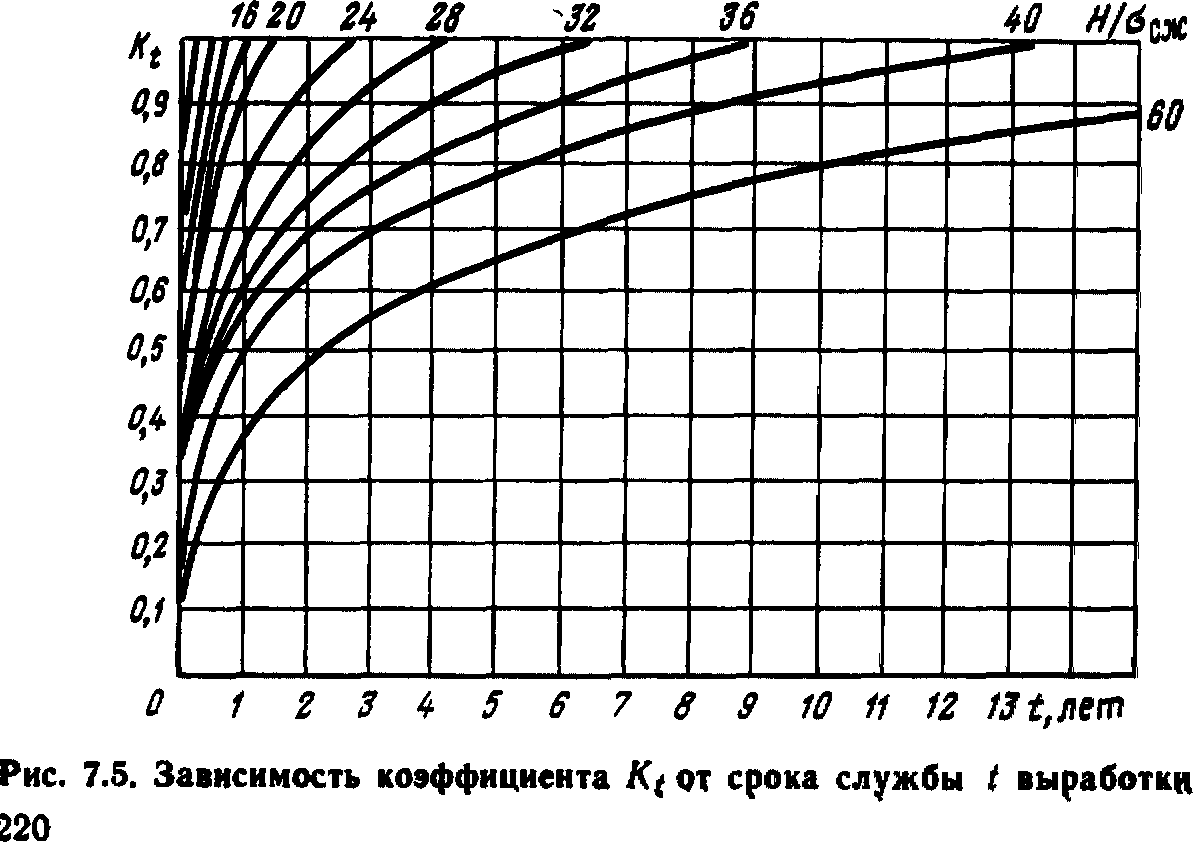
\includegraphics[width=0.8\textwidth]{assets/1127}
	\caption*{}
\end{figure}

{\bfseries Рис. 3 - Графики для определения коэффициента К\textsubscript{t}
при сроке службы выработки менее года}

Согласно Инструкции ВНИМИ расчетная нагрузка \emph{P} на крепь выработок
как вне зоны влияния очистных работ, так и в зоне влияния очистных работ
определяется исходя из расчетной величины смещений пород кровли, почвы и
боков выработки. Плотность \emph{n} установки рам металлической
податливой крепи на 1 м длины выработки определяют из выражения:

\begin{figure}[H]
	\centering
	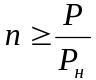
\includegraphics[width=0.8\textwidth]{assets/1128}
	\caption*{}
\end{figure} (3)

где \emph{P} -- расчетная нагрузка, к\emph{Н}:

\emph{P}\textsubscript{н} -- несущая способность (сопротивление) рамы,
к\emph{Н}.

Инструкцией предлагается паспортную плотность установки крепи принимать
по ближайшему значению числа рам \emph{n} на 1 м длины выработки в ряду:
0,8; 1; 1,25; 1,33; 1,43; 1,67; 2; 2,25; 2,5; 2,67; 3; 4. Предельной
плотностью податливой металлической рамной крепи рекомендуется считать 3
рамы/м. Методика определения смещений пород в горных выработках,
охраняемых различными способами и испытывающих влияние очистных работ,
изложена в Инструкции.

Нормативные нагрузки на незамкнутую крепь определяют по графикам рис 4 в
зависимости от смещений пород U и ширины выработки в проходке. Если
свойства пород в боках выработки различны, то ожидаемые смещения U и
определяемые по смещениям нормативные нагрузки боковые нагрузки также
будут отличаться друг от друга. В этом случае для дальнейших расчетов
принимают усредненное значение нормативной нагрузки со стороны боков и
нормативную нагрузку со стороны почвы.

Нормативные нагрузки на замкнутую крепь также определяются по графикам
рис. 4 отдельно для кровли, почвы и боков. Усредненная вертикальная
нагрузка определяется по значениям нормативных нагрузок со стороны
кровли и почвы, усредненная горизонтальная нагрузка - по значениям
нормативных нагрузок со стороны боков.

Расчетная нагрузка на 1 м выработки со стороны боков определяется по
формуле:

\begin{figure}[H]
	\centering
	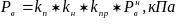
\includegraphics[width=0.8\textwidth]{assets/1129}
	\caption*{}
\end{figure} (4)

где k\textsubscript{п}- коэффициент перегрузки, учитывающий изменчивость
нагрузки (таблица 3);

k\textsubscript{н}- коэффициент, принимаемый для главных вскрывающих
выработок равным 1,1; для остальных-1;

k\textsubscript{пр}- коэффициент условий проведения выработок,
принимаемый равным 1 при проведении выработок буровзрывным способом. При
комбай­новом способе проведения выработок принимается по таблице 4;

Р\textsuperscript{н}\textsubscript{в}- нормативная вертикальная
нагрузка.

Если свойства пород в боках выработки различны, то ожидаемые смещения U
и определяемые по смещениям нормативные нагрузки боковые нагрузки также
будут отличаться друг от друга.

{\bfseries Таблица 3 - Значения коэффициента k\textsubscript{п}}

\begin{longtable}[]{@{}
  >{\raggedright\arraybackslash}p{(\columnwidth - 4\tabcolsep) * \real{0.2155}}
  >{\raggedright\arraybackslash}p{(\columnwidth - 4\tabcolsep) * \real{0.3911}}
  >{\raggedright\arraybackslash}p{(\columnwidth - 4\tabcolsep) * \real{0.3934}}@{}}
\toprule\noalign{}
\endhead
\bottomrule\noalign{}
\endlastfoot
\multirow{2}{=}{U, мм} &
\multicolumn{2}{>{\raggedright\arraybackslash}p{(\columnwidth - 4\tabcolsep) * \real{0.7845} + 2\tabcolsep}@{}}{%
значения {\bfseries k\textsubscript{п}} для выработок} \\
& вскрывающих & Подготавливающих \\
до 50 & 1,25 & 1,1 \\
51-200 & 1,1 & 1,05 \\
201-500 & 1,05 & 1 \\
более 500 & 1 & 1 \\
\end{longtable}

{\bfseries Таблица 4 - Значения коэффициента k\textsubscript{пр}}

\begin{longtable}[]{@{}
  >{\raggedright\arraybackslash}p{(\columnwidth - 8\tabcolsep) * \real{0.1463}}
  >{\raggedright\arraybackslash}p{(\columnwidth - 8\tabcolsep) * \real{0.2278}}
  >{\raggedright\arraybackslash}p{(\columnwidth - 8\tabcolsep) * \real{0.2278}}
  >{\raggedright\arraybackslash}p{(\columnwidth - 8\tabcolsep) * \real{0.2278}}
  >{\raggedright\arraybackslash}p{(\columnwidth - 8\tabcolsep) * \real{0.1702}}@{}}
\toprule\noalign{}
\endhead
\bottomrule\noalign{}
\endlastfoot
{\bfseries Н\textsubscript{р}/R\textsubscript{c}} & до 16 & более 16 до 20
& более 20 до 25 & более 25 \\
{\bfseries k\textsubscript{пр}} & 0,6 & 0,8 & 1,0 & 1,1 \\
\end{longtable}

Расчетная нагрузка на 1 м выработки со стороны боков определяется по
формуле:

\begin{figure}[H]
	\centering
	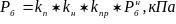
\includegraphics[width=0.8\textwidth]{assets/1130}
	\caption*{}
\end{figure} (5)

где Р\textsuperscript{н}\textsubscript{б}- нормативная горизонтальная
нагрузка, кПа.

{\bfseries В=6 м}

{\bfseries В=5 м}

{\bfseries В=4 м}

{\bfseries Рис. 4 -- Графики определения нормативной нагрузки на крепь}

{\bfseries Результаты и обсуждение.} Технический результат заключается в
повышении эффективности крепления шахтного ствола за счет конструкции,
включающей в себя кольцевую крепь, размещённую в специальной нише
ствола, закрепленную анкерами. Для предотвращения вывалов породы,
устанавливается сетка, в местах геологических нарушений дополнительно
применяется набрызгбетонная крепь {[}6{]}.

В пройденном участке устья ствола монтируется подвесной проходческий
полок, для чего предусматривается установить временное перекрытие для
монтажа проходческого полка.

Крепление участка устья ствола производится монолитным железобетоном с
помощью инвентарной опалубки с рабочей высотой 0,9÷1,0 м

Постоянная крепь пройденного ранее участка устья ствола возводится после
сооружения опорного венца снизу-вверх. Бетон подается за опалубку по
временным ставам бетонопроводов, подвешенными на лебедках забойного
бетонопровода. Для равномерной укладки бетона по всему периметру ствола
на концы бетонопроводов навешиваются гибкие гофрированные рукава
необходимого диаметра.

По мере возведения постоянной крепи временную крепь демонтируют и
извлекают на поверхность. \emph{{\bfseries Бетонированию}} подлежат боковые
породы за контуром постоянной железобетонной крепи на устье ствола
{[}7{]}.

Кольцевая крепь представляет собой разновидность рамной крепи с
замкнутым контуром, состоящей из отдельных колец, установленных вдоль
выработки вразбежку и связанных между собой при помощи стяжек (подвесок)
или распорок, и применяемой в горизонтальных, наклонных и вертикальных
выработках при наличии всестороннего смещения массива горных пород.
Кольцевую крепь классифицируют по площади сечения выработок (от 6,5 до
20,1 м), по конструктивному исполнению (жесткие, шарнирные и податливые)
и применяемому прокату и марке стали {[}8{]}.

Устье ствола 1 бетонируется. В месте монтажа кольцевой крепи выбирается
ниша 2 диаметром не менее R+300 мм, где R -- диаметр ствола. В нишу
устанавливается кольцевая крепь 3. Кольцевая крепь между собой соединена
при помощи стальных расстрелов и проводников 4 {[}9{]}.

Далее устанавливается пластиковая либо металлическая сетка 5 (для
предотвращение осыпаний), после чего производится крепление анкерами 6,
как кольцевой крепи, так и межрамного пространства (Рисунок 3).

\begin{figure}[H]
	\centering
	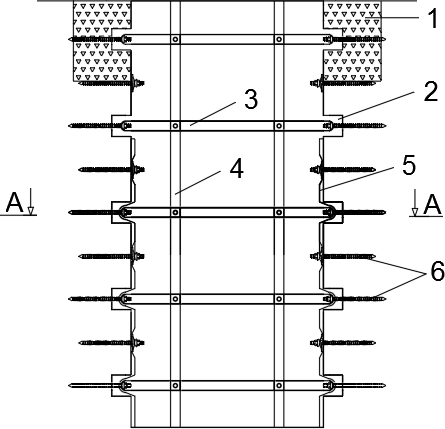
\includegraphics[width=0.8\textwidth]{assets/1131}
	\caption*{}
\end{figure}
\begin{figure}[H]
	\centering
	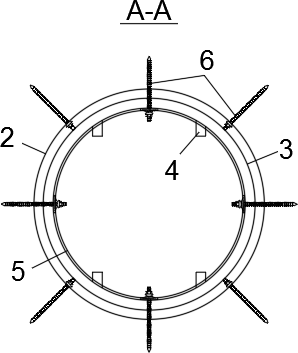
\includegraphics[width=0.8\textwidth]{assets/1132}
	\caption*{}
\end{figure}

{\bfseries Рис. 3 - Разработанная технология крепления ствола}

Процесс установки анкеров включает несколько этапов, таких как бурение
шпуров, подготовка раствора, наполнение шпуров раствором и закладка
арматурных стержней. Расположение шпуров для установки штанг должно
соответствовать указаниям в паспорте крепления.

При установке анкеров через металлическую сетку, которую необходимо
закрепить в углублениях породного обнажения, допускается отклонение
расстояния между анкерами до 30 \%.

Для обеспечения надежного сцепления цементно-песчаного раствора с
породой в стенках шпуров, необходимо тщательно продуть шпуры сжатым
воздухом или промыть их водой с целью полного удаления буровой мелочи и
пыли.

Цементно-песчаный раствор для анкеров готовят с использованием
растворомешалки или вручную, после чего подают в шпур при помощи
пневмонагнетателя сжатым воздухом через резиновый шланг и металлическую
трубу диаметром 18-25 мм. Длина трубы должна быть не меньше глубины
шпура. Трубку вводят в шпур до его забоя, и в процессе заполнения шпура
раствором её постепенно вытаскивают из шпура {[}10{]}.

Процедура заполнения шпура раствором должна обеспечивать полное
закрепление анкера по всей его длине.

{\bfseries Выводы.} Проведенный анализ технических и технологических
решений крепи и армировки стволов позволил сформулировать объект и
предмет, область применения научных и практических результатов, а также
сделать следующие основные выводы:

1. В вентиляционных стволах угольных шахт и рудников, отнесенных к I и
II категории устойчивости, целесообразно применять ресурсосберегающую
набрызгбетонную крепь. Она достаточно широко использовалась в нашей
стране в 70-80 годы прошлого века. Однако в последние 20 лет для
крепления стволов глубиной более 700 м в устойчивых породах применяется
только монолитная бетонная крепь. Одной из причин такого положения
является отсутствие эффективных технических и технологических решений
жесткой армировки, адаптированных для применения в стволах, закрепленных
набрызгбетоном.

2. Канатная армировка может успешно применяться в стволах с любым типом
крепи, но с увеличением их глубины зачастую возникает необходимость
увеличения диаметра ствола, также существенно возрастает масса
направляющих канатов и натяжных устройств, что делает неэффективным ее
применение.

3. Определена область применения кольцевой крепи с упрочняющей анкерной
крепью в более склонных к ползучести аргиллитах. Для ее увеличения
целесообразно применение цементных анкеров с ограниченной податливостью.

{\bfseries Литература}

1. Геотехнология строительная: методические указания. -Донецк: Донецкий
национальный технический университет, 2017.

2.Технологический регламент (инструкция) по выбору типов и параметров
крепей и технологии их возведения на Артемьевском месторождении --
Караганда: ТОО «Mining Research Group», 2015.-108 с.

3.Бабец, Д.В. Применение метода группового учета аргументов к задаче
оценки устойчивости горной выработки // Горный
информационно-аналитический бюллетень. -2001. - №11. -С. 67-69.

4.Басакевич, С.В. Обоснование параметров безрасстрельной армировки
вертикальных стволов на основе вероятностной оценки временных нагрузок:
дис. ... канд. техн. наук: 25.00.22 / Басакевич Сергей Владимирович. -
Новочеркасск, 2009. - 145 с.

5. Dahlin, T. The development of DC resistivity imaging techniques //
Computers \& Geosciences. -- 2001. - Vol. 27. --P. 1019--1029. DOI
10.1016/S0098-3004(00)00160-6

6. Бобачев, А.А. Электроразведка: пособие по электроразведочной практике
для студентов геофизических специальностей. Том II Малоглубинная
электроразведка. Изд. 2-е, перераб. и доп. / Бобачев А.А. и др. - М.:
МГУ-2013. -123 с. ISBN:~978-5-904807-21-4

7. Груздев А.А., Науменко Д.А.,. Богданов П.С, Бобачев А.А., Шевнин В.А.
Бесконтактное измерение электрического поля с помощью OHMMAPPER в
условиях крайнего севера.// Электронный журнал "Георазрез", -2013. - №
01 (13). -С.1--23.

8. Loke M.H. Tutorial: 2-D and 3-D electrical imaging surveys.- URL :
www.geotomosoft.com (Revision date : 27th August 2021)

9. Адушкин В.В.,Спивак А.А., Кожухов С.А., Кукушкин Ю.В. Резонансные
особенности эсхаляции природного радона// Доклады РАН. -- 2005. - Т.400
(3). - С.369-371.

{\bfseries References}

1. Geotekhnologiya stroitel\textquotesingle naya: metodicheskie
ukazaniya. -Donetsk: Donetskii natsional\textquotesingle nyi
tekhnicheskii universitet, 2017. {[}in Russian{]}

2.Tekhnologicheskii reglament (instruktsiya) po vyboru tipov i
parametrov krepei i tekhnologii ikh vozvedeniya na
Artem\textquotesingle evskom mestorozhdenii -- Karaganda: TOO «Mining
Research Group», 2015.-108 s. {[}in Russian{]}

3.Babets, D.V. Primenenie metoda gruppovogo ucheta argumentov k zadache
otsenki ustoichivosti gornoi vyrabotki // Gornyi
informatsionno-analiticheskii byulleten\textquotesingle. -2001. - №11.
-S. 67-69. {[}in Russian{]}

4.Basakevich, S.V. Obosnovanie parametrov
bezrasstrel\textquotesingle noi armirovki vertikal\textquotesingle nykh
stvolov na osnove veroyatnostnoi otsenki vremennykh nagruzok: dis. ...
kand. tekhn. nauk: 25.00.22 / Basakevich Sergei Vladimirovich. -
Novocherkassk, 2009. - 145 s. {[}in Russian{]}

5. Dahlin, T. The development of DC resistivity imaging techniques //
Computers \& Geosciences. -- 2001. - Vol. 27. --P. 1019--1029. DOI
10.1016/S0098-3004(00)00160-6 {[}in Russian{]}c

6. Bobachev, A.A. Elektrorazvedka: posobie po elektrorazvedochnoi
praktike dlya studentov geofizicheskikh spetsial\textquotesingle nostei.
Tom II Maloglubinnaya elektrorazvedka. Izd. 2-e, pererab. i dop. /
Bobachev A.A. i dr. - M.: MGU-2013. -123 s. ISBN: 978-5-904807-21-4
{[}in Russian{]}

7. Gruzdev A.A., Naumenko D.A.,. Bogdanov P.S, Bobachev A.A., Shevnin
V.A. Beskontaktnoe izmerenie elektricheskogo polya s
pomoshch\textquotesingle yu OHMMAPPER v usloviyakh krainego severa.//
Elektronnyi zhurnal "Georazrez", -2013. - № 01 (13). -S.1--23. {[}in
Russian{]}

8. Loke M.H. Tutorial: 2-D and 3-D electrical imaging surveys.- URL :
www.geotomosoft.com (Revision date : 27th August 2021)

9. Adushkin V.V.,Spivak A.A., Kozhukhov S.A., Kukushkin Yu.V.
Rezonansnye osobennosti eskhalyatsii prirodnogo radona// Doklady RAN. --
2005. - T.400 (3). - S.369-371. {[}in Russian{]}

\emph{{\bfseries Сведения об авторах}}

Мусин Р. А. -PhD доктор, и.о. доцента, Карагандинский технический
университет имени Абылкаса Сагинова, Караганда, Казахстан, e-mail:
R.A.Mussin@mail.ru;

Асанова Ж.М. - PhD доктор, и.о. доцента, Карагандинский технический
университет имени Абылкаса Сагинова, Караганда, Казахстан, e-mail:
zhanar-a@bk.ru;

Байкенжин М. А. - PhD доктор, доцент, Карагандинский технический
университет имени Абылкаса Сагинова, Караганда, Казахстан, e-mail:
nailzamaliev@mail.ru

Альжанов Р.Х. - докторант группы ГДД-21, Карагандинский технический
университет имени Абылкаса Сагинова, Караганда, Казахстан, e-mail:
rushair@mail.ru.

\emph{{\bfseries Information about the authors}}

Musin R. A. - PhD, acting Associate Professor of the Abylkas Saginov
Karaganda Technical University, Karaganda, Kazakhstan, e-mail:
R.A.Mussin@mail.ru;

Asanova Zh. M.- PhD, acting Associate Professor of the Abylkas Saginov
Karaganda Technical University, Karaganda, Kazakhstan, e-mail:
zhanar-a@bk.ru;

Baikenzhin M. A.- candidate of technical sciences, associate professor
of the Abylkas Saginov Karaganda Technical University, Karaganda,
Kazakhstan, e-mail: mbmqm@mail.ru;

Alzhanov R.H. - doctoral student group GDD-21 Abylkas Saginov Karaganda
Technical University, Karaganda, Kazakhstan, e-mail: rushair@mail.ru.

{\bfseries \hfill\break
}

ҒТАMР 52.35.29

{\bfseries КӨМІР ҚАБАТЫНДАҒЫ ЖЕРАСТЫ ГАЗСЫЗДАНДЫРУ ҰҢҒЫМАЛАРЫНАН}

{\bfseries ГАЗ ШЫҒУЫН АРТТЫРУ}

{\bfseries М.С.Усенбеков\textsuperscript{🖂}, Е.М. Мейрам, М.Н. Жумабеков,
М. Рабатұлы, Т.К. Исабек}

Әбілқас Сағынов атындағы Қарағанды техникалық университеті, Қарағанды,
Қазақстан,

{\bfseries \textsuperscript{🖂}} Корреспондент-автор: meirambek46@mail.ru

Бұл жұмыста қабаттың газ шығуын арттыру үшін көмір қабатын гидравликалық
айыру әдісін қолдану нәтижелері келтірілген. Бұл ретте диаметрі 93 мм
және ұзындығы 40-80 метр ұңғымалар арқылы 300 атм аспайтын қысыммен
пакерлер арқылы шахта суы айдалды. Гидравликалық айыру әдісіне дейін
және одан кейін ұңғымалардың аузындағы өлшеулер көмір қабатынан газ
шығуының орта есеппен 1,8 есе артқанын көрсетті.

{\bfseries Түйін сөздер:} көмір қабаты, газ шығуы, гидравликалық айыру
әдісі, шахта, ұңғыма, жарықшалар, метан.

{\bfseries INCREASING THE GAS OUTPUT OF UNDERGROUND DEGASSING WELLS IN THE
COAL SEAM}

{\bfseries M.S.\textsuperscript{.}Usenbekov\textsuperscript{🖂}, E.M.
Meiram, M.N.Zhumabekov, M.Rabatuly, T.K.Isabek}

Abylkas Saginov Karaganda Technical University, Karaganda, Kazakhstan,

e-mail: meirambek46@mail.ru

This paper presents the results of the application of hydraulic
fracturing of a coal seam to increase its gas recovery. At the same
time, mine water was pumped through wells with a diameter of 93 mm and a
length of 40-80 meters at a pressure of no more than 300 atm through
packers. Measurements at the wellhead before and after hydraulic
fracturing showed an increase in coal seam gas recovery by an average of
1.8 times.

{\bfseries Keywords:} coal seam, gas release, hydraulic fracturing, mine,
well, fractures, methane

{\bfseries ПОВЫШЕНИЯ ГАЗООТДАЧИ ПОДЗЕМНЫХ ДЕГАЗАЦИОННЫХ СКВАЖИН В УГОЛЬНОМ
ПЛАСТЕ}

{\bfseries М.С.Усенбеков\textsuperscript{🖂}, Е.М.Мейрам, М.Н.Жумабеков,
М.Рабатұлы, Т.К.Исабек}

Карагандинский технический университет им. Абылкаса Сагинова, Караганда,
Казахстан,

е-mail: meirambek46@mail.ru

В данной работе приведены результаты применения гидроразрыва угольного
пласта для повышения его газоотдачи. При этом через скважины диаметром
93 мм и длиной 40-80 метров под давлением не более 300 атм через пакеры
закачивалась шахтная вода. Замеры на устье скважин до и после
гидроразрыва показали увеличение газоотдачи угольного пласта в среднем в
1,8 раза.

{\bfseries Ключевые слова:} угольный пласт, газовыделение, гидравлический
разрыв, шахта, скважина, трещины, метан.

{\bfseries Кіріспе.} Көмір қабаттарын игеру тереңдігінің артуымен
газ-динамикалық құбылыстардың қаупі жоғарылап, кенжарға газ шығарудың
артуы байқалады, бұл көмір өндіру қарқынын тежейді және тау-кен
жұмыстарының қауіпсіздігін төмендетеді. Көмір метанның белгілі бір
мөлшерін тиісті қысым мен температурада байланыстырылған күйде ұстай
алады. Көмірден метанды алу сорбциялық тепе-теңдік бұзылған және газ
ұңғымаларға қарай жылжитын көміртегі массивінің өткізгіштігі жоғарылаған
жағдайда ғана мүмкін болады.

Әлемдік тәжірибеде газсыздандыруды қарқындату әдістерін талдау көмір
қабаттарының газ шығару қабылетін өсіру үшін қабатты гидравликалық айыру
әдісін (ҚГАӘ) жиі қолданылатынын көрсетеді {[}1,2,3,4{]}. ҚГАӘ
процесінде пайда болған жарықшалар ұзындығы бірнеше ондаған метрге жетуі
мүмкін, бір-бірімен және басқа жарықшалармен байланысып, массивтің
өткізгіштігін едәуір арттырады. Бұл әдіс бүгінгі күнге дейін
ұңғымалардан газ шығуын арттырудың ең тиімді әдісі болып табылады
{[}5,6,7,8{]}.

Шахта жағдайында гидравликалық айыру әдісі көмір қабатын газсыздандыру
мерзімдерін азайту мақсатында және көмір қабаттарының алдын-ала
газсыздандыру дәрежесін арттыру үшін қолданылады. Оның мәні көмір
қабатында тау жыныстарының массивін ішінара түсіруге, онда тау
жыныстарын газсыздандыру үшін сүзгі арналарын құруға арналған жарықтар
жүйесін қалыптастырудан тұрады.

{\bfseries Материалдар мен әдістер.} Қазіргі уақытта көмір қабатын игеру
алдында конвейерлік және желдету штректері маңында бұрғыланған ұңғымалар
арқылы алдын ала газсыздандыру жүргізіледі, содан кейін оларды 6 ай бойы
вакуумдық сорғы станциясына қосады. Бұл әдістің кемшілігі ұңғымалардың
қабырғалары арқылы ұңғыма маңындағы көмір қабатының өте кішкентай
аймағынан газ шығарылады. Сондықтан көмір қабаттарынан газды бұл әдіспен
алу тиімділігі осы жағдайларда қауіпсіз жұмысты қамтамасыз ету үшін
жеткіліксіз {[}9{]}. Көмір қабатының газдылығын төмендетудің негізгі
әдісі - газсыздандыру ұңғымаларын дайындық қазбаларынан қазба бағанының
денесіне бұрғылау. Тәжірибе көрсеткендей, белсенді газ шығару кезеңі
және жалпы газсыздандыру ұңғымасының тиімділігі өте аз, бұл қабаттың
физика-механикалық қасиеттеріне байланысты. Көмір қабатын ұңғыма арқылы
газ шығару процесін гидроайыру жарықшақтарын қалыптастыру арқылы оған
қосымша әсер ету беттерін жасау арқылы күшейтуге болады. Көмір қабатының
газ шығынын арттыру арқылы алдын ала газсыздандырудың тиімділігін
арттыру үшін жақында көмір массивінің гидроайыруы қолданылады. Көмір
қабатын ұңғыма арқылы газ шығару процесін гидроайыру жарықтарын
қалыптастыру арқылы оған қосымша әсер ету беттерін жасау арқылы
күшейтуге болады.

Гидравликалық айыру әдісін орындау үшін арнайы бұрғыланған жерасты
ұңғымаларын қолданады. Станок 1 (1-сурет) бұрғыланған көмір массивіндегі
3 ұңғымаларды 2 контурлау қазбаларынан тазарту кенжарына 4 параллель
бұрғылайды, мысалы, конвейер штрегінен 5 желдету штрегіне 6 дейін. Содан
кейін конвейерлік штрек 5 жағынан ұңғымада 2 бұрғылау қондырғысы бар
жабдықты 7, тығыздағыш 9 құрылғысы бар саңылаутүзгішті 8 монтаждау
жүргізіледі. Икемді құбыр 10 арқылы тығыздағыш құрылғы 9 желдеткіш
штректе 6 орналасқан сорғы станциясына 11 қосылады. Әрі қарай, конвейер
штрегінің 5 жағында бастаушы саңылаулар 12 кесіліп, тығыздағыш құрылғы 9
бен саңылау түзгіштің 8 ұзындығының қосындысына тең әрі L-қадаммен
саңылаулар түзеді. Бұл әрбір келесі бастау саңылауын 12 кесу кезінде
әрбір алдыңғы саңылаутүзушіні тығыздауға және айыруға мүмкіндік береді,
бұл саңылаутүзушіні кесу және гидроайыру операцияларын біріктіруге
мүмкіндік береді. Сорғы станциясының 11 кесілген инициативті
саңылауларын 12 икемді құбыр 10 арқылы қысыммен тығыздағыш құрылғыға 9
айыру үшін жұмыс сұйықтығы беріледі - инициативті саңылау 12 орналасқан
ұңғыма аймағы тығыздалады. Тығыздағыш құрылғы 9 орнатылған қысым
деңгейінен асып кеткен кезде, жұмыс сұйықтығы инициативті саңылауға 12
жіберіледі және гидроайыру жарықшақтары пайда болады.

\begin{figure}[H]
	\centering
	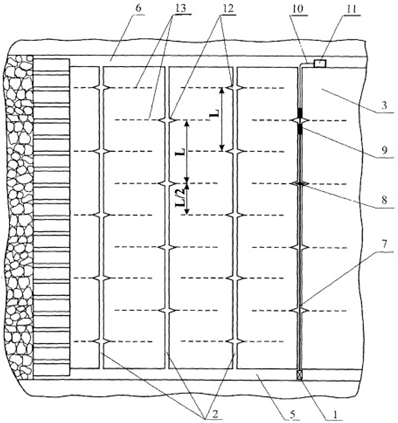
\includegraphics[width=0.8\textwidth]{assets/1133}
	\caption*{}
\end{figure}

{\bfseries 1-сурет - Гидравликалық айыру әдісімен газдың шығыуын ұлғайту
схемасы:}

\emph{1-станок; 2-ұңғыма; 3-көмір массиві; 4-тазарту кенжары; 5-конвейер
штрегі; 6- желдету штрегі; 7-бұрғылау қондырғы; 8-саңылау түзгіш;
9-тығыздағыш құрылғы; 10-құбыр; 11-сорғы станциясы; 12-инициативті
саңылау; 13-гидроайыру жарықшақтары; L-саңылау түзгіштер аралығы}

Көмір массивін 3 гидроайыру бойынша жұмыстар аяқталғаннан кейін бірінші
ұңғыманың 2 бүкіл ұзындығы бойынша оған іргелес келесі ұңғымадағы 2
ұқсас жұмыстарға ауысады, бұл ретте инициативті саңылауларды 12 кесу сол
әдіспен және L кесу қадамымен жүргізіледі. Алайда, кейінгі ұңғымадағы 2
инициативті саңылауларды 12 кесу алдыңғы ұңғыманың 2 инициативті
саңылауларына 12 қатысты кесу қадамын инициативті саңылаулар 12
арасындағы қашықтықтың жартысына тең шамаға ауыстыра отырып жүзеге
асырылады. Осылайша, іргелес ұңғымалардың көмір массивінің гидроайыру
жарықшақтары 13 арасындағы қашықтық екі есе азаяды және L/2-ге (1-сурет)
тең болады, сондықтан көмір массивінің әсер ету аймағы екі есе көп
болады, бұл көмір қабатын кейінгі газсыздандыру тиімділігін арттырады.

Кейінгі ұңғымалар 2 бірдей ретпен өңделеді. Бұл ретте бұрғыланған
ұңғымаларда оның бүйір бетіндегі инициативті саңылаулар кесіледі,
ұңғыманың үзілу аралығы арнайы пакермен тығыздалады, содан кейін көмірде
жарықшақтар пайда болуы үшін қысыммен суды үзіліс аралығына айдайды. Бұл
жағдайда инициативті саңылауды кесу кезінде пайда болған көмір
бөлшектері ұңғыманың үзілу аралығында ұсталады, айдалатын сумен
араластырылады және алынған суспензия жарықшаққа айдалады. Техникалық
нәтиже - газды көмір қабаттарын газсыздандыру тиімділігін арттыру болып
табылады.

Гидравликалық айыру әдісі диаметрі 93 мм, ұзындығы 40-80 метр
ұңғымаларда іске асырылды. Гидравликалық айыру ұңғымалары мен
газсыздандыру ұңғымалары судың айыру процесі тоқтағаннан кейін
газсыздандыру желісіне қосылды. ҚГАӘ-ның тиімділігі метанның шығуының
өсуіне дейін және одан кейін өлшенген дебиттерін салыстыру арқылы
анықталды. Сонымен қатар, «Казахстанская» шахтасында қабат ұңғымаларын
газсыздандыру желісіне қосу 10 ұңғымадан блокпен жүргізілді, онда ҚГАӘ
қолданумен немесе қолданусыз аудандарда метан дебиттеріне салыстыру
жүргізілді.

Қабатты гидравликалық айыру сорғының көмегімен шамамен 16 МПа қысыммен
айдалатын жұмыс сұйықтығымен жүзеге асырылады. Жұмыс сұйықтығы ретінде
шахта су құбырының суы қолданды {[}10{]}.

Қабатты гидравликалық айыру сұйықтықтың берілген көлемін қабатқа
айдағаннан кейін немесе оның штрек қабырғасында пайда болғаннан кейін
тоқтатылады. Көмір қабатын газсыздандыру схемасы суретте келтірілген.

ҚГАӘ бойынша жұмыстардың құрамына мынадай негізгі операциялар кіреді:

- ҚГАӘ өндірісіне дейін ұңғымалардан метан дебитін өлшеу;

- сорғы жабдығын ұңғымаға қосқанға дейін сынау;

- жабдықты 16 МПа астам қысыммен престеу;

- жұмысқа сорғы жабдықтарын қосу;

- айдау қысымын, пакердегі қысымды және жұмыс сұйықтығын айдау көлемін
бақылау.

Қолданылатын құрал-жабдықтар:

1. Су айдауға арналған сорғы УНИ:

- 50 л/мин су шығымы;

- максималды қысымы 30 Мпа;

- қозғалтқыштың қуаты 18,5 кВт;

2. ПМО-2У пакері, диаметрі 90 мм, өту тесігі 50 мм.

Герметизатор дайындалған жұмыс ұңғымасында іске қосылады, ол
гидравликалық арматура арқылы сорғыға қосылады. Содан кейін бүкіл жүйені
жұмыс сұйықтығымен толтыру және ұңғымадағы герметизатордың алдын ала
аралығы (кемінде 7 МПа) жүзеге асырылады, содан кейін жұмыс сұйықтығы
айдалады. Сұйықтықты ұңғымаға айдау процесі қысым (әдетте 16 МПа) кем
дегенде 10 минут тұрақтанғанға дейін жалғасады. Жұмыс процесі мыналарды
қамтиды:

- ұзындығы 40-80 метр ұңғыманы бұрғылау.

- пакерді КГА ұңғымасына орнату.

- сұйықтықты қабатқа айдау.

- ҚГАӘ өндірісі.

- сұйықтық беруді өшіру және пакердегі қысымды босату.

- сакерді жылжыту.

- жабдықты бөлшектеу.

- келесі ұңғымаға өту.

Ұңғымаларды бұрғылау 332 Д6-1в конвейерлік штрек арқылы 20 метрден кейін
24 дана көлемінде жүргізілді. Қабаттық газсыздандырудың көтеріліс
ұңғымасын бұрғылау 8 метрден кейін жүргізілді, олардың арасында, яғни 4
метрден кейін алдын ала газсыздандыру ұңғымалары арасынан ҚГАӘ өндіру
үшін ұңғыманы қосымша бұрғылау жүргізілді.

Гидравликалық айыру жұмыстарына дейін және кейін қабат газсыздандыру
ұңғымаларында метан дебитін өлшеу жүргізіліп және ол кестеде көрсетілді:

{\bfseries 1-кесте - Ұңғымалардағы газ дебиттері}

\begin{longtable}[]{@{}
  >{\raggedright\arraybackslash}p{(\columnwidth - 6\tabcolsep) * \real{0.2499}}
  >{\raggedright\arraybackslash}p{(\columnwidth - 6\tabcolsep) * \real{0.2167}}
  >{\raggedright\arraybackslash}p{(\columnwidth - 6\tabcolsep) * \real{0.2833}}
  >{\raggedright\arraybackslash}p{(\columnwidth - 6\tabcolsep) * \real{0.2501}}@{}}
\toprule\noalign{}
\multirow{2}{=}{\begin{minipage}[b]{\linewidth}\raggedright
Блок нөмірі
\end{minipage}} &
\multicolumn{2}{>{\raggedright\arraybackslash}p{(\columnwidth - 6\tabcolsep) * \real{0.5000} + 2\tabcolsep}}{%
\begin{minipage}[b]{\linewidth}\raggedright
Метан дебиті, м\textsuperscript{3}/мин
\end{minipage}} &
\multirow{2}{=}{\begin{minipage}[b]{\linewidth}\raggedright
Қосымша
\end{minipage}} \\
& \begin{minipage}[b]{\linewidth}\raggedright
ҚГАӘ-ға дейін
\end{minipage} & \begin{minipage}[b]{\linewidth}\raggedright
ҚГАӘ-ға кейін
\end{minipage} \\
\midrule\noalign{}
\endhead
\bottomrule\noalign{}
\endlastfoot
11 (10 ұңғыма) & 0,05 & 0,11 & 2,2 есе артты \\
17 (10 ұңғыма) & 0,12 & 0,19 & 1,6 есе артты \\
19 (10 ұңғыма) & 0,09 & 0,15 & 1,7 есе артты \\
24 (10 ұңғыма) & 0,15 & 0,15 & ҚГАӘ өндіріс аймағынан тыс \\
17 блоктағы ҚГАӘ ұңғымасы (ұзындығы 65 метр) & - & 0,11 & Бір ұңғымадағы
дебит \\
\end{longtable}

Өлшеу әр блокта орнатылған диафрагмаларда жүргізілді, сондықтан өлшеу әр
ұңғымада емес, 10 ұңғыма көлемінде жүргізілді.

{\bfseries Нәтижелер мен талқылау}. Гидравликалық айыру әдісіне дейін және
одан кейін ұңғымалардың аузындағы өлшеулерден көмір қабатынан газ
шығуының біршама өзгергенін байқауға болады. Кестеден көріп
отырғанымыздай, ұңғымалардан газ шығуы орта есеппен 1,8 есе өсті. Мұндай
нәтиже өнімділіктің өсуімен және алдын ала газсыздандыру мерзімінің екі
есеге азаюымен көмір қабатын қауіпсіз өңдеуге мүмкіндік береді.

{\bfseries Қорытынды}. Жұмыста келтірілген нәтижелер «Qarmet» АҚ Көмір
департаментінің «Қазақстан» шахтасында Д-6 көмір қабатын гидравликалық
айыру әдісімен газсыздандыру тиімділігін көрсетті. Қалыпты алдын ала
газсыздандырудан қарағанда метанның шығыуы 1,8 есеге артты. Бұл кенжарды
пайдалануға беру мерзімін қысқартады және оның өнімділігін екі есеге
арттырады. Бұл әдіс Қарағанды бассейнінің көмір қабаттарын алдын ала
газсыздандыру кезінде сәтті қолданылуы мүмкін.

{\bfseries Әдебиеттер}

1. Сластунов С.В., Ютяев Е.П., Обоснованный выбор технологии пластовой
дегазации для обеспечения безопасности подземных горных работ при
интенсивной добыче угля. - С.-Петербург // Записки горного института. -
2017. --Т. 223. -С. 125-130.

2. Sampath K.H.S.M., Perera M.S.A., Ranjith P.G. Theoretical overview of
hydraulic fracturing break-down pressure. //Journal of Natural Gas
Science and Engineering. - 2018. -Vol.58. -P. 251-265. DOI
10.1016/j.jngse.2018.08.012

3. Guo J., Lu Q., Chen H., Wang Z., Chen L., Tang X. Quantitative phase
field modeling of hydraulic fracture branching in heterogeneous
formation under anisotropic in-situ stress // Journal of Natural Gas
Science and Engineering. -2018. - Vol. 56. - P. 455-471. DOI
10.1016/j.jngse.2018.06.009

4. Naik S., Yang S., Bedrikovetsky P., Woolley M. Analytical modelling
of the water block phenomenon in hydraulically fractured wells //Journal
of Natural Gas Science and Engineering. -2019. -Vol. 67. - P 56-70. DOI
10.1016/j.jngse.2019.04.018

5. Burlutskii E. An assessment of the effectiveness of the analytical
methods to fracture propagation control using accurate mathematical
modelling //Journal of Natural Gas Science and Engineering. -2019. -
Vol. 62. - P. 94 -301. DOI 10.1016/j.jngse.2018.12.017

6.Zhang Li , Zhang Hui, Guo Hao A case study of gas drainage to low
permeability coal seam//~International Journal of Mining Science and
Technology. -- 2017. --Vol. 27(4). - P. 687-692 DOI
10.1016/j.ijmst.2017.05.014

7.Сластунов С.В., Ютяев Е.П., Мазаник Е.В., Садов А.П., Понизов А.П.
Обеспечение метанобезопасности шахт на основе глубокой дегазации
угольных пластов при их подготовке к интенсивной разработке// Уголь. --
2019. - № 7. -С. 42-47.

8. Yutyaev E.,Mazanik E., Slastunov S., Batugin A .Methodology for the
Selection of In-Seam Gas Drainage System for Intensive and Safe Coal
Mining Synops // E3S E3S Web Conf.2019. -2019. - Vol.105, 01032. DOI
10.1051/e3sconf/201910501032

9.Коликов К.С., Сластунов С.В., Мазаник Е.В. Повышение эффективности
дегазации при высокопроизводительной выработке угольных пластов.//
Безопасность Труда в Промышленности. -2019. -№1. - C. 71-76.

10. Сластунов С.В., Мазаник Е.В., Комиссаров И.А., Хаутиев А.М.
Выявление рациональных параметров технологии подземного гидроразрыва в
части оптимизации темпа нагнетания рабочей жидкости //Горный
информационно-аналитический бюллетень (ГИАБ). -2018. - № 9. - C. 90-95.
DOI 10.25018/0236-1493-2018-9-0-90-96

{\bfseries References}

1. Slastunov S.V., Yutyaev E.P., Obosnovannyi vybor tekhnologii
plastovoi degazatsii dlya obespecheniya bezopasnosti podzemnykh gornykh
rabot pri intensivnoi dobyche uglya. - S.-Peterburg // Zapiski gornogo
instituta. - 2017. --T. 223. -S. 125-130. {[}in Russian{]}

2. Sampath K.H.S.M., Perera M.S.A., Ranjith P.G. Theoretical overview of
hydraulic fracturing break-down pressure. //Journal of Natural Gas
Science and Engineering. - 2018. -Vol.58. -P. 251-265. DOI
10.1016/j.jngse.2018.08.012

3. Guo J., Lu Q., Chen H., Wang Z., Chen L., Tang X. Quantitative phase
field modeling of hydraulic fracture branching in heterogeneous
formation under anisotropic in-situ stress // Journal of Natural Gas
Science and Engineering. -2018. - Vol. 56. - P. 455-471. DOI
10.1016/j.jngse.2018.06.009

4. Naik S., Yang S., Bedrikovetsky P., Woolley M. Analytical modelling
of the water block phenomenon in hydraulically fractured wells //Journal
of Natural Gas Science and Engineering. -2019. -Vol. 67. - P 56-70. DOI
10.1016/j.jngse.2019.04.018

5. Burlutskii E. An assessment of the effectiveness of the analytical
methods to fracture propagation control using accurate mathematical
modelling //Journal of Natural Gas Science and Engineering. -2019. -
Vol. 62. - P. 94 -301. DOI 10.1016/j.jngse.2018.12.017

6.Zhang Li , Zhang Hui, Guo Hao A case study of gas drainage to low
permeability coal seam//~International Journal of Mining Science and
Technology. -- 2017. --Vol. 27(4). - P. 687-692 DOI
10.1016/j.ijmst.2017.05.014

7.Slastunov S.V., Yutyaev E.P., Mazanik E.V., Sadov A.P., Ponizov A.P.
Obespechenie metanobezopasnosti shakht na osnove glubokoi degazatsii
ugol\textquotesingle nykh plastov pri ikh podgotovke k intensivnoi
razrabotke// Ugol\textquotesingle. -- 2019. - № 7. -S. 42-47. {[}in
Russian{]}

8. Yutyaev E.,Mazanik E., Slastunov S., Batugin A .Methodology for the
Selection of In-Seam Gas Drainage System for Intensive and Safe Coal
Mining Synops // E3S E3S Web Conf.2019. -2019. - Vol.105, 01032. DOI
10.1051/e3sconf/201910501032

9.Kolikov K.S., Slastunov S.V., Mazanik E.V. Povyshenie effektivnosti
degazatsii pri vysokoproizvoditel\textquotesingle noi vyrabotke
ugol\textquotesingle nykh plastov.// Bezopasnost\textquotesingle{} Truda
v Promyshlennosti. -2019. -№1. - C. 71-76. {[}in Russian{]}

10. Slastunov S.V., Mazanik E.V., Komissarov I.A., Khautiev A.M.
Vyyavlenie ratsional\textquotesingle nykh parametrov tekhnologii
podzemnogo gidrorazryva v chasti optimizatsii tempa nagnetaniya rabochei
zhidkosti //Gornyi informatsionno-analiticheskii
byulleten\textquotesingle{} (GIAB). -2018. - № 9. - C. 90-95. DOI
10.25018/0236-1493-2018-9-0-90-96 {[}in Russian{]}

\emph{{\bfseries Авторлар туралы мәліметтер}}

Усенбеков М.С.- т.ғ.к., аға оқытушы, Әбілқас Сағынов атындағы Қарағанды
техникалық университеттінің Қарағанды, Қазақстан, e-mail:
meirambek1946@mail.ru;

Мейрам Е.М. -- т.ғ. бакалавры, Әбілқас Сағынов атындағы Қарағанды
техникалық университеттінің магистранты, Қарағанды, Қазақстан, e-mail:
erasyl290600@gmail.com;

Жумабеков М. Н. - т.ғ.м., аға оқытушысы Әбілқас Сағынов атындағы
Қарағанды техникалық университеті, ПКОҚӨ кафедрасының, Қарағанды,
Қазақстан, e-mail: marat\_zhumabekov@inbox.ru;

Рабатұлы М. -- Ph. D. докторы, доценттің міндетін атқарушы, Әбілқас
Сағынов атындағы Қарағанды техникалық университеті, Қарағанды,
Қазақстан, e-mail: mukhammedrakhym@mail.ru;

Исабек Т.К. - т.ғ.д., профессор, Әбілқас Сағынов атындағы Қарағанды
техникалық университетінің профессоры, Әбілқас Сағынов атындағы
Қарағанды техникалық университеті, Қарағанды, Қазақстан, e-mail:
tyiak@mail.ru

\emph{{\bfseries Infоrmatiоn abоut the authоrs}}

Usenbekov M.S - candidate of Technical Science, senior lecturer, Abylkas
Saginov Karaganda Technical University, Karaganda, Kazakhstan, e-mail:
meirambek46@mail.ru;

Meiram E.M.- Bachelor of Engineering Science, Abylkas Saginov Karaganda
Technical University, Karaganda,

Kazakhstan, e-mail: erasyl290600@gmail.com;

Zhumabekov M.N.- Master of Engineering Science, senior lecturer, Abylkas
Saginov Karaganda Technical University, Karaganda, Kazakhstan, e-mail:
marat\_zhumabekov@inbox.ru;

Rabatulу M.- Ph. D. докторы, associate professor, Abylkas Saginov
Karaganda Technical University, Karaganda, Kazakhstan, e-mail:
mukhammedrakhym@mail.ru;

Isabek T.K.- doctor of technical sciences, professor, Abylkas Saginov
Karaganda Technical University, Karaganda, Kazakhstan, e-mail:
tyiak@mail.ru\newpage
{\bfseries МРНТИ 52.47.01}

{\bfseries РЕШЕНИЕ ПРОБЛЕМ ЭКОЛОГИИ С ПОМОЩЬЮ ОЧИСТКИ НЕФТИ И ГАЗА ОТ
СЕРОСОДЕРЖАЩИХ СОЕДИНЕНИЙ}

{\bfseries Г.А. Исенгалиева\textsuperscript{🖂}, А.М. Балгынова, Ж.С.
Саркулова, М.М. Темирханова}

Актюбинский региональный университет им.К. Жубанова, г.Актобе,
Казахстан.

{\bfseries \textsuperscript{🖂}}Корреспондент-автор: isengul@mail.ru

Соединения серы по своему отрицательному воздействию на окружающую среду
занимают одно из первых мест среди приоритетных загрязняющих веществ.
Негативные последствия этого воздействия проявляются не только вблизи
источников выбросов, но и на весьма значительных расстояниях от них. О
влиянии техногенной эмиссии на степень загрязнения серой атмосферного
воздуха свидетельствуют многие данные.

Данная работа посвящена способам эффективной очистки нефти и газа от
серосодержащих соединений, влияния различных модифицированных
адсорбентов на эффективность очистки, а также определен качественный
состав получаемой серы - отхода сероочистки углеводородного сырья с
целью дальнейшего использования в различных отраслях промышленности.

В этой статье рассматривается решение экологических проблем путем
очистки нефти и газа от серосодержащих соединений. С целью применения
экологически чистых возобновляемых местных источников энергии для
очистки нефти и газа от сернистых соединений исследованы свойства
гелиосиликата - отходов металлургического производства.

{\bfseries Ключевые слова:} Нефть, экология, способы очистки, отходы,
сероочистка, адсорбент, меркаптаны, сероводород, сера.

{\bfseries SOLVING ENVIRONMENTAL PROBLEMS BY CLEANING OIL AND GAS FROM
SULFUR-CONTAINING COMPOUNDS}

{\bfseries G.A. Isengalieva\textsuperscript{🖂}, A.M. Balgynova, Zh.S.
Sarkulova, M.M. Temirkhanova}

Aktobe Regional University named after K. Zhubanov, Aktobe, Kazakhstan

e-mail: isengul@mail.ru

In terms of their negative impact on the environment, sulfur compounds
occupy one of the first places among priority pollutants. The negative
consequences of this impact appear not only near emission sources, but
also at very significant distances from them. Many data indicate the
influence of technogenic emissions on the degree of sulfur pollution in
atmospheric air.

This work is devoted to methods for effective purification of oil and
gas from sulfur-containing compounds, the influence of various modified
adsorbents on the purification efficiency, and also determined the
qualitative composition of the resulting sulfur - a waste product from
the desulfurization of hydrocarbon raw materials for the purpose of
further use in various industries.

This article discusses the solution of environmental problems by
cleaning oil and gas from sulfur-containing compounds. In order to use
environmentally friendly renewable local energy sources to purify oil
and gas from sulfur compounds, the properties of heliosilicate, waste
from metallurgical production, have been studied.

{\bfseries Keywords:} Oil, ecology, purification methods, waste,
desulfurization, adsorbent, mercaptans, hydrogen sulfide, sulfur.

{\bfseries ҚҰРАМЫНДА КҮКІРТІ БАР ҚОСЫЛЫСТАРДАН МҰНАЙ МЕН ГАЗДЫ ТАЗАРТУ
АРҚЫЛЫ ЭКОЛОГИЯЛЫҚ МӘСЕЛЕЛЕРДІ ШЕШУ}

{\bfseries Г.А. Исенгалиева\textsuperscript{🖂}, А.М. Балгынова, Ж.С.
Саркулова, М.М. Темирханова}

Қ. Жұбанов атындағы Ақтөбе өңірлік университеті, Ақтөбе қ., Қазақстан,

e-mail: isengul@mail.ru

Күкірт қосылыстары қоршаған ортаға теріс әсер етуі бойынша басым
ластаушы заттардың арасында бірінші орында. Бұл әсердің теріс салдары
тек шығарындылар көздерінің жанында ғана емес, олардан айтарлықтай
қашықтықта да көрінеді. Көптеген деректер техногендік эмиссияның сұр
атмосфералық ауаның ластану дәрежесіне әсерін көрсетеді. Бұл жұмыс
құрамында күкірт бар қосылыстардан мұнай мен газды тиімді тазарту
әдістеріне, әр түрлі модификацияланған адсорбенттердің тазарту
тиімділігіне әсеріне, сондай - ақ өндірілетін күкірттің сапалық
құрамы-өнеркәсіптің әр түрлі салаларында одан әрі пайдалану мақсатында
көмірсутек шикізатын күкірт тазартудың қалдықтарына арналған.

Бұл мақалада мұнай мен газ құрамында күкірт бар қосылыстардан тазарту
арқылы экологиялық мәселелерді шешу қарастырылған. Мұнай мен газды
күкіртті қосылыстардан тазарту үшін экологиялық таза жаңартылатын
жергілікті энергия көздерін қолдану мақсатында гелиосәулеленген
алюмосиликаттың - металлургия өндірісінің қалдықтарының қасиеттері
зерттелді.

{\bfseries Түйінді сөздер:} Мұнай, экология, тазарту әдістері, қалдықтар,
күкіртті тазарту, адсорбент, меркаптан, күкіртті сутегі, күкірт.

{\bfseries Введение.} Наличие в основной массе углеводородного сырья
большинства месторождений Западного Казахстана агрессивных
серусодержащих соединений создают трудности при добыче, транспортировке,
хранении и его переработке, что делает особо актуальной проблему
обессеривания нефти и нефтепродуктов.

Под экологической безопасностью в качестве составной части национальной
безопасности понимается состояние защищенности прав и жизненно важ-ных
интересов человека, общества и государства от угроз, возникающих в
результате антропогенных и природных воздействий на окружающую среду
{[}1{]}. Необходимым элементом процесса обеспечения экологической
безопасности в стране является определение и управление экологическими и
другими рисками. Экологический риск -- это оценка вероятности появления
негативных изменений в окружающей природной среде на всех уровнях, от
точечного до глобального, вызванных антропогенным или иным воздействием.

В процессах очистки нефти и серусодержащих газов образуется, в
результате их окисления по общепринятой технологии, элементарная сера.
Даже с учетом частичной реализации, запасы серы продолжают
увеличиваться. Серные терриконы являются возрастающей угрозой
экологической безопасности региона.

Сероводород -- весьма нежелательный спутник сернистых нефтей,
освобождение от которого требует значительного расхода реагентов,
строительства специальных установок и т.д. Он может присутствовать в
попутном газе, сопровождающем сернистые нефти, в растворенном состоянии
в самих нефтях, в продуктах первичной перегонки нефти (газах, бензиновых
дистиллятах и других светлых нефтепродуктах) или в продуктах вторичных
термических процессов (термический и каталитический крекинг,
каталитический риформинг, гидроочистка и др.) {[}2-3{]}.

Одним из экологически неблагоприятных районов Актюбинской области с
загрязненным атмосферным воздухом и почвенно-растительным покровом
является территория Жанажольского нефтегазового месторождения. По данным
наблюдений концентрация диоксида азота в атмосферном воздухе
месторождения превышает предельно допустимые концентрации в 1,5 раза.
Основными источниками загрязнения служат сырая нефть, буровой шлам,
нефтяной газ. К загрязняющим химическим веществам {[}4{]} относятся
сероводород, оксиды серы, азота, углерода, меркаптаны.

Существенной проблемой является и наличие сероводорода на месторождениях
Жанажол и Тенгиз. Отсутствие механизмов обработки и применения серы
ведет к серьезным экологическим неувязкам. Наибольшую известность
приобрели скопления серы, получаемые при очистке нефти. При годовой
производительности 3 млн. тонн стабильной сырой нефти ежедневно
вырабатывается около 1000 тонн серы. Неизбежным следствием этого
является техногенное воздействие скопившейся элементарной серы и
сероводорода на объекты окружающей среды.

В целях применения экологически чистых возобновляемых локальных
источников энергии для очистки нефтяного газа были исследованы свойства
облученного гелиоизлучением алюмосиликата - отхода металлургического
производства.

Адсорбционные свойства алюмосиликата испытывались в химической
лаборатории Жанажольского газоперерабатывающего завода. Изучены свойства
трех образцов адсорбента: 1- контроль (необработанный), 2- обработанный
гелиоизлучением в обычной стеклянной трубке, 3- обработанный
гелиоизлучением в кварцевой трубке (таблица 1).

Сероводород и меркаптаны в нефтяном газе определяли йодометрическим
методом, суть которого заключается в поглощении сероводорода и
меркаптанов из газов подкисленными растворами CdCl\textsubscript{2} и
последующем йодометрическом титровании образовавшегося CdS.

За исходный был взят газ с концентрацией сероводорода 31
г/м\textsuperscript{3}.

{\bfseries Материалы и методы.} Пробу испытуемого газа из пипетки вытесняли
10-15-кратным объемом вытеснительного газа через поглотительные склянки.
В начале продувки устанавливали скорость газа 1-2 пузырька в секунду.
Когда основная часть газа была вытеснена в раствор, скорость постепенно
увеличивали до 20 дм\textsuperscript{3}/ч.

После окончания пропуска газа анализировали содержимое поглотительных
склянок. Содержимое первой поглотительной склянки переводили
количественно в коническую колбу для титрования, тщательно ополаскивали
стенки и трубки склянки дистиллированной водой и сливали ее в ту же
колбу.

В колбу пипеткой приливали 10 см\textsuperscript{3} раствора йода
рекомендуемой концентрации и, убедившись в его избытке по бурой окраске
раствора, титровали избыток йода раствором тиосульфата натрия
Na\textsubscript{2}S\textsubscript{2}O\textsubscript{3} соответствующей
концентрации до светло-желтого цвета. Затем приливали 1
см\textsuperscript{3} раствора крахмала и продолжали титровать до
исчезновения синей окраски.

Содержимое второй поглотительной склянки анализировали аналогично
содержанию первой.

Параллельно с проведением анализа пробы испытуемого газа проводили
контрольный опыт так же, как описано выше, но без пропускания газа.

Обработка результатов

Концентрацию сероводорода в газе X, г/м\textsuperscript{3}, вычисляли по
формуле:

\(Х = \frac{\left( V - V_{1} \right)C17}{V_{2}K}\)
г/м\textsuperscript{3} (1)

где V- объем титрованного раствора
Na\textsubscript{2}S\textsubscript{2}O\textsubscript{3}, израсходованный
на титрование поглотительного раствора без пропускания газа (контрольный
опыт), см\textsuperscript{3};

V\textsubscript{1}- объем титрованного раствора
Na\textsubscript{2}S\textsubscript{2}O\textsubscript{3}, израсходованный
на титрование поглотительного раствора после пропускания испытуемого
газа, см\textsuperscript{3};

V\textsubscript{2} -- объем газа, измеренный газовым счетчиком,
дм\textsuperscript{3};

С -- концентрация титрованного раствора
Na\textsubscript{2}S\textsubscript{2}O\textsubscript{3}, моль/
дм\textsuperscript{3};

К -- коэффициент приведения объема газа к стандартным условиям --
температуре 20 \textsuperscript{0}С и давлению 101, 325 кПа;

17 -- масса сероводорода, соответствующая 1 см\textsuperscript{3}
титрованного раствора
Na\textsubscript{2}S\textsubscript{2}O\textsubscript{3} концентрации
точно 1 моль/ дм\textsuperscript{3}, мг.

Было пропущено 0,5 дм\textsuperscript{3} нефтяного газа. После
пропускания газа через склянки с сорбентами № 2 и 3 наблюдалось
поглощение влаги в газе.

{\bfseries Таблица 1 - Содержание сероводорода в газе при пропускании через
алюмосиликат}

\begin{longtable}[]{@{}
  >{\raggedright\arraybackslash}p{(\columnwidth - 4\tabcolsep) * \real{0.3548}}
  >{\raggedright\arraybackslash}p{(\columnwidth - 4\tabcolsep) * \real{0.3064}}
  >{\raggedright\arraybackslash}p{(\columnwidth - 4\tabcolsep) * \real{0.3387}}@{}}
\toprule\noalign{}
\endhead
\bottomrule\noalign{}
\endlastfoot
Образец алюмосиликата & № поглотительной склянки & Концентрация
H\textsubscript{2}S, г/м\textsuperscript{3} \\
\multirow{3}{=}{№1 Контроль-необработанный} & 1 & 16,4 \\
& 2 & 3,2 \\
& 3 & 2,5 \\
\multirow{3}{=}{№2 Обработанный в обычном стекле} & 1 & 15,83 \\
& 2 & 2,2 \\
& 3 & 1,36 \\
\multirow{3}{=}{№3 Обработанный в кварце} & 1 & 13,2 \\
& 2 & 0,17 \\
& 3 & 0,068 \\
\end{longtable}

Как следует из таблицы 1, после пропускания газа через склянку с
адсорбентом №3 содержание сероводорода было меньше, что свидетельствует
о положительном эффекте от облучения адсорбента солнечным излучением.

Таким образом, использование для активации алюмосиликата гелиоизлучение
в обычном стекле позволило уменьшить содержание сероводорода в нефтяном
газе в 23 раза, а в кварцевом стекле-до 456 раз.

Далее были изучены поглотительная способность и сорбционная емкость
углеродного адсорбента на основе рисовой шелухи для очистки газа и нефти
от серосодержащих соединений.

Испытания проводились в химико-аналитической лаборатории Жанажольского
газоперерабатывающего завода. Содержание сероводорода и меркаптанов в
газе определяли при нормальных условиях по международному стандарту ISO
6326-4. За исходный был взят газ с концентрацией сероводорода 58,89
г/м\textsuperscript{3}, меркаптанов 447 г/м\textsuperscript{3} (таблица
2).

\emph{Проведение эксперимента.} Адсорбент массой 2 г помещали в колонку,
нижнюю часть которой через резиновую трубку подсоединяли к газовому
барабанному счетчику (тип ГСБ-400 кл, Р \textsubscript{раб} 5885 Па) для
регулирования объема и скорости прохождения очищаемого газа. С другой
стороны, к счетчику подключали пробоотборник с газом. Верхнюю часть
колонки, через которую выходил очищенный газ, подсоединяли к
хроматографу. Газ пропускали через нижнюю часть колонки со скоростью 1
л/мин.

Использование углеродного адсорбента позволило очистить 16 литров газа и
значительно уменьшить содержание меркаптанов в нем (почти в 5 раз).

Содержание сероводорода и меркаптанов в нефти определяли с помощью
газовой хроматографии по ГОСТ Р 50802-95. В качестве исходной была взята
нефть плотностью 0, 8027 г/см\textsuperscript{3} (таблица 2).

\emph{Проведение эксперимента.} Нефть объемом 500 мл со скоростью 60
капель/мин пропускали через слой адсорбента массой 5 г.

Применение углеродного адсорбента позволило уменьшить концентрацию
низших меркаптанов в нефти в 3-10 раз и полностью очистить от
сероводорода.

{\bfseries Результаты и обсуждение.} Из результатов анализа следует, что
углеродный адсорбент способен поглощать из газа и нефти сероводород и
меркаптаны.

В работе были также проведены исследования применения модифицированного
углеродного адсорбента для очистки бензина от меркаптанов.
Модифицирование адсорбента проводилось 10 \% растворами солей магния
(MgCl\textsubscript{2}) и меди (CuCl\textsubscript{2}).

{\bfseries Таблица 2 - Результаты очистки нефти с помощью углеродного
адсорбента}

\begin{longtable}[]{@{}
  >{\raggedright\arraybackslash}p{(\columnwidth - 12\tabcolsep) * \real{0.0668}}
  >{\raggedright\arraybackslash}p{(\columnwidth - 12\tabcolsep) * \real{0.1371}}
  >{\raggedright\arraybackslash}p{(\columnwidth - 12\tabcolsep) * \real{0.1716}}
  >{\raggedright\arraybackslash}p{(\columnwidth - 12\tabcolsep) * \real{0.1579}}
  >{\raggedright\arraybackslash}p{(\columnwidth - 12\tabcolsep) * \real{0.1372}}
  >{\raggedright\arraybackslash}p{(\columnwidth - 12\tabcolsep) * \real{0.1716}}
  >{\raggedright\arraybackslash}p{(\columnwidth - 12\tabcolsep) * \real{0.1579}}@{}}
\toprule\noalign{}
\endhead
\bottomrule\noalign{}
\endlastfoot
\multirow{3}{=}{№

Про-бы} &
\multicolumn{6}{>{\raggedright\arraybackslash}p{(\columnwidth - 12\tabcolsep) * \real{0.9332} + 10\tabcolsep}@{}}{%
Содержание, мг/л} \\
&
\multicolumn{3}{>{\raggedright\arraybackslash}p{(\columnwidth - 12\tabcolsep) * \real{0.4665} + 4\tabcolsep}}{%
До очистки} &
\multicolumn{3}{>{\raggedright\arraybackslash}p{(\columnwidth - 12\tabcolsep) * \real{0.4667} + 4\tabcolsep}@{}}{%
После очистки} \\
& сероводород & метилмеркаптан & этилмеркаптан & сероводород &
метилмеркаптан & этилмеркаптан \\
1 & 46,62 & 55,57 & 283 & Отс. & 4,92 & 76,7 \\
2 & 44,03 & 50,33 & 252 & Отс. & 4,68 & 65,6 \\
3 & 45,89 & 54,45 & 281 & Отс. & 4,76 & 69,8 \\
\end{longtable}

Очистка бензина от меркаптановой серы осуществлена в динамических
условиях. В стеклянную колонку диаметром 10 мм помещали 1 г исследуемого
адсорбента и пропускали бензин со скоростью 0,5 мл/мин. Пробы отбирались
по 25 мл. В анализируемых фракциях определяли остаточное содержание
меркаптановой серы потенциометрическим титрованием аммиакатом серебра.

1. Исходный адсорбент (углеродный). Пропущено через адсорбент 500 мл
бензина с содержанием меркаптановой серы 0,0004 \%. Поглощено 0,32 мг/г
(0,01 мг-экв/г) (таблица 3).

{\bfseries Таблица 3- Результаты очистки бензина от меркаптанов исходным
углеродным адсорбентом}

\begin{longtable}[]{@{}
  >{\raggedright\arraybackslash}p{(\columnwidth - 6\tabcolsep) * \real{0.2176}}
  >{\raggedright\arraybackslash}p{(\columnwidth - 6\tabcolsep) * \real{0.2874}}
  >{\raggedright\arraybackslash}p{(\columnwidth - 6\tabcolsep) * \real{0.2490}}
  >{\raggedright\arraybackslash}p{(\columnwidth - 6\tabcolsep) * \real{0.2460}}@{}}
\toprule\noalign{}
\begin{minipage}[b]{\linewidth}\raggedright
№ фракции
\end{minipage} & \begin{minipage}[b]{\linewidth}\raggedright
Остаточная меркаптановая сера, мг
\end{minipage} & \begin{minipage}[b]{\linewidth}\raggedright
Поглощение, мг/г
\end{minipage} & \begin{minipage}[b]{\linewidth}\raggedright
Поглощение, \%
\end{minipage} \\
\midrule\noalign{}
\endhead
\bottomrule\noalign{}
\endlastfoot
1-14 & 0,056 & 0,019 & 25,34 \\
15 & 0,075 & 0 & 0 \\
\end{longtable}

2. Адсорбент, модифицированный CuCl\textsubscript{2}. Пропущено 500 мл
бензина с содержанием меркаптановой серы 0,0003\%. Поглощено 0,236 мг/г
(0,007 мг-экв/г) (таблица 4).

{\bfseries Таблица 4 - Результаты очистки бензина от меркаптанов углеродным
адсорбентом, модифицированным CuCl\textsubscript{2}}

\begin{longtable}[]{@{}
  >{\raggedright\arraybackslash}p{(\columnwidth - 6\tabcolsep) * \real{0.2175}}
  >{\raggedright\arraybackslash}p{(\columnwidth - 6\tabcolsep) * \real{0.2874}}
  >{\raggedright\arraybackslash}p{(\columnwidth - 6\tabcolsep) * \real{0.2490}}
  >{\raggedright\arraybackslash}p{(\columnwidth - 6\tabcolsep) * \real{0.2461}}@{}}
\toprule\noalign{}
\begin{minipage}[b]{\linewidth}\raggedright
№ фракции
\end{minipage} & \begin{minipage}[b]{\linewidth}\raggedright
Остаточная меркаптановая сера, мг
\end{minipage} & \begin{minipage}[b]{\linewidth}\raggedright
Поглощение, мг/г
\end{minipage} & \begin{minipage}[b]{\linewidth}\raggedright
Поглощение, \%
\end{minipage} \\
\midrule\noalign{}
\endhead
\bottomrule\noalign{}
\endlastfoot
1-7 & 0,0375 & 0,0185 & 33 \\
8-15 & 0,045 & 0,011 & 19,6 \\
16 & 0,056 & 0 & 0 \\
\end{longtable}

3. Адсорбент, модифицированный MgCl\textsubscript{2}. Пропущено 350 мл
бензина с содержанием меркаптановой серы 0,0006\%. Поглощено 1,14 мг/г
(0,034 мг-экв/г) (таблица 5).

{\bfseries Таблица 5 - Результаты очистки бензина от меркаптанов углеродным
адсорбентом, модифицированным MgCl\textsubscript{2}}

\begin{longtable}[]{@{}
  >{\raggedright\arraybackslash}p{(\columnwidth - 6\tabcolsep) * \real{0.2174}}
  >{\raggedright\arraybackslash}p{(\columnwidth - 6\tabcolsep) * \real{0.2904}}
  >{\raggedright\arraybackslash}p{(\columnwidth - 6\tabcolsep) * \real{0.2461}}
  >{\raggedright\arraybackslash}p{(\columnwidth - 6\tabcolsep) * \real{0.2461}}@{}}
\toprule\noalign{}
\begin{minipage}[b]{\linewidth}\raggedright
№ фракции
\end{minipage} & \begin{minipage}[b]{\linewidth}\raggedright
Остаточная меркаптановая сера, мг
\end{minipage} & \begin{minipage}[b]{\linewidth}\raggedright
Поглощение, мг/г
\end{minipage} & \begin{minipage}[b]{\linewidth}\raggedright
Поглощение, \%
\end{minipage} \\
\midrule\noalign{}
\endhead
\bottomrule\noalign{}
\endlastfoot
1 & 0,0375 & 0,075 & 67 \\
2-6 & 0,056 & 0,056 & 50 \\
7-11 & 0,075 & 0,0375 & 33 \\
12-18 & 0,093 & 0,0188 & 16,7 \\
19 & 0,099 & 0 & 0 \\
\end{longtable}

Как видно из таблицы 5, очистка идет эффективнее для первых фракций.

{\bfseries Таблица 6 - Очистка бензина от меркаптанов углеродным
адсорбентом}

\begin{longtable}[]{@{}
  >{\raggedright\arraybackslash}p{(\columnwidth - 8\tabcolsep) * \real{0.2581}}
  >{\raggedright\arraybackslash}p{(\columnwidth - 8\tabcolsep) * \real{0.1774}}
  >{\raggedright\arraybackslash}p{(\columnwidth - 8\tabcolsep) * \real{0.1774}}
  >{\raggedright\arraybackslash}p{(\columnwidth - 8\tabcolsep) * \real{0.1936}}
  >{\raggedright\arraybackslash}p{(\columnwidth - 8\tabcolsep) * \real{0.1934}}@{}}
\toprule\noalign{}
\endhead
\bottomrule\noalign{}
\endlastfoot
Образец адсорбента & Количество

пропущенного бензина, мл & Исходное содержание меркаптанов в бензине, \%
& Эффективность поглощения,

мг/г (мг-экв/г) & Эффективность

поглощения

(макс.), \% \\
Исходный & 500 & 0,0004 & 0,32 (0,01) & 25,3 \\
Модифицированный CuCl\textsubscript{2} & 500 & 0,0003 & 0,236 (0,007) &
33 \\
Модифицированный MgCl\textsubscript{2} & 350 & 0,0006 & 1,14 (0,034) &
67 \\
\end{longtable}

Из экспериментальных данных следует, что наибольшее поглощение
наблюдается для адсорбента, модифицированного MgCl\textsubscript{2}, --
до 67 \% (таблица 6).

Тенгизское (Атырауская область) и Жанажолское (Актюбинская область)
месторождения нефти и газа характеризуются весьма высоким содержанием
сернистых соединений. Объемы извлекаемого углеводородного сырья
составляют десятки миллионов тонн в год {[}5,6{]}.

Актуальным на пути к решению этой проблемы встает вопрос поиска
материалов, пригодных для изготовления сорбентов, предназначенных как
для сбора нефти с поверхности воды, так и очистки сточных промышленных
вод {[}7{]}.Основные требования к оптимальному сорбенту для сбора нефти
и нефтепродуктов с поверхности воды таковы: наличие высокой
нефтепоглощающей способности, возможность регенерации вместе с
утилизацией собранной нефти, низкая стоимость и др. Основой таких
веществ являются кремнийорганические соединения, обладающие высокими
гидрофобными и сорбционными свойствами. Кремнийорганические соединения
содержатся во многих материалах, в том числе и в тех, которые уже
являются побочным результатом того или иного промышленного производства
{[}8{]}.

{\bfseries Выводы.} Особенностью меркаптансодержащего нефтяного сырья
является наличие в нем практически всего гомологического ряда
меркаптанов, от самых токсичных метил- и этилмеркаптанов до
высокомолекулярных с разветвленным строением. Поскольку для условий
транспортировки и хранения сернистых нефтей достаточно удаления из них
только сероводорода и суммы метил-, этилмеркаптанов {[}9{]}, эта задача
может быть успешно решена путем селективного извлечьния их щелочным
раствором или селективным окислением меркаптанов молекулярным
кислородом.

Таким образом, показано, что углеродный адсорбент эффективно поглощает
из углеводородного газа такие агрессивные сернистые соединения, как
сероводород и меркаптаны. Определена эффективность предложенного
углеродного адсорбента при сероочистке нефти, применение которого
позволило уменьшить концентрацию низших меркаптанов в 3-10 раз и
полностью очистить от сероводорода {[}10-12{]} В результате проведенных
экспериментов разработаны новые приемы подготовки активных адсорбентов
для очистки нефтяных углеводородов от сернистых соединений, определена
эффективность углеродного адсорбента при сероочистке нефти и природного
газа.

{\bfseries Литература}

\begin{enumerate}
\def\labelenumi{\arabic{enumi}.}
\item
  Кодекс Республики Казахстан от 2 января 2021 года № 400-VI
  «Экологический кодекс Республики Казахстан» (с изменениями и
  дополнениями от 27.12.2021 г.) {[}Code of the Republic of Kazakhstan
  dated January 2, 2021№ 400-VI "Environmental Code of the Republic of
  Kazakhstan" (amended and supplemented on December 27, 2021){]}
  /Батталова Ш.Б., Курбангалиева Г.В., Сакиева З.Ж. О сероочистке нефтей
  и нефтепродуктов // Нефть и газ. -2001. -№2. -С. 46-56.
\item
  Киреев М.А., Надиров Н.К. Экологические проблемы нефтедобывающей
  отрасли Казахстана и пути их решения // Нефть и газ Казахстана. -1998.
  -№ 4. -С. 59-62.
\item
  Архипова О.В., Обухова С.А., Везиров Р.Р., Теляшев Э.Г. Использование
  природных минеральных сорбентов в прцессах очистки нефтепродуктов //
  Нефть и газ. - 2003. - №1. -С. 58-66.
\item
  Базарбаева С.М., Сарсенов А.М. Социально-экологические и экономические
  проблемы разработки месторождений нефти на Каспии // Сб. тр. Междунар.
  семинара: «Третьи Международные Надировские чтения». - Алматы, 2005. -
  С.436-439.
\item
  Грушко Я.М. Вредные неорганические соединения в промышленных выбросах
  в атмосферу. -Л.: Химия, 1987. -192 с.
\item
  Пономарев В.Г., Иоакимис Э.Г., Монгайт И.Л. Очистка сточных вод
  нефтеперерабатывающих заводов. - М.: Химия, 1985. - 256 с.
\item
  Kudaybergenov K., Ongarbaev E., Mansurov Z., Comparison of the
  Adsorbent Performance between Carbonized Rice Husk and Abricot Stone
  According to their Structural Differences // 4 - th KKU International
  Engineering Conference (KKU - IENC 2012). - Thailand, 2012. - P.
  127-129.
\item
  ГОСТ Р 51858-2002. Нефть. Общие технические условия. --Введ.
  2002-01-08. --М: Стандартинформ. - 12 с.
\item
  Мазгаров А.М., Вильданов А.Ф., Сухов С.Н. и др. Новый процесс очистки
  нефтей и газоконденсатов от низкомолекулярных меркаптанов // Химия и
  технология топлив и масел,1996.- № 6.- С. 11--12.
\item
  Караулова Е.Н. Химия сульфидов нефти. - М.: Наука, 1970. - 202 с.
\item
  Zhadуrassyn Sarkulova, G. Lo Papa, Carmelo Dazzi, Farida Kozybaeva,
  Gulzhan Beiseyeva. Morphogenetic characteristics of chernozem leached
  in mining enterprises pollution conditions // EurAsian Journal of
  BioSciences. Eurasia J Biosci. -2019. --Vol. 13. -- Iss. 2. - P.
  1931-1941.
\item
  Abdirashit A., Makhambetov YE., Sarkulova Zh., Yerzhanov A.
  Large-scale laboratory tests for smelting medium-carbon ferromanganese
  using jezda manganese ore and simn17 silicomanganese fines//
  Metalurgija. -2023. --Vol. 62(1). -P. 139-141.
\end{enumerate}

{\bfseries References}

\begin{enumerate}
\def\labelenumi{\arabic{enumi}.}
\item
  Kodeks Respubliki Kazakhstan ot 2 yanvarya 2021 goda № 400-VI
  «Ekologicheskii kodeks Respubliki Kazakhstan» (s izmeneniyami i
  dopolneniyami ot 27.12.2021 g.) {[}Code of the Republic of Kazakhstan
  dated January 2, 2021№ 400-VI "Environmental Code of the Republic of
  Kazakhstan" (amended and supplemented on December 27, 2021){]}
  /Battalova Sh.B., Kurbangalieva G.V., Sakieva Z.Zh. O seroochistke
  neftei i nefteproduktov // Neft\textquotesingle{} i gaz. -2001. -№2.
  -S. 46-56. {[}in Russian{]}
\item
  Kireev M.A., Nadirov N.K. Ekologicheskie problemy neftedobyvayushchei
  otrasli Kazakhstana i puti ikh resheniya // Neft\textquotesingle{} i
  gaz Kazakhstana. -1998. -№ 4. -S. 59-62. {[}in Russian{]}
\item
  Arkhipova O.V., Obukhova S.A., Vezirov R.R., Telyashev E.G.
  Ispol\textquotesingle zovanie prirodnykh mineral\textquotesingle nykh
  sorbentov v prtsessakh ochistki nefteproduktov //
  Neft\textquotesingle{} i gaz. - 2003. - №1. -S. 58-66. {[}in
  Russian{]}
\item
  Bazarbaeva S.M., Sarsenov A.M.
  Sotsial\textquotesingle no-ekologicheskie i ekonomicheskie problemy
  razrabotki mestorozhdenii nefti na Kaspii // Sb. tr. Mezhdunar.
  seminara: «Tret\textquotesingle i Mezhdunarodnye Nadirovskie
  chteniya». -- Almaty, 2005. - S.436-439. {[}in Russian{]}
\item
  Grushko Ya.M. Vrednye neorganicheskie soedineniya v promyshlennykh
  vybrosakh v atmosferu. -- L.: Khimiya, 1987. -192 s. {[}in Russian{]}
\item
  Ponomarev V.G., Ioakimis E.G., Mongait I.L. Ochistka stochnykh vod
  neftepererabatyvayushchikh zavodov. - M.: Khimiya, 1985. - 256 s.
  {[}in Russian{]}
\item
  Kudaybergenov K., Ongarbaev E., Mansurov Z., Comparison of the
  Adsorbent Performance between Carbonized Rice Husk and Abricot Stone
  According to their Structural Differences // 4 - th KKU International
  Engineering Conference (KKU - IENC 2012). - Thailand, 2012. - P.
  127-129.
\item
  GOST R 51858-2002. Neft\textquotesingle. Obshchie tekhnicheskie
  usloviya. --Vved. 2002-01-08. --M: Standartinform. - 12 s. {[}in
  Russian{]}
\item
  Mazgarov A.M., Vil\textquotesingle danov A.F., Sukhov S.N. i dr. Novyi
  protsess ochistki neftei i gazokondensatov ot nizkomolekulyarnykh
  merkaptanov // Khimiya i tekhnologiya topliv i masel. 1996 № 6 S.
  11--12. {[}in Russian{]}
\item
  Karaulova E.N. Khimiya sul\textquotesingle fidov nefti. - M.: Nauka,
  1970. - 202 s. {[}in Russian{]}
\item
  Zhadуrassyn Sarkulova, G. Lo Papa, Carmelo Dazzi, Farida Kozybaeva,
  Gulzhan Beiseyeva. Morphogenetic characteristics of chernozem leached
  in mining enterprises pollution conditions // EurAsian Journal of
  BioSciences. Eurasia J Biosci. -2019. --Vol. 13. -- Iss. 2. - P.
  1931-1941.
\item
  Abdirashit A., Makhambetov YE., Sarkulova Zh., Yerzhanov A.
  Large-scale laboratory tests for smelting medium-carbon ferromanganese
  using jezda manganese ore and simn17 silicomanganese fines//
  Metalurgija. -2023. --Vol. 62(1). --P. 139-141.
\end{enumerate}

\emph{{\bfseries Сведения об авторах}}

Исенгалиева Г.А. - кандидат технических наук, доцент, Актюбинский
Региональный университет им. К.Жубанова, Актобе, Казахстан, e-mail:
isengul@mail.ru;

Балгынова А.М. - кандидат технических наук, доцент, Актюбинский
Региональный университет им. К.Жубанова, Актобе, Казахстан, e-mail:
moldir\_merei66@mail.ru;

Саркулова Ж.С. - PhD доктор, доцент, Актюбинский Региональный
университет им. К.Жубанова, Актобе, Казахстан, e-mail:
zhadi\_0691@mail.ru;

Темирханова М.М. - магистрант, Актюбинский Региональный университет им.
К.Жубанова, Актобе, Казахстан, e-mail: temirkhanova.madina@inbox.ru.

\emph{{\bfseries Information about the authors}}

Isengalieva G.A. - Candidate of Technical Sciences, Associate Professor,
Aktobe Regional University named after K.Zhubanova. - Aktobe,
Kazakhstan, e-mail: isengul@mail.ru;

Balgynova A.M. - Candidate of Technical Sciences, Associate Professor,
Aktobe Regional University named after K.Zhubanova, Aktobe, Kazakhstan,
e-mail: moldir\_merei66@mail.ru;

Sarkulova Zh.S. - PhD Doctor, Associate Professor, Aktobe Regional
University named after K.Zhubanova, Aktobe, Kazakhstan, e-mail:
zhadi\_0691@mail.ru;

Temirkhanova M.M. - Master\textquotesingle s student, Aktobe Regional
University named after K.Zhubanova, Aktobe, Kazakhstan, e-mail:
temirkhanova.madina@inbox.ru.\newpage
{\bfseries МРНТИ 30.19.29}

{\bfseries РАСЧЕТНЫЕ ЗАВИСИМОСТИ ДЛЯ ОПРЕДЕЛЕНИЯ}

{\bfseries ЭНЕРГЕТИЧЕСКОГО J-ИНТЕГРАЛА}

{\bfseries \textsuperscript{1}М.Р.Нургужин,
\textsuperscript{2}Г.Т.Даненова\textsuperscript{🖂},
\textsuperscript{3}А.М.Нургужина, \textsuperscript{2}Т.Б. Ахметжанов}

\textsuperscript{1} АО «Национальный центр космических исследований и
технологий»,

Алматы, Казахстан,\textsuperscript{2} Карагандинский технический
университет имени Абылкаса Сагинова, Караганда, Казахстан,

\textsuperscript{3} Astana IT университет, г. Астана, Казахстан,

{\bfseries \textsuperscript{🖂}} Корреспондент-автор: guldan72@mail.ru

Известно, что трещиноподобные дефекты существуют в изделии изначально,
требует создания методов анализа, позволяющих исследовать
распространение трещин в условиях реального нагружения на основе
механики разрушения. Широко используемыми критериями для этих случаев
являются коэффициент интенсивности напряжений, J-интеграл и критерий
раскрытия трещины. В данной статье рассмотрены численные исследования
определения \emph{J}-интеграла методом конечных элементов для
стандартных образцов, моделирующих поведение типовых сварных соединений.
В качестве таких образцов рассмотрены образцы с краевой и центральной
трещинами. С позиций регрессионного и корреляционного анализов на основе
планирования машинных экспериментов получены выражения для J-интеграла в
типовых сварных соединениях в зависимости от геометрии трещин, внешней
нагрузки и параметров материала. Решен ряд методических примеров по
определению разрушающих напряжений. Определены границы применяемости
линейной механики разрушения для краевых и центральных трещин в типичных
образцах. Оценено влияние остаточных напряжений на величину
\emph{J}-интеграла в типовых образцах. Таким образом, регрессионные
зависимости для определения \emph{J}-интеграла обладают достаточной
надежностью и могут использоваться в практике прогнозирования
остаточного ресурса сварных металлоконструкций.

{\bfseries Ключевые слова:} механика разрушения, \emph{J}-интеграл, сварные
конструкции, остаточные напряжения, распространение трещины

{\bfseries ЭНЕРГЕТИКАЛЫҚ J-ИНТЕГРАЛЫН АНЫҚТАУҒА}

{\bfseries АРНАЛҒАН ЕСЕПТІК ТӘУЕЛДІЛІКТЕР}

{\bfseries \textsuperscript{1}М.Р. Нұрғожин,
\textsuperscript{2}Г.Т.Даненова\textsuperscript{🖂},
\textsuperscript{3}А.М. Нұрғожина, \textsuperscript{2}Т.Б. Ахметжанов}

\textsuperscript{1}«Ұлттық ғарыштық зерттеулер мен технологиялар
орталығы» АҚ, Алматы қ., Қазақстан,

\textsuperscript{2} Әбілқас Сағынов атындағы Қарағанды техникалық
университеті, Қарағанды қ., Қазақстан,

\textsuperscript{3} Astana IT университеті, Астана қ., Қазақстан,

е-mail: guldan72@mail.ru

Өнімде жарық тәрізді ақаулар бастапқыдан бар екендігі белгілі, сыну
механикасы негізінде нақты жүктеме жағдайында жарықтардың таралуын
зерттеуге мүмкіндік беретін талдау әдістерін жасауды қажет етеді. Бұл
жағдайлар үшін кеңінен қолданылатын өлшемдер-кернеу қарқындылығы
коэффициенті, J-интегралы және жарықшақты ашу критерийі. Бұл мақалада
стандартты дәнекерленген қосылыстардың әрекетін модельдейтін стандартты
үлгілер үшін ақырлы элементтер әдісімен J-интегралын анықтауға арналған
сандық зерттеулер қарастырылған. Мұндай үлгілер ретінде шеткі және
Орталық жарықтары бар үлгілер қарастырылады. Машиналық эксперименттерді
жоспарлау негізінде регрессиялық және корреляциялық талдаулар тұрғысынан
жарықтардың геометриясына, сыртқы жүктеме мен материал параметрлеріне
байланысты типтік дәнекерленген қосылыстардағы J-интегралына өрнектер
алынды. Деструктивті кернеулерді анықтау бойынша бірқатар әдістемелік
мысалдар шешілді. Типтік үлгілердегі шеткі және орталық жарықтар үшін
сызықтық сыну механикасын қолдану шекаралары анықталған. Қалдық
кернеулердің типтік үлгілердегі J-интегралының мәніне әсері бағаланды.
Осылайша, J-интегралын анықтауға арналған регрессиялық тәуелділіктер
жеткілікті сенімділікке ие және дәнекерленген металл конструкцияларының
қалдық ресурстарын болжау тәжірибесінде қолданыла алады.

{\bfseries Түйін сөздер:} сыну механикасы, J интегралы, дәнекерленген
құрылымдар, қалдық кернеулер, жарықтың таралуы

{\bfseries CALCULATION DEPENDENCIES FOR DETERMINATION OF}

{\bfseries THE ENERGY J-INTEGRAL}

{\bfseries \textsuperscript{1}M.R. Nurguzhin, \textsuperscript{2}G.T.
Danenova\textsuperscript{🖂} , \textsuperscript{3}А.M. Nurguzhinа,
\textsuperscript{2}T.B. Akhmetzhanov}

\textsuperscript{1} Joint Stock Company ``National Center of Space
Researches and Technologies'', Almaty, Kazakhstan,

\textsuperscript{2} Karaganda Technical University named by Abylkas
Saginov, Karaganda, Kazakhstan,

\textsuperscript{3} Astana IT University, Astana, Kazakhstan,

е-mail: guldan72@mail.ru

It is known that crack defects exist in the machines initially. All that
requires the creation of analysis methods that allow to research the
propagation of cracks under real loading conditions based on the
mechanics of destruction. Widely used criteria for these cases are
stress intensity factor, J-integral and crack opening criterion. This
paper discusses numerical research of the J-integral determination by
finite element method for typical samples that simulating behavior of
welded joints. Samples with edge and center cracks are considered as
such samples. The expressions for the J-integral in typical welded
joints are obtained from the positions of regression and correlation
analyses, based on the planning of machine experiments. These
expressions are depending on the geometry of cracks, external load and
material parameters. A number of methodological examples for determining
destructive stresses have been solved. Limits of application of linear
fracture mechanics for typical samples with edge and center cracks are
determined. Influence of residual stresses on value of J-integral in
typical samples is estimated. Thus, regression dependencies for
determining the J-integral have sufficient reliability and can be used
in the practice of predicting the residual life of welded steel
structures.

{\bfseries Keywords:} fracture mechanics, J-integral, welded structures,
residual stresses, crack propagation.

{\bfseries Введение.} Анализ разрушения сварных металлоконструкций, условий
их производства и эксплуатации на основе обследования более 400
технологических машин показывает наличие большого числа усталостных и
хрупких разрушений. Очагами разрушения сварных соединений, как правило,
являются дефекты сварки, конструктивные несплошности,
конструктивно-технологическая концентрация напряжений и деформаций
{[}1,2{]}.

Металлоконструкции технологических машин проектировались, по существу,
по принципу безопасного ресурса, в соответствии с которым в конструкции
практически не допускалось возникновение трещин за период проектного
(назначенного) ресурса. Осознание того, что трещиноподобные дефекты
существуют в изделии изначально, требует создания методов анализа,
позволяющих исследовать распространение трещин в условиях реального
нагружения на основе механики разрушения {[}2,3,4{]}. Особую роль в этом
случае для обеспечения безопасности технических объектов играет
живучесть конструкций, т.е. способность выполнять свои функции при
разрушении отдельных элементов. При этом не считается, что появление
трещин является концом работы элемента или узла конструкции.

В настоящее время поддержание эксплуатационной надежности сварных
конструкций за пределами нормативных сроков службы обеспечивается, как
было сказано выше, в рамках концепции «безопасного повреждения» системой
технических обслуживаний на основе руководящих документов.

В практике проектирования специалистами применяются апробированные
критериальные параметры, хотя они и являются частными и используют те
или иные дополнительные предположения о зоне и характере предразрушения
в вершине трещины. Широко используемыми критериями для этих случаев
являются коэффициент интенсивности напряжений, \emph{J}-интеграл и
критерий раскрытия трещины {[}3,4,5{]}.

В данной статье рассмотрены численные исследования определения
\emph{J}-интеграла методом конечных элементов (МКЭ) для стандартных
образцов, моделирующих поведение типовых сварных соединений. В качестве
таких образцов рассмотрены образцы с краевой и центральной трещинами.

{\bfseries Материалы и методы.} В развитии механики разрушения и, в
частности, в исследованиях динамического распространения трещины
концепция упругого коэффициента интенсивности напряжений сыграла
фундаментальную роль. Этот параметр линейной механики разрушения
применяется не только для анализа причин разрушения уже разрушившихся
конструкций или поиска способов предотвращения разрушения, но и с
успехом - для выявления корреляции между напряженно-деформированным
состоянием окрестности вершины трещины и скоростью распространения
усталостной трещины, а также при исследовании коррозийного
растрескивания {[}2,5{]}.

Дальнейшим развитием линейной механики разрушения явилось ее применение
в исследованиях таких процессов упругопластического разрушения, при
которых влиянием перераспределения напряжений и деформаций в зонах
упругости и пластичности нельзя пренебречь. Особенно это актуально для
материалов с умеренными прочностными характеристиками (низколегированные
и углеродистые стали, применяемые для производства большинства сварных
машиностроительных конструкций). Широко используемыми критериями для
этих случаев являются \emph{J}-интеграл и критерий раскрытия трещины
\emph{COD}. Однако известно, что \emph{J}-интеграл является параметром,
который вводится при некоторых ограничительных условиях; что же касается
\emph{COD}, то измерить точно на практике его не удается. Применение
критериев механики разрушения для анализа прочности сварных конструкций
усложняется в связи с их спецификой, связанной с наличием остаточных
напряжений и деформаций, конструктивно-технологической концентрацией
напряжений в зонах сварных соединений и т. п. {[}1,2,4{]}.

Рассмотрим энергетический J-интеграл и его вычисление на основе метода
конечных элементов. При оценке прочности сварных соединений важно иметь
упрощенные выражения для оперативной оценки параметров механики
разрушения. С позиций регрессионного и корреляционного анализов на
основе планирования машинных экспериментов получены выражения для
определения J-интеграла в типовых сварных соединениях в зависимости от
геометрии трещин, внешней нагрузки и параметров материала.

Учитывая симметрию, для 1/2 части образца с одной краевой трещиной
построена дискретная модель (рисунок 1).

\begin{figure}[H]
	\centering
	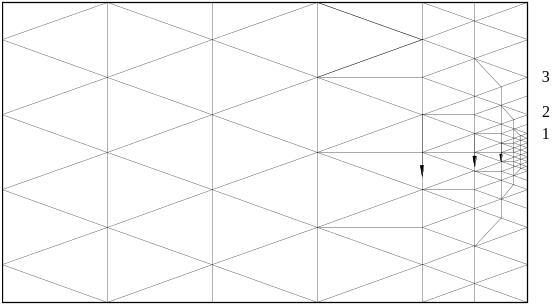
\includegraphics[width=0.8\textwidth]{assets/1134}
	\caption*{}
\end{figure}

{\bfseries Рис. 1 - Дискретная модель для 1/2 части образца с одной краевой
трещиной}

Следует обратить внимание на контуры интегрирования, которые обозначены
на этом рисунке 2. Задача решалась по двум расчетным схемам: плоская
деформация (ПД) и плоское напряженное состояние (ПНС), на основе теории
течения. В качестве материала рассмотрена сталь с параметрами:
\begin{figure}[H]
	\centering
	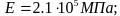
\includegraphics[width=0.8\textwidth]{assets/1135}
	\caption*{}
\end{figure} \begin{figure}[H]
	\centering
	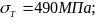
\includegraphics[width=0.8\textwidth]{assets/1136}
	\caption*{}
\end{figure}
\begin{figure}[H]
	\centering
	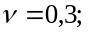
\includegraphics[width=0.8\textwidth]{assets/1137}
	\caption*{}
\end{figure} \begin{figure}[H]
	\centering
	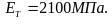
\includegraphics[width=0.8\textwidth]{assets/1138}
	\caption*{}
\end{figure}

Сравнение значений \begin{figure}[H]
	\centering
	
\includegraphics[width=0.8\textwidth]{assets/1139}
	\caption*{}
\end{figure}-интеграла при
решении упругопластической и упругой задач показано на рисунке 2 и 3. В
работе {[}9{]} показано, что линейная механика разрушения может
применяться вплоть до нетто-напряжения
\begin{figure}[H]
	\centering
	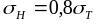
\includegraphics[width=0.8\textwidth]{assets/1140}
	\caption*{}
\end{figure} для краевых трещин в массивных телах
глубиной менее 0,25 сечения или для поверхностных трещин размером менее
половины сечения. Анализ полученных результатов показал, что пределы
применимости линейного подхода сильно зависят от степени стеснения
деформации, размеров дефектов и уровня напряжения в нетто-сечении. Так
для краевой трещины в случае плоского напряженного состояния с ошибкой в
15\% для трещин \begin{figure}[H]
	\centering
	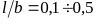
\includegraphics[width=0.8\textwidth]{assets/1141}
	\caption*{}
\end{figure} величина границы
применимости линейной механики разрушения изменяется в пределах
\begin{figure}[H]
	\centering
	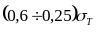
\includegraphics[width=0.8\textwidth]{assets/1142}
	\caption*{}
\end{figure} соответственно.

Для этих же трещин в условиях плоской деформации этот параметр
изменяется от \begin{figure}[H]
	\centering
	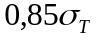
\includegraphics[width=0.8\textwidth]{assets/1143}
	\caption*{}
\end{figure} до
\begin{figure}[H]
	\centering
	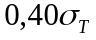
\includegraphics[width=0.8\textwidth]{assets/1144}
	\caption*{}
\end{figure}. По аналогии для образцов с
центральной трещиной получено, что для трещин длиной
\begin{figure}[H]
	\centering
	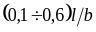
\includegraphics[width=0.8\textwidth]{assets/1145}
	\caption*{}
\end{figure} в случае плоского напряженного
состояния граница применимости линейного подхода оценивается как
\begin{figure}[H]
	\centering
	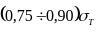
\includegraphics[width=0.8\textwidth]{assets/1146}
	\caption*{}
\end{figure}, а для плоской деформации -
\begin{figure}[H]
	\centering
	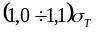
\includegraphics[width=0.8\textwidth]{assets/1147}
	\caption*{}
\end{figure}. Эти данные существенно уточняют
ранее полученные результаты других исследователей {[}6{]}.

\begin{figure}[H]
	\centering
	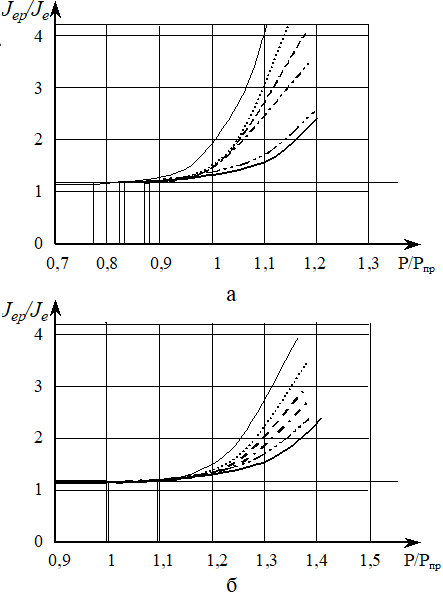
\includegraphics[width=0.8\textwidth]{assets/1148}
	\caption*{}
\end{figure}

{\bfseries Рис. 2 - Графики зависимости}
\begin{figure}[H]
	\centering
	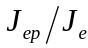
\includegraphics[width=0.8\textwidth]{assets/1149}
	\caption*{}
\end{figure} {\bfseries от приложенной нагрузки в
образце с центральной трещиной:} \emph{а -- плоское напряженное
состояние; б -- плоская деформация}

\begin{figure}[H]
	\centering
	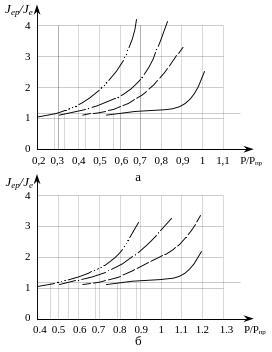
\includegraphics[width=0.8\textwidth]{assets/1150}
	\caption*{}
\end{figure}

{\bfseries Рис. 3 - Графики зависимости}
\begin{figure}[H]
	\centering
	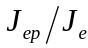
\includegraphics[width=0.8\textwidth]{assets/1151}
	\caption*{}
\end{figure} {\bfseries от приложенной нагрузки в
образце с краевой трещиной:}\\
\emph{а -- плоское напряженное состояние; б -- плоская деформация}

Сказанное выше позволяет перейти к определению аналитических
зависимостей \begin{figure}[H]
	\centering
	
\includegraphics[width=0.8\textwidth]{assets/1152}
	\caption*{}
\end{figure}-интеграла в функции
приложенного напряжения, геометрии элемента конструкции с трещиной и
свойств материала. В ряде работ {[}7, 8{]} предложены такие зависимости
в виде:

\begin{figure}[H]
	\centering
	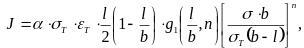
\includegraphics[width=0.8\textwidth]{assets/1153}
	\caption*{}
\end{figure} (1)

где g\textsubscript{1} - функция отношения длины трещины \emph{l} к
ширине пластины \emph{b} и показателя упрочнения материала n. При этом
предполагается, что материал упрочняется по степенному закону:

\begin{figure}[H]
	\centering
	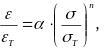
\includegraphics[width=0.8\textwidth]{assets/1154}
	\caption*{}
\end{figure} (2)

где α - константа материала, \begin{figure}[H]
	\centering
	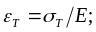
\includegraphics[width=0.8\textwidth]{assets/1155}
	\caption*{}
\end{figure} функция
\begin{figure}[H]
	\centering
	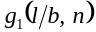
\includegraphics[width=0.8\textwidth]{assets/1156}
	\caption*{}
\end{figure} приводится в табулированном виде
{[}8{]}.

Анализ выражения (1) позволяет заключить, что параметр
\begin{figure}[H]
	\centering
	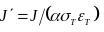
\includegraphics[width=0.8\textwidth]{assets/1157}
	\caption*{}
\end{figure} зависит только от относительной
длины трещины, приложенной нагрузки и показателя упрочнения \emph{n}.
Так в работе {[}8{]} приведены табулированные значения функции
\begin{figure}[H]
	\centering
	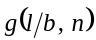
\includegraphics[width=0.8\textwidth]{assets/1158}
	\caption*{}
\end{figure} для образцов с центральной трещиной
для случая плоской деформации. Установить подобное выражение для других
расчетных случаев, характерных для сварных соединений с
непроплавлениями, можно на основе МКЭ и численного эксперимента.

Сказанное выше, распространим на материалы, упрочняющиеся по билинейному
закону. В этом случае, из рассмотрения можно исключить параметр
\emph{n=1.} На основе численного эксперимента было установлено, что
параметр \begin{figure}[H]
	\centering
	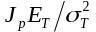
\includegraphics[width=0.8\textwidth]{assets/1159}
	\caption*{}
\end{figure} не зависит от материала при
развитых пластических деформациях, когда напряжения в нетто-сечении
образца \begin{figure}[H]
	\centering
	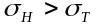
\includegraphics[width=0.8\textwidth]{assets/1160}
	\caption*{}
\end{figure}. Здесь
\begin{figure}[H]
	\centering
	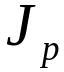
\includegraphics[width=0.8\textwidth]{assets/1161}
	\caption*{}
\end{figure}- пластический
\begin{figure}[H]
	\centering
	
\includegraphics[width=0.8\textwidth]{assets/1162}
	\caption*{}
\end{figure}- интеграл, определяемый как

\begin{figure}[H]
	\centering
	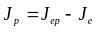
\includegraphics[width=0.8\textwidth]{assets/1163}
	\caption*{}
\end{figure}, (3)

где\begin{figure}[H]
	\centering
	
\includegraphics[width=0.8\textwidth]{assets/1164}
	\caption*{}
\end{figure}- упругий
\begin{figure}[H]
	\centering
	
\includegraphics[width=0.8\textwidth]{assets/1165}
	\caption*{}
\end{figure} - интеграл;
\begin{figure}[H]
	\centering
	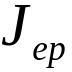
\includegraphics[width=0.8\textwidth]{assets/1166}
	\caption*{}
\end{figure}-упругопластический
\begin{figure}[H]
	\centering
	
\includegraphics[width=0.8\textwidth]{assets/1167}
	\caption*{}
\end{figure}- интеграл.

С учетом сказанного можно записать

\begin{figure}[H]
	\centering
	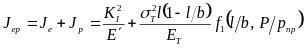
\includegraphics[width=0.8\textwidth]{assets/1168}
	\caption*{}
\end{figure}, (4)

где \begin{figure}[H]
	\centering
	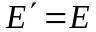
\includegraphics[width=0.8\textwidth]{assets/1169}
	\caption*{}
\end{figure}в случае плоско напряженного
состояния; \begin{figure}[H]
	\centering
	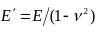
\includegraphics[width=0.8\textwidth]{assets/1170}
	\caption*{}
\end{figure}в случае плоской
деформации; \begin{figure}[H]
	\centering
	\includegraphics[width=0.8\textwidth]{assets/1171}
	\caption*{}
\end{figure}- некоторая функция,
зависящая от относительной длины трещины и уровня приложенной нагрузки.

В выражении (4) величина

\begin{figure}[H]
	\centering
	\includegraphics[width=0.8\textwidth]{assets/1172}
	\caption*{}
\end{figure}.

Используя уравнения для \begin{figure}[H]
	\centering
	\includegraphics[width=0.8\textwidth]{assets/1173}
	\caption*{}
\end{figure}{[}9{]},
записанные в общем виде, выражение (4) можно представить в виде

\begin{figure}[H]
	\centering
	\includegraphics[width=0.8\textwidth]{assets/1174}
	\caption*{}
\end{figure}. (5)

Появление сомножителя (\begin{figure}[H]
	\centering
	\includegraphics[width=0.8\textwidth]{assets/1175}
	\caption*{}
\end{figure}) связано с
необходимостью удовлетворения выражений (4) и (5) граничным условиям
задачи.

На основе численного эксперимента получены табулированные значения для
функции \begin{figure}[H]
	\centering
	\includegraphics[width=0.8\textwidth]{assets/1176}
	\caption*{}
\end{figure}. На рисунках 4 и 5
представлены графические зависимости параметра
\begin{figure}[H]
	\centering
	\includegraphics[width=0.8\textwidth]{assets/1177}
	\caption*{}
\end{figure} от длины трещины и приложенной
нагрузки.

На рисунке 6 приведены результаты расчета на основе табулированных
данных для \begin{figure}[H]
	\centering
	\includegraphics[width=0.8\textwidth]{assets/1178}
	\caption*{}
\end{figure}- интеграла (ПНС) в
образце с центральной трещиной зависимости разрушающих напряжений
\begin{figure}[H]
	\centering
	\includegraphics[width=0.8\textwidth]{assets/1179}
	\caption*{}
\end{figure} от относительной длины трещины
\begin{figure}[H]
	\centering
	\includegraphics[width=0.8\textwidth]{assets/1180}
	\caption*{}
\end{figure}. Расчетные значения хорошо
согласуются с экспериментальными {[}7{]} и уменьшаются с увеличением
длины трещины. Рассматривалась пластина из нержавеющей стали 1X18H9T
(\begin{figure}[H]
	\centering
	\includegraphics[width=0.8\textwidth]{assets/1181}
	\caption*{}
\end{figure}\begin{figure}[H]
	\centering
	\includegraphics[width=0.8\textwidth]{assets/1182}
	\caption*{}
\end{figure}\begin{figure}[H]
	\centering
	\includegraphics[width=0.8\textwidth]{assets/1183}
	\caption*{}
\end{figure}).
Увеличение ширины пластины также приводит к снижению разрушающих
напряжений, причем для пластин с центральной трещиной шириной
\begin{figure}[H]
	\centering
	\includegraphics[width=0.8\textwidth]{assets/1184}
	\caption*{}
\end{figure} напряжения σ\textsubscript{С}
оказались меньше предела текучести материала
\begin{figure}[H]
	\centering
	\includegraphics[width=0.8\textwidth]{assets/1185}
	\caption*{}
\end{figure}. В пластине с краевой трещиной такая
ситуация наблюдается уже в пластинах шириной
\begin{figure}[H]
	\centering
	\includegraphics[width=0.8\textwidth]{assets/1186}
	\caption*{}
\end{figure} \begin{figure}[H]
	\centering
	\includegraphics[width=0.8\textwidth]{assets/1187}
	\caption*{}
\end{figure}.

\begin{figure}[H]
	\centering
	\includegraphics[width=0.8\textwidth]{assets/1188}
	\caption*{}
\end{figure}

{\bfseries Рисунок 4 -Зависимость параметра}
\begin{figure}[H]
	\centering
	\includegraphics[width=0.8\textwidth]{assets/1189}
	\caption*{}
\end{figure} {\bfseries для образца с центральной
трещиной (100x200 мм):}\\
1 -- плоская деформация; 2 --плоское напряженное
состояние;\emph{P/P\textsubscript{пр}} =1,4

\begin{figure}[H]
	\centering
	\includegraphics[width=0.8\textwidth]{assets/1190}
	\caption*{}
\end{figure}

{\bfseries Рис. 5 - Зависимость параметра}
\begin{figure}[H]
	\centering
	\includegraphics[width=0.8\textwidth]{assets/1191}
	\caption*{}
\end{figure} {\bfseries для образца с краевой
трещиной (100x200 мм}):

\emph{1 -- плоская деформация; 2 --плоское напряженное состояние;
P/P\textsubscript{пр} =1,4}

Можно заключить, что для исследуемой стали расчет по предложенной
формуле дает удовлетворительную погрешность (≈5\%).

\begin{figure}[H]
	\centering
	\includegraphics[width=0.8\textwidth]{assets/1192}
	\caption*{}
\end{figure}

{\bfseries Рис. 6 -Зависимость параметра}
\begin{figure}[H]
	\centering
	\includegraphics[width=0.8\textwidth]{assets/1193}
	\caption*{}
\end{figure} {\bfseries от относительной длины
трещины} \begin{figure}[H]
	\centering
	\includegraphics[width=0.8\textwidth]{assets/1194}
	\caption*{}
\end{figure}:\\
\emph{1 -- b=70 мм; 2 -- b=150 мм; 3 -- b=300 мм; 4 -- b=600 мм; • -
экспериментальные данные} \emph{{[}7{]}}

{\bfseries Результаты и обсуждения.} Для высокопластичных материалов с
трещинами и вязким характером разрушения, если даже момент страгивания
установлен критерием \begin{figure}[H]
	\centering
	\includegraphics[width=0.8\textwidth]{assets/1195}
	\caption*{}
\end{figure}, необходимо
решить задачу распространении трещины, так как характер роста трещины
(устойчивое или неустойчивое) может существенно влиять на
работоспособность и ресурс конструкции. В качестве характеристики
сопротивления материала росту трещины используют
\begin{figure}[H]
	\centering
	\includegraphics[width=0.8\textwidth]{assets/1196}
	\caption*{}
\end{figure}-кривые {[}10{]}, определяемые
экспериментально. Эти кривые связывают значения
\begin{figure}[H]
	\centering
	\includegraphics[width=0.8\textwidth]{assets/1197}
	\caption*{}
\end{figure}-интеграла с приращением длины
трещины \begin{figure}[H]
	\centering
	\includegraphics[width=0.8\textwidth]{assets/1198}
	\caption*{}
\end{figure}. Переход к неустойчивому
распространению трещины будет иметь место, если в точке касания
\begin{figure}[H]
	\centering
	\includegraphics[width=0.8\textwidth]{assets/1199}
	\caption*{}
\end{figure} и
\begin{figure}[H]
	\centering
	\includegraphics[width=0.8\textwidth]{assets/1200}
	\caption*{}
\end{figure}-кривой выполняются условия

\begin{figure}[H]
	\centering
	\includegraphics[width=0.8\textwidth]{assets/1201}
	\caption*{}
\end{figure} и
\begin{figure}[H]
	\centering
	\includegraphics[width=0.8\textwidth]{assets/1202}
	\caption*{}
\end{figure}, (6)

Расчет J- кривой (рисунок 7) для стальной пластины с центральной
трещиной проводили по данным {[}9{]} для пластины с центральной
трещиной. \begin{figure}[H]
	\centering
	\includegraphics[width=0.8\textwidth]{assets/1203}
	\caption*{}
\end{figure}-кривая построена по
данным, полученным с помощью метода делительных сеток {[}7{]}.

\begin{figure}[H]
	\centering
	\includegraphics[width=0.8\textwidth]{assets/1204}
	\caption*{}
\end{figure}

{\bfseries Рис. 7 -} \begin{figure}[H]
	\centering
	\includegraphics[width=0.8\textwidth]{assets/1205}
	\caption*{}
\end{figure} {\bfseries и}
\begin{figure}[H]
	\centering
	\includegraphics[width=0.8\textwidth]{assets/1206}
	\caption*{}
\end{figure} {\bfseries -- кривые для образца с
центральной трещиной для стали 1Х18H9T}

{\bfseries (}\begin{figure}[H]
	\centering
	\includegraphics[width=0.8\textwidth]{assets/1207}
	\caption*{}
\end{figure}{\bfseries =70 мм;}
\begin{figure}[H]
	\centering
	\includegraphics[width=0.8\textwidth]{assets/1208}
	\caption*{}
\end{figure}{\bfseries =0,5)}

Из сопоставления приведенных J и J\textsubscript{R}-кривых (рисунок 7)
следует, что неустойчивое распространение трещины в пластине заданных
размеров в соответствии с условием (6) будет иметь место лишь при
заданной нагрузке. Переход к неустойчивому распространению трещины
произойдет при напряжении σ=236МПа после увеличения трещины на
\begin{figure}[H]
	\centering
	\includegraphics[width=0.8\textwidth]{assets/1209}
	\caption*{}
\end{figure} (для сравнения
\begin{figure}[H]
	\centering
	\includegraphics[width=0.8\textwidth]{assets/1210}
	\caption*{}
\end{figure}) {[}7{]}.

Представленные данные дают хорошее совпадение с исследованиями других
авторов и в отличие от них являются универсальными для рассматриваемых
классов сталей и законов упрочнения материалов.

Таким образом, зная вязкость разрушения
\begin{figure}[H]
	\centering
	\includegraphics[width=0.8\textwidth]{assets/1211}
	\caption*{}
\end{figure}, свойства материала, геометрию
элементов конструкции и ее НДС, можно определить предельную нагрузку,
при которой трещина начнет распространяться.

На основе предложенного в работе подхода {[}9{]} рассмотрим влияние
остаточных сварочных напряжений на величину
\begin{figure}[H]
	\centering
	\includegraphics[width=0.8\textwidth]{assets/1212}
	\caption*{}
\end{figure}- интеграла. В данном случае решается
задача расчета \begin{figure}[H]
	\centering
	\includegraphics[width=0.8\textwidth]{assets/1213}
	\caption*{}
\end{figure}- интеграла в образце
с центральной трещиной при совместном действии внешней нагрузки
\begin{figure}[H]
	\centering
	\includegraphics[width=0.8\textwidth]{assets/1214}
	\caption*{}
\end{figure}и нагрузки на берегах трещины,
эквивалентной действию остаточных напряжений. Рассматривалась пластина
размерами 100x200 мм из Ст3 со следующими характеристиками:
\begin{figure}[H]
	\centering
	\includegraphics[width=0.8\textwidth]{assets/1215}
	\caption*{}
\end{figure} \begin{figure}[H]
	\centering
	\includegraphics[width=0.8\textwidth]{assets/1216}
	\caption*{}
\end{figure}
\begin{figure}[H]
	\centering
	\includegraphics[width=0.8\textwidth]{assets/1217}
	\caption*{}
\end{figure}. В качестве варьируемых параметров
использовались: \begin{figure}[H]
	\centering
	\includegraphics[width=0.8\textwidth]{assets/1218}
	\caption*{}
\end{figure}- относительная длина
трещины; \begin{figure}[H]
	\centering
	\includegraphics[width=0.8\textwidth]{assets/1219}
	\caption*{}
\end{figure}-приложенная относительная
внешняя нагрузка; \begin{figure}[H]
	\centering
	\includegraphics[width=0.8\textwidth]{assets/1220}
	\caption*{}
\end{figure}- отношение
нерелаксированных остаточных напряжений к пределу текучести материала. В
результате численного эксперимента оценивались значения функции

\begin{figure}[H]
	\centering
	\includegraphics[width=0.8\textwidth]{assets/1221}
	\caption*{}
\end{figure}, (7)

где \begin{figure}[H]
	\centering
	\includegraphics[width=0.8\textwidth]{assets/1222}
	\caption*{}
\end{figure}энергетический
\begin{figure}[H]
	\centering
	\includegraphics[width=0.8\textwidth]{assets/1223}
	\caption*{}
\end{figure} - интеграл от внешней нагрузки;
\begin{figure}[H]
	\centering
	\includegraphics[width=0.8\textwidth]{assets/1224}
	\caption*{}
\end{figure}- энергетический
\begin{figure}[H]
	\centering
	\includegraphics[width=0.8\textwidth]{assets/1225}
	\caption*{}
\end{figure} - интеграл от внешней нагрузки и
нерелаксированных остаточных напряжений.

Предыдущие исследования позволяют принять с некоторой долей приближения,
что функция \begin{figure}[H]
	\centering
	\includegraphics[width=0.8\textwidth]{assets/1226}
	\caption*{}
\end{figure} не зависит от материала
образца. Были приняты следующие диапазоны изменения факторов:
\begin{figure}[H]
	\centering
	\includegraphics[width=0.8\textwidth]{assets/1227}
	\caption*{}
\end{figure};
\begin{figure}[H]
	\centering
	\includegraphics[width=0.8\textwidth]{assets/1228}
	\caption*{}
\end{figure};
\begin{figure}[H]
	\centering
	\includegraphics[width=0.8\textwidth]{assets/1229}
	\caption*{}
\end{figure}. При этом учитывалось допустимое
сочетание остаточных и приложенных напряжений.

На рисунках 8 и 9 представлены некоторые результаты численного
моделирования. Влияние остаточных напряжений на величину функции
\begin{figure}[H]
	\centering
	\includegraphics[width=0.8\textwidth]{assets/1230}
	\caption*{}
\end{figure} усиливается с ростом длины трещины
и увеличением внешней нагрузки (см. рис.8,
\begin{figure}[H]
	\centering
	\includegraphics[width=0.8\textwidth]{assets/1231}
	\caption*{}
\end{figure}МПа и
\begin{figure}[H]
	\centering
	\includegraphics[width=0.8\textwidth]{assets/1232}
	\caption*{}
\end{figure}МПа). При больших значениях
приложенных напряжений (рис.9) растягивающие остаточные напряжения
релаксируют и почти не оказывают влияния на величину
\begin{figure}[H]
	\centering
	\includegraphics[width=0.8\textwidth]{assets/1233}
	\caption*{}
\end{figure}{\bfseries -}интеграла. С понижением
\begin{figure}[H]
	\centering
	\includegraphics[width=0.8\textwidth]{assets/1234}
	\caption*{}
\end{figure} влияние остаточных напряжений
становится более заметно. Так, если вязкость разрушения
\begin{figure}[H]
	\centering
	\includegraphics[width=0.8\textwidth]{assets/1235}
	\caption*{}
\end{figure}{\bfseries ,} то прочность соединения
уменьшается на 19\% \begin{figure}[H]
	\centering
	\includegraphics[width=0.8\textwidth]{assets/1236}
	\caption*{}
\end{figure} за счет
действия нерелаксированных остаточных напряжений. Приведенные данные
свидетельствуют о существенном влиянии остаточных напряжений на
трещиностойкость элементов металлоконструкций, что согласуется с данными
эксперимента {[}9{]}.

\begin{figure}[H]
	\centering
	\includegraphics[width=0.8\textwidth]{assets/1237}
	\caption*{}
\end{figure}

{\bfseries Рис. 8 - Зависимость функции}
\begin{figure}[H]
	\centering
	\includegraphics[width=0.8\textwidth]{assets/1238}
	\caption*{}
\end{figure} {\bfseries от длины трещины,
остаточных} \begin{figure}[H]
	\centering
	\includegraphics[width=0.8\textwidth]{assets/1239}
	\caption*{}
\end{figure} {\bfseries и внешних}
\begin{figure}[H]
	\centering
	\includegraphics[width=0.8\textwidth]{assets/1240}
	\caption*{}
\end{figure} {\bfseries напряжений}

Значение функции \begin{figure}[H]
	\centering
	\includegraphics[width=0.8\textwidth]{assets/1241}
	\caption*{}
\end{figure} приведено в работе
{[}9{]} в табулированном виде. На основе описанного подхода можно
получить подобные функции и для других типов сварных соединений.

Таким образом, зная уровень нерелаксированных остаточных напряжений,
размер дефекта и используя табулированную функцию
\begin{figure}[H]
	\centering
	\includegraphics[width=0.8\textwidth]{assets/1242}
	\caption*{}
\end{figure}, можно оценить величину
\begin{figure}[H]
	\centering
	\includegraphics[width=0.8\textwidth]{assets/1243}
	\caption*{}
\end{figure}{\bfseries -}интеграла в виде

\begin{figure}[H]
	\centering
	\includegraphics[width=0.8\textwidth]{assets/1244}
	\caption*{}
\end{figure} (8)

\begin{figure}[H]
	\centering
	\includegraphics[width=0.8\textwidth]{assets/1245}
	\caption*{}
\end{figure}

{\bfseries Рис. 9 - Влияние нерелаксированных остаточных напряжений на
величину \emph{J}-интеграла}

Здесь значение \begin{figure}[H]
	\centering
	\includegraphics[width=0.8\textwidth]{assets/1246}
	\caption*{}
\end{figure}{\bfseries -}интеграла
от действия внешней нагрузки и длины трещины определяем на основе
табулированных данных {[}9{]}.

{\bfseries Выводы.} В данной работе с помощью полученных регрессионых
зависимостей решены следующие задачи.

Определены границы применяемости линейной механики разрушения для
краевых и центральных трещин в типичных образцах.

Установлены зависимости разрушающих напряжений
\begin{figure}[H]
	\centering
	\includegraphics[width=0.8\textwidth]{assets/1247}
	\caption*{}
\end{figure} от относительной длины трещины
\begin{figure}[H]
	\centering
	\includegraphics[width=0.8\textwidth]{assets/1248}
	\caption*{}
\end{figure} в образцах с центральной и краевой
трещинами на основе \begin{figure}[H]
	\centering
	\includegraphics[width=0.8\textwidth]{assets/1249}
	\caption*{}
\end{figure}-интеграла.

Оценено влияние остаточных напряжений на величину \emph{J}-интеграла в
типовых образцах.

Таким образом, регрессионные зависимости для определения
\emph{J}-интеграла обладают достаточной надежностью и могут
использоваться в практике прогнозирования остаточного ресурса сварных
металлоконструкций.

{\bfseries Литература}

1. Richard, H., Sander, M., Fulland, M. and Kullmer, G. Development of
fatigue crack growth in real structures // Engineering Fracture
Mechanics. - 2008. -- Vol. 75. - P. 331-340. DOI
10.1016/j.engfracmech.2007.01.017

2. Ghosh A., Barman N., Chattopadhyay H., Hloch S. A study of thermal
behaviour during submerged arc welding.// J Mech Eng.- 2013.- Vol.
59(5)- P. 333-338. DOI 10.5545/sv-jme.2012.775

3. Zhu M.-L., Xuan F.-Z. and Tu S.-T. Effect of load ratio on fatigue
crack growth in the near-threshold regime: A literature review, and a
combined crack closure and driving force approach//Engineering Fracture
Mechanics.- 2015.- Vol. 141.- P. 57-77. DOI
10.1016/j.engfracmech.2015.05.005

4. Besel, M. and Breitbarth, E. Advanced analysis of crack tip plastic
zone under cyclic loading// International Journal of Fatigue. -2016. -
Vol. 93(1).-P. 92-108. DOI 10.1016/j.ijfatigue.2016.08.013

5. Lopez-Crespo, P., Shterenlikht, A., Patterson, E. A., Yates, J. R.
and Withers, P. J. The stress intensity of mixed mode cracks determined
by digital image correlation // Journal of strain analsysis for
engineering design.-2008. -Vol. 43. - P. 769-780. DOI
10.1243/03093247JSA419

6. Нұрғожин М.Р., Даненова Г.Т., Сайлауқызы Ж.Қалдық дәнекерлеу
кернеулеріне және деформацияға механикалық әсердің әсерін компьютерлік
модельдеу // Университ Еңбектері ҚарМТУ.-2020-№ 3(80).-С.19-24. DOI
10.25209/1609- 1825\_2020\_3\_19

7. Nurguzhin M., Danenova G., Akhmetzhanov T. Computer modeling of the
stress-strain state of welded construction// in AIP Conf Proc. -
Prospects of fundamental sciences development (PFSD-2017).- Tomsk.-
2017.- V.1899 (1). DOI 10.1063/1.5009879

8. Traidia A., Roger F. Numerical and experimental study of arc and weld
pool behavior for pulsed current GTA welding.// Int J Heat Mass Tran.-
2011.- Vol. 54 (9-10).- P.2163-2179. DOI
10.1016/j.ijheatmasstransfer.2010.12.005

9. Нургужин М.Р., Даненова Г.Т. Основы расчета характеристик живучести
сварных металлоконструкций: монография. - Караганда. Изд-во КарТУ.-
2021.- 133 с.

10. Нургужин М.Р., Даненова Г.Т. Моделирование тепловых процессов в
сварных соединениях: монография. -Караганда: Изд-во НАО «КарТУ имени
Абылкаса Сагинова».- 2023.- 83 с.

{\bfseries References}

1. Richard, H., Sander, M., Fulland, M. and Kullmer, G. Development of
fatigue crack growth in real structures // Engineering Fracture
Mechanics. - 2008. -- Vol. 75. - P. 331-340. DOI
10.1016/j.engfracmech.2007.01.017

2. Ghosh A., Barman N., Chattopadhyay H., Hloch S. A study of thermal
behaviour during submerged arc welding.// J Mech Eng.- 2013.- Vol.
59(5)- P. 333-338. DOI 10.5545/sv-jme.2012.775

3. Zhu M.-L., Xuan F.-Z. and Tu S.-T. Effect of load ratio on fatigue
crack growth in the near-threshold regime: A literature review, and a
combined crack closure and driving force approach//Engineering Fracture
Mechanics.- 2015.- Vol. 141.- P. 57-77. DOI
10.1016/j.engfracmech.2015.05.005

4. Besel, M. and Breitbarth, E. Advanced analysis of crack tip plastic
zone under cyclic loading// International Journal of Fatigue. -2016. -
Vol. 93(1).-P. 92-108. DOI 10.1016/j.ijfatigue.2016.08.013

5. Lopez-Crespo, P., Shterenlikht, A., Patterson, E. A., Yates, J. R.
and Withers, P. J. The stress intensity of mixed mode cracks determined
by digital image correlation // Journal of strain analsysis for
engineering design.-2008. -Vol. 43. - P. 769-780. DOI
10.1243/03093247JSA419

6. Nūrğojin M.R., Danenova G.T., SailauqyzyJ.Qaldyq dänekerleu
kerneulerıne jäne deformasiağa mehanikalyq äserdıñ äserın kömpüterlık
modeldeu // Universit Eñbekterı QarMTU.-2020-№ 3(80).-S.19-24. DOI
10.25209/1609- 1825\_2020\_3\_19 {[}in Kazakh{]}

7. Nurguzhin M., Danenova G., Akhmetzhanov T. Computer modeling of the
stress-strain state of welded construction// in AIP Conf Proc. -
Prospects of fundamental sciences development (PFSD-2017).- Tomsk.-
2017.- V.1899 (1). DOI 10.1063/1.5009879

8. Traidia A., Roger F. Numerical and experimental study of arc and weld
pool behavior for pulsed current GTA welding.// Int J Heat Mass Tran.-
2011.- Vol. 54 (9-10).- P.2163-2179. DOI
10.1016/j.ijheatmasstransfer.2010.12.005

9. Nurguzhin M.R., Danenova G.T. Osnovy rascheta kharakteristik
zhivuchesti svarnykh metallokonstruktsii: monografiya. - Karaganda.
Izd-vo KarTU.- 2021.- 133 s. {[}in Russian{]}

10. Nurguzhin M.R., Danenova G.T. Modelirovanie teplovykh protsessov v
svarnykh soedineniyakh: monografiya. -Karaganda: Izd-vo NAO «KarTU imeni
Abylkasa Saginova».- 2023.- 83 s. {[}in Russian{]}

\emph{{\bfseries Сведения об авторах}}

Нургужин М.Р. - доктор технических наук, профессор, Акционерное общество
«Национальный центр космических исследований и технологий», Алматы,
Казахстан, e-mail: maratnurg57@mail.ru;

Даненова Г.Т. - кандидат технических наук, доцент, Карагандинский
технический университет имени Абылкаса Сагинова, Караганда, Казахстан,
e-mail: guldan72@mail.ru;

Нургужина А.М. - кандидат технических наук, доцент, Astana IT
университет, Астана, Казахстан, e-mail:
assel.nurguzhina@astanait.edu.kz;

Ахметжанов Т.Б. -кандидат технических наук, доцент, Карагандинский
технический университет имени Абылкаса Сагинова, Караганда, Казахстан,
e-mail: akhmetzhantalgat@gmail.com

\emph{{\bfseries Information about the authors}}

Nurguzhin M.R. - Doctor of Technical Sciences, Professor, Joint Stock
Company ``National Center of Space Researches and Technologies'',
Almaty, Kazakhstan, e-mail: maratnurg57@mail.ru;

Danenova G.T. - Сandidate of Technical Sciences, Associate Professor,
Karaganda Technical University named by Abylkas Saginov, Karaganda,
Kazakhstan, e-mail: guldan72@mail.ru;

Nurguzhinа А.M. - Сandidate of Technical Sciences, Associate Professor,
Astana IT University, Astana, Kazakhstan, e-mail:
assel.nurguzhina@astanait.edu.kz;

Akhmetzhanov T.B. - Сandidate of Technical Sciences, Associate
Professor, Karaganda Technical University named by Abylkas Saginov,
Karaganda, Kazakhstan, e-mail: akhmetzhantalgat@gmail.com\newpage
{\bfseries ҒТАМР 84.13.21}

{\bfseries МҰНАЙ-ГАЗ КЕШЕНІ КӘСІПОРЫНДАРЫНДА САПА МЕНЕДЖМЕНТІ ЖҮЙЕСІН
ҚАЛЫПТАСТЫРУ ЖӘНЕ ДАМЫТУ}

{\bfseries Г.К. Тайманова, Б.Б. Заутбек\textsuperscript{🖂}}

Әл-Фараби атындағы Қазақ ұлттық университеті, Алматы, Қазақстан,

{\bfseries \textsuperscript{🖂}}Корреспондент-автор:
balzhan.zautbek02@gmail.com

Саланың қарқынды дамуы жағдайында сапаны тиімді басқару осы сектор
кәсіпорындарының табысты қызметінің маңызды элементіне айналады. Мақала
сапа менеджменті жүйесін қалыптастырудың негізгі аспектілерін анықтауға,
сондай-ақ, мұнай-газ саласының ерекшелігін ескере отырып, оны дамыту
әдістерін зерттеуге бағытталған.

Мақалада сапа менеджменті жүйесінің негізгі принциптері, ISO 9001:2015,
OHSAS 18001:2008, ISO 14001:2015 және ISO 45001:2018 және т.б.
стандарттары, сондай-ақ, мұнай-газ секторына тән нақты талаптар
қарастырылады. Мұнай-газ кешені кәсіпорындарында сапаны басқару
жүйелерін енгізудің табысты тәжірибелері талданады, сондай-ақ, осы
процесте компаниялардың алдында тұрған сын-қатерлер мен проблемалар
анықталады.

Мақалада мұнай-газ кешені кәсіпорындарында персоналды оқыту және сапа
мәдениетін дамыту мәселелері қарастырылады. Персоналды сапаны басқару
процестеріне тартудың және олардың рөлі жүйенің жалпы тиімділігіне қалай
әсер ететінін түсінуді қалыптастырудың маңыздылығына баса назар
аударылады.

Зерттеу барысында алынған тұжырымдар мұнай-газ кешені кәсіпорындарындағы
сапа менеджменті жүйесін одан әрі жетілдіруге құнды үлес болып табылады.
Энергетика секторындағы сапа менеджменті саласындағы болашақ зерттеулер
үшін негіз болады.

{\bfseries Түйін сөздер:} корпоративтік басқару, сапа менеджменті жүйелері,
SWOT-талдау, экологиялық көрсеткіштер, тиімділік, тұрақты жетілдіру.

{\bfseries ФОРМИРОВАНИЕ И РАЗВИТИЕ СИСТЕМЫ МЕНЕДЖМЕНТА КАЧЕСТВА НА
ПРЕДПРИЯТИЯХ НЕФТЕГАЗОВОГО КОМПЛЕКСА}

{\bfseries Г.К. Тайманова, Б.Б. Заутбек\textsuperscript{🖂}}

Казахский национальный~университет~имени Аль-Фараби, Алматы, Казахстан,

e-mail: balzhan.zautbek02@gmail.com

В условиях динамичного развития отрасли, эффективное управление
качеством становится критически важным элементом успешной деятельности
предприятий данного сектора. Статья направлена на выявление ключевых
аспектов формирования системы менеджмента качества, а также на
исследование методов её развития с учетом специфики нефтегазовой
отрасли.

В статье рассматриваются основные принципы системы менеджмента качества,
стандарты ISO~9001:2015, ISO~14001:2015 и~ISO~45001:2018 и др., а также
специфические требования, характерные для нефтегазового сектора.
Анализируются успешные практики внедрения систем управления качеством на
предприятиях нефтегазового комплекса, а также выявляются вызовы и
проблемы, с которыми сталкиваются компании в этом процессе.

В статье также рассматриваются вопросы обучения персонала и развития
культуры качества на предприятиях нефтегазового комплекса. Акцент
делается на важности вовлечения персонала в процессы управления
качеством и формирования понимания того, как их роль влияет на общую
результативность системы.

Полученные в ходе исследования выводы представляют собой ценный вклад в
дальнейшее совершенствование систем менеджмента качества на предприятиях
нефтегазового комплекса, а также служат основой для будущих исследований
в области управления качеством в энергетическом секторе.

{\bfseries Ключевые слова:} корпоративное управление, системы менеджмента
качества, SWOT-анализ, экологические показатели, эффективность,
постоянное совершенствование.

{\bfseries FORMATION AND DEVELOPMENT OF A QUALITY MANAGEMENT SYSTEM AT THE
ENTERPRISES OF THE OIL AND GAS COMPLEX}

{\bfseries G.K. Taimanova, B.B. Zautbek\textsuperscript{🖂}}

Al-Farabi Kazakh national university, Almaty, Kazakhstan,

e-mail: balzhan.zautbek02@gmail.com

In the context of the dynamic development of the industry, effective
quality management is becoming a critical element of the successful
operation of enterprises in this sector. The article aims to identify
the key aspects of the formation of a quality management system, as well
as to study the methods of its development, taking into account the
specifics of the oil and gas industry.

The article discusses the basic principles of the quality management
system, ISO 9001:2015, ISO 14001:2015 and ISO 45001:2018 standards,
etc., as well as specific requirements specific to the oil and gas
sector. The successful practices of implementing quality management
systems at oil and gas enterprises are analyzed, as well as the
challenges and problems faced by companies in this process are
identified.

The article also discusses the issues of personnel training and the
development of a quality culture at oil and gas enterprises. The
emphasis is on the importance of involving personnel in quality
management processes and developing an understanding of how their role
affects the overall effectiveness of the system.

The findings obtained in the course of the study represent a valuable
contribution to the further improvement of quality management systems at
oil and gas enterprises, and also serve as a basis for future research
in the field of quality management in the energy sector.

{\bfseries Keywords:} corporate governance, quality management systems,
SWOT analysis, environmental performance, efficiency, continuous
improvement.

{\bfseries Кіріспе.} ҚР бюджеті мен төлем балансының басым бөлігін
қалыптастыра отырып, мұнай-газ өндіру саласы мемлекет ауқымында түйінді
және стратегиялық маңызды болып табылады. ҚР-дағы мұнай-газ саласы ел
аумағында және одан тыс жерлерде мұнай мен газды өндіруді, өңдеуді,
жеткізуді және өңдеуді қамтиды. Мұнай-газ өндіру кешені республика
бюджетін қалыптастыру үшін стратегиялық маңызды компонент болып
табылады, бұл сала кәсіпорындарындағы бизнес-процестерді жетілдіру және
оңтайландыру тұрғысынан көптеген зерттеулерге негізделген. Атап
айтқанда, СМЖ енгізуді американдық мұнай институтының (API) Specq1
талаптары негізінде жүзеге асырған жөн, өйткені мұндай жүйе бірден үш
стандарттың өлшемдерін қанағаттандырады: APISpecQ1, ISO/TS 29001:2010,
ISO 9001: 2008. Осылайша, кәсіпорын өзінің бәсекелестік қуатын арттырып
қана қоймай, кейіннен пайданы ұлғайта алады. Негізгі тұтынушылар
тарапынан қолдауды қалыптастырады {[}1{]}. Американдық мұнай
институтының сапа менеджменті жүйесінің API Specification Q2 талаптарына
сәйкес мұнай сервисі активтерін сертификаттау мұнай сервисі активтері
қызметтерінің сапасын API мұнай-газ саласындағы халықаралық
стандарттардың озық және дамыған практикасына сәйкестік деңгейіне дейін
арттыру мақсатында басталды. Мұнайдың дәлелденген қоры бойынша Қазақстан
әлемде 12-орында - 3.9 млрд тонна. Табиғи газ қоры 2.7 трлн текше метрді
құрайды -- әлемдегі 14 орын. Қазақстанның дәлелденген мұнай және
конденсат қорларын өндірудің ағымдағы деңгейінде 45 жылдан астам уақытқа
жеткілікті (1-кесте) {[}2{]}.

{\bfseries 1-кесте \emph{-} Елдер бойынша дәлелденген мұнай және конденсат
қорлары, млрд. тонна}

\begin{longtable}[]{@{}
  >{\raggedright\arraybackslash}p{(\columnwidth - 6\tabcolsep) * \real{0.3180}}
  >{\raggedright\arraybackslash}p{(\columnwidth - 6\tabcolsep) * \real{0.2124}}
  >{\raggedright\arraybackslash}p{(\columnwidth - 6\tabcolsep) * \real{0.2730}}
  >{\raggedright\arraybackslash}p{(\columnwidth - 6\tabcolsep) * \real{0.1966}}@{}}
\toprule\noalign{}
\begin{minipage}[b]{\linewidth}\raggedright
{\bfseries Мемлекеттер}
\end{minipage} & \begin{minipage}[b]{\linewidth}\raggedright
{\bfseries Дәлелденген мұнай қорлары, млрд. тонн.}
\end{minipage} & \begin{minipage}[b]{\linewidth}\raggedright
{\bfseries Жетістік деңгейі неше жыл, жыл}
\end{minipage} & \begin{minipage}[b]{\linewidth}\raggedright
{\bfseries Әлемдік қордан, \%}
\end{minipage} \\
\midrule\noalign{}
\endhead
\bottomrule\noalign{}
\endlastfoot
Венесуэла & 48 & 500 & 17,5 \\
Сауд Арабиясы & 40,9 & 73,6 & 17,2 \\
Канада & 27,1 & 89,4 & 9,7 \\
Иран & 21,7 & 139,8 & 9,1 \\
Ирак & 19,6 & 96,3 & 8,4 \\
Ресей & 14,8 & 27,6 & 6,2 \\
Кувейт & 14 & 103,2 & 5,9 \\
Біріккен Араб Әмірліктері & 13 & 73,1 & 5,6 \\
АҚШ & 8,2 & 11,4 & 4 \\
Ливия & 6,3 & 339,2 & 2,8 \\
Нигерия & 5,0 & 56,1 & 2,1 \\
{\bfseries Қазақстан} & {\bfseries 3,9} & {\bfseries 45,3} & {\bfseries 1,7} \\
Қытай & 3,5 & 18,2 & 1,5 \\
Катар & 2,6 & 38,1 & 1,5 \\
Бразилиа & 1,7 & 10,8 & 0,7 \\
Алжир & 1,5 & 25,0 & 0,7 \\
Ангола & 1,1 & 16,1 & 0,4 \\
Норвегия & 1,0 & 10,8 & 0,5 \\
Әзірбайжан & 1,0 & 26,7 & 0,4 \\
Мексика & 0,9 & 8,7 & 0,4 \\
\end{longtable}

Нарықта бәсекеге қабілеттілікті арттыру үшін компаниялар
бизнес-процестерді тиімді басқаруды жүзеге асыруы және сапа менеджменті
жүйесін (СМЖ) енгізуі қажет. Егер сапа менеджменті жүйесі қабылданған
халықаралық стандарттарға сәйкес келсе, кәсіпорынның қызметі тиімді деп
саналуы мүмкін. Сапа жүйесінің стандарттары мен сәйкестік критерийлерін
таңдау кәсіпорынның түпкі мақсатына байланысты және мүдделі тұлғалардың
пікірін ескере отырып жүзеге асырылады. Сапаны басқаруды стандарттаудан
бөлек қарастыруға болмайды, оның нормативтік базасы компанияларға сапаны
бағалауға, тексеру процедурасы мен критерийлерін белгілеуге мүмкіндік
береді {[}3{]}.

{\bfseries Материалдар мен әдістер.} Мұнай-газ компанияларында енгізілген
сапа менеджменті жүйелері бизнес-процестерді, өнім сапасын жетілдіруді
қамтамасыз етеді және кәсіпорындар қызметінің түпкілікті нәтижелеріне өз
әсерін тигізеді. Бұл зерттеудің өзектілігін негіздейді.

Мұнай-газ секторы тәуелсіз компаниялардың кешені болып табылады, олардың
қызметі құрылатын тауардың бүкіл өмірлік циклін қамтиды. Өмірлік циклдің
барлық кезеңдерін сапа менеджменті жүйесінің көмегімен бағалау және
бақылау қажет, арнайы рәсімге және алдын ала белгіленген бағалау
критерийлеріне сәйкес халықаралық сапа стандарттарын енгізу қажет.
RAEX-Europe тәуелсіз Еуропалық рейтингтік агенттігінің деректері бойынша
мұнай-газ өндіру саласындағы өнімді өткізу көлемі бойынша Қазақстанның
ірі компанияларының рейтингі жасалды (2-кесте) {[}4{]}.

{\bfseries 2-кесте - 2021-2022 жылдар кезеңінде ҚР-дағы мұнай және газ
өндіру бойынша ірі компаниялардың рейтингі}

\begin{longtable}[]{@{}
  >{\raggedright\arraybackslash}p{(\columnwidth - 6\tabcolsep) * \real{0.3330}}
  >{\raggedright\arraybackslash}p{(\columnwidth - 6\tabcolsep) * \real{0.2728}}
  >{\raggedright\arraybackslash}p{(\columnwidth - 6\tabcolsep) * \real{0.2459}}
  >{\raggedright\arraybackslash}p{(\columnwidth - 6\tabcolsep) * \real{0.1483}}@{}}
\toprule\noalign{}
\begin{minipage}[b]{\linewidth}\raggedright
Компания
\end{minipage} & \begin{minipage}[b]{\linewidth}\raggedright
2021 жылы іске асыру көлемі, млн тг.
\end{minipage} & \begin{minipage}[b]{\linewidth}\raggedright
2020 жылы іске асыру көлемі, млн тг.
\end{minipage} & \begin{minipage}[b]{\linewidth}\raggedright
Өсу қарқыны, \%
\end{minipage} \\
\midrule\noalign{}
\endhead
\bottomrule\noalign{}
\endlastfoot
"ҚазМұнайГаз" ҰК & 5838793 & 3624964 & 61 \\
Қарашығанақ Петролиум Оперейтинг Б. В. & 1461823 & 1073920 & 36 \\
North Caspian Operating Company N.V. & 3737330 & 1871516 & 100 \\
Nostrum (ТОО «Жаикмунай») & 83197 & 72654 & 15 \\
«Матен Петролеум» & 157686 & 92339 & 71 \\
\end{longtable}

«ҚазМұнайГаз» ҰК АҚ компаниясы ҚР-дағы мұнай-газ өндіру саласындағы
компаниялар тізімінің көшбасшысы болды. Мұнай-газ компаниясы қандай
стандарттарды қолданатынын қарастырайық. Кәсіпорындар құжаттаманы және
сапа стандарттарының көпшілігін дербес әзірлейді. 2006 жылдан бастап
ҚМГ-да ISO 9001:2015, OHSAS 18001:2018, ISO 14001:2015 және ISO
45001:2018 талаптарына сәйкес сапа, қоршаған ортаны қорғау, денсаулықты
қорғау және еңбек қауіпсіздігін қамтамасыз ету саласында басқарудың
интеграцияланған жүйесі енгізілді {[}5{]}. Энергия тұтынудың едәуір
деңгейі бар компания ISO 50001:2018 стандартына сәйкес сертификатталған.
Біріктірілген басқару жүйесінің тиімділігін тәуелсіз аудиторлар үнемі
растайды. Олар компания ішінде де, ол жұмыс істейтін кәсіпорындарда да
таралады {[}6{]}.

ҚМГ корпоративтік басқару жүйесі кәсіпорындардың қызметін басқару мен
бақылауды, сондай-ақ, акционерлер, Директорлар кеңесі, басқарма және
мүдделі тараптар арасындағы өзара қарым-қатынас жүйесін қамтамасыз
ететін процестердің жиынтығы болып табылады. 2015 жылдан бастап қазіргі
уақытқа дейін ҚМГ «Самұрық-Қазына» АҚ Басқармасының шешімімен бекітілген
ҚМГ корпоративтік басқару Кодексін енгізу бойынша жұмыс жүргізуде (2015
жылғы 27 мамырдағы №22/15 хаттама). ҚМГ корпоративтік басқару кодексінің
мақсаты корпоративтік басқаруды жетілдіру, басқарудың ашықтығын
қамтамасыз ету, ҚМГ-ның тиісті корпоративтік басқару стандарттарын
ұстануға бейілділігін растау болып табылады. Осылайша, ҚМГ-да
корпоративтік басқару құрылымы құрылады (1-сурет).

{\bfseries АКЦИОНЕРЛЕРДІҢ ЖАЛПЫ ЖИНАЛЫСЫ}

Тәуекелдер жөніндегі Комитет

ДИРЕКТОРЛАР КЕҢЕСІ

БАСҚАРМА

Корпоративтік хатшы

Омбудсмен

Сәйкестік қызметі

Тәуекелді басқару департаменті

Мақсат иелері

Тәуекел факторларының иелері

Тәуекел иелері

ІШКІ АУДИТ ҚЫЗМЕТІ

Қауіпсіздік, еңбекті қорғау, қоршаған орта және тұрақты даму комитеті

Аудит жөніндегі Комитет

Стратегия және портфельді басқару комитеті

Тағайындаулар және сыйақылар жөніндегі Комитет

{\bfseries 1-сурет - ҚМГ-дағы корпоративтік басқару құрылымы}

Тұтастай алғанда, компаниядағы корпоративтік басқаруды жетілдіру
үздіксіз циклдік процесс болып табылады, оның негізгі кезеңі тәуелсіз
тараптан рейтинг және жақсарту бойынша тиісті ұсыныстар алу болып
табылатындығының айқын көрінісін келесі 2-суреттен көре аламыз {[}7{]}.

{\bfseries 2-сурет - Корпоративтік басқару жүйесін дамыту}

2020-2022 жылдар кезеңінде «ҚазМұнайГаз» ҰК АҚ жұмыс тиімділігінің
көрсеткіштерінің өзгеру динамикасын қарастырайық (3-кесте). Кез келген
мұнай саласындағы компанияның көрсеткіштерінің өзгеру динамикасы мұнай
бағасына, сонымен қатар, мұнай өндіру, тасымалдау, т.б. процестерге
әсерін тигізеді {[}8{]}.

{\bfseries 3-кесте -- «ҚазМұнайГаз» ҰК АҚ-ның 2020-2022 жылдардағы
тиімділік көрсеткіштері}

\begin{longtable}[]{@{}
  >{\raggedright\arraybackslash}p{(\columnwidth - 6\tabcolsep) * \real{0.4545}}
  >{\raggedright\arraybackslash}p{(\columnwidth - 6\tabcolsep) * \real{0.1820}}
  >{\raggedright\arraybackslash}p{(\columnwidth - 6\tabcolsep) * \real{0.1820}}
  >{\raggedright\arraybackslash}p{(\columnwidth - 6\tabcolsep) * \real{0.1814}}@{}}
\toprule\noalign{}
\begin{minipage}[b]{\linewidth}\raggedright
Тиімділік көрсеткіші
\end{minipage} & \begin{minipage}[b]{\linewidth}\raggedright
2020
\end{minipage} & \begin{minipage}[b]{\linewidth}\raggedright
2021
\end{minipage} & \begin{minipage}[b]{\linewidth}\raggedright
2022
\end{minipage} \\
\midrule\noalign{}
\endhead
\bottomrule\noalign{}
\endlastfoot
Тұтынушылардың өндіруге, тасымалдауға және өңдеуге орташа қанағаттануы,
ұпайлар & 4,5 & 4,6 & 4,8 \\
Материалдық емес активтер, млн. тг. & 168,481 & 889,491 & 918,253 \\
Күрделі салымдар, млн. тг. & 432806,29 & 480677,1 & 441861,86 \\
\end{longtable}

{\bfseries Нәтижелер мен талқылау.} Мұнай-газ кешені кәсіпорындары
тұтынушыларының мұнай мен газды өндіруге, тасымалдауға және өңдеуге
орташа қанағаттануы бес балдық шкала бойынша қаралды және екі жыл ішінде
0,3 пунктке өсті. Клиенттердің қанағаттануы сапамен тығыз байланысты
болғандықтан, компаниядағы өнімдер мен қызметтердің сапасын жақсартуға
болады деген қорытынды жасауға болады.

Компанияның материалдық емес активтері жыл сайын өсіп келеді. 2022 жылы
2021-мен салыстырғанда материалдық емес активтердің құны 3,23\%-ға
немесе 28,762 млн теңгеге өсті. Бұл кәсіпорындардың жыл сайынғы
есептілігіне сәйкес сауда маркасының құнының өсуіне байланысты болуы
мүмкін. Ұйымның күрделі салымдары жалпы төмендеу үрдісіне ие. 2 жыл
ішінде ұйым шығындарды 8,1\%-ға оңтайландырды {[}9{]}.

ҚМГ республиканың ірі өнеркәсіптік кәсіпорындарының бірі бола отырып,
Қауіпсіз еңбек жағдайларын қамтамасыз етуге және компанияның өндірістік
объектілері қызметінің аудандарында тұратын персонал мен халықтың
денсаулығын қорғауға көп көңіл бөледі. Осыған сәйкес ұйым еңбек қызметі
үшін қауіпсіз жағдайлар жасауы керек және жұмыс орнында еңбекті қорғауды
қамтамасыз ету үшін ең жоғары стандарттарды енгізуі керек. Әрі қарай,
2020-2022 жылдар кезеңіндегі еңбекті қорғау мен өнеркәсіптік
қауіпсіздіктің негізгі көрсеткіштерін қарастырыңыз (4-кесте).

{\bfseries 4-кесте -- «ҚазМұнайГаз» ҰК АҚ-ның 2020-2022 жылдардағы
тиімділік көрсеткіштері}

\begin{longtable}[]{@{}
  >{\raggedright\arraybackslash}p{(\columnwidth - 10\tabcolsep) * \real{0.3180}}
  >{\raggedright\arraybackslash}p{(\columnwidth - 10\tabcolsep) * \real{0.2124}}
  >{\raggedright\arraybackslash}p{(\columnwidth - 10\tabcolsep) * \real{0.1364}}
  >{\raggedright\arraybackslash}p{(\columnwidth - 10\tabcolsep) * \real{0.1365}}
  >{\raggedright\arraybackslash}p{(\columnwidth - 10\tabcolsep) * \real{0.1210}}
  >{\raggedright\arraybackslash}p{(\columnwidth - 10\tabcolsep) * \real{0.0755}}@{}}
\toprule\noalign{}
\begin{minipage}[b]{\linewidth}\raggedright
ЕҚ және ӨҚ негізгі көрсеткіштері
\end{minipage} & \begin{minipage}[b]{\linewidth}\raggedright
Өлшем бірлігі
\end{minipage} & \begin{minipage}[b]{\linewidth}\raggedright
2020
\end{minipage} & \begin{minipage}[b]{\linewidth}\raggedright
2021
\end{minipage} & \begin{minipage}[b]{\linewidth}\raggedright
2022
\end{minipage} & \begin{minipage}[b]{\linewidth}\raggedright
\%
\end{minipage} \\
\midrule\noalign{}
\endhead
\bottomrule\noalign{}
\endlastfoot
Жазатайым оқиғалар & Оқиға & 30 & 28 & 35 & 25 \\
Жазатайым оқиғалар кезінде зардап шеккендер & Адам & 32 & 32 & 36 &
12,5 \\
Соның ішінде өлім & Адам & 0 & 3 & 1 & -67 \\
Жол-көлік оқиғалары & Оқиға & 14 & 22 & 24 & 9 \\
\end{longtable}

Денсаулық сақтау, өнеркәсіптік қауіпсіздік және қоршаған ортаны қорғау
жөніндегі менеджмент жүйесі Қазақстан Республикасы заңнамасының, ISO
14001:2015 және ISO 45001:2018 салалық және халықаралық стандарттарының
талаптарына сәйкес, үздік әлемдік тәжірибелер мен тәсілдерді,
Халықаралық Мұнай және газ өндірушілер қауымдастығының (International
Association of Oil \& Gas Producers, IOGP) ұсынымдарын пайдалана отырып
әзірленді), көшбасшылық, мақсатқа жету, тәуекелдерді басқару және
үздіксіз жетілдіру сияқты іргелі принциптерге негізделген 10 негізгі
элементті қамтиды.

Басқару жөніндегі мақсаттар ҚМГ компаниялар тобының даму стратегиясымен
тікелей байланысты. ҚМГ-ның 2031 жылға дейінгі Даму стратегиясы
экологиялық жауапкершілікті арттыру жөніндегі стратегиялық бастамаларды
көздейді. Қоршаған ортаны қорғау бөлігінде ҚМГ компаниялар тобы үшін
басым бағыттарға атмосфералық ауаға шығарындыларды басқару және газдың
алауды жағуын қысқарту, су ресурстарын, Өндіріс қалдықтарын басқару және
жерді рекультивациялау жатады {[}10{]}.

ҚМГ осы салада экологиялық көрсеткіштерді жақсарту және ашықтық пен
ашықтықты қамтамасыз ету бойынша жүргізіліп жатқан жұмыстардың
нәтижесінде дүниежүзілік жабайы табиғат қорының (WWF), CREON Group және
талдамалық кредиттік рейтингтік агенттіктің тәуелсіз сарапшыларын
бағалау нәтижелері бойынша Қазақстан Республикасы Мұнай-газ
компанияларының экологиялық ақпаратының ашықтығы рейтингінде алтыншы жыл
қатарынан бірінші орын алады. Экологиялық көрсеткіштердің жақсаруы
5-кестеде көрсетілген {[}11{]}.

{\bfseries 5-кесте - Экологиялық көрсеткіштер, б.з. 1 мың тоннаға тонна}

\begin{longtable}[]{@{}
  >{\raggedright\arraybackslash}p{(\columnwidth - 6\tabcolsep) * \real{0.3938}}
  >{\raggedright\arraybackslash}p{(\columnwidth - 6\tabcolsep) * \real{0.1820}}
  >{\raggedright\arraybackslash}p{(\columnwidth - 6\tabcolsep) * \real{0.1740}}
  >{\raggedright\arraybackslash}p{(\columnwidth - 6\tabcolsep) * \real{0.2501}}@{}}
\toprule\noalign{}
\begin{minipage}[b]{\linewidth}\raggedright
Жыл
\end{minipage} & \begin{minipage}[b]{\linewidth}\raggedright
2020
\end{minipage} & \begin{minipage}[b]{\linewidth}\raggedright
2021
\end{minipage} & \begin{minipage}[b]{\linewidth}\raggedright
2022
\end{minipage} \\
\midrule\noalign{}
\endhead
\bottomrule\noalign{}
\endlastfoot
Шығарындылардың қарқындылығы, SO2 & 0,23 & 0,22 & 0,21 \\
Шығарындылардың қарқындылығы, NO2 & 0,22 & 0,24 & 0,31 \\
Шикі газды жағу қарқындылығы & 2,2 & 2,1 & 1,5 \\
Шикі газды кәдеге жарату деңгейі, \% & 98 & 98 & 98,8 \\
\end{longtable}

Бұдан әрі, жоғарыда келтірілген нәтиже мен компания есептеріндегі
ақпараттың негізінде SWOT-талдау жүргізілді, оның барысында біз
компанияның сыртқы факторлардың теріс әсерінен болатын қауіптерін және
әлсіз жақтарын, ҚМГ-ға теріс әсерді жою үшін күшті жақтары мен әлеуетті
мүмкіндіктерін белгілейміз {[}12{]}.

SWOT-талдау

\begin{longtable}[]{@{}
  >{\raggedright\arraybackslash}p{(\columnwidth - 2\tabcolsep) * \real{0.5000}}
  >{\raggedright\arraybackslash}p{(\columnwidth - 2\tabcolsep) * \real{0.5000}}@{}}
\toprule\noalign{}
\begin{minipage}[b]{\linewidth}\raggedright
Күшті жақтары
\end{minipage} & \begin{minipage}[b]{\linewidth}\raggedright
Әлсіз жақтары
\end{minipage} \\
\midrule\noalign{}
\endhead
\bottomrule\noalign{}
\endlastfoot
- ұлттық компания;

- мұнай өндіру бойынша жетекші позициялар;

- корпоративтік басқару;

- сапа, қоршаған ортаны қорғау, денсаулық сақтау және еңбек
қауіпсіздігін қамтамасыз ету саласындағы біріктірілген басқару жүйесі;

- қоршаған ортаны қорғау саласындағы басым жобалар;

- экологиялық жауапкершілікті арттыру бойынша стратегиялық бастамалар. &
- дәлелденген мұнай және газ қорларының көлемін азайту;

- атмосфералық ауаға шығарындылар және газды алау жағу;

- өндіріс қалдықтары және жерді қалпына келтіру;

- халықаралық деңгейде сертификаттау және аудит. \\
Мүмкіндіктер & Қауіптер \\
- сапа басқармасын одан әрі дамыту есебінен шығыстарды азайту және
бизнес-процестердің ашықтық деңгейін арттыру;

- стратегиялық бастамалар арқылы баламалы энергия көздерін дамыту;

- технологиялық жабдықты жаңғырту;

- энергия үнемдеу технологияларын енгізу, жылу энергиясын өндіру мен
тұтынуды оңтайландыру. & - мұнайдың төмен бағасы;

- техногендік авариялардың тәуекелдері;

- құқықтық тәуекелдер (заңнамадағы өзгерістер, талаптар мен даулар). \\
\end{longtable}

Мұнай газ өндіруші кәсіпорындардың СМЖ енгізу процесінде белгілі бір
қиындықтар мен проблемалар туындайды:

1. Мұнай-газ өндіруші кәсіпорындарда сапа стандарттарын құру және
қолдану осы кешен жұмысының ерекшелігін ескеру қажеттілігімен
байланысты;

2. Мұнай-газ кәсіпорындары қызметінің көптеген салаларында (мысалы,
мұнай мен газды сақтау, тасымалдау және өңдеу) әзірге нақты анықталған
сапа стандарттары жоқ;

3. СМЖ әзірлеуге жоғары еңбек, уақыт және қаржы шығындары. Алынған
нәтижелер. ҚМГ ұзақ мерзімді перспективада компания қызметінің қаржылық
нәтижелерін жақсарту және бизнес-процестерді тұрақты дамыту үшін
стратегиялық ойластырылған жоспар болып табылады {[}13{]}. Сондай-ақ,
компанияға жоғары пайда әкелген жаңа қызмет түрлері қосылды: газ бен
мұнайды сақтау, иелік ету және тасымалдау, газ және мұнай өндірумен
байланысты жаңа объектілер салу, электр энергиясын өндіру, қолданыстағы
объектілерді жөндеу және пайдалану, құрылысты аяқтау және жаңа
объектілерді пайдалануға беру туралы есептер, жаңа кен орындарын іздеу,
барлау және табу жұмыстары газ және мұнай, жаңа газ және мұнай кен
орындарын бұрғылау жобаларын әзірлеу және жүзеге асыру, газ сату және
оны тасымалдау, табиғи газды отын ретінде сату. Жетілдірудің арқасында
компания сапаны басқарудың корпоративтік жүйесін дамытады, жеткізушілер
мен серіктестерде СМЖ өзіндік саясатын сәтті енгізеді, СМЖ аудитін
жүргізеді. 2022 жылы «Тұрақты Жобаларды Басқару» (Green Project
Management) бағдарламасы бойынша қызметкерлерді оқыту іске асырылды,
оның шеңберінде корпоративтік орталық пен еншілес компаниялардың
мамандары мен басшыларын тарта отырып, жобаларда тұрақты даму
тұжырымдамасын қолданудың үздік тәжірибелері зерделенді. Жыл сайын IPMA
және GPM жобаларын басқарудың халықаралық стандарттары бойынша
стратегиялық маңызды жобаларды іске асырумен айналысатын негізгі
қызметкерлерді сертификаттау жүргізіледі.

{\bfseries Қорытынды.} «ҚазМұнайГаз» ҰК АҚ сапаны басқару саласында
жетілдіру кәсіпорынға мүмкіндік берді:

1. Соңғы 5 жылда клиенттердің адалдығын 0,2 пунктке арттыру және
нәтижесінде өнім сапасын жақсарту;

2. ҚР-да мұнай мен газды өткізу көлемі бойынша жетекші орынға ие болу;

3. Бизнес-процестерді басқаруды жетілдіру;

4. Өнімнің өзіндік құнын төмендету және шығындарды 8,1\%-ға азайту;

5. Халықаралық стандарттарға сапа сәйкестігі сертификаттарының болуына
байланысты сатып алу рәсімдері мен тендерлерге қатысу жүйесін жеңілдету;

6. Сауда маркасының құнын арттыру есебінен 2021-2022 жылдары материалдық
емес активтердің құнын 3,23\%-ға немесе 28,762 миллион теңгеге арттыру.

Қорытындылар, одан әрі әрекет ету бағыттары.

«ҚазМұнайГаз» ҰК АҚ үшін СМЖ саласындағы одан әрі іс-қимылдар бағыты:

- Тұтынушылардың өнім сапасына қанағаттануын 5 балл белгісіне дейін
арттыру.

- Бизнес-процестерді орындау сапасын бағалау және бақылау арқылы өнім
сапасын халықаралық деңгейге жеткізу.

- Өнімнің (жұмыстардың, көрсетілетін қызметтердің) сапасын арттыру
жолымен жүйелі және ұзақ мерзімді даму үшін жағдайларды жетілдіру.

- Қолда бар ресурстарды неғұрлым тиімді пайдалану (шығындарды азайту,
рентабельділікті арттыру және т.б.).

- Өндірістегі қауіпсіздікті арттыру.

- Бәсекеге қабілеттілікті арттыру және көшбасшылық позицияларды сақтау.

- Заманауи технологиялар мен басқару тәсілдерін енгізуге кепілдік
беретін әлемдік сапа стандарттарына сәйкестікке негізделген сапа
менеджментінің интеграцияланған жүйесін әзірлеу және қолдану. Осылайша,
ұйымның сапа менеджменті жүйесінің негізгі міндеті сапаны бағалау
критерийлерін анықтау, халықаралық стандарттарға сәйкестік процедурасын
жүргізу, серіктестермен жұмыс кезінде өзіндік сапа стандарттарын құру
және енгізу, бизнес-процестердің тиімділігі мен сапасын төмендетпей
шығындарды азайтуға мүмкіндік беретін өндірістік процестердің
қауіпсіздігін, тұрақтылығы мен тиімділігін қамтамасыз ету болып
табылады. СМЖ-ны мұнай-газ өндіруші кәсіпорындарда қолдану және
компаниялардың халықаралық сапа стандарттарына сәйкестік рәсімінен өтуі
оларға бәсекелестік артықшылықтар алуға, бизнес-процестерді жолға қоюға,
сапаны басқарудың тиімді жүйесін әзірлеуге және енгізуге мүмкіндік
береді.

{\bfseries Әдебиеттер}

1. American Petroleum Institute. Стандарты. {[}Электрон. ресурс{]} --
2021. --URL: https://www.api.org/products-and-services/ru/standards.
(date of address 15.11.2023)

2. Обзор нефтегазовой отрасли Казахстана. {[}Электрон. ресурс{]} --
2022. URL:
https://jusananalytics.kz/wp-content/uploads/2022/08/obzor-neftegazovoj-otrasli-rk.pdf.
(date of address 15.11.2023)

3. Раганов Е.С. Анализ результативности системы менеджмента качества на
предприятии нефтегазодобычи // Молодой ученый - 2023. - № 23. С. 272

4. Независимое европейское Рейтинговое Агентство RAEX-Europe.
ESG-рэнкинг компаний Казахстана (2021---2022 гг.). {[}Электрон.
ресурс{]} -- 2022. -URL:
https://raex-rr.com/ESG/ESG\_companies/ESG-Kazakhstan/2022.6/ (дата
обращения 22.12.2023)

5. Годовой отчет АО НК «КазМунайГаз» за 2022 г. {[}Электрон. ресурс{]} -
2022. - URL: https://ar2022.kmg.kz/ru/ (дата обращения 22.12.2023)

6. Хасанов Б.К., Хайретдинов Р.Г., Самарканов О.Л. Обеспечение
конкурентоспособности нефтедобывающих компаний в условиях низких цен на
нефть и волатильности рынка путем анализа рентабельности эксплуатации
добывающих скважин // Вестник Нефтегазовой отрасли Казахстана -- 2021. -
№ 1(6). -С. 82-97

7. Годовой отчет АО НК «КазМунайГаз» за 2021 г. {[}Электрон. ресурс{]} -
2021. -URL: https://ar2021.kmg.kz/ru (дата обращения 22.12.2023)

8. Полугодовой отчет АО «Национальная компания «КазМунайГаз» за шесть
месяцев, закончившихся 30 июня 2023 года {[}Электрон. ресурс{]} - 2023.
--URL: https://kase.kz/files/emitters/KMGZ/kmgz\_information\_130923.pdf
(дата обращения 20.02.2024).

9. Повлияют ли на экологию новые проекты нефтегазовой сферы РК
{[}Электрон. ресурс{]} -- 2022. --URL:
https://forbes.kz/process/resources/povliyayut\_li\_na\_ekologiyu\_novyie\_proektyi
\_neftegazovoy\_sferyi (дата обращения 20.02.2024).

10. Нефтегазовая отрасль Казахстана. Перспективы, тренды и взгляд в
будущее. {[}Электрон.ресурс{]} -- 2023. --URL:
https://www.kazenergy.com/ru/press-center/news/3154/ (Дата обращения
20.02.2023)

11. Шмелева А.Н. Оценка конкурентоспособности предприятия с учетом
результативности процессов системы менеджмента качества «ответственность
руководства» --- объектов управления операционной эффективности СМК //
Российское предпринимательство. -- 2011. -- № 5. С. 99-103

12. Смагулова С.М. Тенденции изменения отраслевой и корпоративной
структуры нефтегазового комплекса Республики Казахстан // Вестник
Евразийской науки. - 2018. - Т 10. - №5. -- URL:
https://esj.today/PDF/65ECVN518.pdf (дата обращения: 25.01.2024)

13. КазМунайГаз. Сертификаты. {[}Электрон. ресурс{]} -- 2023. -- URL:
https://www.kmgaero.kz/?page\_id=1327 (дата обращения: 25.01.2024)

{\bfseries References}

1. American Petroleum Institute. Standarty. {[}Elektron. resurs{]} --
2021. --URL: https://www.api.org/products-and-services/ru/standards.
(date of address 15.11.2023)

2. Obzor neftegazovoi otrasli Kazakhstana. {[}Elektron. resurs{]} --
2022. URL:
https://jusananalytics.kz/wp-content/uploads/2022/08/obzor-neftegazovoj-otrasli-rk.pdf.
(date of address 15.11.2023) {[}in Russian{]}

3. Raganov E.S. Analiz rezul\textquotesingle tativnosti sistemy
menedzhmenta kachestva na predpriyatii neftegazodobychi // Molodoi
uchenyi - 2023. - № 23. S. 272 {[}in Russian{]}

4. Nezavisimoe evropeiskoe Reitingovoe Agentstvo RAEX-Europe.
ESG-renking kompanii Kazakhstana (2021---2022 gg.). {[}Elektron.
resurs{]} -- 2022. -URL:
https://raex-rr.com/ESG/ESG\_companies/ESG-Kazakhstan/2022.6/ (data
obrashcheniya 22.12.2023) {[}in Russian{]}

5. Godovoi otchet AO NK «KazMunaiGaz» za 2022 g. {[}Elektron. resurs{]}
- 2022. - URL: https://ar2022.kmg.kz/ru/ (data obrashcheniya 22.12.2023)
{[}in Russian{]}

6. Khasanov B.K., Khairetdinov R.G., Samarkanov O.L. Obespechenie
konkurentosposobnosti neftedobyvayushchikh kompanii v usloviyakh nizkikh
tsen na neft\textquotesingle{} i volatil\textquotesingle nosti rynka
putem analiza rentabel\textquotesingle nosti ekspluatatsii
dobyvayushchikh skvazhin // Vestnik Neftegazovoi otrasli Kazakhstana --
2021. - № 1(6). -S. 82-97 {[}in Russian{]}

7. Godovoi otchet AO NK «KazMunaiGaz» za 2021 g. {[}Elektron. resurs{]}
- 2021. -URL: https://ar2021.kmg.kz/ru (data obrashcheniya 22.12.2023)
{[}in Russian{]}

8. Polugodovoi otchet AO «Natsional\textquotesingle naya kompaniya
«KazMunaiGaz» za shest\textquotesingle{} mesyatsev, zakonchivshikhsya 30
iyunya 2023 goda {[}Elektron. resurs{]} - 2023. --URL:
https://kase.kz/files/emitters/KMGZ/kmgz\_information\_130923.pdf (data
obrashcheniya 20.02.2024). {[}in Russian{]}

9. Povliyayut li na ekologiyu novye proekty neftegazovoi sfery RK
{[}Elektron. resurs{]} -- 2022. --URL:
https://forbes.kz/process/resources/povliyayut\_li\_na\_ekologiyu\_novyie\_proektyi
\_neftegazovoy\_sferyi (data obrashcheniya 20.02.2024). {[}in Russian{]}

10. Neftegazovaya otrasl\textquotesingle{} Kazakhstana. Perspektivy,
trendy i vzglyad v budushchee. {[}Elektron.resurs{]} -- 2023. --URL:
https://www.kazenergy.com/ru/press-center/news/3154/ (Data obrashcheniya
20.02.2023) {[}in Russian{]}

11. Shmeleva A.N. Otsenka konkurentosposobnosti predpriyatiya s uchetom
rezul\textquotesingle tativnosti protsessov sistemy menedzhmenta
kachestva «otvetstvennost\textquotesingle{} rukovodstva» --- ob"ektov
upravleniya operatsionnoi effektivnosti SMK // Rossiiskoe
predprinimatel\textquotesingle stvo. -- 2011. -- № 5. S. 99-103 {[}in
Russian{]}

12. Smagulova, S. M. Tendentsii izmeneniya otraslevoi i korporativnoi
struktury neftegazovogo kompleksa Respubliki Kazakhstan / S. M.
Smagulova // Vestnik Evraziiskoi nauki. - 2018. - T 10. - №5. -- URL:
https://esj.today/PDF/65ECVN518.pdf (data obrashcheniya: 25.01.2024)
{[}in Russian{]}

13. KazMunaiGaz. Sertifikaty. {[}Elektron. resurs{]} -- 2023. -- URL:
https://www.kmgaero.kz/?page\_id=1327 (data obrashcheniya: 25.01.2024)
{[}in Russian{]}

\emph{{\bfseries Авторлар туралы мәліметтер}}

Тайманова Г.К. - техника ғылымдарының кандидаты, доцент, Әл-Фараби
атындағы Қазақ ұлттық университеті, Алматы, Қазақстан, e-mail:
gtaimanova@mail.ru;

Заутбек Б.Б. - магистрант, Әл-Фараби атындағы Қазақ ұлттық университеті,
Алматы, Қазақстан, e-mail: balzhan.zautbek02@gmail.com.

\emph{{\bfseries Information about the authors}}

Taimanova G.K. - candidate of technical sciences, associate professor,
Al-Farabi Kazakh national university, Almaty, Kazakhstan, e-mail:
gtaimanova@mail.ru;

Zautbek B.B. - undergraduate, Al-Farabi Kazakh national university,
Almaty, Kazakhstan, e-mail: balzhan.zautbek02@gmail.com.\newpage
{\bfseries МРНТИ 52.13.07}

{\bfseries ОПТИМИЗАЦИЯ ЧИСЛЕННОСТИ И КАЧЕСТВЕННЫХ ХАРАКТЕРИСТИК ПОДЗЕМНОГО
ВЫЕМОЧНОГО ОБОРУДОВАНИЯ С ПРИМЕНЕНИЕМ ПРОГРАММНОГО ОБЕСПЕЧЕНИЯ
MICROMINE}

{\bfseries Д.К. Ахметканов\textsuperscript{🖂}, Л.Е. Тян, Е.Х. Абен, М.
Елузах}

Satbayev University, Алматы, Казахстан,

{\bfseries \textsuperscript{🖂}}
Корреспондент-автор:d.akhmetkanov@satbayev.university

В статье рассмотрено два варианта алгоритма оптимизации выемочных
единиц. В последние десятилетия угледобыча и добыча других полезных
ископаемых в подземных условиях стали сталкиваться с растущими вызовами,
такими как увеличение трудозатрат, изменение регулирования и постоянная
потребность в оптимизации процессов. В этом контексте внедрение
современных технологий, таких как программное обеспечение (ПО)
MICROMINE, предоставляет уникальные возможности для оптимизации
подземных выемочных добычных единиц. Оптимизатор выемочных единиц
определяет оптимальную комбинацию материнских блоков, которые необходимо
добыть, чтобы максимизировать общую прибыль от разработки месторождения.
При этом учитываются некоторые технологические ограничения. Если в
случае с оптимизацией открытых горных работ под технологическими
ограничениями подразумеваются углы откосов бортов карьеров, то при
оптимизации выемочных единиц учитываются минимальные размеры и форма
выемочных единиц. Экономический подход, сочетающий в себе уменьшение
затрат, увеличение добычи и минимизацию рисков, делает ПО MICROMINE
важным инструментом в индустрии добычи полезных ископаемых.

В данной работе целью является выявить алгоритм оптимизации подземных
выемочных единиц с применением ПО MICROMINE и выделить преимущества
использование данного программного обеспечения.

{\bfseries Ключевые слова:} оптимизация, выемочные единицы, блочная модель,
поперечное сечение, мощность, проектирование.

{\bfseries MICROMINE БАҒДАРЛАМАЛЫҚ ЖАСАҚТАМАСЫН ҚОЛДАНА ОТЫРЫП, ЖЕРАСТЫ КЕН
ҚАЗУ ЖАБДЫҚТАРЫНЫҢ САНЫ МЕН САПАЛЫҚ СИПАТТАМАЛАРЫН ОҢТАЙЛАНДЫРУ}

{\bfseries Д.К. Ахметканов\textsuperscript{🖂}, Л.Е. Тян, Е.Х. Абен, М.
Елузах}

Сәтбаев Университеті, Алматы, Қазақстан,

е-mail: d.akhmetkanov@satbayev.university

Мақалада қазба бірліктерін оңтайландыру алгоритмінің екі нұсқасы
қарастырылған. Соңғы онжылдықтарда жерасты жағдайында көмір өндіру және
басқа да пайдалы қазбаларды игеруде еңбек шығындарының артуы, реттеудің
өзгеруі және процестерді оңтайландырудың тұрақты қажеттілігі сияқты өсіп
келе жатқан қиындықтарға тап болды. Осы тұрғыда MICROMINE бағдарламалық
жасақтамасы сияқты заманауи технологияларды енгізу жерасты кен игеру
өндірісін оңтайландырудың бірегей мүмкіндіктерін ұсынады. Қазба
бірліктерінің оңтайландырушысы кен орнын игеруден түскен жалпы пайданы
барынша арттыру үшін өндірілуге қажет аналық блоктардың оңтайлы
комбинациясын анықтайды. Бұл кейбір технологиялық шектеулерді ескереді.
Егер, ашық кен жұмыстарын оңтайландыру жағдайында технологиялық
шектеулер карьерлер бортының еңістерінің бұрыштарын білдірсе, онда қазба
бірліктерін оңтайландыру кезінде қазба бірліктерінің ең аз мөлшері мен
нысаны ескеріледі. Шығындарды азайтуды, өндірісті ұлғайтуды және
тәуекелдерді азайтуды біріктіретін Экономикалық тәсіл MICROMINE-ді
тау-кен өнеркәсібіндегі маңызды құралға айналдырады.

Бұл жұмыстың мақсаты MICROMINE бағдарламасының көмегімен жерасты кен
игерудегі қазу бірліктерін оңтайландыру алгоритмін анықтау және осы
бағдарламалық жасақтаманы пайдаланудың артықшылықтарын атап өту болып
табылады.

{\bfseries Түйін сөздер:} Оңтайландыру, кесу бірліктері, блоктық модель,
көлденең қима, қуат, жобалау.

{\bfseries OPTIMIZATION OF THE NUMBER AND QUALITY CHARACTERISTICS OF
UNDERGROUND EXCAVATION EQUIPMENT USING MICROMINE SOFTWARE}

{\bfseries D. Akhmetkhanov\textsuperscript{🖂}, L. Tyan, E. Aben, M.
Eluzakh}

Satbayev University, Almaty, Kazakhstan,

е-mail: d.akhmetkanov@satbayev.university

The article considers two variants of the algorithm for optimizing
excavation units. In recent decades, coal mining and mining of other
minerals in underground conditions have begun to face growing
challenges, such as increased labor costs, regulatory changes and the
constant need to optimize processes. In this context, the introduction
of modern technologies such as MICROMINE software provides unique
opportunities for optimizing underground mining units. The dredging Unit
optimizer determines the optimal combination of parent blocks that need
to be mined in order to maximize the overall profit from the development
of the field. At the same time, some technological limitations are taken
into account. If, in the case of optimization of open-pit mining,
technological limitations mean the angles of the slopes of the sides of
quarries, then the minimum dimensions and shape of the excavation units
are taken into account when optimizing the excavation units. An economic
approach combining cost reduction, increased production and risk
minimization makes MICROMINE an important tool in the mining industry.

In this paper, the aim is to identify an algorithm for optimizing
underground excavation units using MICROMINE software and highlight the
advantages of using this software.

{\bfseries Keywords:} Optimization, excavation units, block model, cross
section, power, design.

{\bfseries Введение.} MICROMINE --- это интегрированное программное
обеспечение для геологического и горнодобывающего моделирования, которое
предоставляет инструменты для анализа и визуализации геологических
данных, проектирования рудников и оптимизации процессов добычи.
Сочетание геологического моделирования с технологиями оптимизации делает
MICROMINE мощным инструментом для повышения эффективности подземных
выемочных добычных единиц {[}1{]}.

Преимущества оптимизации с использованием MICROMINE:

1. Геологическое моделирование: MICROMINE позволяет строить точные
трехмерные модели рудных месторождений, что обеспечивает более детальное
понимание структуры и характеристик залежей полезных ископаемых.

2. Проектирование подземных выемочных добычных единиц: С использованием
MICROMINE можно разрабатывать оптимальные горные выработки, учитывая
геологическую структуру и механические свойства горных пород.

3. Оптимизация добычи: Программное обеспечение предоставляет инструменты
для оптимизации параметров добычи, учитывая экономические показатели,
такие как затраты на труд и энергию.

Экономический подход к оптимизации:

1. Снижение Затрат: MICROMINE помогает снизить операционные затраты
путем оптимизации местоположения выработок и рационального использования
ресурсов.

2. Увеличение добычи: Оптимизация подземных выемочных единиц с
использованием MICROMINE приводит к повышению эффективности добычи
полезных ископаемых.

3. Минимизация рисков: Анализ данных и моделирование с помощью MICROMINE
также позволяют минимизировать риски, связанные с неопределенностью
геологических условий и изменением параметров добычи.

{\bfseries Материалы и методы.} Рассмотрим два варианта алгоритма
оптимизации выемочных единиц:

\emph{Первый алгоритм «Оптимальная комбинация материнских блоков»}

Как и в случае с оптимизатором карьеров, принцип работы которого
основывается на алгоритме Лерча-Гроссмана, или алгоритме псевдопотока,
оптимизатор выемочных единиц в Майкромайн 2020 использует блочную модель
месторождения. Каждому блоку модели присваивается соответствующая
экономическая оценка, которая зависит от количества материала в блоке,
затрат на извлечение блока и его переработку, а также цены реализации
конечной продукции {[}2{]}.

Как и оптимизатор карьера, оптимизатор выемочных единиц определяет
оптимальную комбинацию материнских блоков, которые необходимо добыть,
чтобы максимизировать общую прибыль от разработки месторождения. При
этом учитываются некоторые технологические ограничения. Если в случае с
оптимизацией открытых горных работ под технологическими ограничениями
подразумеваются углы откосов бортов карьеров, то при оптимизации
выемочных единиц учитываются минимальные размеры и форма выемочных
единиц.

Итоговая выемочная единица и ее параметры зависят от параметров
материнских блоков блочной модели. Ни один из существующих оптимизаторов
не может работать напрямую с субблочными моделями, потому что данные
алгоритмы предполагают, что все блоки модели имеют одинаковый размер.
Если для оптимизации используется субблочная модель, то блоки модели
автоматически «регуляризуются» до размеров материнского блока {[}3{]}.

Таким образом, первый инструмент работает с материнскими блоками блочной
модели и позволяет определить оптимальные координаты для выемочных
единиц с учетом заданного минимального размера и формы. Он также
предоставляет множество дополнительных опций, таких как учет зон
исключения, возможность использования осевых стрингов подземных
выработок и отметок горизонтов, чтобы контролировать расположение
создаваемых выемочных единиц (рисунок 1).

\begin{figure}[H]
	\centering
	\includegraphics[width=0.8\textwidth]{assets/1250}
	\caption*{}
\end{figure}

{\bfseries Рис. 1 -- Пример результата работы первого алгоритма для мощного
рудного тела}

\emph{Второй алгоритм «Комбинация частей, полученных по заданной сетке»}

Если рассмотреть в поперечном сечении направление очистных работ,
некоторые системы разработки подразумевают формирование выемочных единиц
по регулярной сети. В то время как первый инструмент определяет
оптимальные координаты выемочных единиц с учетом заданного минимального
размера и формы, новый подход позволяет задать требования к форме
поперечного сечения относительно двумерной сетки, а также к ее положению
и ориентации относительно рудного тела. Затем данный инструмент
проецирует выемочные единицы из ячеек сетки нарудное тело и разделяет
его на тонкие части (срезы), для которых определяется экономическая
оценка {[}4{]}. Используя минимальную и максимальную длину выемочной
единицы, параметры разделения, а также параметры ближней и дальней зоны
разубоживания, алгоритм поиска решений комбинирует ранее созданные части
таким образом, чтобы сформировать выемочную единицу, удовлетворяющую
заданной оценке или требуемому содержанию{[}5{]}.

В отличие от первого алгоритма, для которого степень детализации
выемочной единицы определяется размерами блоков регуляризированной
блочной модели, второй работает с каркасами, нарезая блоки в
соответствии с параметрами выемочных единиц, границами рудного тела и
зонами исключения. В результате степень детализации выемочной единицы
соответствует мощности одного среза, которую можно задать (рисунок 2,3).
Таким образом, второй алгоритм хорошо подходит для детального
проектирования {[}6{]}.

\begin{figure}[H]
	\centering
	\includegraphics[width=0.8\textwidth]{assets/1251}
	\caption*{}
\end{figure}

{\bfseries Рис. 2 -- Интерактивное размещение границ сетки для второго
алгоритма}

\begin{figure}[H]
	\centering
	\includegraphics[width=0.8\textwidth]{assets/1252}
	\caption*{}
\end{figure}

{\bfseries Рис. 3 -Пример результата работы второго алгоритма для жильного
рудного тела}

\emph{Рабочий процесс оптимизации ВЕ. Параметры оптимизации(рудник).}

Для оптимизации необходимо использовать функцию Оптимизация выемочных
единиц на ленте Горные работы (рисунок 4).

\begin{figure}[H]
	\centering
	\includegraphics[width=0.8\textwidth]{assets/1253}
	\caption*{}
\end{figure}

{\bfseries Рис. 4 - Функция Оптимизация выемочных единиц}

Далее необходимо настроить параметры оптимизации на трех вкладках
Рудник, Переработка и Потребители. Если Вы производите оптимизацию по
бортовому содержанию, то заполняется только вкладка Рудник (рисунок 5).

\begin{figure}[H]
	\centering
	\includegraphics[width=0.8\textwidth]{assets/1254}
	\caption*{}
\end{figure}

{\bfseries Рис. 5 - Параметры оптимизации}

Имя: Введите название месторождения, по которому вы будете выполнять
оптимизацию.

Код: Введите идентификационный код, который будет присвоен
месторождению. Этот код будет использоваться для идентификации
месторождения в отчетах.

Параметры: Необходимо создать или выбрать существующий набор форм с
параметрами оптимизации.

\emph{Вкладка блочная модель}

На вкладке необходимо выбрать блочную модель, определить её Тип. Если
блочная модель рудная Вы можете ограничить оптимизацию ЦМП или
координаторами. При использовании полной БМ ограничения будут получены
из блочной модели. В выемочных единицах, которые будут частично
находиться за пределами полной БМ, расчеты показателей будут только по
той части, которая внутри БМ (рисунок 6).

\begin{figure}[H]
	\centering
	\includegraphics[width=0.8\textwidth]{assets/1255}
	\caption*{}
\end{figure}

{\bfseries Рис. 6 - Вкладка блочной модели}

\emph{Поле ПКЗО}

Поправочный коэффициент затрат на обогащение определяет только те
затраты, которые будут понесены, если руда пройдет переработку на
обогатительной фабрике. Эти затраты вводятся в виде фактора относительно
"стандартного блока", который имеет поправочный коэффициент на затраты
на обогащение, равный 1.

\emph{Поле ПКЗД}

Поправочный коэффициент затрат на добычу определяет только те затраты,
которые будут понесены, если блок будет добыт. Затраты, не учитываемые
при остановке добычных работ, не влияют на коэффициент поправки для
добычных работ. Эти затраты вводятся в виде фактора относительно
"стандартного блока", который имеет поправочный коэффициент затрат на
добычу, равный 1.

Если это поля ПКЗД и ПКЗО оставлены пустыми, либо значения в указанных
полях отсутствуют, тогда будет применяться значение по умолчанию,
заданный во вкладке Значения по умолчанию.

\emph{Поле факторов}

Если вы используете факторную модель для оптимизации, укажите имя поля,
которое содержит фактор для каждого блока модели.

Методы определения значения оптимизации (рисунок 7):

\begin{figure}[H]
	\centering
	\includegraphics[width=0.8\textwidth]{assets/1256}
	\caption*{}
\end{figure}

{\bfseries Рис. 7 -- Значение оптимизации}

\emph{Рассчитать из доходов по элементу и расходов}

Выберите эту опцию, чтобы вычислить значение оптимизации для каждого
блока из заданных экономических параметров.

Значение каждого рудного блока (доход от элемента - затраты на
переработку - затраты на добычу руды - затраты на извлечение элемента -
затраты на продажу) сравнивается со значением породы (то есть стоимость
добычи пустой породы) для всех методов переработки. Если денежный поток
руды больше денежного потока пустой породы, тогда элементы материала
обрабатываются как РУДА. В противном случае элементы обрабатываются как
ПОРОДА.

\emph{Использовать значение из поля}

Выберите поле блочной модели, в котором будет предварительно рассчитаны
значение оптимизации (разница между доходом и расходом).

\emph{Использовать исходное содержание}

В данном случаи задается бортовое содержание. В итоговых ВЕ содержание
будут больше или равно заданному значению.

\emph{Вкладка Бины материала.} На данной вкладке задаются добываемые
материалы, например сорта руды. Данная вкладка является необязательной
для заполнения. Если вы не хотите как-либо классифицировать ваши
материалы, вы можете оставить ее пустой.

\emph{Вкладка Элементы.} На вкладке Элементы задаются элементы из
блочной модели, которые будут участвовать в процессе переработки.

\emph{Вкладка Разубоживание и извлечение.} На данной вкладке необходимо
указать значения потерь и разубоживания. Значение можно задавать в
факторах или процентах.

\emph{Разубоживание.} Разубоживание выражается как в ФАКТОРАХ, так и в
ПРОЦЕНТАХ. Если вы используете фактор, то введите значение, которое
больше или равно 1. Значение 1 -- нет разубоживания. Фактор
разубоживания показывает, какое количество пустой породы будет добыто
вместе с рудой. Данный коэффициент влияет на добытый объем по всем
блокам. Другими словами, если объем блока равен 100, разубоживание равно
1.2, тогда переработанный объем будет равен 120, а содержания полезного
компонента соответственно разубожены. Чтобы преобразовать проценты в
факторы, необходимо сделать следующее вычисление (ПРОЦЕНТЫ / 100) + 1.
Если разубоживание равно 50\%, тогда значение фактора равно 1.5.

Укажите Поле извлечения/потерь, если вы хотите использовать различные
значения извлечения для каждого блока вместо того, чтобы использовать
постоянное значение. Для расчета тоннажа добытой руды можно использовать
2 формулы:

\begin{enumerate}
\def\labelenumi{\arabic{enumi}.}
\item
  Порода/Руда
\end{enumerate}

Тоннаж добытой руды = Тоннаж руды в недрах × Извлечение ×
(1+Разубоживание)

\begin{enumerate}
\def\labelenumi{\arabic{enumi}.}
\setcounter{enumi}{1}
\item
  Порода/(Руда+ Порода)
\end{enumerate}

Тоннаж добытой руды =Тоннаж руды в недрах × Извлечение × 1

\emph{Извлечение/Потери.} Извлечение -- это величина обратная потерям
(то есть, если ваши потери, при извлечении из недр, составляют 10\%, то
извлечение составит 90\%). Введите значение Извлечения, которое больше
нуля и меньше или равно 1. Коэффициент извлечения показывает количество
руды, которое может быть извлечено из карьера и отправлено на
переработку. Он влияет на объем каждого блока. Единицы извлечения/потерь
могут быть выражены в ФАКТОРАХ или ПРОЦЕНТАХ. Например, если объем блока
равен 100, а фактор извлечения равен 0.9, это означает, что 90\% блока
может быть извлечено, а 10\% будет потеряно. Добытый и переработанный
тоннаж будет 90 (то есть 100 * 0.9) {[}7,8{]}.

\emph{Вкладка Значение по умолчанию.} Данная вкладка используется для
определения значений по умолчанию: Плотности, ПКЗО и ПКЗД для руды и
породы. Когда цена добычи и переработки изменяется на различных
горизонтах или ниже ЦМП, то изменяемые условия можно прописать во
вкладке Значения по умолчанию .

\emph{Вкладка Выемочные единицы.} Данная вкладка позволяет выбрать
алгоритм для создания выемочных единиц. Также здесь можно указать
области в виде каркаса или заданных координат, чтобы использовать для
них разные параметры выемочных единиц.

\emph{Параметры выемочных единиц.} В зависимости от выбранного
алгоритмам (метода) оптимизации формы диалогового окна Параметры
выемочных единиц будут отличаться. Рассмотрим параметры на примере
оптимизации методом срезов.

\emph{Вкладка Зоны исключения.} Здесь Вы можете исключить/обрезать
результаты оптимизации в пределах или за пределами выбранных каркасов
или контуров.

\emph{Вкладка Отчеты.} Позволяет настроить отчеты по выемочным единица
или по срезам, которые участвовали в оптимизации, для анализа
результатов. Также можно использовать функцию Генератор отчетов для
создания отчета пользовательской структуры и наполнений.

\emph{Вкладка Каркасы.} На вкладке каркасы необходимо указать Тип и Имя
(префикс имени) для итоговых выемочнх едениц. Также Вы можете создать
отдельно каркасы Ближней и дальней зоны разубоживания и каркасы с учетом
этих зон (выемочная еденицы) и без (ядро) (рисунок 8).

\begin{figure}[H]
	\centering
	\includegraphics[width=0.8\textwidth]{assets/1257}
	\caption*{}
\end{figure}

{\bfseries Рис. 8 - Функции каркаса}

{\bfseries Результаты и обсуждение.} Так как настройки модулей «Оптимизатор
карьеров» и «Оптимизатор выемочных единиц» в MICROMINE практически
идентичны, достаточно освоить один из модулей, чтобы перейти к работе со
вторым. Кроме того, оба этих модуля используют встроенные в MICROMINE
алгоритмы поиска оптимальных решений, поэтому нет необходимостив
дополнительных финансовых вложениях в лицензии сторонних оптимизационных
решений {[}7,9{]}.

Описанные в статье инструменты оптимизации выемочных единиц используют
разные подходы к решению задачи, поэтому каждый из них имеет свои плюсы
и минусы.

Первый алгоритм, который формирует выемочные единицы из комбинации
материнских блоков, требует минимальных предварительных знаний об
оптимальных координатах расположения выемочных единиц, об ориентации
рудного тела или о системе разработки. Это делает его очень подходящим
для проектов «с нуля» и для выполнения технико-экономического
обоснования {[}10{]}. Он также подходит для определения внешних
экономических границ для больших рудных тел.

Второй алгоритм требует более глубоких знаний о структуре рудного тела и
предполагаемой системе разработки, что делает его более подходящим для
уже разрабатываемых месторождений и детального проектирования подземных
рудников. Кроме того, он дает более качественные результаты для жильных
рудных тел, чем первый, при использовании которого выемочные единицы,
вероятно, будут более грубыми.

{\bfseries Выводы.} Использование программного обеспечения MICROMINE для
оптимизации подземных выемочных добычных единиц открывает новые
возможности для улучшения эффективности горнодобывающих операций.
Экономический подход, сочетающий в себе уменьшение затрат, увеличение
добычи и минимизацию рисков, делает MICROMINE важным инструментом в
индустрии добычи полезных ископаемых. Решения, основанные на этом
программном обеспечении, могут существенно влиять на
конкурентоспособность предприятий в условиях постоянно меняющейся
горнодобывающей среды.

{\bfseries Литература}

1. MICROMINE технологии нового поколения для горной добычи (Редакция от
07.07.2023) --URL: https://www.micromine.kz/2023-5-release/ (Дата
обращения 09.01.2024)

2. Мигер К., Димитракопулос Р., Эйвис Д. Оптимизация метода
проектирования карьера, размера выемочных блоков и проблема межблочного
интервала //Физико-технические проблемы разработки полезных ископаемых.
- 2014. - № 3. - С. 96--117.

3. Капутин Ю.Е. Информационные технологии планирования горных работ //
Недра. -Санкт-Петербург, 2004. -- 334 с.

4. Должиков П.Н., Величко Н.М., Должикова А.П., Основы экономики и
управления горным предприятием: учебное пособие // Норд-пресс. -
Донецк.- 2009. -- 200 с.

5. Тонких А.И.и др. Технико-экономические расчеты при подземной
разработке рудных месторождений: учеб. Пособие. - Изд-во ДВГТУ,
Владивосток, 2007. -137 с.

6. Холл Брайан. Бортовые содержания и оптимизация стратегии Р85 горных
работ. Пер. с англ. -Правовед, Екатеринбург, 2017. - 380 с.

7.Уткина С.И. Экономика горного предприятия. -М: Изд-во Московского
государственного горного университета, 2003. - 262 с.

8. В. Мамлеев Планирование открытых горных работ в программе Micromine
Alastri.// Глобус.-2022.- № 3 (72).- С. 116-119

9. К. А. Филимонов В. А. Карасёв / Технология подземных горных работ--
{[}Электронный ресурс{]}: учебное пособие. -Кемерово, КузГТУ, 2013.-110
с.

10. Л. Н. Кузина, C.Ф. Богдановская, Ж.В. Миронова Экономика горного
производства:

Практикум. -Красноярск, Сиб. федер. ун-т, 2011. -140 с.

{\bfseries References}

1. MICROMINE tekhnologii novogo pokoleniya dlya gornoi dobychi
(Redaktsiya ot 07.07.2023) --URL:
https://www.micromine.kz/2023-5-release/ (Data obrashcheniya 09.01.2024)
{[}in Russian{]}

2. Miger K., Dimitrakopulos R., Eivis D. Optimizatsiya metoda
proektirovaniya kar\textquotesingle era, razmera vyemochnykh blokov i
problema mezhblochnogo intervala //Fiziko-tekhnicheskie problemy
razrabotki poleznykh iskopaemykh. - 2014. - № 3. - S. 96--117. {[}in
Russian{]}

3. Kaputin Yu.E. Informatsionnye tekhnologii planirovaniya gornykh rabot
// Nedra. -Sankt-Peterburg, 2004. -- 334 s. {[}in Russian{]}

4. Dolzhikov P.N., Velichko N.M., Dolzhikova A.P., Osnovy ekonomiki i
upravleniya gornym predpriyatiem: uchebnoe posobie // Nord-press. -
Donetsk.- 2009. -- 200 s. {[}in Russian{]}

5. Tonkikh A.I.i dr. Tekhniko-ekonomicheskie raschety pri podzemnoi
razrabotke rudnykh mestorozhdenii: ucheb. Posobie. - Izd-vo DVGTU,
Vladivostok, 2007. -137 s. {[}in Russian{]}

6. Kholl Braian. Bortovye soderzhaniya i optimizatsiya strategii R85
gornykh rabot. Per. s angl. -Pravoved, Ekaterinburg, 2017. - 380 s.
{[}in Russian{]}

7.Utkina S.I. Ekonomika gornogo predpriyatiya. -M: Izd-vo Moskovskogo
gosudarstvennogo gornogo universiteta, 2003. - 262 s. {[}in Russian{]}

8. V. Mamleev Planirovanie otkrytykh gornykh rabot v programme Micromine
Alastri.// Globus.-2022.- № 3 (72).- S. 116-119 {[}in Russian{]}

9. K. A. Filimonov V. A. Karasev / Tekhnologiya podzemnykh gornykh
rabot-- {[}Elektronnyi resurs{]}: uchebnoe posobie. -Kemerovo, KuzGTU,
2013.-110 s. {[}in Russian{]}

10. L. N. Kuzina, C.F. Bogdanovskaya, Zh.V. Mironova Ekonomika gornogo
proizvodstva:

Praktikum. -Krasnoyarsk, Sib. feder. un-t, 2011. -140 s. {[}in
Russian{]}

\emph{{\bfseries Сведения об авторах}}

Ахметканов Д.К. - канд.техн.наук, ассоциированный профессор, Satbayev
University, г.Алматы, Казахстан, e-mail:
d.akhmetkanov@satbayev.university;

Тян Л.Е. -магистрант Satbayev University, г.Алматы, Казахстан, e-mail:
laura301201@mail.com;

Абен Е.Х. - канд.техн.наук, ассоциированный профессор, Satbayev
University, г.Алматы, Казахстан, e-mail: y.aben@satbayev.university;

Елузах М. - канд.техн.наук, ассоциированный профессор, Satbayev
University, г.Алматы, Казахстан, e-mail: m.yeluzakh@satbayev.university

\emph{{\bfseries Information about the authors}}

D.Akhmetkanov -- Candidate of Technical Sciences, Associate Professor of
Satbayev University, Almaty, Kazakhstan, e-mail:
d.akhmetkanov@satbayev.university;

L.Tyan - undergraduate student Satbayev University, Almaty, Kazakhstan,
e-mail: laura301201@mail.com;

Абен Е.Х. - Candidate of Technical Sciences, Associate Professor of
Satbayev University, Almaty, Kazakhstan, e-mail:
y.aben@satbayev.university;

Елузах М. -Candidate of Technical Sciences, Associate Professor of
Satbayev University, Almaty, Kazakhstan, e-mail:
m.yeluzakh@satbayev.university\newpage
{\bfseries МРНТИ 38.33.25}

{\bfseries НЕФТЕМАТЕРИНСКИЙ ПОТЕНЦИАЛ ЮРСКИХ ОТЛОЖЕНИЙ АРЫСКУМСКОГО ПРОГИБА
ЮЖНО-ТОРГАЙСКОГО БАССЕЙНА}

{\bfseries \textsuperscript{1}Р.К. Мадишева, \textsuperscript{1}Г.М.
Жексенбаева\textsuperscript{🖂}, \textsuperscript{1}Р.К. Адилханов,
\textsuperscript{1}А.Б. Демеуова,}

{\bfseries \textsuperscript{1}Г.Б. Амангельдиева, \textsuperscript{2}М.Б.
Умирзакова}

\textsuperscript{1}Некоммерческое акционерное общество «Карагандинский
технический университет имени Абылкаса Сагинова», Караганда, Казахстан,

\textsuperscript{2}Акционерное общество «КазАзот» филиал «Шагырлы --
Шомышты»,

{\bfseries \textsuperscript{🖂}} Корреспондент-автор: Gulmira\_zh91@mail.ru

Цель данного исследования заключается в изучении и оценке
нефтематеринского потенциала пород мезозойских отложений Арыскумского
прогиба методом Rock-Eval. Результаты анализа методом пиролиза позволяют
получить несколько важных показателей, связанных с формированием нефти,
таких как содержание свободных углеводородов, остаточное содержание
углеводородов, уровень термической зрелости образца, количество
химически активного органического вещества. Для достижения поставленной
цели выполнялись следующие задачи: 1. Оценка нефтегенеративного
потенциала; 2. Определение стадии термической зрелости органического
вещества и типа керогена.

По результатам геохимических исследований органического вещества
установлено, что концентрации общего органического углерода (TOC) в
образцах пород указывает на различный генеративный потенциал этих пород,
охватывая диапазон от бедного до богатого. Это свидетельствует о
потенциале этих пород для генерации углеводородов. Значения
T\textsubscript{max}, которые позволяют оценить термическую зрелость
органического вещества и его способность к нефтегенерации,
свидетельствуют о том, что органическое вещество исследуемых образцов
может быть классифицировано как зрелое с возможностью генерации нефти и
низкой степенью зрелости. Параметр S\textsubscript{1}+S\textsubscript{2}
позволил классифицировать исследованные образцы как нефтегенерирующие с
умеренным потенциалом и газогенерирующие.

Эти выводы подчеркивают важность геохимических исследований
органического вещества и пиролитического анализа пород для оценки их
генетического, нефтегазоносного и зрелостного потенциала.

{\bfseries Ключевые слова:} пиролиз, нефтематеринские породы, Арыскумский
прогиб, органическое вещество, тип керогена.

{\bfseries ОҢТҮСТІК ТОРҒАЙ БАССЕЙНІНІҢ АРЫСҚҰМ ИІЛІМДЕГІ ЮРА ШӨГІНДІЛЕРІНІҢ
МҰНАЙАНАЛЫҚ ПОТЕНЦИАЛЫ}

{\bfseries \textsuperscript{1}Р.К. Мадишева, \textsuperscript{1}Г.М.
Жексенбаева\textsuperscript{🖂}, \textsuperscript{1}Р.К. Адилханов,
\textsuperscript{1}А.Б. Демеуова,\\
\textsuperscript{1}Г.Б. Амангельдиева, \textsuperscript{2}М.Б.
Умирзакова}

\textsuperscript{1}«Әбілқас Сағынов атындағы Қарағанды техникалық
университеті» коммерциялық емес акционерлік қоғамы, Қарағанды,
Қазақстан,

\textsuperscript{2}«КазАзот» акционерлік қоғамы «Шагырлы -- Шомышты»
филиалы, Қарағанды, Қазақстан,

e-mail: Gulmira\_zh91@mail.ru

Бұл зерттеудің мақсаты-Rock-Eval әдісімен Арысқұмның мезозой шөгінділері
жыныстарының мұнайаналық потенциалын зерттеу және бағалау. Пиролиз
әдісімен талдау нәтижелері мұнайдың түзілуіне байланысты бірнеше маңызды
көрсеткіштерді алуға мүмкіндік береді, мысалы, бос көмірсутектердің
мөлшері, көмірсутектердің қалдық мөлшері, үлгінің термиялық жетілу
деңгейі, химиялық белсенді органикалық заттардың мөлшері. Мақсатқа жету
үшін келесі міндеттері орындалды: 1. Мұнайдың генеративті потенциалын
бағалау; 2. Органикалық заттардың термиялық жетілу кезеңін және кероген
түрін анықтау.

Органикалық заттардың геохимиялық зерттеулерінің нәтижелері бойынша тау
жыныстарының үлгілеріндегі жалпы органикалық көміртектің (TOC)
концентрациясы кедей көрсеткіштен бай көрсеткішке дейінгі диапазонды
қамтитын осы жыныстардың әртүрлі генеративті потенциалын көрсететіні
анықталды. Бұл осы тау жыныстарының көмірсутектерді өндіру потенциалын
көрсетеді. Органикалық заттардың термиялық жетілуін және оның мұнай
өндіру қабілетін бағалауға мүмкіндік беретін T\textsubscript{max}
мәндері зерттелетін үлгілердің органикалық заттарын мұнай өндіру
мүмкіндігімен және төмен жетілу дәрежесімен жетілген деп жіктеуге
болатынын көрсетеді. S\textsubscript{1}+S\textsubscript{2} параметрі
зерттелген үлгілерді орташа потенциалды мұнай өндіретін және газ
өндіретін деп жіктеуге мүмкіндік берді.

Бұл тұжырымдар органикалық заттардың геохимиялық зерттеулерінің және
олардың генетикалық, мұнай-газ және жетілу потенциалын бағалау үшін тау
жыныстарын пиролитикалық талдаудың маңыздылығын көрсетеді.

{\bfseries Түйін сөздер:} пиролиз, мұнайаналық жыныстар, Арысқұм иілімі,
органикалық заттар, кероген түрі.

{\bfseries THE OIL-PRODUCING POTENTIAL OF THE JURASSIC DEPOSITS OF THE
ARYSKUM DEPRESSION OF THE SOUTH TORGAI BASIN}

{\bfseries \textsuperscript{1}R.K. Madisheva, \textsuperscript{1}G.M.
Zhexenbayeva\textsuperscript{🖂}, \textsuperscript{1}R.K. Adilkhanov,
\textsuperscript{1}A.B. Demeuova,}

{\bfseries G.B. Amangeldiyeva\textsuperscript{1}, M.B.
Umirzakova\textsuperscript{2}}

\textsuperscript{1}Non-profit Joint Stock Company «Abylkas Saginov
Karaganda Technical University», Karaganda, Kazakhstan,

\textsuperscript{2} Joint Stock Company «KazAzot» branch «Shagyrly --
Shomyshty», Karaganda, Kazakhstan,

e-mail: Gulmira\_zh91@mail.ru

The purpose of this study is to study and evaluate the oil source
potential of the Mesozoic rocks of the Aryskum depression using the
Rock-Eval method. The results of analysis by pyrolysis method allow us
to obtain several important indicators related to the formation of oil,
such as the content of free hydrocarbons, residual hydrocarbon content,
the level of thermal maturity of the sample, and the amount of reactive
organic matter. To achieve this goal, the following tasks were
performed: 1. Assessment of oil-generating potential; 2. Determination
of the stage of thermal maturity of organic matter and the type of
kerogen.

Based on the results of geochemical studies of organic matter, it was
found that the concentration of total organic carbon (TOC) in rock
samples indicates the different generative potential of these rocks,
covering the range from poor to rich. This indicates the potential of
these rocks to generate hydrocarbons. The T\textsubscript{max} values,
which allow us to assess the thermal maturity of organic matter and its
ability to generate oil, indicate that the organic matter of the studied
samples can be classified as mature with the ability to generate oil and
a low degree of maturity. The S\textsubscript{1}+S\textsubscript{2}
parameter made it possible to classify the studied samples as
oil-generating with moderate potential and gas-generating.

These findings highlight the importance of geochemical studies of
organic matter and pyrolytic analysis of rocks to assess their genetic,
petroleum and maturity potential.

{\bfseries Keywords:} pyrolysis, oil source rocks, Aryskum depression,
organic matter, kerogen type.

{\bfseries Введение.} Исследование методом пиролиза---это важный инструмент
для геохимического анализа горных пород, используемый
геохимиками-нефтяниками. В данной методике применяется программируемый
пиролиз с открытой системой, при котором применяются ступенчатые режимы
нагрева к тщательно подготовленным образцам между заданными
температурными порогами. Первоначально образцы подвергаются пиролизу в
инертной атмосфере, что позволяет образоваться нефтяным флюидам, а затем
происходит их окисление в окисляющей среде. Метод обладает несколькими
ключевыми преимуществами: 1) обеспечивает быстрое получение полезных
измерений, характеризующих исходную породу; 2) потребляет очень малое
количество пробы во время анализа, что делает его привлекательным для
исследования керна скважин и шлама {[}1{]}.

Результаты анализа позволяют получить нескольких важных показателей,
связанных с формированием нефти, таких как содержание свободных
углеводородов, остаточное содержание углеводородов, уровень термической
зрелости образца, количество химически активного органического вещества,
присутствие карбонатных минералов и качество органического вещества
{[}2{]}.

Геологическая характеристика. Южно-Торгайский бассейн имеет
северо-западное направление и занимает площадь 8×10\textsuperscript{4}
км\textsuperscript{2}. Он представляет собой рифтовую депрессию,
расположенную между Нижнесырдарьинским сводом и массивом Улытау. На
сегодняшний день в бассейне обнаружено более 50 месторождений нефти и
газа. Промышленная нефтегазоносность этого региона доказана в 1984 году
после обнаружения фонтана нефти в первой поисковой скважине на площади
Кумколь {[}3, 4{]}.

По особенностям структурного плана в бассейне выделяются две области
прогибания - Арыскумский и Жыланшикский прогибы и разделяющая их
Мынбулакская седловина. Арыскумский прогиб характеризуется высокой
концентрацией углеводородов на единицу площади. Геологическая структура
прогиба представлена двухъярусной структурой - на нижнем уровне
преобладают глубокие грабены, состоящие из терригенных юрских отложений,
и между ними находятся горстообразные выступы, представленные формациями
доюрского возраста {[}5{]}. Вершины палеозойских выступов могут состоять
из разрушенных пород, что создает условия для образования нефтегазовых
месторождений. На верхнем уровне прогиба преобладают терригенные породы,
в основном мелового и кайнозойского возраста, которые покрывают более
древние отложения (Рисунок. 1).

Глубина фундамента уменьшается в северном направлении, и наибольшая
глубина наблюдается в центральной части Южно-Торгайского бассейна в
районе разлома Каратау {[}6{]}.

\begin{figure}[H]
	\centering
	\includegraphics[width=0.8\textwidth]{assets/1258}
	\caption*{}
\end{figure}

{\bfseries Рис. 1 - Геологический профиль Южно-Торгайского бассейна
{[}6{]}}

\emph{Условные обозначения: J\textsubscript{1}--нижняя юра,
J\textsubscript{2}--средняя юра, J\textsubscript{3}--верхняя юра,
K\textsubscript{1}a-al--нижний мел, K\textsubscript{2}--верхний мел,
Pz--палеозой, PR--протерозой,
D\textsubscript{3}-C\textsubscript{1}--верхний девон-нижний карбон}

{\bfseries Материалы и методы.} Геохимические исследования органического
вещества включают пиролитический анализ, проводимый на анализаторе
Source Rock Analyzer (SRA-TPH/TOC) в лаборатории Weatherford
Laboratories Instruments Division's. В ходе анализа керн измельчается и
просеивается через 40-mesh ситу. Далее определяется количество свободных
углеводородов (S\textsubscript{1}) и нелетучих органических веществ
(S\textsubscript{2}) в миллиграммах на грамм породы. Также проводится
измерение общего органического углерода (TOC) и температура
(T\textsubscript{max}) во время пиролиза, при которой происходит
максимальное высвобождение углеводородов из трещин керогена. Эти данные
необходимы для получения информации о нефтегазоносности породы и ее
потенциальной способности к генерации углеводородов {[}7{]}.

{\bfseries Результаты и обсуждения.} Цикл окисления следует за циклом
пиролиза, в ходе которого образцы сжигаются в присутствии кислорода. Для
встроенной программы Rock-Eval существуют различные методы, такие как
«основной метод/метод насыпных пород» и «метод чистого органического
вещества», которые могут быть выбраны в зависимости от типа
анализируемого образца. При использовании метода «основной/насыпной
породы», образец сначала выдерживается в изотермическом режиме при
температуре 300°C в течение 3 минут (Рисунок. 2) {[}8{]}.

\begin{figure}[H]
	\centering
	\includegraphics[width=0.8\textwidth]{assets/1259}
	\caption*{}
\end{figure}

{\bfseries Рис. 2 - Обобщенная диаграмма, показывающая пики оценки горных
пород от S\textsubscript{1} до S\textsubscript{2}, обычно полученные с
использованием базового метода оценки горных пород}

Во время данной фазы, свободные молекулы углеводородов или те, которые
легко испаряются или слабо связаны с матрицей образца, высвобождаются,
образуя пар, который регистрируется как составляющий кривую
S\textsubscript{1} оценки породы. Такой выделяющийся пар обнаруживается
ионизационным детектором (FID). После 3-минутной начальной
изотермической стадии, образцы нагреваются в течение цикла пиролиза
систематически небольшими равномерными шагами по шкале нагрева от 300°C
до заданной конечной температуры (650°C или 800°C).

Во время этой второй стадии пиролиза происходит доступ к молекулам
углеводородов и структурам органического вещества или керогена, их
высвобождение и расщепление на более мелкие и летучие молекулы
углеводородов. При подобных более высоких температурах, аналогичных
температурам, используемым в процессах крекинга на нефтеперерабатывающих
заводах, более тяжелые пиролизаты, содержащиеся в керогене,
высвобождаются и превращаются в пар. Эти пары снова обнаруживаются FID и
записываются для построения кривой S\textsubscript{2}. Таким образом,
значения S\textsubscript{2} указывают на остаточную способность образца
к образованию нефти, то есть количество нефти, которое мог бы произвести
образец, если бы он был взят естественным путем в течение геологического
времени через полный цикл термического созревания (в зону термической
зрелости сухого газа).

Подробные характеристики формы и температуры пика S\textsubscript{2}
широко используются для классификации нефтеобразующего потенциала
керогенов. Максимумы температуры, при которых образуется максимальное
количество пиролизатов в пределах S\textsubscript{2}, пиковые значения
обозначаются как T\textsubscript{max}, который широко используется в
качестве показателя термической зрелости (Рисунок. 3). Чем более
термически зрел образец, тем более стабильными становятся его остаточные
углеводородные фрагменты (или молекулярные компоненты), то есть, те,
которые остаются после того, как летучие или похожие на нефть молекулы
удаляются как часть пика S\textsubscript{1}. Остаточные углеводородные
фрагменты требуют более высоких температур для расщепления и образования
дополнительных молекул, связанных с нефтью. Значительным улучшением
Rock-Eval 6 по сравнению с более ранними моделями является расположение
датчика, контролирующего температуру пиролиза {[}6, 9{]}.

Максимальный параметр в Rock-Eval 6, таким образом, является
произвольным показателем зрелости, применяемым к температурному пику
S\textsubscript{2}, и не отражает истинную температуру, а используется
только для обеспечения единообразия в геохимической классификационной
схеме для аналитиков. Показатель T\textsubscript{max}, с другой стороны,
рассчитывается таким образом, чтобы получить приблизительно одинаковое
значение для конкретного образца при различных скоростях нагрева, и,
таким образом, обеспечивает полезный показатель термической зрелости
этого образца {[}6, 10{]}.

Форма пирограмм S\textsubscript{2} дает представление о типе керогена и
его термической зрелости: кероген I типа обладает высоким потенциалом
образования углеводородов. В то время как кероген III-IV типов имеет
более низкий потенциал образования нефти. Также стоит учитывать, что
мигрировавшие углеводороды в образцах могут оказывать влияние на оценку
породы, основанную на полученных пирограммах.

Количество органического вещества в горных породах, керогене, а также
присутствие углеводородов в образце определяются параметром общего
органического углерода (TOC), и относительная способность исходной
породы генерировать углеводороды зависит от качества и количества
органического вещества.

Результаты геохимического исследования, представлены в таблице 1, где
концентрация общего органического углерода (TOC) варьирует от 0,47\% до
1,41\%. Образцы с низкими значениями TOC (\textless0.5) были исключены
из анализа для корректной интерпретации данных пиролиза. Согласно
классификации нефтегазоматеринских пород, исследованные образцы обладают
генеративным потенциалом от плохого (бедного) до хорошего (богатого) в
зависимости от концентрации TOC. Представленные в таблице 1 результаты
геохимического анализа образцов каменного материала кумкольской свиты
верхней юры (J\textsubscript{3}km) и арыскумской свиты нижнего мела
(K\textsubscript{1}nc\textsubscript{1}ar) свидетельствуют о том, что
концентрация общего органического углерода (ТОС) варьирует от 0.47 до
1.41 \% {[}6, 11{]}.

{\bfseries Таблица 1 - Геохимическая характеристика по пиролитическому
анализу отложений Арыскумского прогиба Южно-Торгайского бассейна,
Казахстан}

\begin{longtable}[]{@{}
  >{\raggedright\arraybackslash}p{(\columnwidth - 18\tabcolsep) * \real{0.0625}}
  >{\raggedright\arraybackslash}p{(\columnwidth - 18\tabcolsep) * \real{0.1244}}
  >{\raggedright\arraybackslash}p{(\columnwidth - 18\tabcolsep) * \real{0.1095}}
  >{\raggedright\arraybackslash}p{(\columnwidth - 18\tabcolsep) * \real{0.1094}}
  >{\raggedright\arraybackslash}p{(\columnwidth - 18\tabcolsep) * \real{0.0934}}
  >{\raggedright\arraybackslash}p{(\columnwidth - 18\tabcolsep) * \real{0.0939}}
  >{\raggedright\arraybackslash}p{(\columnwidth - 18\tabcolsep) * \real{0.0786}}
  >{\raggedright\arraybackslash}p{(\columnwidth - 18\tabcolsep) * \real{0.0937}}
  >{\raggedright\arraybackslash}p{(\columnwidth - 18\tabcolsep) * \real{0.1251}}
  >{\raggedright\arraybackslash}p{(\columnwidth - 18\tabcolsep) * \real{0.1094}}@{}}
\toprule\noalign{}
\endhead
\bottomrule\noalign{}
\endlastfoot
№ & Formation & Depth & TOC & S\textsubscript{1} & S\textsubscript{2} &
S\textsubscript{1}+S\textsubscript{2} & T\textsubscript{max} &
S\textsubscript{1}/TOC & OSI \\
1 & K\textsubscript{1}nc\textsubscript{1}ar & 1682.9 & 0.52 & 0.97 & 1.6
& 2.57 & 413.02 & 0.187 & 187 \\
2 & K\textsubscript{1}nc\textsubscript{1}ar & 1686.4 & 0.53 & 0.57 & 2.2
& 2.77 & 437.49 & 0.108 & 108 \\
3 & K\textsubscript{1}nc\textsubscript{1}ar & 1687.43 & 1.12 & 2.05 &
3.1 & 5.15 & 445.16 & 0.183 & 183 \\
4 & J\textsubscript{3}km & 1880.45 & 0.67 & 0.3 & 2.6 & 2.9 & 434.19 &
0.045 & 45 \\
5 & J\textsubscript{3}km & 1883.85 & 0.47 & 0.24 & 1.1 & 1.34 & 440.33 &
0.051 & 51 \\
6 & J\textsubscript{3}km & 1887.67 & 0.57 & 0.37 & 2.3 & 2.67 & 432.6 &
0.065 & 65 \\
7 & J\textsubscript{3}km & 1896.54 & 0.68 & 0.49 & 2.8 & 3.29 & 330.67 &
0.072 & 72 \\
8 & J\textsubscript{3}km & 1897.19 & 0.71 & 0.22 & 2 & 2.22 & 437.8 &
0.031 & 31 \\
9 & J\textsubscript{3}km & 1897.36 & 1.41 & 1.65 & 9 & 10.65 & 434.11 &
0.117 & 117 \\
\end{longtable}

Исходя из этой информации, можно сделать вывод, что образцы
нефтегазоматеринских пород, у которых концентрация общего органического
углерода (TOC) ниже 0,5\%, были исключены из анализа. Это позволило
правильно интерпретировать данные пиролиза, так как количество
органического вещества существенно влияет на потенциал породы для
генерации нефти. Также, исходя из классификации нефтегазоматеринских
пород, можно сделать вывод, что исследованные образцы обладают
потенциалом от плохого (бедного) до хорошего (богатого), и это связано с
различными концентрациями общего органического углерода (TOC) {[}6{]}.

Хант предложил использовать отношение S\textsubscript{1} к содержанию
органического углерода (TOC) для выделения мигрировавших углеводородов
или загрязняющих веществ в образце. Значения коэффициента
S\textsubscript{1}/TOC\textgreater1,5 указывают на присутствие
мигрировавших углеводородов или загрязняющих веществ, в то время как
значения менее 1,5 указывают на присутствие коренных углеводородов или
углеводородов in situ. Индекс нефтенасыщенности (OSI), рассчитываемый
как (S\textsubscript{1}/TOC)*100, должен превышать 100 мг HC/г TOC для
насыщенных сланцев. Однако, OSI\textgreater150 мг HC/г TOC указывает на
наличие в образце загрязнений, связанных с бурением, или мигрировавшей
нефти. Эти методы являются важным инструментом для оценки наличия нефти
и других углеводородов в породах {[}12, 13{]}.

Количество углеводородов, выделяемых во время термического пиролиза
(параметр S\textsubscript{2}), играет важную роль в определении
нефтепродуктивного потенциала породы (Рисунок 3.).

\begin{figure}[H]
	\centering
	\includegraphics[width=0.8\textwidth]{assets/1260}
	\caption*{}
\end{figure}

{\bfseries Рис. 3 - График зависимости TOC от параметра S\textsubscript{2}}

График зависимости TOC от S\textsubscript{2} демонстрирует линейную
связь и имеет коэффициент корреляции R\textsuperscript{2}=0,7838. В
изучаемых образцах даульской свиты нижнего мела параметр
S\textsubscript{2} находится в диапазоне от 1.6 до 3.1 мг УВ/г породы, в
то время как для кумкольской свиты верхней юры значения
S\textsubscript{2} колеблются от 1.1 до 9 мг УВ/г породы. Значения
S\textsubscript{2} ниже 2.5 указывают на низкий потенциал, а выше 6 - на
высокий потенциал генерации углеводородов.

Определение термической зрелости. Значения T\textsubscript{max}
предоставляют возможность оценить термическую зрелость органического
вещества и его способность к нефтегенерации в породах. Диапазон значений
T\textsubscript{max} для исследуемых образцов от 435 до 445°C
соответствует условиям нефтяного окна, что указывает на возможность
генерации нефти и позволяет отнести их к зрелым. Низкие значения
T\textsubscript{max} (менее 435°C) для образцов керна с глубины 1682,9 м
(даульская свита) и 1896,54 м (кумкольская свита) указывают на невысокую
степень зрелости органического вещества, как показано на рисунке 4
{[}14{]}.

\begin{figure}[H]
	\centering
	\includegraphics[width=0.8\textwidth]{assets/1261}
	\caption*{}
\end{figure}

{\bfseries Рис. 4 - Диаграмма зависимости T\textsubscript{max} от глубины
Арыскумского прогиба Южно-Торгайского бассейна, Казахстан}

Важные показатели и критическая информация, касающаяся функционирования
системы оценки горных пород для оценки пород-источников и коллекторов.
Оценка породы S\textsubscript{1}: Наличие или отсутствие углеводородов,
связанных с нефтью, может быть определено через пик S\textsubscript{1},
который указывает на наличие газа, жидкости или твердых углеводородных
соединений в исследуемом образце. Однако, важно учитывать, что некоторые
из этих углеводородов могут быть доставлены в изучаемый пласт
естественными процессами миграции нефти из других частей месторождения.
Таким образом, при интерпретации пика S\textsubscript{1} следует
учитывать не только местные углеводороды, но и возможность миграции и
перераспределения углеводородов внутри пласта, что подчеркивает важность
глубокого анализа и многогранных подходов к интерпретации геохимических
данных. Более того, пики S\textsubscript{1} в образцах из ствола
скважины могут содержать примеси, которые присутствуют в буровом
растворе, особенно если используются буровые растворы на нефтяной
основе. Эти углеводородные примеси в основном расщепляются при пиролизе,
что может привести к ложно завышенным значениям пика S\textsubscript{1}.
Кроме того, остатки этих примесей могут оказать влияние на пик
S\textsubscript{2}, измеряемый в породах, а также на его значения
T\textsubscript{max} {[}15, 16{]}.

Сумма S\textsubscript{1}+S\textsubscript{2} (в миллиграммах УВ на грамм
породы) для образца может использоваться для определения генетического
потенциала породы. В данном контексте, значение этой суммы позволяет
классифицировать породы как нефтегенерирующие с умеренным потенциалом,
за исключением образца кумкольской свиты с глубиной 1883,85 м, у
которого сумма S\textsubscript{1}+S\textsubscript{2} менее 2 мг/г, что
вероятнее всего указывает на его не нефтегенерирующий характер. По
диапазону значений S\textsubscript{1}+S\textsubscript{2} от 1,31 до 1,78
можно сделать вывод, что данный образец скорее всего относится к
газогенерирующим.

{\bfseries Выводы.} Полученные результаты геохимических исследований
позволяют сделать следующие выводы:

1. Концентрация общего органического углерода (TOC) в образцах пород
указывает на разный генеративный потенциал этих пород - от бедного до
богатого. Это говорит о возможности генерации углеводородов из этих
пород.

2. Значения T\textsubscript{max}, позволяющие оценить термическую
зрелость органического вещества и его способность к нефтегенерации в
породах, позволяет отнести ОВ исследуемых образцов к зрелым с возможной
генерации нефти и невысокой степени зрелости.

3. Согласно полученному параметру S\textsubscript{1}+S\textsubscript{2},
который позволяет определить генетический потенциал породы,
исследованные образцы классифицируются как нефтегенерирующие с умеренным
потенциалом и газогенерирующие.

Таким образом, геохимические исследования органического вещества и
результаты пиролитического анализа образцов пород позволяют делать
заключения о генетическом, нефтегазоносном и зрелостном потенциале
пород. Эти выводы представляют важную информацию, которая может быть
использована для прогнозирования месторождений и планирования дальнейших
исследований.

{\bfseries Литература}

\begin{enumerate}
\def\labelenumi{\arabic{enumi}.}
\item
  Мадишева Р.К., Портнов В.С. О нефтегазоносности Арыскумского прогиба
  Южно-Торгайского осадочного бассейна //Журнал нефть и газ. -2022. -№5
  (1317).-C.65-76 с. DOI 10.37878/2708-0080/2022-5.04
\item
  Оздоев С.М., Мадишева Р.К., Сейлханов Т.М., Портнов В.С., Исаев В.И. О
  нефтегазоносности коры выветривания складчатого фундамента
  Арыскумского прогиба Южно-Торгайского бассейна // Журнал нефть и газ.
  -2020. -№1 (115). --C. 17-32. - URL:
  http://neft-gas.kz/f/sm\_ozdoev\_rk\_madisheva.pdf
\item
  Мадишева Р.К., Серебренникова О.В., Исаев В.И., Портнов В.С., Оздоев
  С.М. Состав биомаркеров и происхождение нефтей Арыскумского прогиба
  (Южный Казахстан) // Известия Томского политехнического университета.
  Инжиниринг георесурсов. -2020. -№7 (331). - C. 116 - 130. -URL:
  https://earchive.tpu.ru/handle/11683/62463
\item
  Jennifer C. Stern, Scott T. Wieman.Traditional Stable Isotope
  Geochemistry. Encyclopedia of Geology. -2021. -P.100-113. DOI
  10.1016/B978-0-08-102908-4.00116-8
\item
  Сейтказиев Е.Ш., Утеев Р.Н., Сарсенбеков Н.Д. Применение биомаркеров и
  дактилоскопии нефти для расшифровки генетической принадлежности и
  прогнозирования путей ее миграции в Арыскумской впадине
  Южно-Торгайской котловины. Ежегодная Каспийская техническая
  конференция SPE, Баку, Азербайджан. --2021. DOI 10.2118/207037-MS
\item
  Madisheva R.K., Portnov V. S., Amangeldiyeva G.B., Seitkhaziyev Y.Sh.,
  Azhgaliev D. K. Geochemical prerequisites for the formation of oil and
  gas accumulation zones in the South Turgay basin, Kazakhstan. - Acta
  Geochimica. -2023. --Vol. 43(3). DOI 10.1007/s11631-023-00660-4
\item
  Ghiran M.D., Popa M.E., Maris I., Predeanu G., Gheorghe S., Bălănescu
  N.M. Thermal Maturity and Kerogen Type of Badenian Dispersed Organic
  Matter from the Getic Depression. -Romania. Minerals. -2023. --Vol.
  13(202). DOI 10.3390/min13020202
\item
  Lorenza P., Thierry A., Pierre B., Mohammed B., Nicolas B., Lauric C.,
  Violaine L., David S., Eric V., Adrien W., François B. Reproducibility
  of Rock-Eval thermal analysis for soil organic matter
  characterization. - Organic Geochemistry. -2023. -P. 186-197. DOI
  10.1016/j.orggeochem.2023.104687
\item
  Jinbu L., Chunqing J., Min W., Liang X., Ming L., Changqi Y., Yan W.,
  Shuangfang L. Determination of in situ hydrocarbon contents in shale
  oil plays. Part 1: Is routine Rock-Eval analysis reliable for
  quantifying the hydrocarbon contents of preserved shale cores? //
  Organic Geochemistry. -2022. DOI 10.1016/j.orggeochem.2022.104449
\item
  Georg Sch., Philipp W., Martin B. Geochemical implications from direct
  Rock-Eval pyrolysis of petroleum // Organic Geochemistry. -2020.
  --Vol. 146. DOI 10.1016/j.orggeochem.2020.104051
\item
  Голышев С.И., Падалко Н.Л., Мадишева Р.К., Оздоев С.М., Портнов В.С.,
  Исаев В.И. Изотопный состав нефтей Арыскумского прогиба (Южный
  Казахстан) // Известия Томского политехнического университета.
  Инжиниринг георесурсов. -2020. - №3 (331). DOI
  10.18799/24131830/2020/3/2533
\item
  Bodhisatwa H., David A. W., Devleena M., Pradeep K. S., Ashok K. S.
  Evaluation of Shale Source Rocks and Reservoirs // Petroleum
  Engineering. --2019. -P.-19-49. DOI 10.1007/978-3-030-13042-8
\item
  Мадишева Р.К. Исследование геодинамической ситуации осадконакопления и
  формирования нефтегазоносности доюрского комплекса Арыскумского
  прогиба: дис. ... PhD. -2020. -97 с. --URL:
  https://www.kstu.kz/wp-content/uploads/2020/06/Dissertatsiya-Madisheva-11-06-20-z\_l.pdf
\item
  Ponomarev A., Kadyrov M., Gafurov M., Zavatsky M., Naumenko V.,
  Nurullina T., Vaganov Yu. Magnetic field impact on geochemistry of
  soluble organic matter when heat-treating oil shales and search for
  analogies in nature // Physics and Chemistry of the Earth, Parts
  A/B/C.-2023. --Vol. 129. DOI 10.1016/j.pce.2022.103306
\item
  Сейтхазиев Е.Ш., Сарсенбеков Н.Д., Пангереева Ш.С., Каирбеков С.Б.
  Геохимические особенности месторождения Каражанбас // Нефть и
  газ.--2019.--№3 (111).--34-46 с. --URL:
  http://neft-gas.kz/f/esh\_sejthaziev\_nd\_sarsenbekov\_1.pdf
\item
  Сейтхазиев Ю.С., Утеев Р.Н., Мустафаев М.К., Лю С., Сарсенбеков Н.Д.,
  Досмухамбетов А.К. Фингерпринтинг и биомаркерный анализ нефти
  Акшабулакской группы для определения типов нефти // Казахстанский
  журнал для нефтегазовой отрасли.--2021.-№ 4(9).-91-108 с. DOI
  10.54859/kjogi99712
\end{enumerate}

{\bfseries References}

\begin{enumerate}
\def\labelenumi{\arabic{enumi}.}
\item
  Madisheva R.K., Portnov V.S. O neftegazonosnosti Aryskumskogo progiba
  Yuzhno-Torgaiskogo osadochnogo basseina //Zhurnal
  neft\textquotesingle{} i gaz. -2022. -№5 (1317). --C.65-76 s. DOI
  10.37878/2708-0080/2022-5.04 {[}in Russian{]}
\item
  2. Ozdoev S.M., Madisheva R.K., Seilkhanov T.M., Portnov V.S., Isaev
  V.I. O neftegazonosnosti kory vyvetrivaniya skladchatogo fundamenta
  Aryskumskogo progiba Yuzhno-Torgaiskogo basseina // Zhurnal
  neft\textquotesingle{} i gaz. -2020. -№1 (115). --C. 17-32. - URL:
  http://neft-gas.kz/f/sm\_ozdoev\_rk\_madisheva.pdf {[}in Russian{]}
\item
  Madisheva R.K., Serebrennikova O.V., Isaev V.I., Portnov V.S., Ozdoev
  S.M. Sostav biomarkerov i proiskhozhdenie neftei Aryskumskogo progiba
  (Yuzhnyi Kazakhstan) // Izvestiya Tomskogo politekhnicheskogo
  universiteta. Inzhiniring georesursov. -2020. -№7 (331). --C.
  116--130. -URL: https://earchive.tpu.ru/handle/11683/62463 {[}in
  Russian{]}
\item
  Jennifer C. Stern, Scott T. Wieman.Traditional Stable Isotope
  Geochemistry. Encyclopedia of Geology. -2021. -P.100-113. DOI
  10.1016/B978-0-08-102908-4.00116-8
\item
  Seitkaziev E.Sh., Uteev R.N., Sarsenbekov N.D. Primenenie biomarkerov
  i daktiloskopii nefti dlya rasshifrovki geneticheskoi prinadlezhnosti
  i prognozirovaniya putei ee migratsii v Aryskumskoi vpadine
  Yuzhno-Torgaiskoi kotloviny. Ezhegodnaya Kaspiiskaya tekhnicheskaya
  konferentsiya SPE, Baku, Azerbaidzhan. --2021. DOI 10.2118/207037-MS
\item
  Madisheva R.K., Portnov V. S., Amangeldiyeva G.B., Seitkhaziyev Y.Sh.,
  Azhgaliev D. K. Geochemical prerequisites for the formation of oil and
  gas accumulation zones in the South Turgay basin, Kazakhstan. - Acta
  Geochimica. -2023. --Vol. 43(3). DOI 10.1007/s11631-023-00660-4
\item
  Ghiran M.D., Popa M.E., Maris I., Predeanu G., Gheorghe S., Bălănescu
  N.M. Thermal Maturity and Kerogen Type of Badenian Dispersed Organic
  Matter from the Getic Depression. -Romania. Minerals. -2023. --Vol.
  13(202). DOI 10.3390/min13020202
\item
  Lorenza P., Thierry A., Pierre B., Mohammed B., Nicolas B., Lauric C.,
  Violaine L., David S., Eric V., Adrien W., François B. Reproducibility
  of Rock-Eval thermal analysis for soil organic matter
  characterization. - Organic Geochemistry. -2023. -P. 186-197. DOI
  10.1016/j.orggeochem.2023.104687
\item
  Jinbu L., Chunqing J., Min W., Liang X., Ming L., Changqi Y., Yan W.,
  Shuangfang L. Determination of in situ hydrocarbon contents in shale
  oil plays. Part 1: Is routine Rock-Eval analysis reliable for
  quantifying the hydrocarbon contents of preserved shale cores? //
  Organic Geochemistry. -2022. DOI 10.1016/j.orggeochem.2022.104449
\item
  Georg Sch., Philipp W., Martin B. Geochemical implications from direct
  Rock-Eval pyrolysis of petroleum // Organic Geochemistry. -2020.
  --Vol. 146. DOI 10.1016/j.orggeochem.2020.104051
\item
  Golyshev S.I., Padalko N.L., Madisheva R.K., Ozdoev S.M., Portnov
  V.S., Isaev V.I. Izotopnyi sostav neftei Aryskumskogo progiba (Yuzhnyi
  Kazakhstan) // Izvestiya Tomskogo politekhnicheskogo universiteta.
  Inzhiniring georesursov. -2020. - №3 (331). DOI
  10.18799/24131830/2020/3/2533 {[}in Russian{]}
\item
  Bodhisatwa H., David A. W., Devleena M., Pradeep K. S., Ashok K. S.
  Evaluation of Shale Source Rocks and Reservoirs // Petroleum
  Engineering. --2019. -P. 19-49. DOI 10.1007/978-3-030-13042-8
\item
  Madisheva R.K. Issledovanie geodinamicheskoi situatsii
  osadkonakopleniya i formirovaniya neftegazonosnosti doyurskogo
  kompleksa Aryskumskogo progiba: dis. ... PhD. -2020. -97 s. --URL:
  https://www.kstu.kz/wp-content/uploads/2020/06/Dissertatsiya-Madisheva-11-06-20-z\_l.pdf
  {[}in Russian{]}
\item
  Ponomarev A., Kadyrov M., Gafurov M., Zavatsky M., Naumenko V.,
  Nurullina T., Vaganov Yu. Magnetic field impact on geochemistry of
  soluble organic matter when heat-treating oil shales and search for
  analogies in nature // Physics and Chemistry of the Earth, Parts
  A/B/C.-2023. --Vol. 129. DOI 10.1016/j.pce.2022.103306
\item
  Seitkhaziev E.Sh., Sarsenbekov N.D., Pangereeva Sh.S., Kairbekov S.B.
  Geokhimicheskie osobennosti mestorozhdeniya Karazhanbas //
  Neft\textquotesingle{} i gaz.--2019.--№3 (111).--34-46 s. --URL:
  http://neft-gas.kz/f/esh\_sejthaziev\_nd\_sarsenbekov\_1.pdf {[}in
  Russian{]}
\item
  Seitkhaziev Yu.S., Uteev R.N., Mustafaev M.K., Lyu S., Sarsenbekov
  N.D., Dosmukhambetov A.K. Fingerprinting i biomarkernyi analiz nefti
  Akshabulakskoi gruppy dlya opredeleniya tipov nefti // Kazakhstanskii
  zhurnal dlya neftegazovoi otrasli.--2021.-№ 4(9).-91-108 s. DOI
  10.54859/kjogi99712 {[}in Russian{]}
\end{enumerate}

\emph{{\bfseries Сведение об авторах}}

Мадишева Р.К-Карагандинский технический университет имени Абылкаса
Сагинова, Караганда, Казахстан, PhD, e-mail: rimma\_kz@mail.ru;

Жексенбаева Г.М. - Карагандинский технический университет имени Абылкаса
Сагинова», Караганда, Казахстан, докторант, e-mail:
Gulmira\_zh91@mail.ru;

Адилханов Р.К. - Карагандинский технический университет имени Абылкаса
Сагинова, Караганда, Казахстан, докторант, e-mail: rkbnm82@mail.ru;

Демеуова А.Б. - Карагандинский технический университет имени Абылкаса
Сагинова, Караганда, Казахстан, докторант, e-mail:
Akmaral79\_79@mail.ru;

Амангелдиева Г.Б. - Карагандинский технический университет имени
Абылкаса Сагинова», докторант, Караганда, Казахстан, e-mail:
amangeldieva74@mail.ru;

Умирзакова М. Б.- Акционерное общество «КазАзот» филиал «Шагырлы --
Шомышты», Караганда, Казахстан, e-mail: U.maiya\_84@mail.ru

\emph{{\bfseries Information about the authors}}

Madisheva R.K. -Abylkas Saginov Karaganda Technical University,
Karaganda, Kazakhstan, PhD, e-mail: rimma\_kz@mail.ru;

Zhexenbayeva G.M. -Abylkas Saginov Karaganda Technical University,
Karaganda, Kazakhstan, Doctoral student, e-mail: Gulmira\_zh91@mail.ru;

Adilkhanov R.K. - Abylkas Saginov Karaganda Technical University,
Karaganda, Kazakhstan, Doctoral student, e-mail: rkbnm82@mail.ru;

Demeuova А.B. - Abylkas Saginov Karaganda Technical University, Doctoral
student, Karaganda, Kazakhstan, e-mail: Akmaral79\_79@mail.ru;

Amangeldiyeva G.B. - Abylkas Saginov Karaganda Technical University,
Doctoral student, Karaganda, Kazakhstan, e-mail: amangeldieva74@mail.ru;

Umirzakova M.B. - Joint Stock Company «KazAzot» branch «Shagyrly --
Shomyshty», Karaganda, Kazakhstan, e-mail: U.maiya\_84@mail.ru

{\bfseries \hfill\break
}\newpage
{\bfseries МРНТИ 52.47.15}

{\bfseries ПОЛИМЕРНЫЙ РЕАГЕНТ ДЛЯ СНИЖЕНИЯ ПОГЛОЩЕНИЯ БУРОВОГО РАСТВОРА ПРИ
БУРЕНИИ НЕФТЕГАЗОВЫХ СКВАЖИН}

{\bfseries \textsuperscript{1}Н.А. Бесбаева},
{\bfseries \textsuperscript{1}Г.Ж.Бимбетова\textsuperscript{🖂},
\textsuperscript{2}Г.М.Эфендиев, \textsuperscript{1}К.С. Надиров,
\textsuperscript{1}Н.Ш.Отарбаев}

Южно-Казахстанский университет им. М. Ауэзова, Шымкент, Казахстан,

\textsuperscript{2}Институт нефти и газа, Баку, Азербайджан,

{\bfseries \textsuperscript{🖂}} Корреспондент-автор: gulmnaz@mail.ru

Поглощение раствора при бурении нефтяных и газовых скважин является
одним из самых распространенных осложнений, возникающих в процессе,
которое может стать причиной существенного увеличения затрат времени.
Целью данной работы явилось создание условий для снижения скорости
поглощения бурового раствора при бурении нефтегазовых скважин.
Облегченная буровая, промывочная жидкость была получена путем добавления
в рецептуру глинистого раствора полимерных реагентов, модифицированных
омыленными гудронами вакуумной дистилляции жирных кислот хлопкового
масла. Приведены результаты структурных исследований полимерного
реагента, полиакриламида, модифицированного хлопковым гудроном на
основании данных ИК-спектроскопии. По результатам полученных
спектральных характеристик полимерных композиций сделано предположение о
строении образовавшегося комплекса, обладающего набухающими свойствами,
что снижает скорость проникновения в поры пустых пород, и тем самым
способствует «уходу» раствора в затрубное пространство скважины.

Авторами сделан вывод о том, что омыленный хлопковый гудрон является
ценным сырьем для получения модифицированного полимерного реагента,
полиакриламида. На основании спектральных характеристик сделано
предположение о строении образовавшегося комплекса, обладающего сильным
набуханием при проникновений в пустых пород. Сделано предположение о
том, что полученный композиционный полимерглинистый раствор может быть
использован для снижения скорости поглощения бурового раствора при
бурении нефтегазовых скважин.

{\bfseries Ключевые слова:} нефть, буровой раствор, хлопковый гудрон,
полиакриламид, каустическая сода, поглащения раствора, снижение
поглащении, ИК-спектроскопия.

{\bfseries МҰНАЙГАЗ ҰҢҒЫМАЛАРЫН БҰРҒЫЛАУ КЕЗІНДЕГІ БҰРҒЫЛАУ ЕРІТІНДІСІНІҢ
СІҢІРІЛУІН ТӨМЕНДЕТУГЕ АРНАЛҒАН ПОЛИМЕРЛІК РЕАГЕНТ}

{\bfseries \textsuperscript{1}Н.А.Бесбаева},
{\bfseries \textsuperscript{1}Г.Ж.Бимбетова\textsuperscript{🖂},
\textsuperscript{2}Г.М.Эфендиев, \textsuperscript{1}К.С.Надиров,
\textsuperscript{1}Н.Ш.Отарбаев}

\textsuperscript{1}М.Әуезов атындағы Оңтүстік Қазақстан университеті,
Шымкент, Қазақстан.

\textsuperscript{2} Мұнай және газ институты, Баку, Әзербайжан,

e-mail: gulmnaz@mail.ru

Мұнай мен газ ұңғымаларын бұрғылау кезінде ерітіндінің сіңірілуі
процесте туындайтын ең көп таралған қиындықтардың бірі, бұл уақыт
шығындарының едәуір артуына әкелуі мүмкін. Бұл жұмыстың мақсаты мұнайгаз
ұңғымаларын бұрғылау кезінде бұрғылау ерітіндінің сіңірілу жылдамдығын
төмендетуге жағдай жасау болып табылады. Жеңіл бұрғылау, шаю ерітіндісі
мақта майының май қышқылдарын вакуумдық дистилляциялау арқылы
сабындалған гудрондармен модификацияланған полимерлі реагенттердің сазды
ерітіндісін қосу арқылы алынды. ИҚ- спектроскопияның деректері негізінде
мақта гудронымен модификацияланған полимерлі реагент полиакриламидтің
құрылымдық зерттеулерінің нәтижелері келтірілген. Полимерлі
композициялардың алынған спектрлік сипаттамаларының нәтижелері бойынша
ісіну қасиеттері бар қалыптасқан кешеннің құрылымы туралы болжам
жасалды, бұл бос тау жыныстарының кеуектеріне ену жылдамдығын
төмендетеді және осылайша ерітіндінің ұңғыманың құбырлы кеңістігіне
"кетуіне" ықпал етеді.

Авторлар сабындалған мақта гудроны модификацияланған полимерлі реагент,
полиакриламид алу үшін құнды шикізат болып табылады деген қорытындыға
келді. Спектрлік сипаттамаларға сүйене отырып, бос тау жыныстарына ену
кезінде қатты ісінуі бар қалыптасқан кешеннің құрылымы туралы болжам
жасалады. Алынған композициялық полимерсазды ерітіндісі мұнайгаз
ұңғымаларын бұрғылау кезінде бұрғылау ерітіндісінің сіңірілу жылдамдығын
төмендету үшін қолдануға болады деген болжам жасалды.

{\bfseries Түйін сөздер:} мұнай, бұрғылау ерітіндісі, мақта гудроны,
полиакриламид, каустикалық сода, ерітіндіні сіңіру, сіңіруді азайту, ИҚ
спектроскопиясы.

{\bfseries POLYMER REAGENTS TO REDUCE THE ABSORPTION OF DRILLING MUD DURING
DRILLING OF OIL AND GAS WELLS}

{\bfseries \textsuperscript{1}N.A. Besbaeva},
{\bfseries \textsuperscript{1}G.ZH. Bimbetova\textsuperscript{🖂},
\textsuperscript{2}G.M. Afandiyev, \textsuperscript{1}K.S. Nadirov},
{\bfseries \textsuperscript{1}N.Sh.Otarbaev}

\textsuperscript{1}M. Auezov South Kazakhstan State University,
Shymkent, Kazakhstan,

\textsuperscript{2}Institute of Oil and Gas, Baku, Azerbaijan,

e-mail: gulmnaz@mail.ru

The absorption of the solution during drilling of oil and gas wells is
one of the most common complications that arise in the process, which
can cause a significant increase in time spent. The purpose of this work
was to create conditions for reducing the rate of absorption of drilling
mud during drilling of oil and gas wells. A lightweight drilling and
washing liquid was obtained by adding polymer reagents modified with
saponified tar from vacuum distillation of fatty acids of cottonseed oil
to the clay solution formulation. The results of structural studies of a
polymer reagent, polyacrylamide modified with cotton tar, based on IR
spectroscopy data are presented. Based on the results of the obtained
spectral characteristics of polymer compositions, an assumption is made
about the structure of the formed complex, which has swelling
properties, which reduces the rate of penetration into the pores of
empty rocks, and thereby contributes to the "withdrawal" of the solution
into the annulus of the well.

The authors concluded that saponified cotton tar is a valuable raw
material for the production of a modified polymer reagent,
polyacrylamide. Based on the spectral characteristics, an assumption is
made about the structure of the formed complex, which has a strong
swelling during penetration into empty rocks. It is assumed that the
resulting composite polymer clay solution can be used to reduce the
absorption rate of drilling mud during drilling of oil and gas wells.

{\bfseries Keywords:} oil; drilling mud, cotton tar; polyacrylamide,
caustic soda, solution absorption, reduced absorption, IR spectroscopy.

{\bfseries Введение.} Бурение нефтегазовых скважин часто сопровождаются
возникновением аварий и осложнений, ликвидация которых требует
определенного времени и значительных материальных затрат для буровых
компаний. Осложнения, связанные с поглощением бурового раствора при
вскрытии и освоении продуктивных горизонтов в процессе бурения
нефтегазовых скважин, являются главными причинами отклонения от сроков
освоения скважины, предусмотренных геолого-техническим нарядом. Это, в
частности, наблюдается при бурении скважин на месторождениях Южно -
Торгайской впадины, где почва является рыхлой со сложными геологическими
свойствами с содержанием значительного количества минеральных солей
{[}1-4{]}.

Необходимо отметить, что в целом гелогические особенности
Южно-Торгайского осадочного бассейна сегодня в достаточной степени
изучены геолого-геофизическими методами. В настоящее время на этих
месторождениях наблюдается тенденция к~истощению запасов длительно
разрабатываемых месторождений, и, следовательно, источником прироста
запасов углеводородов становится поиск и разведочное бурение новых
нефтяных и газовых скважин. Несмотря на то, что начиная со второй
половины прошлого столетия, успешно эксплуатируются известные
месторождения: Карабулак, Кумколь, Сарыбулак, Южный Сарыбулак,
Южно-Арысское, Ащысай, Акшабулак, Кенлик, Коныс и другие, все они
эксплуатируются в условиях большой обводненности. Нефти этих
месторождений являются высокопарафинистыми, малосернистыми и практически
все эмульсионные {[}5{]}.

Для проведения работ по строительству для бурения разведочных,
эксплуатационных и других скважин, необходимы буровые промывочные
растворы с расширеннными функциональными свойствами. На сегодня
актуальной является проблема объемов снижения поглощения бурового
раствора в процессе бурения нефтегазовых скважин в сложных геолгических
условиях. По мнению авторов комплексное решение этих задач, будет
способствовать снижению затрат на сокращение сроков и стоимости процесса
бурения эксплуатационных скважин.

Система «Скважина -- пласт» является сообщающимся сосудом. Напомним, что
поглощение это процесс частичной или практически полного ухода буровой,
промывочной жидкдости при бурении в пласт, что сопровождается постоянным
снижением его объемов в емкостях циркуляционной ситемы. Причинами потери
бурового раствора при его циркуляции являются превышение давления столба
жидкости в скважине над пластовым давлением. Следовательно, чем больше
разница в давлении, тем больше поглощение и потери раствора в системе. В
настоящее время в практике бурильных работ используют буровые растворы
на водной основе, которые состоят из дисперсной среды -- воды,
дисперсной фазы -- твердой, либо эмульгированной и различных
водорастворимых электролитов, полиэлектролитов, щелочей, кислот,
ионогенных и неионогенных поверхностно-активных веществ. В качестве
твердой фазы в буровом растворе используется активная составляющая --
глина и различные химические реагенты. Эмульгированной фазой может быть
нерастворимая в воде жидкость, например нефть, масла и другие
компоненты.

При этом различают 3 категории интенсивности поглощений бурового
раствора: малой интенсивности (до 10-15 м\textsuperscript{3}/ч), средней
интенсивности (до 40-60 м\textsuperscript{3}/ч) и высокой интенсивности
(более 60 м\textsuperscript{3}/ч).

Поглощение бурового раствора объясняется наличием пор, трещин и пустот в
породе, а также ее недостаточной устойчивостью перед давлением жидкости
в скважине, в результате чего возникает гидроразрыв пласта.

Определение интенсивности поглощения производится с использованием
различных методик, так например, оценка соотношения количества
закачиваемого в скважину раствора и объема его поступления из скважины в
приемную емкость {[}6{]}.

В связи с этим одним из направлений повышения эффективности
строительства скважин является совершенствование составов буровых
растворов за счет применения полимерных реагентов, в том числе
биополимеров, которые продуцируются микробными культурами на углеводах.
Биополимеры обладают комплексом уникальных свойств, основным из которых
является возможность эффективного управления реологической
характеристикой бурового раствора за счет их псевдопластичности, которая
обеспечивает очистку скважин от выбуренной породы при низких
гидродинамических сопротивлениях {[}7{]}.~

В работах авторов {[}8-11{]} показано, что значительный эффект повышения
технико-экономических показателей бурения достигается применением
безглинистых и малоглинистых облегченных растворов.

Для регулирования свойств малоглинистых растворов применяют глинопорошки
различных сортов, обычно 5-10\%, с добавлением смол и полимеров
{[}12{]}. Полимеры в составе бурового раствора для бурения скважин
выполняют следующие функции:~укрепление стенок скважины и её
очистка;~уменьшение износа инструмента и защита его от
коррозии;~регулирование вязкости и плотности раствора. В практике
бурения скважин полиакриламид используется как стабилизатор, эффективный
понизитель фильтрации глинистых буровых растворов. Надо сказать, что
полиакриламид марки АК-636 выполняет функцию понижения фильтрации только
в глинистых буровых растворах и наоборот, как понизитель фильтрации в
растворах без твердой фазы проявляет небольшую активность. Однако в
качестве загустителя водной фазы может с успехом использоваться в
безглинистых системах, в том числе, в минерализованных водных растворах.

Эффективными мерами борьбы с проблемой поглощения бурового раствора
является его предупреждение. Растворы с высокими реологическими и
механическими свойствами менее интенсивно ухо­дят в пласт. При этом
решающее значение имеет дифференциаль­ное давление в системе «скважина --
пласт». Предотвращаю­щие уход жидкости в пласт можно предупредить
следующими мерами: 1) Снижение дифференциального давления; 2) Повышение
реологических свойств раствора; 3) Уменьшение расхода жидкости при
циркуляции; 4) Применение облегченных растворов, газообразных агентов,
аэрированной жидкости; 5) Применение наполнителей; 6) Промежуточная
промывка; 7) Предупреждение сальникообразования на долоте и утяжеленных
бурильных труб (УБТ)\textsc{;} 8) Соответствующая компоновка нижней
части бурильной колонны~(КНБК), позволяющей увели­чить зазоры кольцевого
пространства; 9) Употребление комовой глины или глин грубого помола для
приготовления бурового раствора {[}6{]}.

Катастрофические уходы жидкости в пласт (более 60
м\textsuperscript{3}/ч) ликвидируются тампонированием поровых каналов
(трещин) специальными веще­ствами. Это может быть достигнуто тампонажным
цементом, или его смесью с другими материалами (бентонит, гипс,
алебастр, асбест, древес­ные опилки и др.).

Однако, известно, что основные потери бурового раствора происходят в
зоне работы породоразрущающегося инструмента (долота) обсадной колонны.
Это происходит на глубине скважины, чем рыхлее корка стенки скважины,
тем больше будет боковой отток буровой промывочной жидкости в заколонное
пространство через пористую породу.

Целью данной работы являлась снижение скорости поглощения бурового
раствора при бурении нефтегазовых скважин путем добавления в рецептуру
глинистого раствора полимерного реагента полиакриламида,
модифицированного омыленным гудроном дистилляции жирных кислот масла
хлопчатника.

{\bfseries Материалы и методы.} Основным ингредиентом глинистого бурового
раствора является~бентонит. Натуральный глинистый минерал (глинопорошок)
при насыщении его водой разбухает примерно в 15 раз. Так образуется
гелевая масса --- плотная и скользкая. Местный бентонит месторождения
Дарбаза (Туркестанская область) является более подходящей
структурообразующей добавкой к буровой промывочной жидкости, так как ее
свойства улучшаются с модифицированными полимерными добавками.

Исследование фильтрационных свойств горных породы с целью определения
скорости поглащения бурового раствора проводилось на лабораторной
установке УИК-С(2) на образцах горных пород (керна), при соотношении
компонентов раствора в рецептуре, указанной ниже. Состав глинистого
раствора, \%: бентонит -9-10; полиакриламид -- 6-7; омыленный хлопковый
гудрон -- 4-5; мел (СаСО\textsubscript{3}) - 5-6; КМЦ-ТС -- 0,8-1,0;
сода кальцинированная (Nа\textsubscript{2}СО\textsubscript{3}) - 0,1-0,2
и вода-остальное.

В данной работе были получены малоглинистые растворы с добавлением
полиакриламида, модифицированного омыленным хлопковым гудроном. Омыления
гудрона осуществлялась 20\% раствором гидроксида натрия при температуре
110\textsuperscript{о}С. Полимерный раствор при циркуляции в составе
бурового раствора проникает в поры, трещины и пустоты породы, которая
является недостаточно устойчивой при рабочем давлении жидкости в
скважине.

{\bfseries Результаты и обсуждение.} Приведены результаты структурных
исследований полимерного реагента с применением ИК-спектроскопии. На
рисунке 1 представлены ИК-спектры модифицированного полимерного
реагента, полученные на приборе ИК-Фурье спектрометр Shimadzu IR
Prestige - 21 с приставкой нарушенного полного внутреннего отражения
(НПВО) Miracle фирмы PikeTechnologies.

\begin{figure}[H]
	\centering
	\includegraphics[width=0.8\textwidth]{assets/1262}
	\caption*{}
\end{figure}

{\bfseries Рис. 1 - ИК-спектры модифицированного полимерного реагента}

Результаты ИК-спектроскопических исследований модифицированного
полимерного реагента показывают, что полосы поглощения с пиками
интенсивностью 3364-3356 см\textsuperscript{-1}, которые можно отнести к
валентным (ν) колебаниям O--Н связи в группах, являются характерными для
модифицированного полиакриламида.

Менее интенсивные полосы частотой 1643-1566 см-\textsuperscript{1} можно
отнести к валентным колебаниям карбонильных групп нафталинового ядра
молекулы госсипола, которые в условиях получения гудрона образуется при
окислении альдегидных групп. Полосы при 1554 -- 1439
см\textsuperscript{-1}, можно отнести к валентным колебаниям
ароматических колец госсипола. Полосы поглощения с пиками 1373-1365
см\textsuperscript{-1} можно отнести к валентным (сл.) колебаниям
проявляющиеся в спектрах функциональных групп жирных кислот. Сильный пик
в области 675--617 см\textsuperscript{-1} можно отнести внеплоскостным
деформационным колебаниям С-Н.

Таким образом результаты ИК-спектроскопии указывает на изменение
структуры полученного модифицированного полимерного реагента, который
может быть использован добавкой к буровой, промывочной жидкости с целью
снижение объема его потерь при бурении скважин на нефть и газ.

На рисунках 2 и 3 представлены результаты экспериментальных данных по
изменению скорости поглощения бурового раствора без добавления (рисунок
2) и в присутствии модифицированного полимерного реагента (рисунок 3).
Из данных рисунков видно, что в первом случае наблюдается уход бурового
раствора через трещины и пустоты горной породы, тогда как во втором
случае макромолекулы модифицированного полимерного реагента набухают и
препятствуют проникновению раствора через породы, которые были
определены по методике изменения объема от оторочки раствора полимера
{[}13{]}.~

Вертикальный поток

бурового раствора

Боковой поток

бурового раствора Буровой

раствор

Пористая горная порода

Неравномерная фильтрационная

корка стенки скважины

{\bfseries Рис. 2 - Схема, показывающая «уход» бурового раствора через
горную породу}

Таким образом, показано, что раствор при прохождении в пористую породу
(боковой поток) из-за содержащегося в нем полимерного композита снижает
поток раствора через корковый слой, в результате чего снижается
поглощение раствора. Полимерная композиция вначале набухает, затем в
пористой среде предотвращает или снижает скорость поглощения буровой
промывочной жидкости (рисунок 3).

\begin{figure}[H]
	\centering
	\includegraphics[width=0.8\textwidth]{assets/1263}
	\caption*{}
\end{figure}

{\bfseries Рис. 3 - Схема снижения скорости поглощения бурового раствора
путем введения полимерной композиции}

Предварительный расчет показывает что эффект снижения степени поглощения
от использования полимерной композиции составляет 12,5\%.

Таким образом, полученные данные показывают, что полученная авторами
полимерная композиция на основе полиакриламида и хлопкового гудрона
частично проникает в пространство между горной породой и закупоривает ее
за счет смолообразной массы. На основании экспериментальных данных
показано, что омыленный гудрон является ценным сырьем для получения
модифицированных полимерных реагентов по снижению поглощения бурового
раствора при бурении нефтегазовых скважин.

{\bfseries Выводы.} Авторами сделан вывод о том, что омыленный хлопковый
гудрон является ценным сырьем для получения модифицированного
полимерного реагента на основе полиакриламида. На основании спектральных
характеристик сделано предположение о строении образовавшегося
комплекса, обладающего сильными набухающими свойствами, который
способстует предотвращению проникновения бурового раствора в
пространство пустых горных пород. Сделано предположение о том, что
полученный композиционный полимерглинистый раствор может быть
использован для снижения скорости поглощения бурового раствора при
бурении нефтегазовых скважин.

{\bfseries Литература}

\begin{enumerate}
\def\labelenumi{\arabic{enumi}.}
\item
  Надиров К.С., Сакибаева С.А., БимбетоваГ.Ж. Поверхностно-активные
  вещества на основе госсиполовой смолы и их использование. - Шымкент:
  Южно-Казахстанский государственный университет им. М.Ауэзова, 2013. -
  230 с.
\item
  Пат. №27482 Республика Казахсатн МПК С09К 8/34 (2006.01)
  Модифицированный буровой раствор. / Надиров К.С., Бондаренко В.П.,
  Голубев В.Г. БимбетоваГ.Ж., Надирова Ж.К., Садырбаева А.С., Орымбетова
  Г.Э., Ибрагимов Ф.Р., Джусенов А.У.; заявитель и патентообладатель
  ЮжноКазахстанский государственный университет им. М. Ауезова.
  -№2012/1022.1; заявл. 05.10.2012; опубл. 15.10.2013. Бюл. №10.
\item
  Бондаренко В.П., Исатаев А.А., Р. Мустафина. Исследования свойств
  жидкостей для глушения скважин//Труды Международной
  научно-практической конференции «Ауэзовские чтения -11: Казахстан на
  пути к обществу знаний: инновационные направления развития науки,
  образования и культуры», посвященной 115-летнему юбилею М. Ауэзова.
  Шымкент. - 2012. -С.40-44.
\item
  Голубев В.Г., Надиров К.С., Бондаренко В.П., Жантасов М.К., Джусенов
  А.У. Исследование влияния температуры на термостойкость, фильтроотдачу
  и эффективную вязкость гидрофобно-эмульсионных растворов // Труды
  Международной научно-практической конференции «Развитие науки,
  образования и культуры независимого Казахстана в условиях глобальных
  вызовов современности», посвященной 70-летию Южно-Казахстанского
  Государственного университета им. М. Ауэзова. Шымкент. - 2013. -Т. 4.
  - С.11-14.
\item
  Надиров Н.К. Высоковязкие нефти и природные битумы: в 5 т:
  История.Бассейны. Свойства. -Алматы: «Ғылым», 2001. - Т.1. -360 с.
\item
  Умедов Ш. Х.Разработка эффективных составов промывочных жидкостей для
  борьбы с осложнениями при бурении нефтяных и газовых скважин: дис.
  \ldots{} док. тех. наук 05.15.10 -- Технология бурения и освоения
  скважин.
\item
  Рахимов А.А., Рахимов Э.А., Курбанов А.Н., Умедов Ш.Х. Снижение
  гидродинамического давления при циркуляции бурового раствора //
  Узбекский журнал нефти и газа. -- Ташкент, 1999. - № 1. -- С. 20 - 24.
\item
  Кадыров Н.А., Норкулова К.Т., Надиров К.С. Технология получения
  бурового реагента на основе масложировых и химических отходов
  производства// Материалы Юбилейной международной научно-практической
  конференции «Белые -- ночи-2013». - Санкт-Петербург, 2013. - Ч.2. -
  С.107-108.
\item
  Андерсон Б.А., Бочкарев Г.П. Растворы на полимерной основе для бурения
  скважин // обзорная информация, Сер. Бурение. -- М.: ВНИИОЭНГ, 1986.
  -56с.
\item
  Ишмухамедова Н.К., Кенжебеков Н.М. Модифицированный буровой раствор//
  Нефть и газ. - 2005. - №3. - С.132-133.
\item
  Ишмухамедова Н.К., Надиров Н.К., Эфендиев Г.М. Буровой раствор на
  основе природного сырья, отходов нефтехимической и
  нефтеперерабатывающей промышленности // Вестник Атырауского института
  нефти и газа. - 2009. - № 4(19). - С.106-109.
\item
  Бондаренко В.П., Надиров К.С., Голубев В.Г., Садырбаева А.С.,
  Колесников А.С. Реагенты комплексного действия на основе
  модифицированных гудронов хлопкового масла для нефтегазовой отрасли:
  монография. - Шымкент. --Изд. ИП «Туркенич», 2017. -248 с.
\end{enumerate}

{\bfseries References}

\begin{enumerate}
\def\labelenumi{\arabic{enumi}.}
\item
  Nadirov K.S., Sakibaeva S.A., BimbetovaG.Zh. Poverkhnostno-aktivnye
  veshchestva na osnove gossipolovoi smoly i ikh
  ispol\textquotesingle zovanie. - Shymkent: Yuzhno-Kazakhstanskii
  gosudarstvennyi universitet im. M.Auezova, 2013. - 230 s. {[}in
  Russian{]}
\item
  Pat. №27482 Respublika Kazakhsatn MPK S09K 8/34 (2006.01)
  Modifitsirovannyi burovoi rastvor. / Nadirov K.S., Bondarenko V.P.,
  Golubev V.G. BimbetovaG.Zh., Nadirova Zh.K., Sadyrbaeva A.S.,
  Orymbetova G.E., Ibragimov F.R., Dzhusenov A.U.;
  zayavitel\textquotesingle{} i patentoobladatel\textquotesingle{}
  YuzhnoKazakhstanskii gosudarstvennyi universitet im. M. Auezova.
  -№2012/1022.1; zayavl. 05.10.2012; opubl. 15.10.2013. Byul. №10. {[}in
  Russian{]}
\item
  Bondarenko V.P., Isataev A.A., Mustafina R. Issledovaniya svoistv
  zhidkostei dlya glusheniya skvazhin//Trudy Mezhdunarodnoi
  nauchno-prakticheskoi konferentsii «Auezovskie chteniya -11:
  Kazakhstan na puti k obshchestvu znanii: innovatsionnye napravleniya
  razvitiya nauki, obrazovaniya i kul\textquotesingle tury»,
  posvyashchennoi 115-letnemu yubileyu M. Auezova. Shymkent. - 2012.
  -S.40-44. {[}in Russian{]}
\item
  Golubev V.G., Nadirov K.S., Bondarenko V.P., Zhantasov M.K., Dzhusenov
  A.U. Issledovanie vliyaniya temperatury na
  termostoikost\textquotesingle, fil\textquotesingle trootdachu i
  effektivnuyu vyazkost\textquotesingle{}
  gidrofobno-emul\textquotesingle sionnykh rastvorov // Trudy
  Mezhdunarodnoi nauchno-prakticheskoi konferentsii «Razvitie nauki,
  obrazovaniya i kul\textquotesingle tury nezavisimogo Kazakhstana v
  usloviyakh global\textquotesingle nykh vyzovov sovremennosti»,
  posvyashchennoi 70-letiyu Yuzhno-Kazakhstanskogo Gosudarstvennogo
  universiteta im. M. Auezova. Shymkent. - 2013. -T. 4. - S.11-14. {[}in
  Russian{]}
\item
  Nadirov N.K. Vysokovyazkie nefti i prirodnye bitumy: v 5 t:
  Istoriya.Basseiny. Svoistva. -Almaty: «Ғylym», 2001. - T.1. -360 s.
  {[}in Russian{]}
\end{enumerate}

6. Umedov Sh.Kh. Razrabotka effektivnykh sostavov promyvochnykh
zhidkostei dlya bor\textquotesingle by s oslozhneniyami pri burenii
neftyanykh i gazovykh skvazhin: dis. \ldots{} dok. tekh. nauk 05.15.10
-- Tekhnologiya bureniya i osvoeniya skvazhin. {[}in Russian{]}

7. Rakhimov A.A., Rakhimov E.A., Kurbanov A.N., Umedov Sh.Kh. Snizhenie
gidrodinamicheskogo davleniya pri tsirkulyatsii burovogo rastvora //
Uzbekskii zhurnal nefti i gaza. -- Tashkent, 1999. - № 1. -- S. 20 - 24.
{[}in Russian{]}

8. Kadyrov N.A., Norkulova K.T., Nadirov K.S. Tekhnologiya polucheniya
burovogo reagenta na osnove maslozhirovykh i khimicheskikh otkhodov
proizvodstva// Materialy Yubileinoi mezhdunarodnoi nauchno-prakticheskoi
konferentsii «Belye -- nochi-2013». - Sankt-Peterburg, 2013. - Ch.2. -
S.107-108. {[}in Russian{]}

9. Anderson B.A., Bochkarev G.P. Rastvory na polimernoi osnove dlya
bureniya skvazhin // obzornaya informatsiya, Ser. Burenie. -- M.:
VNIIOENG, 1986. -56 s. {[}in Russian{]}

10. Ishmukhamedova N.K., Kenzhebekov N.M. Modifitsirovannyi burovoi
rastvor// Neft\textquotesingle{} i gaz. - 2005. - №3. - S.132-133. {[}in
Russian{]}

11. Ishmukhamedova N.K., Nadirov N.K., Efendiev G.M. Burovoi rastvor na
osnove prirodnogo syr\textquotesingle ya, otkhodov neftekhimicheskoi i
neftepererabatyvayushchei promyshlennosti // Vestnik Atyrauskogo
instituta nefti i gaza. - 2009. - № 4(19). - S.106-109. {[}in Russian{]}

12. Bondarenko V.P., Nadirov K.S., Golubev V.G., Sadyrbaeva A.S.,
Kolesnikov A.S. Reagenty kompleksnogo deistviya na osnove
modifitsirovannykh gudronov khlopkovogo masla dlya neftegazovoi otrasli:
monografiya. - Shymkent. --Izd. IP «Turkenich», 2017. -248 s. {[}in
Russian{]}

\emph{{\bfseries Сведения об авторах}}

Бесбаева Н.А. - PhD докторант, Южно-Казахстанский университет им. М.
Ауэзова, Шымкент, Казахстан,

е-mail:besbaeva.nursulu@mail.ru;

Бимбетова Г.Ж.- кандидат технических наук, профессор, Южно-Казахстанский
университет им. М. Ауэзова, Шымкент, Казахстан, е-mail: gulmnaz@mail.ru;

Эфендиев Г.М.- доктор технических наук, профессор, Институт нефти и
газа, Баку, Азербайджан,

е-mail:galib\_2000@yahoo.com;

Надиров К.С.- доктор химических наук, профессор, Южно-Казахстанский
университет им. М. Ауэзова, Шымкент, Казахстан, е-mail:
nadirovkazim@mail.ru;

Отарбаев Н.Ш.- PhD, старший преподаватель, Южно-Казахстанский
университет им. М. Ауэзова, Шымкент, Казахстан, е-mail:
otarbaevn@mail.ru;

\emph{{\bfseries Information about the authors}}

Besbaeva N.A. - PhD doctoral student, M. Auezov South Kazakhstan
University, Shymkent, Kazakhstan,

е-mail:besbaeva.nursulu@mail.ru;

Bimbetova G.Zh. - Candidate of technical Sciences, Professor, M. Auezov
South Kazakhstan University, Shymkent, Kazakhstan, е-mail:
gulmnaz@mail.ru;

Efendiev G.M. - Doctor of technical Sciences, Professor, Institute of
Oil and Gas, Baku, Azerbaijan,

е-mail:galib\_2000@yahoo.com;

Nadirov K.S. - Doctor of chemical Sciences, Professor, M. Auezov South
Kazakhstan University, Shymkent, Kazakhstan, е-mail:
nadirovkazim@mail.ru;

Otarbaev N.Sh.\textsuperscript{-} PhD, senior lecturer, M. Auezov South
Kazakhstan University, Shymkent, Kazakhstan, е-mail: otarbaevn@mail.ru

\emph{{\bfseries \hfill\break
}}MPHTИ 52.13.15

{\bfseries ДАЙЫНДЫҚ ТАУ-КЕН ЖҰМЫСТАРЫНЫҢ АЙНАЛАСЫНДАҒЫ СИЫМДЫ ЖЫНЫСТАРДЫҢ
ЖЫЛЖУЫН МОДЕЛЬДЕУ}

{\bfseries \textsuperscript{1}А.С. Кайназаров\textsuperscript{🖂},
\textsuperscript{2}В.Ф. Демин, \textsuperscript{1,}А.С. Кайназарова,
\textsuperscript{2} Е.А.Абрахман}

\textsuperscript{1}Академик Қ. Сәтбаев атындағы Екібастұз
инженерлік-техникалық институты,

Екібастұз, Қазақстан,

\textsuperscript{2}Әбілқас Сағынов атындағы Қарағанды техникалық
университеті, Қарағанды, Қазақстан,

{\bfseries \textsuperscript{🖂}} Корреспондент-автор: armanayn@mail.ru

Аналитикалық негіздеу үшін тау-кен геологиялық, тау-кен-техникалық және
технологиялық пайдалану жағдайларының әсерінен жұмыстарды жүргізу және
ұстаудың геомеханикалық шарттарын ескере отырып, тау-кен массасының
кернеулі-деформациялық күйін модельдеудің сандық әдістемесі ұсынылған.
кен қазбаларының айналасында негізгі жыныстардың жылжуын модельдеу.
Дайындық тау-кен қазбаларының айналасында орналасқан жыныстардың жылжуын
аналитикалық модельдеу (анықтау) үшін келесі әрекеттер орындалады:
қазбаны жүргізудің геологиялық шарттары анықталады, ол үшін топырақ пен
шатыр жыныстарын көрсете отырып, геологиялық кесу жасалады; тау
жыныстары қабаттарының механикалық сипаттамаларына талдау жасалады;
тазарту қазбасының маңында-- кенжардың алдында, өңдеу және өңдеу
аймағында кернеулердің сызықтары мен диаграммаларын салу орындалады
қалдық тірек қысымы аймағында; тазарту қазбасының ықпалынан тыс қазбаның
айналасындағы тау жыныстарының серпімді емес деформацияларының аймағын
есептеу және алдыңғы уақыттағы ұқсас жағдайлардағы бақылаулардың
эксперименттік деректері негізінде орын ауыстыру жылдамдықтарының
диаграммасын құру және осы тау-кен қазбасының бүкіл қызмет ету
кезеңіндегі орын ауыстыру жылдамдықтарының диаграммаларын құру, ұқсас
игеру жағдайлары үшін қолда бар тәжірибелік деректерді жалпылау арқылы
белгіленген орын ауыстыруларды ескере отырып жүргізіледі.

{\bfseries Түйін сөздер:} тау-кен қазбалары, бекіту параметрлері,
геомеханикалық процесстер, анкер бекіткіші, технологиялық схемалар,
аналитикалық модельдеу, тау қысымы, тау жыныстарының жылжуы.

{\bfseries МОДЕЛИРОВАНИЕ СМЕЩЕНИЙ ВМЕЩАЮЩИХ ПОРОД ВОКРУГ ПОДГОТОВИТЕЛЬНЫХ
ГОРНЫХ ВЫРАБОК}

{\bfseries \textsuperscript{1}А.С. Кайназаров\textsuperscript{🖂},
\textsuperscript{2}В.Ф.Демин, \textsuperscript{1} А.С. Кайназарова,
\textsuperscript{2}Е.А. Абрахман}

\textsuperscript{1}Екибастузский инженерно-технический институт имени
академика К. Сатпаева, Экибастуз, Казахстан,

\textsuperscript{2}Карагандинский технический университет имени Абылкаса
Сагинова, Караганда, Казахстан,

e-mail: armanayn@mail.ru

Предложена численная методика моделирования напряженно-деформированного
состояния массива горных пород с учетом геомеханических условий
проведения и поддержания выработки при влиянии горно-геологических,
горно-технических и технологических условий эксплуатации схем ведения
горных работ для аналитического обоснования моделирование смещений
вмещающих пород вокруг подготовительных горных выработок. Для
аналитического моделирования (определения) смещений вмещающих пород
вокруг подготовительных горных выработок выполняются следующие действия:
определяются геологические условия проведения выработки, для чего
составляется геологический разрез с указанием пород почвы и кровли;
производится анализ механических характеристик слоев пород; выполняется
построение изолиний и эпюр напряжений в окрестности очистной выработки--
впереди забоя, в зоне подработки и в зоне остаточного опорного давления;
производится расчет зоны неупругих деформаций пород вокруг выработки вне
влияния очистной выработки и построение эпюры скоростей смещений на
основе экспериментальных данных наблюдений в аналогичных условиях в
предшествующее время и построение эпюр скоростей смещений на весь период
службы данной горной выработки с учетом установленных смещений путем
обобщения имеющихся опытных данных для аналогичных условий разработки.

{\bfseries Ключевые слова:} горные выработки, параметры крепления,
геомеханические процессы, анкерная крепь, технологические схемы,
аналитическое моделирование, горное давление, сдвижение пород.

{\bfseries MODELING OF DISPLACEMENTS OF HOST ROCKS AROUND PREPARATORY}

{\bfseries MINE WORKINGS}

{\bfseries \textsuperscript{1}А.S. Kainazarov\textsuperscript{🖂},
\textsuperscript{2}V.F. Dеmin, \textsuperscript{1}А.S. Kainazarova,
\textsuperscript{2}E.A. Abdrachman}

\textsuperscript{1}Ekibastuz technical and engineering institute named
after the academician K.Satpayev,

Ekibastuz, Kazakhstan,

\textsuperscript{2}Abylkas Saginov Karaganda Technical University,
Kazakhstan,

armanayn@mail.ru

A numerical method for modeling the stress-strain state of a rock mass
is proposed, taking into account the geomechanical conditions of
conducting and maintaining mining under the influence of mining, mining,
technical and technological operating conditions of mining schemes for
analytical justification of modeling displacements of host rocks around
preparatory mine workings. For analytical modeling (determination) of
displacements of the host rocks around the preparatory mine workings,
the following actions are performed: the geological conditions of the
workings are determined, for which a geological section is made
indicating the soil and roof rocks; the mechanical characteristics of
the rock layers are analyzed; isolines and stress plots are constructed
in the vicinity of the treatment workings -- ahead of the face, in the
work area and in the area of residual reference pressure; the
calculation of the zone of inelastic deformations of rocks around the
mine is carried out outside the influence of the treatment mine and the
plotting of displacement velocities based on experimental observation
data under similar conditions in the previous time and the plotting of
displacement velocities for the entire service life of this mine, taking
into account the established displacements, by generalizing the
available experimental data for similar development conditions.

{\bfseries Keywords}: mining, fastening parameters, geomechanical
processes, anchorage, technological schemes, analytical modeling, rock
pressure, rock displacement.

{\bfseries Кіріспе.} Тау қысымының ең көп таралған түрлерінің бірі --
қоршаған тау-кен өндірісінің жойылуы. Ол массивтің едәуір көлемін қамтуы
мүмкін, нәтижесінде жойылған жыныстардың бір бөлігі өз салмағының
әсерінен өндіріске құлайды. Қирау аймағының кішігірім мөлшерінде тау
қысымы тау жыныстарының жекелеген бөліктерінің құлауында көрінеді. Оның
көрінуінің тағы бір түрі -- пайдалану кезінде байқалатын өндіріс
контурының деформациясы. Көбінесе көріністердің екі түрі де бір мезгілде
байқалады, ал ең қауіпті формалар динамикалық болып табылады: күшті тау
жыныстарына тән нәзік бұзылатын тау жыныстарының «атуы», кенеттен
шығарындылар мен тау соққылары. Контурға жақын жыныстар ұзақ жүктемелер
кезінде дамудың үлкен тереңдігінде серпімді жүктеме режимінен серпімді
емес деформация сатысына өтеді. Бұл кезеңде массивтің тұтастығы
бұзылады, микро ақаулар пайда болады, олар болашақта макрожарылуларға
айналады. Көрсетілген деформациялардың ұлғаюына байланысты (кеңею) тау
жыныстарының көлемінің ұлғаюы байқалады, оның мәні серпімді
деформациялардан туындаған орын ауыстырулардан үлкен. Эксперименттік
алынған деректерді ескере отырып, өндіріс контурының болжамды жылжуын
модельдеу жүргізілді.

Жер асты құрылымының жанындағы тау-кен жұмыстары кезінде тау-кен
массасының бұзылуы белгілі бір уақытта кернеу-деформациялық күй
параметрлерінің белгілі бір комбинациясы белгілі бір сындық мәнге жеткен
кезде болады.

Тау-кен жұмыстарының тау-кен және технологиялық факторларын ескере
отырып, кен қазбаларының контурлық массивінің жылжуын есептеу
бағдарламасының алгоритмін құру үшін оның теориялық негіздемесі төменде
келтірілген.

Өндірістердің контурларының ығысу жылдамдығы олардың маңындағы тау
жыныстары массивінің созылу дәрежесіне және массивтің
физикалық-механикалық қасиеттеріне байланысты. Өңдеу жұмыстарының
контурларының жылжуын есептеу үшін олардың тау-кен жағдайларының
өзгеруімен анықталатын жылдамдықтарын пайдалану керек.

\emph{Зерттеудің мақсаты.} Тау жыныстары қысымының көріністерін болжау
әдістемесін әзірлеу және әлсіз негізгі жыныстары бар кен орындарында
көмір қорын өндіру кезінде жұмыс беттеріндегі шатырды басқарудың
техникалық шешімдерін жетілдіру.

\emph{Зерттеу мақсаттары.} Өндірістік беткейлердегі тау жыныстары
қысымының көріністерінің параметрлерін анықтау. Ұзын қабырғалы шатырдың
жүктеме қасиеттеріне және оның тұрақтылығына тау жыныстарының қысымының
жоғарылауының әсер ету механизмі жеткілікті түрде зерттелмеген, бұл ұзын
қабырға беттеріндегі шатырды басқару бойынша тиімді шешімдер қабылдауға
әрқашан мүмкіндік бермейді. Эксперименттік алынған мәліметтерді ескере
отырып, қазба контурының болжамды жылжуын есептеу.

\emph{Ғылыми жұмыстың жаңалығы.} Жүргізілген зерттеулер жұмыс
қабаттарындағы тау жыныстары қысымының көріністерін болжау, тау-кен
жұмыстарын ұтымды жоспарлау бойынша ұсынымдар жасау және жоғары тау
жыныстарының қысымы аймақтарында жұмыс істейтін ұзын қабырғалы
беткейлердегі шатырды басқарудың әзірленген әдістемесін қолдану
перспективаларын көрсетті.

{\bfseries Материалдар мен әдістер.} Өткен қазбадан байқалған тау қысымының
көріністері контур маңындағы массив жыныстарының ығысуы болып табылады.

Тау-кен қазбалары контурының жылжуын есептеу тазарту кенжарын жылжыту
кезінде олардың орналасқан аймағында пайда болатын максималды кернеулер
бойынша жүзеге асырылады. Бұл жағдайда ең үлкен қиындықтар тазарту
кенжарының қозғалыс жылдамдығына және әзірленіп жатқан қабаттан
қашықтыққа байланысты осы максималды кернеулердің әсер ету уақытын
есепке алу болып табылады.

U\textsubscript{сум} қазбалардағы тау жыныстарының жылжуының соңғы
мәндері серпімді U\textsubscript{1} және серпімді емес
U\textsubscript{2} деформациялар есебінен қосылады (1):

\begin{figure}[H]
	\centering
	\includegraphics[width=0.8\textwidth]{assets/1264}
	\caption*{}
\end{figure} (1)

Серпімді деформациялар формулалар бойынша анықталады (2):

\begin{figure}[H]
	\centering
	\includegraphics[width=0.8\textwidth]{assets/1265}
	\caption*{}
\end{figure}
\begin{figure}[H]
	\centering
	\includegraphics[width=0.8\textwidth]{assets/1266}
	\caption*{}
\end{figure} (2)

мұнда \begin{figure}[H]
	\centering
	\includegraphics[width=0.8\textwidth]{assets/1267}
	\caption*{}
\end{figure}
\begin{figure}[H]
	\centering
	\includegraphics[width=0.8\textwidth]{assets/1268}
	\caption*{}
\end{figure}
\begin{figure}[H]
	\centering
	\includegraphics[width=0.8\textwidth]{assets/1269}
	\caption*{}
\end{figure}

\emph{Х, У, Х\textsubscript{х}, У\textsubscript{у}} -- тиімді орын
ауыстырулар векторлары және олардың жүйе

координаттар осі бойынша проекциялары;

μ -- Пуассон коэффициенті;

ν -- кинематикалық тұтқырлық, Н/м\textsuperscript{2};

u -- деформация жылдамдығы, м/сут;

λ -- бүйірлік тарту коэффициенті, r;

θ -- нүктелердің полярлық координаталары.

Шекті күй аймағындағы тау жыныстарының серпімді емес деформациялары
формула бойынша анықталады (3):

\begin{figure}[H]
	\centering
	\includegraphics[width=0.8\textwidth]{assets/1270}
	\caption*{}
\end{figure} (3)

мұнда \begin{figure}[H]
	\centering
	\includegraphics[width=0.8\textwidth]{assets/1271}
	\caption*{}
\end{figure}-- серпімді емес
деформациялардың шартты аймағының ауданы, м\textsuperscript{2};

\begin{figure}[H]
	\centering
	\includegraphics[width=0.8\textwidth]{assets/1272}
	\caption*{}
\end{figure}-- қазба периметрі, м;

\begin{figure}[H]
	\centering
	\includegraphics[width=0.8\textwidth]{assets/1273}
	\caption*{}
\end{figure} -- шектен тыс деформация
аймағындағы тау жыныстарының қопсыту

коэффициенті.

Серпімді емес деформациялардың шартты аймағының ауданы жыныстардың
физикалық-механикалық қасиеттеріне және тау-кен өндірісіне жақын жерде
анықтау үшін формулалардан анықталуы керек, тау жыныстары массивінің
кернеулі-деформацияланған күйіне байланысты: таза массивтегі кернеулер
(4); түзілген өндірістен туындаған қосымша кернеулер (5); массивте
әрекет ететін кернеулердің қосындысы (8) формулаларында көрсетілген
{[}1{]}.

\begin{figure}[H]
	\centering
	\includegraphics[width=0.8\textwidth]{assets/1274}
	\caption*{}
\end{figure} (4)

\begin{figure}[H]
	\centering
	\includegraphics[width=0.8\textwidth]{assets/1275}
	\caption*{}
\end{figure} (5)

мұнда \begin{figure}[H]
	\centering
	\includegraphics[width=0.8\textwidth]{assets/1276}
	\caption*{}
\end{figure} - негізгі тік кернеу, МПа;

\begin{figure}[H]
	\centering
	\includegraphics[width=0.8\textwidth]{assets/1277}
	\caption*{}
\end{figure} - бүйірлік аралық коэффициенті;
\emph{r};

\begin{figure}[H]
	\centering
	\includegraphics[width=0.8\textwidth]{assets/1278}
	\caption*{}
\end{figure} - нүктелердің полярлық
координаттары.

\begin{figure}[H]
	\centering
	\includegraphics[width=0.8\textwidth]{assets/1279}
	\caption*{}
\end{figure}\begin{figure}[H]
	\centering
	\includegraphics[width=0.8\textwidth]{assets/1280}
	\caption*{}
\end{figure}
(6)

(5) \begin{figure}[H]
	\centering
	\includegraphics[width=0.8\textwidth]{assets/1281}
	\caption*{}
\end{figure} функцияларының пішіні бар:

\begin{figure}[H]
	\centering
	\includegraphics[width=0.8\textwidth]{assets/1282}
	\caption*{}
\end{figure} (7)

мұнда \begin{figure}[H]
	\centering
	\includegraphics[width=0.8\textwidth]{assets/1283}
	\caption*{}
\end{figure} - массивте әрекет ететін
күштердің бас векторы (нәтижелік мән);

\begin{figure}[H]
	\centering
	\includegraphics[width=0.8\textwidth]{assets/1284}
	\caption*{}
\end{figure},
\begin{figure}[H]
	\centering
	\includegraphics[width=0.8\textwidth]{assets/1285}
	\caption*{}
\end{figure} - негізгі кернеулер, МПа;

\begin{figure}[H]
	\centering
	\includegraphics[width=0.8\textwidth]{assets/1286}
	\caption*{}
\end{figure} - негізгі бағыттың
\emph{O\textsubscript{x}} осімен бұрышы.

\begin{figure}[H]
	\centering
	\includegraphics[width=0.8\textwidth]{assets/1287}
	\caption*{}
\end{figure}

\begin{figure}[H]
	\centering
	\includegraphics[width=0.8\textwidth]{assets/1288}
	\caption*{}
\end{figure}

\begin{figure}[H]
	\centering
	\includegraphics[width=0.8\textwidth]{assets/1289}
	\caption*{}
\end{figure},
\begin{figure}[H]
	\centering
	\includegraphics[width=0.8\textwidth]{assets/1290}
	\caption*{}
\end{figure},
\begin{figure}[H]
	\centering
	\includegraphics[width=0.8\textwidth]{assets/1291}
	\caption*{}
\end{figure},

\begin{figure}[H]
	\centering
	\includegraphics[width=0.8\textwidth]{assets/1292}
	\caption*{}
\end{figure},
\begin{figure}[H]
	\centering
	\includegraphics[width=0.8\textwidth]{assets/1293}
	\caption*{}
\end{figure},

ξ -- салыстырмалы деформациялар, м;

\emph{С\textsubscript{0}, С\textsubscript{1}, С\textsubscript{2},
С\textsubscript{3} и С\textsubscript{4}} -- тұрақты сипаттайтын жұмыс
өндірісінің жағдайлары;

а\textsubscript{1}, а\textsubscript{2} и а\textsubscript{3} алгебралық
әрекеттердегі тұрақтылар;

\emph{Р} -- массивтегі гидростатикалық қысым, МПа;

р\textsubscript{n-1} - ығысу өзгерістерінің реттілігі;

m(ξ) -- көмір қабатының қуатының ығысу шамасына әсері.

Толық кернеулер бастапқы заттай жай-күйді және тау-кен жұмыстарын
жүргізу кезінде туындаған кернеулерді жинақтау жолымен анықталады (8):

\begin{figure}[H]
	\centering
	\includegraphics[width=0.8\textwidth]{assets/1294}
	\caption*{}
\end{figure} (8)

Массивтің ерікті нүктесіндегі толық кернеулерді анықтай отырып, олардың
мәндері бар нүктелердің матрицасын аламыз.

Серпімді емес деформация аймағы (сусылу) белгіленеді, бұл аймақта тау
жыныстарының қопсыту және жылжу коэффициенті арқылы анықталады.

Серпімсіз күйдегі тау жыныстарының ауданын анықтау үшін беріктік шарты
(9) қолданылды:

\begin{figure}[H]
	\centering
	\includegraphics[width=0.8\textwidth]{assets/1295}
	\caption*{}
\end{figure}, (9)

мұнда \begin{figure}[H]
	\centering
	\includegraphics[width=0.8\textwidth]{assets/1296}
	\caption*{}
\end{figure} -- -- негізгі кернеулер, МПа;

\begin{figure}[H]
	\centering
	\includegraphics[width=0.8\textwidth]{assets/1297}
	\caption*{}
\end{figure} - тау жыныстарының созылу
беріктігінің бір осьтік беріктікке қатынасын

қысу, МПа.

Серпімсіз деформация аймағында массивтің тұтастығы бұзылады,
макрожарықшаға айналатын микро ақаулар пайда болады. Бұл
деформациялардың өсуі тау жыныстарының көлемінің ұлғаюына әкеледі --
дилатанттылық, оның мәні серпімді деформациялар әсерінен орын алған
жылжуларға қарағанда үлкен реттілік болып табылады, бұл шеткі бөліктегі
тау жыныстарының жылжуының негізгі себебі болып табылады.

Зерттеулерге сәйкес {[}2{]} тіреусіз жұмыс контурында қопсыту
коэффициенті 1,1--1,18 құрайды.

Тіректі орнату жылжуларды айтарлықтай азайтады, олар тау жыныстарының
қопсыту коэффициентін азайту арқылы ескеріледі (10):

\begin{figure}[H]
	\centering
	\includegraphics[width=0.8\textwidth]{assets/1298}
	\caption*{}
\end{figure}, (10)

мұнда \begin{figure}[H]
	\centering
	\includegraphics[width=0.8\textwidth]{assets/1299}
	\caption*{}
\end{figure} -- қазбаның ұңғымадағы
қимасының ауданы, м\textsuperscript{2};

\begin{figure}[H]
	\centering
	\includegraphics[width=0.8\textwidth]{assets/1300}
	\caption*{}
\end{figure} -- жарықта бекітілген қазба алаңы,
м\textsuperscript{2};

\emph{К\textsubscript{кр}} --\begin{figure}[H]
	\centering
	\includegraphics[width=0.8\textwidth]{assets/1301}
	\caption*{}
\end{figure}
бекітпенің болуын ескеретін коэффициент;

\emph{Р} -- бекіткіштің жүк көтергіштігі, тс/м\textsuperscript{2}.

Қазба контурынан қашық болған сайын тау жыныстарының қысымының
төмендеуіне байланысты қопсыту коэффициенті төмендейді. Серпімсіз
деформациялардың күтілетін аймағы 0,5 м-ден аз болса, қопсыту
коэффициенті екі есе азаяды {[}3{]}.

Қазба контурының орын ауыстыруы логарифмдік функциямен жуықталады (11)
және (12):

\begin{figure}[H]
	\centering
	\includegraphics[width=0.8\textwidth]{assets/1302}
	\caption*{}
\end{figure}, мм (11)

\begin{figure}[H]
	\centering
	\includegraphics[width=0.8\textwidth]{assets/1303}
	\caption*{}
\end{figure}, (12)

мұна \begin{figure}[H]
	\centering
	\includegraphics[width=0.8\textwidth]{assets/1304}
	\caption*{}
\end{figure} -- орын ауыстырулардың
қарқындылығын сипаттайтын коэффициент, мм/сут.,

бірінші айдағы далалық бақылаулардың нәтижелері бойынша анықталады;

\emph{t} -- уақыт, күн.

Анықтау үшін бақылау станциялары деформациялардың басталуын бақылау үшін
бірінші күні орнатылады, бұл көбінесе техникалық мүмкін болатын тапсырма
болып табылады.

Сондықтан қателерді жою үшін кем дегенде үш рет деформацияларды бақылау
қажет (13):

\begin{figure}[H]
	\centering
	\includegraphics[width=0.8\textwidth]{assets/1305}
	\caption*{}
\end{figure}, (13)

мұнда \begin{figure}[H]
	\centering
	\includegraphics[width=0.8\textwidth]{assets/1306}
	\caption*{}
\end{figure} -- бақылау станцияларын
орнату алдындағы орын ауыстырулар, мм;

\begin{figure}[H]
	\centering
	\includegraphics[width=0.8\textwidth]{assets/1307}
	\caption*{}
\end{figure} -- қазба қуысының пайда болуынан
бастап өткен уақыт, тәулік.

Үш өлшеудің нәтижелері бойынша теңдеулерді бірлесіп шешу
\emph{t\textsubscript{0 }}-ге қатысты трансценденттік функцияға әкеледі:

\begin{figure}[H]
	\centering
	\includegraphics[width=0.8\textwidth]{assets/1308}
	\caption*{}
\end{figure},
\begin{figure}[H]
	\centering
	\includegraphics[width=0.8\textwidth]{assets/1309}
	\caption*{}
\end{figure},

кезінде \emph{А} = 1 \begin{figure}[H]
	\centering
	\includegraphics[width=0.8\textwidth]{assets/1310}
	\caption*{}
\end{figure}. (14)

\begin{figure}[H]
	\centering
	\includegraphics[width=0.8\textwidth]{assets/1304}
	\caption*{}
\end{figure} коэффициенттің шамасы шекті күй
аймағының соңғы өлшемдеріне байланысты және қолда бар эксперименттік
материалдарды жалпылау негізінде қазба контурларының жылжуын бақылау
негізінде белгіленуі мүмкін.

Бұл ретте күрделі өндірістермен салыстырғанда дайындық қазбаларына жақын
жыныс массивінің мещысуын аналитикалық анықтау келесі факторлармен
күрделене түседі:

\begin{itemize}
\item
  тірек қысым аймағында кернеу концентрациясын анықтаудың жеткіліксіз
  дәлдігі;
\item
  қазбаның шекті максималды жылжуларды қолдануға мүмкіндік бермейтін
  қазба маңындағы максималды кернеу аймағында болуының шектеулі уақыты.
\end{itemize}

Өңдеу жұмыстарының контурының жылжуын есептеу. Қазбаның айналасындағы
{[}4{]} үйінді массасының сусымалы шегінен жоғарылаған кернеуі тау
жыныстарының пластикалық деформацияларынан уақыт өте келе төмендейтіні
белгілі. Кернеу азайған сайын тау жыныстарының деформация жылдамдығы да
төмендейді, демек қазба контурының жылжу жылдамдығы да төмендейді.
Кернеудің жоғарылауы қазба контурының ығысу жылдамдығының жаңа толқынын
тудырады.

Осылайша, өңдеу контурының жылжуын аналитикалық анықтау процедурасы
келесі алгоритмді қамтиды:

\begin{itemize}
\item
  табандардың және төбе жыныстарының сипаттамаларын көрсете отырып,
  қазба жұмыстарын жүргізудің тау-кен-геологиялық және
  тау-кен-техникалық шарттарын белгілеу;
\item
  тау жыныстары қабаттарының механикалық және беріктік сипаттамаларын
  талдау;
\item
  жұмыс маңындағы кернеулерді анықтау -- бет алдында, өңдеу аймағында
  және қалдық тірек қысым аймағында; тәжірибелік бақылау деректері
  негізінде жылжу жылдамдығының дамуының айналасындағы тау жыныстарының
  серпімсіз деформациясы аймағын есептеу; белгіленген орын ауыстыруларды
  ескере отырып, кеніш жұмысының барлық жұмыс кезеңіне жылжу
  коэффициенттерін белгілеу;
\item
  шахтаның әртүрлі учаскелеріндегі контурдың жылжуын уақытқа байланысты
  анықтау (заңды ілгерілету жылдамдығы).
\end{itemize}

Тұрақты төбесі және топырағы бар көмір қабатында жұмыс істегенде,
шахтаның бүйірлерінің жылжулары табан мен төбенің жылжуларынан
айтарлықтай асып түседі, олар тек табан мен төбе жыныстарының серпімді
деформацияларына, сондай-ақ жалпы қиратусыз орын ауыстыру. Қазба
бүйірлерінің ығысулары қазба бүйірлеріндегі тау жыныстарының көлемінің
өзгеруінің келесі құрамдас бөліктерінен тұрады.

U1 компоненті -- тиімді кернеулер табиғидан аз болатын аймақтағы табан
мен төбенің жақындасу көлемінің өзгеруіне байланысты осы формула бойынша
анықталады (15):

\begin{figure}[H]
	\centering
	\includegraphics[width=0.8\textwidth]{assets/1311}
	\caption*{}
\end{figure}, (15)

мұнда α -- түсу бұрышы қабаты, град;

λ -- бүйірлік аралық коэффициенті;

\emph{U\textsubscript{2}} -- серпімді емес деформация аймағында тау
жыныстарының қопсытуына

байланысты.

Игерудің технологиялық схемасы үшін, бір жағынан тау-кен массивімен, ал
екінші жағынан өндірілген кеңістікпен шектесетін кезде, табан мен
төбенің ығысуы құлаған жыныстармен шекарада анықталады.

Өндіріс контурының массив жағынан анықталатын формула (16):

\begin{figure}[H]
	\centering
	\includegraphics[width=0.8\textwidth]{assets/1312}
	\caption*{}
\end{figure} (16)

мұнда \begin{figure}[H]
	\centering
	\includegraphics[width=0.8\textwidth]{assets/1313}
	\caption*{}
\end{figure} -- 1 м қазбаға серпімді емес
деформациялар аймағының көлемі, м\textsuperscript{2};

\begin{figure}[H]
	\centering
	\includegraphics[width=0.8\textwidth]{assets/1314}
	\caption*{}
\end{figure} -- қабаттың қуаты, м.

Қарастырылған тәсіл тек қазба жүргізілетін көмір қабаты деформацияланған
жағдайда ғана қолданылады. Көбінесе дайындық жұмыстарының айналасында
серпімді емес деформациялар тек көмір қабатын ғана емес, сонымен қатар,
оның жыныстарын да сезінеді. Бұл ығысу жағдайында негізгі төбемен мен
табан жыныстарының конвергенциясы арқылы (шектен тыс деформация сатысына
өтпейді) серпімді емес деформациялар саласында қоршалған жыныстардың
қопсытуына байланысты сысулар айтарлықтай аз болады.

Дайындық қазбалары контурының жылжуын есептеудің ең жалпы принципі --
өндірістің әсер ету саласындағы тау жыныстары көлемінің өзгеруінің бұрын
сипатталған екі компонентін анықтау: орташа кернеудің
\begin{figure}[H]
	\centering
	\includegraphics[width=0.8\textwidth]{assets/1315}
	\caption*{}
\end{figure} төмендетілген шамасы аймағында тау
жыныстарының серпімді кеңеюіне байланысты компоненттен және серпімді
емес деформация аймағында тау жыныстарының қопсытуына байланысты
\begin{figure}[H]
	\centering
	\includegraphics[width=0.8\textwidth]{assets/1316}
	\caption*{}
\end{figure} компонентінен {[}5, 6{]}.

Контурдың ығысуларының орташа мәні қазбаның әсер ету аймағындағы тау
жыныстарының көлемінің оның L периметрі бойынша өсімінің коэффициенті
болып табылады (17):

\begin{figure}[H]
	\centering
	\includegraphics[width=0.8\textwidth]{assets/1317}
	\caption*{}
\end{figure} (17)

Тау жыныстарының кернеулі-деформациялық күйінің әртүрлі деңгейлері үшін
соңғы орын ауыстырулар формула бойынша анықталады (18):

\begin{figure}[H]
	\centering
	\includegraphics[width=0.8\textwidth]{assets/1318}
	\caption*{}
\end{figure}. (18)

Өңдеудің шеткі бөлігіндегі тау жыныстарының ығысуы келесі себептерге
байланысты болуы мүмкін: олардың бұзылуы кезінде тау жыныстарының
қопсытуы және көлемінің ұлғаюы, төсеніш бойымен қабаттасуы, қалыптасқан
тау жыныстарының консольдерінің ауытқуы.

Соңғы екі себеп бойынша шахтаның төбесіндегі тау жыныстарының
конвергенциясын азайту немесе жоюға бекіту құралдары мен параметрлерін
дұрыс таңдау арқылы қол жеткізуге болады. Тау жыныстарының кеңеюіне
байланысты қазба маңындағы тау жыныстарының жылжуын анықтау және азайту
қиынырақ болып табылады.

Тау жыныстарының кеңеюі екі себепке байланысты: микрожарықтардың пайда
болуы, жинақталуы және іріленуі; бір-біріне қатысты макрожарықтардың
іргелес беттерінің қозғалысы. Сонымен қатар, тау жыныстарын босатудың
екінші механизмі басым. Шектен тыс аймақтағы контурға жақын массивтің
орын ауыстыруларын анықтаудағы практикалық есептеулер үшін қопсыту
коэффициенті 1,001--1,005 тең болуы мүмкін, егер тау жыныстары шектен
тыс күйге ауыспаса, әйтпесе ол көрсеткіш -- Кр = 1,04-1,1 болып
табылады.

Деформация екі сатылы процесс ретінде қарастырылады. Бірінші (дайындық)
кезең материалдың құрылымын өзгертетін трансляциялық (алдын ала)
деформацияны анықтайтын ұжымдық және дислокациялық құбылыстармен
сипатталады. Ол микрожарықтардың пайда болу шарттарын және олардың сыни
өлшемдегі жарықшақтарға топтасуын анықтайды. Жарықша ұшының алдындағы
тіктөртбұрышпен шектелген аудан 1-суретте көрсетілген, оның таралуының
тұтқыр режимінің мүмкіндігін анықтайды. Жарықшықтың өсуінің екінші
кезеңі (сынғыш) максималды тангенциалды кернеулердің (2 және 3)
бағыттарында болады. Бұл жағдайда (ілеспе) деформациялар негізінен
дислокациялардың тұрақсыздығынан туындайды.

Осы себепті жарықшақтардың ең ықтимал өсуі көрші дәндердің сырғанау
жазықтығынан оған түсетін дислокация нәтижесінде болады, дегенмен
жарықшақтардың ұзаруының басқа механизмдерінің мүмкіндігін жоққа
шығаруға болмайды.

Жалпы жағдайда сызаттардың үдемелі өсу сатысындағы бұзылу процесін
(деструкцияның дайындық кезеңі) келесідей көрсетуге болады 2-суретте
көрсетілген.

Бастапқы кезеңде дислокацияның бұзылуына және қозғалысына байланысты
материал құрылымының қайта құрылымдауы жүктемеге дейін ондағы ақаулардың
мезоскопиялық және құрылымдық деңгейлерінде орын алады. Дислокациялар
осы орталықтарға асығады 2а-суретте көрсетілген және олар кедергілерге
тап болған кезде бітеліп қалғанда, бұл аймақта серпімділік энергиясы
жиналады. Бұл денеде кездесетін ақаулардың жоғарғы жағында сыни
дилатондардың пайда болуына ықпал етеді 2б-суретте көрсетілген.

Осы уақыттағы микрожарықшалардың контуры материалдың зақымданбаған
бөлігінде критикалық дилатон түріндегі жалғасы бар құрылымдық ақаудың
контурымен анықталады.

Термиялық ауытқулардың әсерінен критикалық дилатондар жарылып ыдырайды,
эмбриональды жарықтар түзеді және бұрыннан бар ақаулармен біріктіріліп,
оларды ұзартады, 2в-суретінде көрсетілген. Жарылып, дилатон қоспалардан
дислокацияның босатылуын тудырады және стресс релаксациясы пайда болады.

\begin{figure}[H]
	\centering
	\includegraphics[width=0.8\textwidth]{assets/1319}
	\caption*{}
\end{figure}

{\bfseries 1-сурет -} {\bfseries Жарықшықтың таралуының екі режимі: 1 --
иілгіш; 2, 3 -- нәзік тәрізді,}

{\bfseries a -- тереңдік және d -- жарықшақ мөлшері}

% \begin{longtable}[]{@{}
%   >{\raggedright\arraybackslash}p{(\columnwidth - 4\tabcolsep) * \real{0.3344}}
%   >{\raggedright\arraybackslash}p{(\columnwidth - 4\tabcolsep) * \real{0.3353}}
%   >{\raggedright\arraybackslash}p{(\columnwidth - 4\tabcolsep) * \real{0.3303}}@{}}
% \toprule\noalign{}
% \begin{minipage}[b]{\linewidth}\raggedright
% \begin{figure}[H]
% 	\centering
% 	\includegraphics[width=0.8\textwidth]{assets/1320}
% 	\caption*{}
% \end{figure}
% \end{minipage} & \begin{minipage}[b]{\linewidth}\raggedright
% \begin{figure}[H]
% 	\centering
% 	\includegraphics[width=0.8\textwidth]{assets/1321}
% 	\caption*{}
% \end{figure}
% \end{minipage} & \begin{minipage}[b]{\linewidth}\raggedright
% \begin{figure}[H]
% 	\centering
% 	\includegraphics[width=0.8\textwidth]{assets/1322}
% 	\caption*{}
% \end{figure}
% \end{minipage} \\
% \midrule\noalign{}
% \endhead
% \bottomrule\noalign{}
% \endlastfoot
% а & б & в \\
% \end{longtable}

\emph{а - ақау ұшында дислокациялардың жиналуы; b -- критикалық
дилатонның қалыптасуы;}

\emph{c- дилатон ыдырауынан кейінгі жарықшақтың ұзаруы}

{\bfseries 2-сурет -} {\bfseries Деструкцияның дайындық сатысындағы
микрожарықшалардың өсу сұлбасы}

Шекаралық массивтің таужыныстарының қатаюы (цементтеу, тау жыныстарының
химиялық қатаюы және т.б.) тау жыныстарының созылу беріктігінің
жоғарылауына және қазбалар маңындағы жарықшақ аймақтарының азаюына
немесе жойылуына әкеледі. Егер өңделген жыныс массасының беріктігі
шекаралық массаға әсер ететін кернеулерден үлкен болса, онда қирау
болмайды және кеңею жойылады.

Орын ауыстыруды есептеу бағдарламасы. Күтілетін жылжуларды болжауға
арналған жоғарыда сипатталған математикалық аппарат «КМС-Ш» (шахталар
үшін орын ауыстыруды модельдеу кешені). Бағдарлама есептеуде
қолданылатын коэффициенттер мен тұрақтылардың параметрлерін енгізуден
және программаның интерфейстік бөлігін инициализациялаудан басталады.

Келесі қадам қолайлы мәндер мен деректердің дұрыстығын бақылайтын
интерфейсті пайдаланып интерактивті деректерді енгізу болып табылады.

Бағдарламаға бастапқы деректер ретінде келесі көрсеткіштер енгізіледі:

\begin{itemize}
\item
  даму тереңдігі, м;
\item
  тау жыныстарының көлемдік салмағы, кН/м\textsuperscript{3};
\item
  қабаттардың қалыңдығын және сәйкес қабаттың физикалық-механикалық
  қасиеттерін (қысылу және созылу беріктігі, адгезия коэффициенті және
  т.б.) көрсететін жүргізіліп жатқан қазбаның геологиялық қимасы;
\item
  жыныс қабатының еңіс бұрышы, град;
\item
  қазбаның көлденең қимасының пішіні және оның геометриялық өлшемдері,
  м.
\end{itemize}

{\bfseries Нәтижелер мен талқылау.} Күтілетін жылжуларды сандық модельдеу
«АрселорМиттал Теміртау» АҚ КД Саранская кенішіндегі
50к\textsubscript{10}-1 шығыс желдеткіш еңісі мысалында қарастырылады.
Қазба 428-554 м тереңдікте, 100 бұрышта жүргізіледі. Қазбаның ұзындығы
630 м, орналасқан жеріндегі тігістің жалпы қалыңдығы 4,65 м.
К\textsubscript{10} тігістің құрылымы күрделі болып табылады. Қалыңдығы
0,05-1,17 м, көміртекті аргиллит пен қалыңдығы 0,01-0,04 м аргиллит
қабаттарымен бөлінген 9 көмір қаптамасының К\textsubscript{10} қабаты
көмір мен газдың кенеттен бөлінуінен қауіпті қабатқа жатады, тереңдігі
300 м. Қабат газ бен шаңның әсерінен қауіпті, өздігінен жануға бейім.

Қабаттың негізгі төбесінде құмтастар (m=23,7-29,56 м, f=60 МПа) бар.
Тікелей төбе қалыңдығы 1,24-2,09 м (f = 25 МПа) балшық тастармен
ұсынылған. Жалған төбесі көміртекті балшықтан, балшықтан тұрады,
қалыңдығы 0,45 м (f = 15 МПа).

Қабат топырағында қалыңдығы 5,25-6,35 м (f=20-25 МПа), тұрақсыз,
көтерілуге бейім аргиллиттер бар. Болжалды су ағыны 5
м\textsuperscript{3}/сағ дейін жетеді.

Қазбаны бекіту үшін 0,8 м қадаммен анкер тірегі қолданылады. Қазбаның 1
м жеріндегі анкерлер саны төбеде -- 12, бүйірлерде -- 6.

KMS-Ш бағдарламасын {[}5, 6{]} пайдалана отырып, контур массивінің
келесі күтілетін орын ауыстырулары алынды:

\begin{itemize}
\item
  қазбаның төбесінде -- 200 -- 300 мм;
\item
  қазбаның табанында -- 500 -- 650 мм;
\item
  қазбаның бүйірлерінде -- 150 -- 200 мм.
\end{itemize}

Модельдеу нәтижелерін және нақты орын ауыстыруларды салыстыру үшін ПК10,
18, 21, 32, 52, 59 пикеттерде бет ілгерілеуіне қарай бақылау станциялары
орнатылды.

Оң жақтан орын ауыстыруларды талдау 3а суретте көрсетілген деформацияның
интенсивті кезеңі бақылау эталондарын орнату сәтінен бастап бірінші айда
болатынын көрсетеді. Бірінші айда ығысу мөлшері 7 мм болды. Келесі
айларда ешқандай ауысым байқалмады.

Шахтаның оң жағында бірінші айда контурлық массивтің жыныстарының
қарқынды ығысулары байқалды. Максималды орын ауыстыру мәндері 3 мм
болды. Келесі айларда ауысым байқалмады.

3b-суретте желдеткіш еңістің төбесі жыныстарының жылжуының даму
динамикасы көрсетілген, одан барлық жылжулардың бірінші ай ішінде
болғанын көруге болады. Келесі айларда толық тоқтағанға дейін ығысу
қарқындылығының төмендеуі байқалады. Максималды орын ауыстыру мәндері 3
мм-ден аспады, бұл таңдалған тірек параметрлерінің тиімділігін
көрсетеді.

% \begin{longtable}[]{@{}
%   >{\raggedright\arraybackslash}p{(\columnwidth - 4\tabcolsep) * \real{0.0546}}
%   >{\raggedright\arraybackslash}p{(\columnwidth - 4\tabcolsep) * \real{0.4565}}
%   >{\raggedright\arraybackslash}p{(\columnwidth - 4\tabcolsep) * \real{0.4890}}@{}}
% \toprule\noalign{}
% \begin{minipage}[b]{\linewidth}\raggedright
% ығысуы, мм
% \end{minipage} &
% \multicolumn{2}{>{\raggedright\arraybackslash}p{(\columnwidth - 4\tabcolsep) * \real{0.9454} + 2\tabcolsep}@{}}{%
% \begin{minipage}[b]{\linewidth}\raggedright
% \begin{figure}[H]
% 	\centering
% 	\includegraphics[width=0.8\textwidth]{assets/1323}
% 	\caption*{}
% \end{figure}
% \end{minipage}} \\
% \midrule\noalign{}
% \endhead
% \bottomrule\noalign{}
% \endlastfoot
% & тәулік, ұзақтығы & тәулік, ұзақтығы \\
% & а & \emph{b} \\
% \end{longtable}

{\bfseries 3-сурет -} {\bfseries Тау жыныстарының оң (1) және сол (2)
жағындағы жылжулары (а),}

{\bfseries төбе жыныстары (3) және табан (4) қазба (b)}

Табандардың көтерілуін талдау бірінші айдағы ең жоғары ығысу мәндері 10
мм-ден аспайтынын көрсетті. Келесі айда қарқындылықтың төмендеуі
байқалды және максималды ығысулар 4 мм-ден аспады. Алынған ығысу
мәндерін тікелей табанда 5,25-6,35 м (f = 20-25 МПа) тұрақсыз,
көтерілуге бейім лай тастардың болуымен түсіндіруге болады. Тұтастай
алғанда, барлық пикеттер үшін орын ауыстыруларды талдау белгілі бір
дәрежеде жалпы сипатта және 4-суретте қарастырылған мысалға ұқсас.

% \begin{longtable}[]{@{}
%   >{\raggedright\arraybackslash}p{(\columnwidth - 4\tabcolsep) * \real{0.0536}}
%   >{\raggedright\arraybackslash}p{(\columnwidth - 4\tabcolsep) * \real{0.4393}}
%   >{\raggedright\arraybackslash}p{(\columnwidth - 4\tabcolsep) * \real{0.5070}}@{}}
% \toprule\noalign{}
% \begin{minipage}[b]{\linewidth}\raggedright
% ығысуы,мм
% \end{minipage} & \begin{minipage}[b]{\linewidth}\raggedright
% \begin{figure}[H]
% 	\centering
% 	\includegraphics[width=0.8\textwidth]{assets/1324}
% 	\caption*{}
% \end{figure}
% \end{minipage} & \begin{minipage}[b]{\linewidth}\raggedright
% \begin{figure}[H]
% 	\centering
% 	\includegraphics[width=0.8\textwidth]{assets/1325}
% 	\caption*{}
% \end{figure}
% \end{minipage} \\
% \midrule\noalign{}
% \endhead
% \bottomrule\noalign{}
% \endlastfoot
% & тәулік, ұзақтығы & тәулік, ұзақтығы \\
% & а & b \\
% \end{longtable}

{\bfseries 4-сурет -} {\bfseries Қазбаның (а) және табандардың (b)
жыныстарының жылжуының даму динамикасы}

Анкерлік тірек пайдаланылмаған аймақ үшін контур массивінің жылжуын
есептеу алынған мәндер ± 7,2\% орташа квадраттық қателікпен байқалған
мәндермен сәйкес келетінін көрсетті.

Анкерлік тірек орнатылған аймақ үшін нақты нәтижелермен салыстырғанда
есептеу нәтижелерін ескере отырып, болжамды орын ауыстырулардың мәндері
нақтыдан үлкен мәндер реті екенін көрсетеді. Бұл жыныс болттарын
пайдалану күтілетін жылжуларды бірнеше есе азайтады дегенді білдіреді.

Анкерлік тірек болған кезде төбенің жылжуының қарқындылығы 8 мм, яғни.

\begin{figure}[H]
	\centering
	\includegraphics[width=0.8\textwidth]{assets/1326}
	\caption*{}
\end{figure} мм/ тәулік.

Егер бірінші айдағы максималды күтілетін орын ауыстыруды 300 мм деп
алсақ, онда ығысу қарқындылығы мынаған тең болуы керек:

\begin{figure}[H]
	\centering
	\includegraphics[width=0.8\textwidth]{assets/1327}
	\caption*{}
\end{figure} мм/ тәулік.

Көріп отырғаныңыздай, анкерлік болттардың жұмысының арқасында жылжу
қарқындылығы 40 есеге жуық азаяды.

Анкерлердің санын және олардың жүк көтергіштігін ескере отырып,
бекітілген және бекітілмеген жұмыстардың орын ауыстыру мәндері
арасындағы байланысты алуға болады (19):

\begin{figure}[H]
	\centering
	\includegraphics[width=0.8\textwidth]{assets/1328}
	\caption*{}
\end{figure}, (19)

мұнда \begin{figure}[H]
	\centering
	\includegraphics[width=0.8\textwidth]{assets/1329}
	\caption*{}
\end{figure} -- нақты орын ауыстыру
қарқындылығының есептелгенге қатынасы

немесе анкерді қолдану есебінен орын ауыстырулар

қарқындылығының төмендеуі қолдау көрсету.

Өз кезегінде, ығысу қарқындылығының төмендеуін критерий түрінде
көрсетуге болады:

\begin{figure}[H]
	\centering
	\includegraphics[width=0.8\textwidth]{assets/1330}
	\caption*{}
\end{figure}, (20)

мұнда \begin{figure}[H]
	\centering
	\includegraphics[width=0.8\textwidth]{assets/1331}
	\caption*{}
\end{figure} -- анкердің жүк көтергіштігі,
т;

\begin{figure}[H]
	\centering
	\includegraphics[width=0.8\textwidth]{assets/1332}
	\caption*{}
\end{figure} -- анкер саны, шт.

Ығысулардың қарқындылығы мен тіректің көтергіштігі арасындағы байланысты
анықтау үшін тіректің көтеру қабілетін өзгерту және әр жағдай бойынша
орын ауыстыруларды өлшеу арқылы әрі қарай зерттеулер жүргізу қажет.

Есептелген аналитикалық мәндерді сандық әдіспен алынған мәліметтермен
салыстыра отырып, олардың жинақтылығы туралы қорытынды жасауға болады:

\begin{itemize}
\item
  далалық өлшемдер мен аналитикалық әдіс арасындағы төбедеғі
  қозғалыстарды есептеу қателігі шамамен 2\% құрайды;
\item
  сандық және аналитикалық әдістерді қолдана отырып, эксперименттік
  мәліметтер арасындағы жақтардағы орын ауыстыруларды есептеу қателігі
  шамамен 6\% құрайды;
\item
  аналитикалық жолмен алынған табандағы қозғалыстар табиғи жағдайда
  алынған қозғалыстардан 2,8 есе көп.
\end{itemize}

Біртекті емес массивтегі тау жыныстарының деформацияланған күйін
реологиялық модель бойынша өңдеу, дайындық, капиталдық және т.б.,
кезінде тірек параметрлерін белгілей отырып модельдеу тек тау-кен
жұмыстарының әсерінен өндірісті жүргізу мен ұстаудың геомеханикалық
шарттарын ескере отырып мүмкін болады.

Геологиялық, тау-кен-техникалық және технологиялық пайдалану жағдайлары,
тау-кен жұмыстарын басқару схемалары:

\begin{itemize}
\item
  жұмыс тереңдігі, м; тік және көлденең жүктемелер,
  кН/м\textsuperscript{2}; Пуассон қатынасы {[}8,9{]}.
\end{itemize}

Массивтің тау-кен-геологиялық қасиеттеріне мыналар жатады:

\begin{itemize}
\item
  қабат сипаттамалары;
\item
  қабат төбесінің ординаты;
\item
  сәйкес жыныс қабатының адгезия коэффициенті;
\item
  ішкі үйкеліс бұрышы;
\item
  бір осьті қысу күші, МПа;
\item
  созылу беріктігі, МПа;
\item
  қабаттардың көкжиекке еңкею бұрышы.
\end{itemize}

Шахта контурларының ығысуы мен бұзылуының сандық нәтижелері 6-суретте
көрсетілген графикалық және мәтіндік формада берілген.

Бастапқы деректер: игеру тереңдігі -- 800 м; тік жүктеме -- 10
кН/м\textsuperscript{2}; көлденең жүктеме -- 10 кН/м\textsuperscript{2};
қазбаның көлденең қимасының пішіні тікбұрышты; жоғарғы жағындағы ені
(төменгі) -- 6,0 м; қазба биіктігі -- 4,0 м.

Нәтижесінде есептелген орын ауыстырулар: төбесі -- 0,272 м; табан --
0,276 м; жақтары -- 0,236 м.

Игеру қазбаларының айналасындағы шекаралық массивтегі тау жыныстарының
қабаттарының жылжу процесінің дамуына әртүрлі факторлардың әсерін
анықтау үшін орын ауыстыруларды модельдеуге арналған компьютерлік
бағдарламаны пайдаланып сандық тәжірибені қолдануға болады {[}10,11{]}.

Өндіріс орындарының жанындағы тау жыныстарының кернеулі-деформациялық
күйінің параметрлерін салыстырмалы бағалау үшін тау-кен геологиялық
жағдайларға байланысты шекаралық массивтің орын ауыстыруы.

% \begin{longtable}[]{@{}
%   >{\raggedright\arraybackslash}p{(\columnwidth - 2\tabcolsep) * \real{0.4271}}
%   >{\raggedright\arraybackslash}p{(\columnwidth - 2\tabcolsep) * \real{0.5729}}@{}}
% \toprule\noalign{}
% \begin{minipage}[b]{\linewidth}\raggedright
% \begin{figure}[H]
% 	\centering
% 	\includegraphics[width=0.8\textwidth]{assets/1333}
% 	\caption*{}
% \end{figure}
% \end{minipage} & \begin{minipage}[b]{\linewidth}\raggedright
% \begin{figure}[H]
% 	\centering
% 	\includegraphics[width=0.8\textwidth]{assets/1334}
% 	\caption*{}
% \end{figure}
% \end{minipage} \\
% \midrule\noalign{}
% \endhead
% \bottomrule\noalign{}
% \endlastfoot
% a & b \\
% \end{longtable}

\emph{а -- қираулар мен ығысулар контурларының схемасы; b -- есеп
айырысуларға түсініктеме.}

\emph{1 -- төбе жыныстары; 2 -- серпімді деформация аймағы; 3 және 4 --
қазбаның төбесі мен бүйіріндегі серпімсіз деформациялар аймақтары; 5 --
қазба қуысы; 6 -- табан жыныстары; 7 және 8 -- қазбаның пайдалану және
бастапқы контуры.}

{\bfseries 5-сурет -} {\bfseries Есептеу нәтижелері туралы есептің мысалы}

Дамуын зерттеудің аналитикалық және тәжірибелік әдістері қолданылды.
Жылжулардың дамуына әсер ететін негізгі фактор жұмыстың тереңдігіне
байланысты тау жыныстарының қысымы болып табылады.

Орташа біртекті массивте бір жұмыс үшін есептеулер жүргізілді, Қарағанды
көмір бассейні үшін тау жыныстарының бір осьтік сығу беріктігі 24 МПа.

Өңдеудің көлденең қимасының пішіні доға тәріздес, ені -- 5,57 және
биіктігі -- 3,55 м, қазбалардың батыру тереңдігі 400 м-ден 800 м-ге
дейін өзгерді (Қарағанды көмір бассейнінің шахталары үшін тереңдік
интервалы).

Контур массивінің жылжуларының жұмыс тереңдігіне аналитикалық
тәуелділігі 6а-суретте көрсетілген. Бүйірлік итеру коэффициентінің мәні
1,0 деп қабылданады.

Қарастырылған тереңдік интервалы үшін контурлық массивтің тіреусіз
жұмыстың төбе жағынан күтілетін жылжулары мен 6а-суретте көрсетілген
жұмыс тереңдігі арасындағы сызықтық байланыс орнатылды, формуламен
өрнектеледі (21):

\begin{figure}[H]
	\centering
	\includegraphics[width=0.8\textwidth]{assets/1335}
	\caption*{}
\end{figure}, при \emph{r} = 0,97. (21)

Кен қазбаларының шекаралық массасының ығысуына әсер ететін маңызды
фактор тәжірибеде Қарағанды көмір бассейніне тән шектерде (10-40 МПа)
өзгерген тау жыныстарының беріктігі болып табылады.

Контурлық жыныс массасының жылжуларының беріктікке экспоненциалды
тәуелділігі анықталды, формуламен өрнектеледі (22):

\begin{figure}[H]
	\centering
	\includegraphics[width=0.8\textwidth]{assets/1336}
	\caption*{}
\end{figure}, кезінде \emph{r} = 0,96. (22)

Контурлық массив таужыныстарының төбе жағынан ығысуларының олардың бір
осьтік сығымдалу беріктігіне тәуелділігі 6\emph{b}-суретте көрсетілген.

6\emph{b}-суреттен максималды ығысулар тау жыныстарының минималды
беріктігіне сәйкес келетіні, сәйкесінше ең жоғары тау жыныстарының
беріктігі ең аз ығысуларға сәйкес келетіні шығады.

% \begin{longtable}[]{@{}
%   >{\raggedright\arraybackslash}p{(\columnwidth - 4\tabcolsep) * \real{0.0528}}
%   >{\raggedright\arraybackslash}p{(\columnwidth - 4\tabcolsep) * \real{0.4899}}
%   >{\raggedright\arraybackslash}p{(\columnwidth - 4\tabcolsep) * \real{0.4573}}@{}}
% \toprule\noalign{}
% \begin{minipage}[b]{\linewidth}\raggedright
% ығысуы, мм
% \end{minipage} & \begin{minipage}[b]{\linewidth}\raggedright
% \begin{figure}[H]
% 	\centering
% 	\includegraphics[width=0.8\textwidth]{assets/1337}
% 	\caption*{}
% \end{figure}
% \end{minipage} & \begin{minipage}[b]{\linewidth}\raggedright
% \begin{figure}[H]
% 	\centering
% 	\includegraphics[width=0.8\textwidth]{assets/1338}
% 	\caption*{}
% \end{figure}
% \end{minipage} \\
% \midrule\noalign{}
% \endhead
% \bottomrule\noalign{}
% \endlastfoot
% & жыныстардың беріктігі & жыныстардың беріктігі \\
% & а & b \\
% \end{longtable}

{\bfseries 6-сурет -} {\bfseries Контурлық массив таужыныстарының жылжуларының
жұмыс тереңдігіне тәуелділігі (а) және олардың төбе жағынан бір осьті
сығуға беріктігі (b)}

{\bfseries Қорытынды.} Тау жыныстарының қопсыту коэффициентін азайту
жөніндегі ұсынымдар (дилатансия) мынадай параметрлерге әсер етумен
алынуы мүмкін. Деформациялау жылдамдығының артуы жыныс беріктігі шегінің
және серпінді энергияның өсуіне әкеледі, бұл қазбаға жақын қирау
аймағының пайда болу ықтималдығын төмендету тұрғысынан қолайлы және егер
есептік кернеулер жыныс беріктігінің шегінен артық болса, жыныстардың
қопсытылуының ұлғаюына әкеледі. Егер қирау аймақтары қалыптасатын болса,
ал бұл қазба жүргізілген жыныстардың қасиеттеріне байланысты болса,
жарықтар қабырғаларының жылжуы есебінен дилатанцияны төмендету үшін
жыныстардың деформация жылдамдығын төмендету қажет, бұл жыныстарды
жалаңаштағаннан кейін бірден тау-кен бекітпесін орнатумен қол жеткізілуі
мүмкін.

Кернеудің өсуі қазбаның жату тереңдігімен анықталады. Қазба контурынан
массивтің тереңдігіне алшақтау арқылы жарықтардың аралас беттерінің орын
ауыстыруынан дилатация ықтималдығы төмендейді.

Жыныстарды қопсыту кернеу шоғырлануын және кернеудің төмен мәнін
болдырмайтын қазбалардың көлденең қимасының нысанын қолдану есебінен
азайтылуы мүмкін.

Жыныстар құрылымының сипаттамасы жыныстардың бұзылуы кезінде үлкен жаққа
және нығаюы кезінде аз жаққа өзгереді. Екі жағдайда да жыныс
беріктігінің шегіне әсер етеді. Беріктік шегінің төмендеуі қирау
аймағының ұлғаюына әкеледі, ал пластикалық қасиеттердің ұлғаюы
жинақталған серпінді энергияның төмендеуіне және жарықтың қарама-қарсы
беттерінің орын ауыстыруынан дилатансия ықтималдығына әкеледі.

Контур жанындағы массив жыныстарының нығаюы (цементтеу, жыныстардың
химиялық нығаюы және т.б.) жыныстардың беріктігі шегінің ұлғаюына және
қазбаға жақын қирау аймағының азаюына немесе жойылуына әкеледі. Егер
жыныстардың өңделген массивінің беріктігі контур жанындағы массивте
әрекет ететін кернеулерден артық болған жағдайда, қираулар болмайды және
дилатансия болмайды.

{\bfseries Әдебиеттер}

\begin{enumerate}
\def\labelenumi{\arabic{enumi}.}
\item
  Demin W., Demina, Т. Deminа, Steflyuk Y. Enhancement of coal seams and
  mined-out areas degassing productivity (статья). Progressive
  Technologies of Coal, Coalbed Methane, and Ores Mining--Bondarenko,
  Kovalevs'ka \& Ganushevych (eds), Taylor \& Francis Group, London,
  2014. - С. 209-215.
\item
  Демин В.Ф., Демина Т.В., Кайназаров А.С., Кайназарова А.С. Оценка
  эффективности применения технологических схем проведения горных
  выработок для повышения устойчивости их контуров// Устойчивое развитие
  горных территорий. -- 2018. - Т.10. - № 4 (38). - C. 606 - 617. DOI
  10.21177/1998-4502-2018-10-4-606-616
\item
  Цай Б.Н., Бондаренко Т.Т., Бахтыбаев Н.Б. Одилатансии горных пород //
  Вестник КазНТУ. -2008. - № 5. -С. 45 -- 50.
\item
  Ставрогин А.Н., Протосеня А.Г. Механика деформирования и разрушения
  горных пород. -- М.: Недра, 1992. -- 224 с.
\item
  Демин, В.Ф. Технология крепления выработок на основе оценки
  напряженно-деформированного состояния породно-анкерной конструкции :
  монография / В. Ф. Демин, Т. В. Демина, А. Д. Каратаев. - Караганда :
  ТОО "Арко", 2015. - 200 с. - (Рейтинг). - ISBN 978-601-204-240-5
\item
  Демин В.Ф., Демина Т.В. Технология повышения устойчивости
  геомеханической системы «анкерная крепь-слоистый массив
  пород»:монография. -Караганда, изд-во «Арко». 2015. -204 с.
\item
  Зейнуллин А.А., Кайназарова А.С., Кайназаров А.С. и др. Оценка
  способов поддержания горных выработок на основе применения анкерной
  крепи на шахтах Карагандинского угольного бассейна//Уголь. -- 2021. --
  №2. -- С. 4-9. DOI 10.18796/0041-5790-2021-2-4-9
\item
  Алиев С.Б., Демин В.Ф., Кайназаров А.С., Милитенко Н.А. Оценка
  состояния приконтурного горного массива на сопряжении лавы с
  примыкающей выемочной выработкой //Уголь. -- 2023. -- №1. -- С. 35-39.
  DOI 10.18796/0041-5790-2023-1-35-39
\item
  Абеуов. Е.А, Демин В.Ф., Кайназаров А.С. Развитие деформаций в почве
  при установке припочвенной анкерной крепи// Промышленность Казахстана,
  Алматы, 2019, №2(106), С. 74 -77.
\item
  Голик В.И. Оптимизация технологии разработки маломощных пологих рудных
  тел на геомеханической основе// Известия Тульского государственного
  университета. Науки о Земле. 2016. № 4. С. 139-152.
\item
  Matayev A.K., Kainazarova A.S. et al. Research into rock mass
  gejvtchanical sition in the zone of stope operations influence at the
  10th Anniversary of Kazakhstan's Independence mine // Mining of
  Mineral Deposits. -- 2021. -- Vol.~15, Iss. 1. -- P. 103-111. DOI
  10.33271/mining15.01.103
\end{enumerate}

{\bfseries References}

1. Demin W., Demina, T. Demina, Steflyuk Y. Enhancement of coal seams
and mined-out areas degassing productivity (stat\textquotesingle ya).
Progressive Technologies of Coal, Coalbed Methane, and Ores
Mining--Bondarenko, Kovalevs'ka \& Ganushevych (eds), Taylor \& Francis
Group, London, 2014. - S. 209-215.

2. Demin V.F., Demina T.V., Kainazarov A.S., Kainazarova A.S. Otsenka
effektivnosti primeneniya tekhnologicheskikh skhem provedeniya gornykh
vyrabotok dlya povysheniya ustoichivosti ikh konturov// Ustoichivoe
razvitie gornykh territorii. -- 2018. - T.10. - № 4 (38). - C. 606 -
617. DOI 10.21177/1998-4502-2018-10-4-606-616 {[}in Russian{]}

3. Tsai B.N., Bondarenko T.T., Bakhtybaev N.B. Odilatansii gornykh porod
// Vestnik KazNTU. -2008. - № 5. -S. 45 -- 50. {[}in Russian{]}

4. Stavrogin A.N., Protosenya A.G. Mekhanika deformirovaniya i
razrusheniya gornykh porod. -- M.: Nedra, 1992. -- 224 s. {[}in
Russian{]}

5. Demin, V.F. Tekhnologiya krepleniya vyrabotok na osnove otsenki
napryazhenno-deformirovannogo sostoyaniya porodno-ankernoi konstruktsii
: monografiya / V. F. Demin, T. V. Demina, A. D. Karataev. - Karaganda :
TOO "Arko", 2015. - 200 s. - (Reiting). - ISBN 978-601-204-240-5 {[}in
Russian{]}

6. Demin V.F., Demina T.V. Tekhnologiya povysheniya ustoichivosti
geomekhanicheskoi sistemy «ankernaya krep\textquotesingle-sloistyi
massiv porod»:monografiya. -Karaganda, izd-vo «Arko». 2015. -204 s.
{[}in Russian{]}

7. Zeinullin A.A., Kainazarova A.S., Kainazarov A.S. i dr. Otsenka
sposobov podderzhaniya gornykh vyrabotok na osnove primeneniya ankernoi
krepi na shakhtakh Karagandinskogo ugol\textquotesingle nogo
basseina//Ugol\textquotesingle. -- 2021. -- №2. -- S. 4-9. DOI
10.18796/0041-5790-2021-2-4-9 {[}in Russian{]}

8. Aliev S.B., Demin V.F., Kainazarov A.S., Militenko N.A. Otsenka
sostoyaniya prikonturnogo gornogo massiva na sopryazhenii lavy s
primykayushchei vyemochnoi vyrabotkoi //Ugol\textquotesingle. -- 2023.
-- №1. -- S. 35-39. DOI 10.18796/0041-5790-2023-1-35-39 {[}in Russian{]}

9. Abeuov. E.A, Demin V.F., Kainazarov A.S. Razvitie deformatsii v
pochve pri ustanovke pripochvennoi ankernoi krepi//
Promyshlennost\textquotesingle{} Kazakhstana, Almaty, 2019, №2(106), S.
74 -77. {[}in Russian{]}

10. Golik V.I. Optimizatsiya tekhnologii razrabotki malomoshchnykh
pologikh rudnykh tel na geomekhanicheskoi osnove// Izvestiya
Tul\textquotesingle skogo gosudarstvennogo universiteta. Nauki o Zemle.
2016. № 4. S. 139-152. {[}in Russian{]}

11. Matayev A.K., Kainazarova A.S. et al. Research into rock mass
gejvtchanical sition in the zone of stope operations influence at the
10th Anniversary of Kazakhstan's Independence mine // Mining of Mineral
Deposits. -- 2021. -- Vol. 15, Iss. 1. -- P. 103-111. DOI
10.33271/mining15.01.103

\emph{{\bfseries Авторлар туралы мәліметтер}}

Қайназаров А.С. - техника ғылымдарының кандидаты, академик Қ. Сәтбаев
атындағы Екібастұз инженерлік-техникалық институты, Екібастұз,
Қазақстан, e-mail: armanayn@mail.ru;

Демин В.Ф. - техника ғылымдарының докторы, профессор, «Әбілқас Сағынов
атындағы Қарағанды техникалық университеті» КЕАҚ, Қарағанды, Қазақстан,
e-mail: vladfdemin@mail.ru;

Қайназарова А.С. - PhD докторы, академик Қ. Сәтбаев атындағы Екібастұз
инженерлік-техникалық институты, Екібастұз, Қазақстан, e-mail:
k.ainash.c@mail.ru;

Абрахман Е. А. -- докторант, НАО «Карагандинский технический университет
имени Абылкаса Сагинова», Казахстан, Караганда, e-mail:
yelnur.abdrakhman@mail.ru.

\emph{{\bfseries Information about the authors}}

Kainazarov A.S. - Candidate of Technical Sciences, Ekibastuz Engineering
and Technical Institute named after

Academician K. Satpayeva, Kazakhstan, e-mail: armanayn@mail.ru;

Demin V.F. - Doctor of Technical Sciences, Professor, Abylkas Saginov
Karaganda Technical University NPJSC, Kazakhstan, e-mail:
vladfdemin@mail.ru;

Kainazarova A.S. -- Doctor PhD, Ekibastuz Engineering and technical
Institute named after academician K. Satpayev, Ekibastuz, Kazakhstan,
e-mail: k.ainash.c@mail.ru.

Abrahman E. A. - is a doctoral student, "Abilkas Saginov Karaganda
Technical University" NPJSC, Karaganda, Kazakhstan, e-mail:
yelnur.abdrakhman@mail.ru.

\emph{{\bfseries \hfill\break
}}\newpage
{\bfseries МРНТИ 52.47.01}

{\bfseries THE FEASIBILITY STUDY ON EFFICIENCY OF DEVELOPMENT OF THE OIL
FIELD ON THE LAND AND THE SHELF OF THE CASPIAN SEA WITH USE}

{\bfseries GRAVITATIONAL MODE OF PRODUCTION}

{\bfseries B. Nuranbayeva}

Caspian University, Almaty, Kazakhstan,

{\bfseries \textsuperscript{🖂}}Corresponding author: bulbulmold@mail.ru

Traditional technologies of oil production on the land and the sea shelf
have low coefficient of oil recovery, thus cause a huge loss to
environment to what become frequent oil spills testify worldwide. In
article the innovative way of development of oil fields allowing to
increase significantly oil recovery by means of artificially created
gravitational mode is described and also completely to exclude
environmental pollution when developing offshore fields thanks to oil
production by a dense grid of wells which are drilled from horizontal
wells. In comparison with usual ways of oil production on the shelf,
such as development, from bulk islands, oil platforms and platforms,
this way has a number of technological and economic advantages.
Experience of application of similar technologies around the world is
considered. For comparison outputs of wells and capital expenditure on
the example of oil fields Kyrykmyltyk and Kashagan in Kazakhstan are
counted.

{\bfseries Keywords:} oil, well, development, shelf, bulk island,
efficiency, gravitation.

{\bfseries ШАХТА-ҰҢҒЫМА ТӘСІЛІН ПАЙДАЛАНА ОТЫРЫП КАСПИЙ ТЕҢІЗІНІҢ
ҚАЙРАҢЫНДАҒЫ ҚАШАҒАН МҰНАЙ КЕН ОРНЫН ИГЕРУ ТИІМДІЛІГІНІҢ}

{\bfseries ТЕХНИКАЛЫҚ-ЭКОНОМИКАЛЫҚ НЕГІЗДЕМЕСІ}

{\bfseries Б.М. Нұранбаева}

Caspian University, Алматы, Қазақстан,

e-mail: bulbulmold@mail.ru

Құрлықта және теңізде шельфтегі дәстүрлі мұнай өндіру технологиялары
қоршаған ортаға орасан зор зиян келтіре отырып, мұнай өндірудің төмен
коэффициентіне ие, бұл бүкіл әлем бойынша мұнайдың жиі төгілуінен
көрінеді. Мақалада жасанды түрде жасалған гравитациялық режим арқылы
мұнай өндіруді едәуір арттыруға, сондай-ақ көлденең ұңғымалардан
бұрғыланатын ұңғымалардың тығыз торымен мұнай өндіру арқылы Теңіз кен
орындарын игеру кезінде қоршаған ортаның ластануын толығымен жоюға
мүмкіндік беретін мұнай кен орындарын игерудің инновациялық әдісі
сипатталған. Үйінді аралдардан, мұнай платформаларынан және
платформалардан игеру сияқты қайраңда мұнай өндірудің әдеттегі
әдістерімен салыстырғанда, бұл әдіс бірқатар технологиялық және
экономикалық артықшылықтарға ие. Әлемде осындай технологияларды қолдану
тәжірибесі қарастырылды. Салыстыру үшін Қазақстандағы Қырықмылдық және
Қашаған мұнай кен орнының мысалында ұңғымалардың дебиттері мен күрделі
шығындар есептелді.

{\bfseries Түйін сөздер}: Мұнай, ұңғыма, игеру, шельф, үйінді арал,
тиімділік, ауырлық күші.

{\bfseries ТЕХНИКО-ЭКОНОМИЧЕСКОЕ ОБОСНОВАНИЕ ЭФФЕКТИВНОСТИ РАЗРАБОТКИ
НЕФТЯНГО МЕСТОРОЖДЕНИЯ КАШАГАН НА ШЕЛЬФЕ КАСПИИЙСКОГО МОРЯ С
ИСПОЛЬЗОВАНИЕМ ШАХТНО-СКВАЖИННОГО СПОСОБА}

{\bfseries Б.М. Нуранбаева}

Caspian University, Алматы, Казахстан,

e-mail: bulbulmold@mail.ru

Традиционные технологии добычи нефти на суше и морском шельфе имеют
низкий коэффициент нефтеотдачи, при этом наносят огромный ущерб
окружающей среде, о чем свидетельствуют частые разливы нефти по всему
миру. В статье описан инновационный способ разработки нефтяных
месторождений, позволяющий значительно увеличить нефтеотдачу за счет
искусственно созданного гравитационного режима, а также полностью
исключить загрязнение окружающей среды при разработке морских
месторождений за счет добычи нефти плотной сеткой скважин, которые
бурятся из горизонтальных стволов. По сравнению с обычными способами
добычи нефти на шельфе, такими как разработка, с насыпных островов,
нефтяных платформ и платформ, этот способ имеет ряд технологических и
экономических преимуществ. Рассмотрен опыт применения подобных
технологий в мире. Для сравнения подсчитаны дебиты скважин и капитальные
затраты на примере нефтяных месторождений Кырыкмылтык и Кашаган в
Казахстане.

{\bfseries Ключевые слова:} нефть, скважина, разработка, шельф, насыпной
остров, эффективность, гравитация.

{\bfseries Introduction.} The oil and gas industry in Kazakhstan has
traditionally been regarded as the leading activity that determines the
main trends of economic development and growth in the country and has
one of the greatest impacts on the welfare of Kazakhstanis. This state
of affairs is explained by the presence of large oil and gas reserves in
Kazakhstan, the high level of production of these raw materials in the
country and the corresponding volumes of exports. Thus, according to
various estimates, Kazakhstan\textquotesingle s total oil and gas
reserves are estimated at 11-12 billion tonnes, with daily production of
oil and gas condensate in the country increasing from 0.52 million
barrels (0.7\% of world supply) to 1.97 million barrels (1.9\% of world
supply) between 1997 and 2019. At the same time, from 1999 to 2018, the
volume of Kazakhstan\textquotesingle s oil and gas condensate exports
increased from 47.1 million to 69.8 million tonnes.

Currently, one in four tonnes of oil in the world is recovered from the
seabed. Offshore exploration drilling is taking place in more than 65
countries and covers shelves on all continents. Among them, Saudi
Arabia, Great Britain, Mexico, Venezuela, and the United States are the
countries producing the largest amount of oil offshore.

In recent decades, the share of oil and gas in the world fuel and energy
balance accounts for more than 70 per cent of all energy sources. Taking
into account the high environmental requirements of the public for the
construction of nuclear and hydraulic power plants, it will increase
even more in the future. In connection with this, specialists of oil and
gas industry of all countries faced the problem of search, exploration,
development and exploitation of continental shelf fields, turning it
into a large base of hydrocarbon raw materials, where over 700 million
tonnes of oil and 300 billion m3 of gas are produced annually. Oil and
gas prospecting and exploration works in these zones are carried out in
more than 70 countries, including the Arctic regions of the USA and
Canada. At the same time, the share of oil produced in 45 countries in
the world production volume has already exceeded 28\% and is expected to
increase to 45-65\% (approximately by 2020). Kashagan production in 2023
reached a record level of about 18.8 million tonnes {[}1{]}.

The annual total cost of developing offshore oil and gas resources in
developed and developing countries exceeds \$50 billion. The annual
total cost of offshore oil and gas development in developed and
developing countries exceeds USD 50 billion, of which about 25\% is
spent on prospecting and exploration. For example, more than 60 billion
US dollars were spent on exploration of oil and gas resources in the
British sector of the North Sea alone in 1965-1985, which made it
possible to develop oil and gas resources in the 25 years after the
development of the North Sea. For example, more than \$60 billion was
spent on exploration of oil and gas resources in the British sector of
the North Sea between 1965 and 1985, which made it possible to increase
the level of oil production in the British sector to 124.4 million
tonnes per year within 25 years after the start of the work. This
success was due to the development of a proper strategy for prospecting,
exploration, development, exploitation of the fields in this offshore
region and the construction of the necessary technical means and
facilities for this purpose.

In July 1999, the OKIOC International Consortium began drilling the
first well on the East Kashagan structure using the Sun-Kar drilling
barge. The well is located approximately 75 kilometres south-west of the
city of Atyrau. On 24 July 2000, the well reached a depth of
approximately 5,100 metres and OCIOC officially announced the discovery
of the Kashagan oil and gas field offshore the Caspian Sea. An
oil-bearing interval was discovered in Paleozoic carbonates at a depth
of 4126 m (the interval is 61 m long and the whole oil-bearing formation
is 1026 m) and oil flow rate of up to 600 m\textsuperscript{3} per day
and gas flow rate of 200 thousand m3 per day were obtained. According to
experts, the total reserves of oil and raw materials in the East
Kashagan field are estimated at 7 billion tonnes, and the total of about
100 promising structures of Kazakhstan\textquotesingle s Caspian shelf
at 10-12 billion tonnes.

At present, the international consortium Agip KCO (formerly OKIOC) has
drilled exploration wells on the Kashagan, South-West Kashagan, Aktoty,
Kairan, Kalamkas Sea structures.

Another Kazakhstani offshore project is the development of two nearshore
offshore blocks off the coast of the Kurmangazy and Isatai districts of
the Atyrau region and includes exploration and development of the South
Zhambai pre-salt structure and a number of above-salt structures,
including South Zaburye. The works on these blocks are conducted by NC
KazMunayGas JSC. Recently JSC «Kazakhstankaspiyshelf» completed the
second stage of three-dimensional seismic survey, drilling of an
exploration well is planned.

If all forecasts on oil reserves of Kazakhstan\textquotesingle s part of
the Caspian Sea shelf are confirmed, then in the near future Kazakhstan
can safely count on a place in the seven countries with the largest
crude oil reserves.

The experience of work on offshore oil and gas fields shows that for
their effective development the traditional technical means and methods
used on land are often unacceptable. In order to realise this problem,
especially in connection with the development of the Arctic shelf and
the increase in the depth of the sea, it is necessary to carry out
complex research work and create special technical means and
technologies. The practice of exploitation of the Caspian Sea reservoirs
makes it possible to establish technical, technological and
organisational conditions for the development of offshore deposits, oil
and gas production, rational methods of their intensification, as well
as the main factors ensuring the increase in oil recovery.

For the first time the gravitational way of oil production was applied
in industrial scale in several countries, but didn\textquotesingle t
gain further development, as demanded construction of additional
excavations (tunnels, mines, cross-cuts, etc.) though allows increase
oil recovery of oil fields considerably. The most considerable
industrial facilities {[}2-5{]} where the gravitational mode of
production was applied.

Peshelbronn field in France where due to application of such way oil
recovery increased from 17\% to 43\%.

OnSarata-Monteor field in Romania due to application of the
gravitational mode oil extraction reached 55 -- 60\%.

In 1939 development of the Yaregsky field of a deposit of heavy oil,
with application of excavations and the gravitational mode, allowed to
bring oil recovery to 50 -- 60\% is begun that it is much higher than a
level, reached when developing oil fields of small and average viscosity
by traditional methods.

For development of a field of Troms of II in the Norwegian Sea the
option of replacement of expensive oil platforms with the tunnels gone
from the land on 30 km to side of the sea {[}6{]} was offered.

The given examples show that artificially created gravitational mode
when developing fields of light crude allows reach 60\% of oil
extraction and more. It can be also used for further development of
fields of light crude where traditional ways of oil production sputtered
out.

Today, oil and gas resources are depleted in most onshore oil and
gas-bearing areas, and it is difficult to increase commercial reserves.
In this connection, in recent decades, developed countries have sharply
increased interest in the problem of developing oil and gas resources of
the seas and oceans. The surface of the world ocean accounts for 71\% of
the Earth\textquotesingle s surface, of which 7\% is the continental
shelf, which contains significant potential oil and gas reserves.

\emph{The purpose} of this work to describe and show efficiency of the
new gravitational way of development of fields of light and
high-viscosity crude offered by us on the land and sea the shelf,
excluding shortcomings of earlier known ways.

{\bfseries Methods and Materials.} The northern Caspian Sea contains
important bioresources, including populations of valuable food fishes,
the waterfowl living in a coastal zone, and the most part of population
of the Caspian seals.

Therefore oil operations in this territory should be performed carefully
that there was the minimum impact on fragile ecology and bioresources of
the area of the works which are of great importance for the population
and economy of Kazakhstan and other Caspian states.

The giant Kashagan field is the largest discovery in the last four
decades. Kashagan is one of the most complex industry projects in the
world due to high levels of hydrogen sulphide, harsh offshore
environmental conditions and engineering, logistics and safety issues.

For sea flora and fauna oil spills and emissions can have catastrophic
consequences as it took place in the Gulf of Mexico {[}7{]}. The example
of open emission of oil with gas on a field Tengiz in 1985 is also
instructive. The largest Kashagan field is located on the shelf of the
Caspian Sea has similar geology with Tengiz.

In case of development of a field with application of the gravitational
mode offered by us, the incidents described above are excluded as there
is no contact of the sea with wells.

Thus, no weather conditions, and also a winter season influence oil
production in the gravitational way, and production can be carried out
24 hours per day during the whole year {[}8{]}.

The known technology provides creation of tunnels or other mountain
developments below productive layer from which on this layer drill the
draining trunks. For safety horizontal excavations usually create in the
steady formations below layer providing reliable isolation from oil
layer. In the offered way {[}9{]} the main shortcoming is need of
drilling of the draining wells from below up, i.e. rising that is very
problematic.

Deposits of natural bitumens and heavy oil, the preserved deposits with
high-viscosity oil, the developed fields with considerable residual
reserves of oil and in the long term a zone of a continental shelf
{[}10, 11{]} can be objects of development with application of heat and
forces of gravitation first of all.

{\bfseries Results and Discussion}. For carrying out researches data on
development of such fields in Kazakhstan as Kyrykmyltyk and Kashagan
were used. Thus the method of research including the analysis and
synthesis of known and settlement data is used.

For the purpose of increase of productivity of production wells, oil
recovery of layers, environmental protection and safety of objects of
oil and gas production, the innovative way of their opening and
operation at which artificially created gravitational operating mode of
layer throughout the entire period of operation of a field is provided
is offered below, and on a surface there will be only one well. For this
purpose in the above-lying breeds (roof) layers from a trunk of a
vertical well, horizontal wells through which the field is opened with
the vertical wells constructed underground by their drilling from top to
down from a horizontal well are carried out. For conducting of the
initial vertical well connecting with horizontal to Kashagan it is
offered to use bulk islands of a certain design (fig. 1).

Thus coast of a construction are executed flat and on perimeter are
filled up with shell rock waste, and from above a shell rock
sub-standard waste of production of biologically active mineral minerals
(quartz, bentonite, a shungit, a glaukonit or others) which clear and
improve biological quality of water round the island (fig. 1).

Use of a cylindrical cavity allows to reduce load of an island body when
drilling a vertical and horizontal well that excludes formation of
cracks. Besides, at accidents the flowed-out oil will be isolated from
hit in a cavity of the island and then in the sea and can be pumped out
in special capacity at rescue and recovery operations.

Use of waste of production of biologically active mineral minerals
(quartz, bentonite, a shungit, a glaukonit or others) allows to solve at
the same time a problem of cleaning and improvement of quality of sea
water round the island and recycling of production of a shell rock, and
biologically active mineral minerals (quartz, a shungit, bentonite, a
glaukonit or others).

Thus high technical and ecological reliability of a construction is
provided and it isn\textquotesingle t required considerable material
inputs.

\begin{figure}[H]
	\centering
	\includegraphics[width=0.8\textwidth]{assets/1339}
	\caption*{}
\end{figure}

\emph{1- layer from biologically active breed}

\emph{(bentonite, quartz, shungit, glaukonit or other)}

\emph{2- layer from a shell rock}

\emph{3- soil which is washed up in the course of deepening of the shelf
or a flood plain of the river}

\emph{4-iron or ferroconcrete protections}

\emph{5-cylindrical cavity for drilling of wells}

\emph{6-sea water}

\emph{7- seabed}

{\bfseries Figure 1- Scheme of a section of the hydraulic engineering
construction}

{\bfseries (the bulk island for oil operations on the shelf)}

On the shelf over the location of layer of hydrocarbons and where
hydrochloric layer doesn\textquotesingle t stretch, build usually bulk
island \emph{1}, the design {[}12{]} stated above through which pass a
vertical well \emph{2} up to one depth below than a level of the sole of
hydrochloric layer \emph{5}, and also a horizontal well \emph{6} passing
on a roof of layer of hydrocarbons from which drill short operational
wells the 7th diameter of d\textsubscript{1} before crossing with layer
of oil or gas, punch lower than a level of crossing them with layer and
exploit them before the termination of the gushing mode then wells
\emph{7} deepen below layer. To pass to the gravitational mode of
operation well should beadditionally drilled by thechisel of bigger
diameter of d\textsubscript{2} at such length that well volume with a
big diameter of d\textsubscript{2} was more than a volume of a well
diameter of d\textsubscript{1} (fig. 2).

\begin{figure}[H]
	\centering
	\includegraphics[width=0.8\textwidth]{assets/1340}
	\caption*{}
\end{figure}

{\bfseries Figure 2-Way of opening and operation of oil layers on the shelf
and the land}

\begin{figure}[H]
	\centering
	\includegraphics[width=0.8\textwidth]{assets/1341}
	\caption*{}
\end{figure}

{\bfseries Figure 3-Well hub A}

Thus, at the expense of gravitational force liquid (oil and reservoir
water) will constantly follow from layer in a well with a diameter of
d\textsubscript{2}. From a well diameter of d\textsubscript{2} reservoir
liquid is pumped out by the pump as a result the constant gravitational
operating mode of layer will be provided, and on the bulk island there
will be only one well through which oil and gas will be given. At this
way of opening of layers and oil production well productivity increases,
oil recovery of layers increases, destruction conditions at operation of
wells 2, 6 and 7 since all of them pass not through hydrochloric layer
are eliminated. Also construction of a large number of bulk islands,
allocation of the huge squares at surfaces under drilling of wells
isn\textquotesingle t required, and also length of mining wells 7 is
reduced, pollution of the surrounding and marine environment decreases.
Besides safety of oil objects, including from attacks from air increases
at the military conflicts.

This innovative way of opening and development of a field can be used
not only on the fields which are again opened, but also operating and
fulfilled earlier. Thus it is possible to use more effectively all
existing methods of increase of oil recovery of layers.

Technical and technological and economic calculations of efficiency of
oil production are given below in the offered way (on the example of
fields Kyrykmyltyk and Kashagan).

In technical and technological calculation we consider the Kyrykmyltyk
field a vertical and horizontal well under the horizon of MI -- A where
there is the most viscous oil in comparison with other horizons, a
deposit depth the smallest and the well operating this layer, most a
nizkodebitna concerning other wells.

Basic data on the horizon of MI - A:

- layer depth -- \emph{Н}=300 \emph{m};

- average permeability on layer -- \emph{к}= 1377,4 \emph{mD} =
1377,4⋅10\textsuperscript{-15}\emph{m\textsuperscript{2}};

- density of oil in layer conditions -- \emph{ρ\textsubscript{oil}} =
885,6 \emph{kg/m\textsuperscript{3}};

- effectivepetrosaturated thickness of layer --
\emph{h\textsubscript{effective}} = 11,2 \emph{m};

- average formation pressure -- \emph{Р\textsubscript{layer}} = 2,7
\emph{MPa};

- dynamic viscosity of oil- \emph{µ} = 620 \emph{mPa⋅sec};

- oil-bearing capacity contour radius -- \emph{r\textsubscript{к}}= 1300
\emph{м} (deposit circular, with2,7×2,5 km parameters );

- \emph{r\textsubscript{c}} =
160⋅10\textsuperscript{-3}\emph{м}⋅е\textsuperscript{0,5} =
263⋅10\textsuperscript{-3}\emph{м}.

We choose the radius of a well equal-- \emph{r\textsubscript{c}}=
160⋅10\textsuperscript{-3}\emph{м}⋅е\textsuperscript{0,5}=
263⋅10\textsuperscript{-3}\emph{м}(from practical and theoretical data).
The construction of a vertical site of a well goes up to the depth of
400 m that is depths of the productive horizon interesting us are 100 m
lower. Length of the horizontal site of a well passed from a trunk of a
vertical well along layer is equal 1500 m, that is the construction goes
to the middle of a deposit as we conduct calculations only for one
skilled well located on the center of a deposit. At further development
with increase in number of wells on a deposit length of a horizontal
site of a well can be extended, up to length of all deposit.

In the calculations given below it is shown increase in an output of a
well and respectively a coefficient of oil recovery of layer at the
scheme of its opening stated above. As the well is located on the center
of a deposit and thus there is a plainly radialfiltration of liquid, we
have the right to use a basic formula of Dupuis for calculation of an
output of a well. Originally it has an appearance:

\begin{figure}[H]
	\centering
	\includegraphics[width=0.8\textwidth]{assets/1342}
	\caption*{}
\end{figure}, (1)

where\emph{V} -- liquid filtration speed,

\emph{S} -- area of cross section of a well.

Speed of the V filtration of liquid and the area of S can be presented
as:

\begin{figure}[H]
	\centering
	\includegraphics[width=0.8\textwidth]{assets/1343}
	\caption*{}
\end{figure}, (2)

\begin{figure}[H]
	\centering
	\includegraphics[width=0.8\textwidth]{assets/1344}
	\caption*{}
\end{figure}. (3)

Therefore, substituting (2) and (3) in a formula (1) we receive a final
formula of Dupuis:

\begin{figure}[H]
	\centering
	\includegraphics[width=0.8\textwidth]{assets/1345}
	\caption*{}
\end{figure} (4)

For Dupuy\textquotesingle s formula offered innovative technology
assumes some other air. At usual operation of wells pressure in a well
is equivalent to pressure on a face of a well and it to equally
hydrostatic pressure of a column of liquid which creates
counter-pressure on layer, \begin{figure}[H]
	\centering
	\includegraphics[width=0.8\textwidth]{assets/1346}
	\caption*{}
\end{figure}.

The main idea of our innovative development is that we have no pressure
of a hydrostatic column of liquid, i.e. Rc=0, isn\textquotesingle t
present counter-pressure on layer for the reason that oil under positive
action of gravitation goes down, but not up as at usual operation.

Thus, we receive a modified formula of Dupuis for our technological
conditions which can be presented as:

\begin{figure}[H]
	\centering
	\includegraphics[width=0.8\textwidth]{assets/1347}
	\caption*{}
\end{figure} (5)

Owing to perforation of a well, we receive hydrodynamic - imperfect
system on nature of opening. Therefore, in calculations we take the
specified well radius. It is equal:

\begin{figure}[H]
	\centering
	\includegraphics[width=0.8\textwidth]{assets/1348}
	\caption*{}
\end{figure}, (6)

where, \emph{С}- some geometrical characteristic determined by the known
nomogram of Shchurov.

Then the output for our well, according to a formula (5) will make:

\begin{figure}[H]
	\centering
	\includegraphics[width=0.8\textwidth]{assets/1349}
	\caption*{}
\end{figure} (7)

Fromcalculationitisvisiblethattheoutputof a wellincreased by 14
timesincomparisonwiththecurrentoutputequalto 0,3 m3/d fromwells 90-M and
79 M.

We will carry out calculations for other horizons: MII - And, B, B and
MIII -- B + MIV - And, operated respectively wells 16 - M and 21 - M in
case the offered scheme would be designed under these productive layers
(tab. 1).

{\bfseries Table 1 - Comparative table of outputs}

\begin{longtable}[]{@{}
  >{\raggedright\arraybackslash}p{(\columnwidth - 4\tabcolsep) * \real{0.3164}}
  >{\raggedright\arraybackslash}p{(\columnwidth - 4\tabcolsep) * \real{0.3358}}
  >{\raggedright\arraybackslash}p{(\columnwidth - 4\tabcolsep) * \real{0.3478}}@{}}
\toprule\noalign{}
\begin{minipage}[b]{\linewidth}\raggedright
Productive horizons
\end{minipage} & \begin{minipage}[b]{\linewidth}\raggedright
Current oil recovery, m\textsuperscript{3}/day
\end{minipage} & \begin{minipage}[b]{\linewidth}\raggedright
Estimated oil recovery, m\textsuperscript{3}/day
\end{minipage} \\
\midrule\noalign{}
\endhead
\bottomrule\noalign{}
\endlastfoot
МI - А & 0,3 & 4,285 \\
МII - А, Б, В & 5,5 & 37,129 \\
МIII -- Б + МIV - А & 5,5 & 51,848 \\
\end{longtable}

From table 1 we see that the greatest gain of an output in comparison
with current occurred on the horizon of MI - And (I increased by 14
times) where there is the most viscous oil on all field therefore this
innovative technology is highly effective for extraction high-viscosity,
heavy oils.

We will calculate increase in coefficient of oil recovery in comparison
with the current on one well in one year. We will take for calculation a
well on the horizon of MI - A.

\emph{К\textsubscript{1}= Q\textsubscript{1} / Q\textsubscript{geol},}
(8)

where\emph{К\textsubscript{1}}-- the oil recovery coefficient (ORC) on
present to the existing well - 90M,

\emph{Q\textsubscript{1}}- amount of the extracted oil from one well
with a present output of 0,25 t/day in one year and it is equal:
Q\textsubscript{1} = 0,25 \emph{t/day}⋅ 365 days = 91,25 t;

\emph{Q\textsubscript{geol}} -- geological stocks equal to 2210 thousand
tons.

Then substituting in a formula (10) the corresponding values we receive
K1 = 0,004. Similar to it we will define K2 for the technology offered
by us with an output equal 3,795 \emph{t/day},
\emph{Q\textsubscript{2}}= 3,795 \emph{t/day}× 365 days = 1385,175
t\emph{.}

\emph{К\textsubscript{2}= Q\textsubscript{2} / Qgeol,} (9)

Calculations at the specified parameters show that K2 = 0,062.

The relation of K\textsubscript{2} and K\textsubscript{1} shows us
efficiency of increase of annual oil recovery, on the technological
scheme offered by us and it is equal to
K\textsubscript{2}/K\textsubscript{1} = 0,062/0,004 = 15,5, i.e. the
increase in the coefficient oil recovery (COR) occurs by 15,5 times for
high-viscosity oil. Many oil industry workers are skeptical about
similar technologies, referring to high cost of conducting of horizontal
wells.

Therefore for determination of economic efficiency of the way of opening
offered by us, calculations of capital expenditure for the usual and
offered by us ways are given below.

Calculation and comparison of capital expenditure, and also consequences
of the usual and offered by us way for field conditions Kashagan depth 5
000m showed that the innovative way offered by us has a clear advantage
(tab. 2).

{\bfseries Table 2- Comparative criteria of efficiency of ways of
development}

\begin{longtable}[]{@{}
  >{\raggedright\arraybackslash}p{(\columnwidth - 4\tabcolsep) * \real{0.3656}}
  >{\raggedright\arraybackslash}p{(\columnwidth - 4\tabcolsep) * \real{0.2993}}
  >{\raggedright\arraybackslash}p{(\columnwidth - 4\tabcolsep) * \real{0.3351}}@{}}
\toprule\noalign{}
\multirow{2}{=}{\begin{minipage}[b]{\linewidth}\raggedright
Criterion
\end{minipage}} &
\multicolumn{2}{>{\raggedright\arraybackslash}p{(\columnwidth - 4\tabcolsep) * \real{0.6344} + 2\tabcolsep}@{}}{%
\begin{minipage}[b]{\linewidth}\raggedright
Name of a way of development
\end{minipage}} \\
& \begin{minipage}[b]{\linewidth}\raggedright
Standardway (verticalwells)
\end{minipage} & \begin{minipage}[b]{\linewidth}\raggedright
Innovativeway

(horizontalandverticalwells)
\end{minipage} \\
\midrule\noalign{}
\endhead
\bottomrule\noalign{}
\endlastfoot
Capitalinvestments, \$ million & 13,048750 & 10,913812,5 \\
Possibilityofenvironmentalpollution & Very high (there is a contact
water, hydrochloric layer well) & Low (there is no contact water,
hydrochloric layer well) \\
Finaloilrecovery & 0,3-0,4 & 0,6-0,8 \\
Opportunity of damaging of the upsetting column because of tension in a
salt dome & High (there is a contact hydrochloric layer - a well) & Low
(there is no contact hydrochloric layer - a well) \\
\end{longtable}

At depths of oil layers less than 5 000m the offered way will be even
more effective.

{\bfseries Conclusions.} Reorientation towards the development of offshore
oil and gas fields is one of the most significant directions in the
formation of today\textquotesingle s oil and gas production industry in
the world. In connection with the growing needs of mankind for energy
and raw materials, significant depletion of mainland resources, the
development of offshore oil and gas fields, which is one of the most
unsafe types of human activity, is becoming an increasingly urgent task.
Development of the Kashagan field in the harsh offshore environment of
the Northern Caspian Sea presents a unique combination of technological
and supply chain challenges. These challenges are coupled with
operational safety, engineering, logistics and environmental issues,
making this one of the largest and most complex industry projects in the
world.

The Northern Caspian is a very sensitive ecological zone and habitat for
a variety of flora and fauna, including some rare species. The
innovative methods of field development under consideration ensure
environmental safety and are relevant and promising both for offshore
fields and fields located close to the shore in water areas and river
deltas in harsh climatic conditions.

A method of field development by shaft-and-borehole method is proposed,
which consists in carrying out vertical shafts on the bank of the
reservoir, driving from them in the direction of the field transport,
oil and gas and ventilation tunnels, construction of underground
galleries above the deposits, drilling of wells for productive strata
from them and oil and gas production with subsequent transportation
through the underground tunnel system to the surface.

It is recommended to develop fields with application of horizontal wells
from which the descending vertical wells are drilled for increase of oil
recovery of layers and an exception of possibility of emission of oil in
environment. The special design of the descending wells will allow to
create artificially the gravitational mode that leads to repeated
increase of outputs of wells and oil recovery of a field in general.
Application of this wayis economically justified.

The way of opening and operation offered by us is protected by the
innovative patent of Republic of Kazakhstan and can be introduced on oil
fields, as in Kazakhstan, Russia, and abroad.

{\bfseries References}

1. Dobycha na Kashagane v 2023 godu dostigla rekordnogo urovnya ---
okolo 18,8 mln tonn // neftegazovaya lenta. URL:
https://nangs.org/news/upstream/dobycha-na-kashagane-v-2023-godu-dostigla-rekordnogo-urovnya-okolo-18-8-mln-tonn
(data publikatsii 02.02.2024) {[}in Russian{]}

2 Pat. № 23704 Respublika Kazakhstan, MPK E21B 43/20(2006.01). Sposob
razrabotki neftjanogo mestorozhdenija na shel\textquotesingle fe /
Ahmedzhanov T.K. № 2008/1300.1; zayavl. 25.11.2008; opubl. 15.02.2011;
Byul. №2. {[}in Rissian{]}

\begin{enumerate}
\def\labelenumi{\arabic{enumi}.}
\setcounter{enumi}{2}
\item
  George S. Rice, John A. Davis. Mining petroleum in France and Germany
  // Society of Petroleum Engineers. - G-25 (1925). --P. 278-314. DOI
  10.2118/925278-G
\end{enumerate}

4. Surguchev M.L., Vakhitov G.G., Epik I.P., Mashin V.N., Gurov E.I.,
Tabakov V.P. RP6 Recovery of Hydrocarbons from Oil Sands and Oil Shales
by Mining // Paper presented at the 11th World Petroleum Congress,
London, UK, August 28. 1983. WPC-20237. - 1983.

5.Harding T.G., Farouq Ali S.M. Paper presented at the SPE California
Regional Meeting, Long Beach, California, April 11. 1984.DOI
10.2118/12787-MS

6. Sandru L., Carpeniseanu D. and Ionescu I. Improvement of crude oil
recovery by mining methods // 10th World Petroleum Congress, 9-14
September, Bucharest, Romania, 2019. ~WPC-18248. - URL:
https://onepetro.org/WPCONGRESS/proceedings-abstract/WPC10/All-WPC10/WPC-18248/201390.

7. Buryakovsky L.A., Hajiyev B.A. O podzemnom (shahtnom) ı podvodnom
metode razrabotkı morskıh neftıanyh mestorojdenıı: monografııa. -Baku:
Azerneshr, 2015. - 38с. ~{[}in Russian{]}

8. Korepanova V, Turkin S., Ershova O. Enhancement of oil recovery
during improved thermal-mining development of Yarega field // SPE Arctic
and Extreme Environments Technical Conference and Exhibition, 15-17
October. - Moscow, Russia, 2013. - Р. 56-59. DOI 10.2118/168656-MS.

9. Na He, Xianggang Zhang Excavation and Construction Technology of
Diversion Tunnel under Complex Geological Conditions // Applied
Sciences. -- 2023. --Vol. 13(20). DOI 10.3390/app132011538

10. Lyman T.J., Piper E.M. and Riddell A.W. Heavy oil mining technical
and economic analysis. //Riddell, SPE California Regional Meeting, 11-13
April. - Long Beach, California. -1984. - Р. 66-68.
https://doi.org/10.2118/12788-ms

11. Torbla I., Hubertz T., Garshol K. ''Oil mine'' - subaqueous
operation of oil and gas fields // ISRM-Rockstore-1980-098. -1980. -URL:
https://onepetro.org/ISRMROCKSTORE/proceedings-abstract/ROCKSTORE80/All-ROCKSTORE80/ISRM-Rockstore-1980-098/43840

12. Pat. № 23192 Respublika Kazakhstan, MPK E02B 1/00(2009.01)
Gid-ravlicheskaja konstrukcija/Patentoobladatel\textquotesingle:
Ahmedzhanov T.K. i dr. № 2009/0162.1 zayavl. 06.02.2009; opubl.
15.11.2010; Byul. №11. {[}in Rissian{]}

\emph{{\bfseries Information about the authors}}

Nuranbaeva B.M. - Ph.D. in Chemistry, Associate Professor, Program
Leader Petroleum engineering, Mining and petroleum engineering,
Institute Engineering, Caspian University, Almaty, Kazakhstan, e-mail:
bulbulmold@mail.ru.

\emph{{\bfseries Сведения об авторах}}

Нуранбаева Б.М. - канд.хим.наук, ассоциированный профессор, лидер
программ образовательной программы «Нефтяная инженерия» и «Горное и
нефтегазовое дело» Института Инженерии, Caspian University, г.Алматы,
Казахста, e-mail: bulbulmold@mail.ru.

\emph{{\bfseries \hfill\break
}}\newpage
{\bfseries МРНТИ 52.13.17}

{\bfseries DEVELOPMENT AND SUBSTANTIATION OF ROCK UNLOADING DEVICE WITH
THROUGH-PASSING OF TRUCKS}

{\bfseries \textsuperscript{1}S.K. Moldabayev\textsuperscript{🖂},
\textsuperscript{2}A.A. Adamchuk, \textsuperscript{1}N.O. Sarybayev,
\textsuperscript{1}A.S. Moldabayev, \textsuperscript{1}A.N. Nurmanova}

\textsuperscript{1}Satbayev University, Almaty, Kazakhstan,

\textsuperscript{2}Dnipro University of Technology, Dnipro, Ukraine,

{\bfseries \textsuperscript{🖂}}Corresponding author:
s.moldabayev@satbayev.university

Different types of constructions of transshipment devices for combined
schemes of automobile-conveyor transport are analyzed. A device of a new
design was developed based on the identified shortcomings of known
devices. The efficiency of the rock unloading device with
through-passing trucks has been checked for the conditions of iron-ore
mines in Kazakhstan.

New device works because of rock weight force, which rotates bridges,
that cover bunker for truck to move above it. Rotating bridges makes it
possible to move rock down to bunker. After that, bridges close because
of counterweight, which is a fence at the same time.

The efficiency criteria of rock unloading device is volume reduction of
mining capital works. Parameters were considered: width of the open-cast
mine at the top and bottom, design depth of the mine, load capacity,
turning radius and width of trucks, as well as the cost of extracting 1
m\textsuperscript{3} of rock.

The dependence of reducing the costs of conducting mining capital works
in deep open-cast mines during the construction of a transshipment point
of combined automobile-conveyor transport with a through passage when
unloading trucks from their carrying capacity have been established.

{\bfseries Keywords:} combined automobile-conveyor transport,
through-passing trucks, rock unloading device, mining capital works.

{\bfseries РАЗРАБОТКА И ОБОСНОВАНИЕ УСТРОЙСТВА РАЗГРУЗКИ СКАЛЬНОЙ ПОРОДЫ
АВТОСАМОСВАЛАМИ СО СКВОЗНЫМ ПРОЕЗДОМ}

{\bfseries \textsuperscript{1}С.K. Молдабаев\textsuperscript{🖂},
\textsuperscript{2}A.A. Aдамчук, \textsuperscript{1}Н.О. Сарыбаев,
\textsuperscript{1}A.С. Молдабаев, \textsuperscript{1}A.Н. Нурманова}

\textsuperscript{1}Сатпаев Университет, Алматы, Казахстан,

\textsuperscript{2}Национальный технический университет «Днепровская
политехника», Днепр, Украина,

e-mail: s.moldabayev@satbayev.university

Проанализированы различные типы конструкций перегрузочных устройств для
комбинированных схем автомобильно-конвейерного транспорта. Устройство
новой конструкции разработано с учетом выявленных недостатков известных
устройств. Работоспособность устройства разгрузки скальной породы
автосамосвалами со сквозным проездом проверена в условиях железорудных
карьеров Казахстана.

Новое устройство работает за счет силы веса горной породы, которая
вращает мосты, закрывающие бункер, над которым может передвигаться
грузовик. Вращающиеся мосты позволяют перемещать камни в бункер. После
этого мосты закрываются из-за противовеса, который одновременно является
ограждением.

Критерием эффективности устройства для разгрузки породы является
сокращение объемов горно-капитальных работ. Учитывались параметры:
ширина карьера поверху и понизу, проектная глубина котлована,
грузоподъемность, радиус поворота и ширина самосвалов, а также стоимость
добычи 1 м\textsuperscript{3} горной массы.

Установлена зависимость снижения затрат на проведение горно-капитальных
работ на глубоких карьерах при строительстве перегрузочного пункта
комбинированного автомобильно-конвейерного транспорта со сквозным
проездом при разгрузке самосвалов от их грузоподъемности.

{\bfseries Ключевые слова:} комбинированный автомобильно-конвейерный
транспорт, сквозной проезд автосамосвалов, устройство для разгрузки
породы, горно-капитальные работы\emph{.}

{\bfseries ТОҚТАУСЫЗ ӨТЕТІН САМОСВАЛДАРМЕН ТАУ ЖЫНЫСТАРЫН ТҮСІРУГЕ АРНАЛҒАН
ҚҰРЫЛҒЫНЫ ӘЗІРЛЕУ ЖӘНЕ НЕГІЗДЕУ}

{\bfseries \textsuperscript{1}С.K. Молдабаев\textsuperscript{🖂},
\textsuperscript{2}A.A. Aдамчук, \textsuperscript{1}Н.О. Сарыбаев,
\textsuperscript{1}A.С. Молдабаев, \textsuperscript{1}A.Н. Нурманова}

\textsuperscript{1}Сәтпаев Университеті, Алматы, Қазақстан,

\textsuperscript{2}Ұлттық техникалық университет «Днепр политехникалық»,
Днепр, Украина,

e-mail: s.moldabayev@satbayev.university

Автомобиль-конвейер көлігінің құрама сұлбалары үшін қайта тиеу
құрылғыларының конструкцияларының әртүрлі типтері талданды. Құрылғының
жаңа дизайны белгілі құрылғылардың анықталған кемшіліктерін ескере
отырып әзірленді. Қазақстандағы темір кені карьерлері жағдайында
тоқтаусыз өтуі бар самосвалдармен тау жыныстарын түсіруге арналған
құрылғының өнімділігі сыналды.

Жаңа құрылғы жүк көлігі қозғала алатын бункерді жабатын көпірлерді
айналдыратын тау жынысының салмағының күші арқылы жұмыс істейді.
Айналмалы көпірлер тастарды бункерге жылжытуға мүмкіндік береді. Осыдан
кейін көпірлер қарсы салмаққа байланысты жабылады, бұл қоршау да болып
табылады.

Тау жыныстарын түсіруге арналған құрылғының тиімділігінің критерийі
тау-кен және құрылыс жұмыстарының көлемін азайту болып табылады. Сол
үшін келесі параметрлер ескерілді: карьердің үстіңгі және төменгі
жағындағы ені, карьердің жобалық тереңдігі, жүк көтергіштігі, бұрылу
радиусы және самосвалдардың ені, сонымен қатар, тау-кен жұмыстарының
құны 1 м\textsuperscript{3} тау-жынысы массасынан.

Автосамосвалдардан жыныстарды түсіру кезінде тоқтаусыз өтуі бар құрама
автомобиль-конвейерлік көлікті ауыстырып тиеу пунктін салу кезінде терең
карьерлерде тау-кен және құрылыс жұмыстарын жүргізуге кететін шығындарды
азайтудың олардың жүк көтергіштігіне тәуелділігі белгіленді.

{\bfseries Түйін сөздер:} құрама автомобиль-конвейерлік көлік,
автосамосвалдардың тоқтаусыз өтуі, тау жыныстарын түсіруге арналған
құрылғы, тау-кен және құрылыс жұмыстары.

{\bfseries Introduction.} In the conditions of iron ore open-cast mines,
automobile-conveyor combined transport has become widespread, the
essence of the schemes of which is that the rock is transported by truck
from the pit to the concentration horizon, on which a bunker-transloader
with a coarse crushing crusher is installed (Fig. 1) {[}1{]}. The truck
unloads the rock into the bunker, which, after crushing, falls on an
inclined conveyor installed in an underground gallery, which is then
transported to the surface.

Trucks are unloaded into the bunker as follows. When approaching the
bunker, the truck reduces its speed and begins to perform dead-end
maneuvering operations. Next, the truck reverses to the opening of the
receiving bunker, stops and starts unloading. After unloading, the truck
returns to the track and drives to be uploaded.

\begin{figure}[H]
	\centering
	\includegraphics[width=0.8\textwidth]{assets/1350}
	\caption*{}
\end{figure}

{\bfseries Figure 1 -- Crushing and transshipment station with dead-end
unloading of trucks into a bunker:\\
}\emph{1 -- crusher; 2 -- steep belt conveyor; 3 -- plate feeder; 4 --
control panel; 5 -- lifting crane; 6 -- retaining wall {[}1{]}}

To arrange a stationary transshipment point (STP), it is necessary to
have a side of the mine, placed in the final position. The STP can be
equipped with crushing and screening equipment and a bunker-accumulator.
If there is no bunker-accumulator, a warehouse of rock should be placed
near the STP with its overloading by an excavator or a wheel loader.

Trucks can be unloaded into the bunker both with a dead-end turn and
through passing. Congestion can be predicted both on the lower horizon
of the conveyor installation and on several concentration horizons. With
dead-end unloading, the crusher, screen and bunker-accumulator can be
located in the body of the ledge. Otherwise, it is necessary to provide
for the presence of a plate feeder for feeding the rock to the crusher
or overpasses for unloading trucks.

The purpose of research is to develop a new construction of rock
unloading device with through-passing of trucks and to substantiate its
effectiveness. The main tasks to achieve this purpose are: to analyze
known reloading devices with a search for their shortcomings; develop a
new design of device taking into account the identified shortcomings in
known solutions; contrast it with known designs of transfer points and
identify their shortcomings; select the criterion for the device
effectiveness; substantiate the effectiveness of the device

{\bfseries Materials and methods.} Despite the obvious advantages of
unloading trucks with through passage, some constructive solutions have
several significant disadvantages. A well-known device for unloading
trucks into a bunker (Fig. 2), which contains a rotary bridge connected
to the bunker by a hinge, a rigidly fixed counterweight on the rotary
bridge, supports, pedals for interaction with the wheels of the unloaded
truck, levers that actuate the rotary bridge, guides for the wheels of a
truck and a conveyor {[}2{]}.

The disadvantage of this device is the limited number of trucks that can
simultaneously unload into the storage bunker, which reduces the
productivity of the conveyor installation. In addition, opening the
bridge takes approximately 10--15 seconds of the truck\textquotesingle s
operating time in intensive mode due to pressing the bridge opening
lever. However, the biggest disadvantage is that there is a significant
possibility of the truck coming off the lever after pressing it and
closing the bunker cover. Re-entry of the truck in reverse for unloading
is impossible due to the presence of the lever. Thus, when using this
device, it is necessary to provide sufficiently wide platforms for the
possibility of turning around trucks. Installation of a drive for
lifting the bridge will increase the reliability of the device, but will
require additional energy {[}3--6{]}.

\begin{figure}[H]
	\centering
	\includegraphics[width=0.8\textwidth]{assets/1351}
	\caption*{}
\end{figure}

{\bfseries Figure 2 -- Device for unloading trucks into a bunker with
hinged and lever bridge lifting:}

\emph{1--lifting bridge; 2 -- bunker; 3 ‒ hinge; 4 ‒ counterweight; 5 ‒
supports; 6 -- pedals; 7,8--levers;\\
9 ‒ guides; 10 -- conveyor {[}4{]}}

One of the well-known solutions is the use of a cross-moving bridge in
the design of the transshipment device (Fig. 3). Its essence is that
after passing over the bunker, the truck stops for unloading behind the
bridge. After that, the bridge on rails or rollers moves away in the
direction perpendicular to the axis of movement of the truck, then the
truck unloads the rock, after which the bridge is closed {[}7--9{]}.

This design is much simpler than the previous one, however, an
autonomous drive must be used to move the bridge, and the lid opening
time is approximately 20--30 seconds. In addition, for the construction
of a bunker of this design, an additional width of the platform for
movement of the bridge must be provided.

\begin{figure}[H]
	\centering
	\includegraphics[width=0.8\textwidth]{assets/1352}
	\caption*{}
\end{figure}

{\bfseries Figure 3 -- Device for unloading trucks into a bunker with a
cross-moving bridge:}

\emph{1 -- rails; 2‒direction of movement of the cross-moving part of
the bridge; 3 ‒ the middle cross-moving part of the bridge {[}9{]}}

There are also known transshipment points that include a rotating
platform {[}10{]}. The principle of operation of such devices is as
follows. A truck loaded with rock drives onto the rotary platform, after
which it begins to turn around the vertical axis together with the truck
so that the latter becomes at a right angle to the axis of movement for
unloading into the bunker. After unloading the rock, the rotary platform
returns the truck to its original position, which continues moving in
the original direction.

The solution with a rotating platform allows you to significantly reduce
the width of the platform in comparison with a transshipment point with
dead-end unloading due to the reduction of the turning radius of the
truck. However, the total turning time of the platform is over 60
seconds when the truck engine is idling, and the platform has a separate
drive that uses additional energy to operate.

A number of designs of transshipment points with drive beams are known
{[}11, 12{]}. Their work consists in the fact that the loaded truck
drives over the bunker on the turning beams, unloads on them, after
which the beams rotate, due to which the rock from the surface of the
beams enters the bunker.

Among all the considered solutions, the last one has the shortest
unloading cycle time and the smallest platform width. However, the beam
drive requires additional energy expenditure for their rotation. Also,
the beams with which the truck moves must be of such a design that it
can withstand the weight of the vehicle, the impact of the unloading
rock, and at the same time correctly turn and return to the starting
position. In addition, there is a danger of failure of the stoppers,
which can cause the truck to go off the track.

In connection with the noted shortcomings of the known solutions for
unloading rocks into a bunker with through-passage of trucks, in Dnipro
University of Technology in cooperation with Satbayev University and JSC
"Sokolovsk-Sarbaisky mining and processing industrial association" (JSC
"SSMPIA") was proposed a fundamentally new solution (Fig. 4), which
differs in that after passing the truck, the rock is unloaded onto swing
bridges, which are connected hinges with beams located perpendicularly,
which move motor vehicles, while the counterweights serve as a barrier
fence, located on both sides of the beams from the outer side of the
passage and ensure the straight-line movement of trucks of the
corresponding load capacity {[}13, 14{]}.

To the reception point with the storage bunker 2, the truck 1 loaded
with rock, along the reinforced concrete beams 4, enters for unloading
between the barrier fences-counterweights 6 on the swing bridge 3 and
stops with the possibility of unloading on the nearest swing bridge 3,
which is located behind the truck 1. After unloading the rock under the
influence of its weight rotates the rotary bridges 3 in the horizontal
plane around the hinges of rotation 5 with the resolution in the open
position, and the rock falls into the storage bunker 2. Next, barrier
fences-counterweights 6 under the influence of their weight return to
their initial position and close the swing bridges 3, after which the
cycle of unloading trucks 1 to the storage bunker 2 is repeated.

\begin{figure}[H]
	\centering
	\includegraphics[width=0.8\textwidth]{assets/1353}
	\caption*{}
\end{figure}

\begin{figure}[H]
	\centering
	\includegraphics[width=0.8\textwidth]{assets/1354}
	\caption*{}
\end{figure}

{\bfseries Figure 4 -- A device for unloading rocks into a bunker with
through-passage of trucks {[}14{]}}

After the rock reaches the bunker, it is moved through the transfer
conveyor 7 to the main conveyor 8 or the skip elevator, which transports
the rock to the surface.

To prevent groundwater from entering the storage bunker 2, a drainage
ditch 10 is constructed in the sole of the upper bench 9. To prevent
trucks 1 and other moving equipment from falling from the platform for
passing auxiliary equipment 11 to the lower bench 12, a safety rock
embankment 13 is erected on its upper edge.

The patent examiner opposed the device {[}15{]}, when the truck is
unloaded on the semi-chutes of the receiving pit, which lie on a
concrete track with a flange and are fixed to it with the possibility of
turning around the longitudinal axes. After unloading, the truck leaves
the tracks and presses the wheels on the pedal, which activates a lever
mechanism that rotates the semi-chutes, due to which the track is
cleaned.

It should be noted that lever systems cannot fully ensure the
reliability and safety of the reloading device in the conditions of
uneven cargo flows in open-pit mining operations. Large pieces of rock
can damage the elements of the half-chutes rotation mechanism. The
significant weight of heavy trucks inevitably leads to damage to the
mechanism and cannot ensure a continuous process of unloading rocks into
the bunker. In contrast to the opposite device, the rotation mechanism
of the declared one is blocked by unloading bridges, is easy to install
and operate, and the track cleaning process occurs independently of the
action of the truck, due to the action of the weight of the rock.

In addition, when unloading the rock through the opposed device, the
truck makes two stops: when unloading the rock and during track
cleaning. This leads to an increase in the unloading cycle time and, as
a result, a decrease in the throughput of the transshipment point. When
unloading through the declared device, the truck makes only one stop to
unload the rock.

The design of half-chutes in the opposite device has a complex profile,
which increases their cost and complicates the process of their
installation and operation. The claimed device provides another
implementation as unloading bridges as metal plates with counterweights
attached from the outside. Such a design can withstand dynamic loads
from the impact of large pieces of rock and ensure a continuous process
of unloading trucks regardless of the volume and composition of the
load, and the rigid fastening of the barrier fence allows, in addition
to the safety of the movement of trucks along the bridge, to turn the
bridges due to their weight in starting position.

The construction of another opposing device {[}16{]} is as follows. The
hinged-lever unloading system is attached to the framework of the
overlapping track and consists of shields pivoting relative to the
hinges, which are hingedly connected through levers and rods to the
shield channels, which cover the tracks and are hinged to them from the
inside. A fence consisting of channels and a wooden crossbar is
installed along each track from the outside.

The opposite device works as follows. A truck loaded with rock drives
along the track, stops, lifts the body and unloads. Under the influence
of the weight of the cargo, the shields turn in the vertical plane,
passing it into the bunker. After that, the overlapping shields return
to their original position under the influence of the weight of the
hinge-lever system elements.

The rotation of the unloading shields in the opposite device is brought
about, as in the claimed invention, because of the weight of the cargo.
However, the design of the claimed device differs in that it has rigidly
fixed from the outer ends of the unloading bridges of counterweights,
which are at the same time a barrier fence, and also in that the
rotation of the plates is performed due to the fact that the bridges are
movably fixed through the axis of rotation to the supports with sides of
the receiving hole. Unlike the shields, which are attached to the tracks
(beams) through hinges on their lower side, the unloading bridges in the
claimed invention are made in the form of plates, which are hinged to
the upper part of the support beam. Due to this design feature, another
system with unloading bridges can absorb more dynamically uneven loads,
including from impacts of large pieces of rock in the continuous process
of overloading the rock.

In addition, the proposed design ensures the minimum width of the
transshipment point. In the opposite device, the rotation of the shields
occurs due to the action of the hinge-lever mechanism, due to the
parameters of which the width of the transshipment point will increase.

Thus, due to the formation of a new system of connections of known
elements, namely bearing supports, on which the unloading bridges
movably fixed through the axis of rotation rest and the counterweights
rigidly attached to them at the opposite ends, which also serve as
barrier fences, a non-obvious result is achieved, which consists in the
ability to control continuous processes of unloading rock into the
bunker, regardless of their volume and composition due to the simplicity
of the design and operation of the device elements, as well as ensuring
the minimum spatial parameters of the transshipment point and the
minimum time of the unloading cycle.

{\bfseries Results and discussion.} The most important criteria of
constructing the transshipment points on open-cast mine deep horizon is
minimum amount of mining capital works, the least overburden rock
extraction. Other criteria, such as cost-effectiveness and environmental
friendliness of transport scheme, are important, but they correlate with
above-mention criteria, part of witch in overall positive effect is
about 92 \% {[}17{]}. The correlation lies in the direct relationship
between the volume of capital mining work with the cost of extracting
minerals and the amount of disturbed land. That is why substantiating
rock unloading device, taking into account the criteria of mining
capital works is sufficient.

The construction of new transshipment points, due to their significant
dimensions in plan, is connected with additional spacing of the sides of
the pit. This issue becomes especially acute in the conditions of mines
with a depth of more than 300--400 m. Thus, the minimum width of the
ledge platform on which the transshipment point is located is:

\emph{B\textsubscript{1} = p} + \emph{b} + 2\emph{у}+ 2\emph{а} +
3\emph{R} + \emph{х} + \emph{с}, m, (1)

where: \emph{p} ‒ width of the prism of possible landslide, m (3--5 m);

\emph{b} ‒ width of the safety embankment, m (1.5--3 m);

\emph{y} ‒ road shoulder width (1--1.5 m), m;

\emph{a} ‒ width of the truck, m (3.8--9.7 m);

\emph{R} ‒ turning radius of the truck, m (8.7--19.8 m);

\emph{x} ‒ safe distance between bodies of oncoming trucks, m (2--3 m);

\emph{c} ‒ safe distance between the bunker and the lower edge of the
ledge, m (5 m).

Thus, the width of the ledge platform during a dead-end turn for the
unloading of trucks is 47.2--97.8 m. However, when the trucks pass
through the bunker, the width of the ledge platform will be
significantly reduced and will be 24--48.5 m. Its value is calculated
according to the formula:

\emph{B\textsubscript{2} = p} + \emph{b} + 2\emph{у}+ \emph{а} +
\emph{R\textsubscript{п}} + \emph{с}, м. (2)

When constructing a transshipment point with through-passage of trucks
above the bunker, the volume of rocks that cannot be removed should be
determined by the formula {[}18{]}:

\begin{figure}[H]
	\centering
	\includegraphics[width=0.8\textwidth]{assets/1355}
	\caption*{}
\end{figure}\(\text{V}_{\text{э}}\text{=}\frac{\text{1}}{\text{6}}\text{H}^{\text{2}}\left( \text{l + 2L} \right)\left( \text{ctg}\text{α}_{\text{сущ}}\text{ ‒ ctg}\text{α}_{\text{пр}} \right)\),
м\textsuperscript{3}, (3)

where: \emph{Н} -- the height of the side of the mine, m;

\emph{l}, \emph{L} -- the width of the side of the mine at the bottom
and top, m;

\emph{α\textsubscript{1}}, \emph{α\textsubscript{2}} ‒ angles of slopes
of the side of the pit when unloading trucks with a dead-end turn and
through passage over the bunker, respectively, degree.

\begin{figure}[H]
	\centering
	\includegraphics[width=0.8\textwidth]{assets/1356}
	\caption*{}
\end{figure}, (4)

where \begin{figure}[H]
	\centering
	\includegraphics[width=0.8\textwidth]{assets/1357}
	\caption*{}
\end{figure} ‒ side slope projection, m.

By substituting the expressions (4) into the formula (3), we get:

\begin{figure}[H]
	\centering
	\includegraphics[width=0.8\textwidth]{assets/1358}
	\caption*{}
\end{figure}. (5)

Let\textquotesingle s consider the formulas (1) and (2):

\begin{figure}[H]
	\centering
	\includegraphics[width=0.8\textwidth]{assets/1359}
	\caption*{}
\end{figure}. (6)

Thus, by constructing a transshipment point with through-passage of
trucks above the bunker at a depth of 300 m, it is possible to reduce
the volume of rock extraction by 2.7--5.7 million m\textsuperscript{3},
at a depth of 400 m by 3.5--7.5 million m\textsuperscript{3}. It is
known that extraction of 1 m3 of rock costs approx 4 USD {[}19{]}. Then,
from the point of view of extracting rocks, the savings from the
implementation of the proposed solution will amount to 10--30 million
USD {[}20{]}.

To justify the effectiveness of the proposed design, the economic effect
was calculated for the conditions of several iron ore open-cast mines in
Kazakhstan (Table 1). During the calculations, the following parameters
were taken into account: width of the pit at the top and bottom, design
depth of the pit, load capacity, turning radius and width of trucks, as
well as the cost of extracting 1 m\textsuperscript{3} of rock. Since the
load capacity, turning radius and width of trucks are related to a
specific truck model, it is proposed to take the load capacity as a
variable, as a characteristic technological parameter of a separate
truck model.

Figure 5 shows the graphs of the dependence of the total cost savings on
the development of rock for the construction of a transshipment point
with a through passage in comparison with the dead-end unloading of
trucks on their carrying capacity on the example of mines in Kazakhstan.

{\bfseries Table 1 -- Parameters of surface mining of iron ores in
Kazakhstan}

\begin{longtable}[]{@{}
  >{\raggedright\arraybackslash}p{(\columnwidth - 10\tabcolsep) * \real{0.4701}}
  >{\raggedright\arraybackslash}p{(\columnwidth - 10\tabcolsep) * \real{0.1208}}
  >{\raggedright\arraybackslash}p{(\columnwidth - 10\tabcolsep) * \real{0.0910}}
  >{\raggedright\arraybackslash}p{(\columnwidth - 10\tabcolsep) * \real{0.1220}}
  >{\raggedright\arraybackslash}p{(\columnwidth - 10\tabcolsep) * \real{0.0910}}
  >{\raggedright\arraybackslash}p{(\columnwidth - 10\tabcolsep) * \real{0.1052}}@{}}
\toprule\noalign{}
\endhead
\bottomrule\noalign{}
\endlastfoot
Parameter name & Kacharsky mine & Sarbaysky mine & South Sarbai mine &
Sokolovsky mine & Kurzhunkul mine \\
Mark of the mine bottom, m & -570 & -480 & -340 & -380 & -215 \\
Mine depth \emph{Н\textsubscript{d}{\bfseries ,}} m & 764 & 680 & 530 & 570
& 405 \\
Geological reserves of ore \emph{V\textsubscript{m.g}}, mln t & 803,4 &
87,6 & 146,4 & 66,7 & 73,0 \\
Iron content in ore:

in deposit, \%

at factory, \% & 39,13

38,18 & 38,96

35,5 & 42,12

37,69 & 34,8

28,06 & 44,52

35,96 \\
Exploitable ore reserves \emph{V\textsubscript{m},} mln t & 824,1 & 91,7
& 164,8 & 69,4 & 95,4 \\
The volume of overburden in mine (incl. rocks)
\emph{V\textsubscript{r}}, mln~m\textsuperscript{3} & 956,3

(574,1) & 74,3

(62,5) & 504,7

(208,8) & 34,8

(34,8) & 113,1 \\
Average stripping ratio \emph{k\textsubscript{a},}
m\textsuperscript{3}/t & 1,16 & 0,81 & 3,45 & 0,5 & 1,19 \\
Sizes of the mine on the surface:

-- width \emph{В,} m;

-- length \emph{L,} m & 2900

3000 & 2500

3600 & 1900

3300 & 2000

3400 & 1500

1500 \\
Sizes of the mine on the bottom:

-- width \emph{b\textsubscript{d},} m;

-- length \emph{l\textsubscript{d}}, m & 175

430 & 80

1000 & 100

175 & 70

200 & 150

200 \\
\end{longtable}

5

4

3

2

1

{\bfseries Figure 5 -- Graphs of the dependence of the total cost savings
on the extraction of overburden rocks on the loading capacity of trucks
when constructing a transshipment point with a through passage compared
to the dead-end unloading of trucks on the example of mines in
Kazakhstan:\\
}\emph{1 ‒ Kacharsky mine; 2 ‒ Sarbaysky mine; 3 ‒ Sokolovsky mine; 4 ‒
South Sarbai mine;\\
5 ‒ Kurzhunkul mine}

Graphs represent increasing polynomial functions that exist only in the
first coordinate quarter. The graphs do not cross the abscissa and
ordinate axes, and the function does not exist in the second and third
coordinate quarters, since the carrying capacity of trucks is a positive
value. The function does not exist in the fourth coordinate quarter, as
the proposed design has smaller spatial parameters and a smaller volume
of mining capital works.

The resulting dependencies allow us to assert the effectiveness of using
a transshipment point with a through passage for heavy-duty trucks at
significant depths in compressed conditions due to the reduction of the
volume of mining capital works.

{\bfseries Conclusions.} The use of a new design of the transshipment point
with the possibility of through-passage of trucks when unloading them
into the receiving bunker of the conveyor elevator is substantiated,
which allows to reduce the costs of mining and capital works.

The obtained dependences of the reduction of costs for mining and
capital works for deep open-cast mines of Kazakhstan during the
construction of a transshipment point of the combined
automobile-conveyor transport of the proposed design on the load
capacity of trucks, which allow us to assert the effectiveness of the
use of a transshipment point with through-passing of heavy trucks during
their unloading at the expense of reduction of the volume of mining and
capital works.

Currently, the degree of readiness of the developed device is a working
drawing.

\emph{{\bfseries Financing:} The article was prepared under the Grant
funding project of the Ministry of Science and Higher Education of the
Republic of Kazakhstan No. AR14869083.}

{\bfseries References}

1. Dryzhenko A. Y. Vidkryti hirnychi roboty: pidruchnyk // Natsionalnyi
hirnychyi universytet.

-2014. -- 590 s. {[}in Ukraine{]}

2. Pat. 880931 Ustroistvo dlya razgruzki avtosamosvalov v bunker/ Pavlov
A.Y., Rogach M.S., Klubnichkin Y.K., Ivanova Y.Y., Propletin A.P. -№
2879141/27-11; zayavl. 30.01.80; opubl. 15.11.81, Byul. № 42. {[}in
Russian{]}

3. Pat. 713801 Ustroistvo dlya razgruzki avtosamosvalov nad bunkerom /
Markov N. G., Smetanin V. G., Istomin L. V., Dereshevatii O. Y. -№
2572759/27-11; zayavl. 10.01.78; opubl. 05.02.80, Byul. № 5. {[}in
Russian{]}

4. Pat. 135021, Ustroistvo dlya razgruzki samosvalov v bunker / Paskhin
B. M., Markozyan P. D. -№653221/27; zayavl. 04.02.1960; opubl. 1961,
Byul. № 1. {[}in Russian{]}

5. Pat. 988726, Ustroistvo dlya razgruzki avtosamosvalov v bunker /
Anikin N.N., Kuprii V.T., Chaikovskii A.I. -№3329001/27-11; zayavl.
10.08.81; opubl. 15.01.83, Byul. № 2 . {[}in Russian{]}

6. Pat. 718346 Ustroistvo dlya razgruzki avtosamosvalov v bunker /
Tartakovskii B.N., Krimskii V.I., Andryushchenko A.V., Lashko V.T.,
Anikin N.N. zayavl. 31.07.78; opubl. 28.02.80, Byul. № 8. {[}in
Russian{]}

7. Pat. 132123 Ustroistvo dlya razgruzki samosvalov v bunker / Paskhin
B.M., Popov A.N. -648928/27; zayavl. 29.12.1959; opubl. 1960, Byul. №
18. {[}in Russian{]}

8. Pat. 933589 Ustroistvo dlya razgruzki avtosamosvalov v bunker /
Anikin N. N., Chaikovskii A. I., Parshkin E. M. -№3008935/27-11; zayavl.
26.11.80; opubl. 10.06.82, Byul. № 21. . {[}in Russian{]}

9. Pat. 1090649 Ustroistvo dlya razgruzki samosvalov / Drizhenko A.Yu.,
Shmitko A.I., Simonenko V.I., Kritov A.Y., Birin I.S.;
zayavitel\textquotesingle{} Gosudarstvennyi institut «Yuzhgiproruda».
-№3541875/27-11; zayavl. 12.01.83; opubl. 07.05.84, Byul. №17. {[}in
Russian{]}

10. Pat. No. 1057393 Ustroistvo dlya razgruzki avtosamosvalov / Makashov
V.N., Korbinskii G.M., Drizhenko A.Y., Grinberg E.M. -№3496130/27-11;
zayavl. 27.09.82; opubl. 30.11.83, Byul. № 5.

11. Pat. 606796 Most dlya nadbunkernoi razgruzki avtosamosvalov /
Menshikov B.A., Sisin A.G. -№2363682/22-11; zayavl. 24.05.76; opubl.
15.05.78, Byul. №18. {[}in Russian{]}

12. Pat. 800077, Ustroistvo dlya nadbunkernoi razgruzki avtosamosvalov /
Budanov V.Y., Koryakin A.I., Lokhanov B.N. -№2777889/27-11; zayavl.
27.04.79; opubl. 30.01.81, Byul. № 4. {[}in Russian{]}

13. Pat. 34570 Ustroistvo dlya peregruzki skalnikh porod s
avtotransporta na konveiernii podemnik / Moldabayev S.K., Kuzmenko S.V.,
Kalyuzhnii Y.S., Drizhenko A.Y., Adamchuk A.A. -№ 2019/0143.1; zayavl.
21.02.2019; opubl. 11.09.2020. {[}in Russian{]}

14. Pat. 119491 Prystrii dlia rozvantazhennia porid iz avtosamoskydiv u
bunker / Dryzhenko A.Y., Adamchuk A.A., Shustov O.O., Moldabaiev S.K.,
Nikiforova N.A. 2019. {[}in Russian{]}

15. Pat. 120157 Priemnoe ustroistvo dlya uglya i drugikh sipuchikh i
kuskovikh materialov / Shvernik A. M., Shlikhter L.V., Tunkel N.R.
-№603176/27; zayavl. 30.06.1958; opubl. 05.02.80, Byul. № 10. {[}in
Russian{]}

16. Pat. 147533, Most dlya razgruzki sipuchikh materialov v bunkeri i
rudospuski / Anistratov Y.I., Rzhevskii V.V., Karetnikov V.N., Lyapin
L.A. -№732907/27; zayavl. 01.06.1961; opubl. 1962, Byul. № 10. {[}in
Russian{]}

17. Adamchuk A. A., Shustov O. O. Systemnyi pidkhid do vyboru novykh
zasobiv transportu dlia roboty na hlybokykh kar'ierakh // Zbirnyk
Naukovykh Prats Natsionalnoho Hirnychoho Universytetu. -2018. -№54. -S.
8-18. --URL: http://ir.nmu.org.ua/handle/123456789/152728 {[}in
Ukraine{]}

18. Adamchuk A. A. Issledovanie parametrov dorabotki glubokikh karerov
otkritim sposobom. //Zbirnyk Naukovykh Prats Natsionalnoho Hirnychoho
Universytetu (Collection of Scientific Papers of The National Technical
University). -2017. - № 50. - S. 10--17. {[}in Ukraine{]}

19. Babets Y. K., Melnykova I. Y., Hrebeniuk S. Y., Lobov S. P.
Doslidzhennia tekhniko-ekonomichnykh pokaznykiv hirnychodobuvnykh
pidpryiemstv Ukrainy ta efektyvnosti yikh roboty v umovakh zminnoi
kon'iunktury svitovoho rynku zalizorudnoi syrovyny: monograph / vyd.
R.A. Kozlov //Study of technical and economic indicators of mining
enterprises of Ukraine and their efficiency in the conditions of
changing the global market of iron ore raw materials): monohrafiia.
-2015. -391 s. {[}in Ukraine{]}

20. Adamchuk A. A. Obgruntuvannia skhemy avtomobilno-konveiernoho
transportu iz naskriznym proizdom avtosamoskydiv pry rozvantazhenni.
(Justification of the auto-conveyor transport scheme with truck through
passing while unloading) // Fiziko-Tekhnicheskie Problemi Gornogo
Proizvodstva: Sb. Nauchn. Tr. (Physical-technical problems of mining:
Collection of scientific works) -- 2021.- №~23.- S.200-215. DOI
10.37101/ftpgp23.01.013 {[}in Ukraine{]}

\emph{{\bfseries Information about authors}}

Moldabayev S.- Doctor of Technical sciences, Professor, Satbayev
University, Almaty, Kazakhstan, e-mail:
s.moldabayev@satbayev.university;

Adamchuk A. -- Candidate of Engineering Sciences, Dnipro University of
Technology, Dnipro, Ukraine, e-mail: Adamchuk.A.A@nmu.one;

Sarybayev N. -- PhD, Satbayev University, Almaty, Kazakhstan, e-mail:
n.sarybayev@satbayev.university;

Moldabayev A.- Master's degree student, Satbayev University, Almaty,
Kazakhstan, e-mail: asangiz.moldabaev@stud.satbayev.university;

Nurmanova A. -- PhD student, Satbayev University, Almaty, Kazakhstan,
e-mail: a.nurmanova@satbayev.university

\emph{{\bfseries Сведения об авторах}}

Молдабаев С. -- доктор технических наук, профессор, Сатпаев университет,
Алматы, Казахстан, e-mail: s.moldabayev@satbayev.university;

Адамчук А. -- кандидат технических наук, Национальный технический
университет «Днепровская политехника», Днепр, Украина, e-mail:
Adamchuk.A.A@nmu.one;

Сарыбаев Н. -- PhD, Сатпаев университет, e-mail:
n.sarybayev@satbayev.university;

Молдабаев А.-студент магистратуры, Сатпаев университет, Алматы,
Казахстан, e-mail: asangiz.moldabaev@stud.satbayev.university;

Нурманова А.- студент PhD, Сатпаев университет, Алматы, Казахстан,
e-mail: a.nurmanova@satbayev.university/

\emph{{\bfseries \hfill\break
}}